\documentclass[edeposit,fullpage]{uiucthesis2018}
%% Package and Class "uiucthesis2014" for use with LaTeX2e.

%\usepackage[utf8]{inputenc}


\usepackage[acronym,toc]{glossaries}
\makeglossaries
\newacronym{htgr}{HTGR}{High Temperature Gas-Cooled Reactor}
\newacronym{lwr}{LWR}{Light Water Reactor}
\newacronym{triso}{TRISO}{Tri-Structural Isotropic}
\newacronym{biso}{BISO}{Bi-Structural Isotropic}
\newacronym{smr}{SMR}{Small Modular Reactor}
\newacronym{htg-smr}{HTG-SMR}{High Temperature Gas-Cooled Small Modular Reactor}
\newacronym{rpv}{RPV}{Reactor Pressure Vessel}
\newacronym{sbo}{SBO}{Station Black-Out}
\newacronym{ornl}{ORNL}{Oak Ridge national Laboratory}
\newacronym{avr}{AVR}{Arbeitsgemeinschaft Versuchsreaktor}
\newacronym{leu}{LEU}{Low-Enriched Uranium}
\newacronym{csg}{CSG}{Constructive Solid Geometry}
\newacronym{endf}{ENDF}{Evaluated Nuclear Data Format}
\newacronym{ace}{ACE}{A Compact ENDF}
\newacronym{mcnp}{MCNP}{Monte Carlo N-Particle transport}
\newacronym{beau}{BEAU}{Burnup Equilibrium Analysis Utility}
\newacronym{bct}{BCT}{Body Centered Tetragonal}
\newacronym{hcp}{HCP}{Hexagonal Close Packed}
\newacronym{inl}{INL}{Idaho National Laboratory}
\newacronym{vsop}{VSOP}{Very Superior Old Programs}
\newacronym{pb-fhr}{PB-FHR}{Pebble-Bed Fluoride High Temperature Reactor}
\newacronym{fcc}{FCC}{Face Centered Cubic}
\newacronym{bcc}{BCC}{Body Centered Cubic}
\newacronym{mol}{MOL}{Middle Of Life}
\newacronym{pbmr}{PBMR}{Pebble Bed Modular Reactor}
\newacronym{htr}{HTR}{High Temperature Reactor}
\newacronym{sc}{SC}{Simple Cubic}
\newacronym{efpd}{EFPD}{Effective Full Power Days}
\newacronym{ngnp}{NGNP}{Next Generation Nuclear Plant}
\newacronym{rmc}{RMC}{Reactor Monte Carlo}
\newacronym{rsa}{RSA}{Random Sequential Addition}
\newacronym{dem}{DEM}{Discrete Element Method}
\newacronym{rug}{RUG}{Random Universe Geometry}
\newacronym{uco}{UCO}{Uranium Oxycarbide}
\newacronym{otto}{OTTO}{Once Through Then Out}
\newacronym{rgb}{RGB}{Red-Green-Blue}
\newacronym{vhtrc}{VHTRC}{Very High Temperature Reactor Critical Assembly}
\newacronym{iaea}{IAEA}{International Atomic Energy Agency}
\newacronym{crp}{CRP}{Coordinated Research Project}
\newacronym{uam}{UAM}{Uncertainty Analysis in Modeling}
\newacronym{gif}{GIF}{GEN IV International Forum}
\newacronym{thtr}{THTR}{Thorium High Temperature Reactor}
\newacronym{httr}{HTTR}{High Temperature Test Reactor}


\usepackage{xspace}
\usepackage{graphics}
\newcommand{\Cycamore}{\textsc{Cycamore}\xspace}
\newcommand{\Cyclus}{\textsc{Cyclus}\xspace}


\usepackage{placeins}
\usepackage{booktabs} % nice rules (thick lines) for tables
\usepackage{microtype} % improves typography for PDF

\usepackage[hyphens]{url}
\usepackage[hidelinks]{hyperref}

\renewcommand{\sectionautorefname}{Section}
\renewcommand{\subsectionautorefname}{Subsection}
\renewcommand{\chapterautorefname}{Chapter}

%\usepackage{subfig}
\usepackage{hhline}
\usepackage{amsmath}
\usepackage{color}
\usepackage{float}
\usepackage{multirow}
\usepackage{siunitx}
\usepackage{subcaption}
\usepackage{adjustbox}
\sisetup{ 
    input-decimal-markers = .,input-ignore = {,},table-number-alignment = right,
    group-separator={,}, group-four-digits = true
}
\usepackage{fourier}
\usepackage{booktabs}
\newcommand\tab[1][1cm]{\hspace*{#1}}

\usepackage{threeparttable, tablefootnote}

%tikzpicture fit to page width
\usepackage{environ}
\makeatletter
\newsavebox{\measure@tikzpicture}
\NewEnviron{scaletikzpicturetowidth}[1]{%
  \def\tikz@width{#1}%
  \def\tikzscale{1}\begin{lrbox}{\measure@tikzpicture}%
  \BODY
  \end{lrbox}
  \pgfmathparse{#1/\wd\measure@tikzpicture}%

  \edef\tikzscale{\pgfmathresult}%
  \BODY
}

\usepackage{tabularx}
\newcolumntype{b}{>{\hsize=1.0\hsize}X}
\newcolumntype{q}{>{\hsize=0.5\hsize}X}
\newcolumntype{R}{>{\raggedleft\arraybackslash\hsize=0.5\hsize}X}
\newcolumntype{z}{>{\hsize=0.75\hsize}X}
\newcolumntype{s}{>{\hsize=.5\hsize}X}
\newcolumntype{m}{>{\hsize=.75\hsize}X}

\usepackage{longtable}

\usepackage{cleveref}
\usepackage{datatool}
\usepackage[numbers]{natbib}
\usepackage{notoccite}

\usepackage{tikz}
\usetikzlibrary{positioning, arrows, decorations, shapes, shadings}

\usetikzlibrary{shapes.geometric,arrows}
\tikzstyle{process} = [rectangle, rounded corners, minimum width=2.5cm, minimum height=1cm,text centered, draw=black, fill=blue!30]

\tikzstyle{object} = [ellipse, rounded corners, minimum width=3cm, minimum height=1cm,text centered, draw=black, fill=green!30]
\tikzstyle{objectr} = [ellipse, rounded corners, minimum width=3cm, minimum height=1cm,text centered, draw=black, fill=red!30]

\tikzstyle{empty} =  [rectangle, rounded corners, minimum width=2.5cm, minimum height=0.7cm,text centered, draw=black, fill=white!30]
\tikzstyle{arrow} = [thick,->,>=stealth]

\newcommand\mainmatterWithoutReset
 {\edef\temppagenumber{\arabic{page}}%
  \mainmatter
  \setcounter{page}{\temppagenumber}%
 }

\title{Isotopic and Reactor Physics Characterization of a Gas-Cooled, Pebble-Bed Microreactor}
\author{Zo{\"e} Richter}
\department{Nuclear, Plasma, Radiological Engineering}
\schools{B.S., University of Illinois - Urbana Champaign, 2018}
\msthesis
\advisor{Madicken Munk}
\degreeyear{2021}
\committee{Dr. Madicken Munk \\ Dr. Tomasz Kozlowski}

% Template created by Charles Bae, 2018

\begin{document}
\maketitle

\frontmatter
%% Create an abstract that can also be used for the ProQuest abstract.
%% Note that ProQuest truncates their abstracts at 350 words.
\begin{abstract}
Pebble-bed \acrfull{htgr} designs present a unique modeling challenge.  Pebble-bed reactors can have a variety of pebble compositions due to varying levels of burnup.  In addition, the pebbles are mobile in the core --- entering from the top and exiting through the bottom --- and may fall in a haphazard arrangement.  This work introduces a 20 MWth pebble-bed HTGR reactor design (which will be referred to as Sangamon20) that is representative of current pebble bed reactors, and investigates not only the neutronics of the base model, but the changes to core neutronics after making modifications to the simulation.  These modifications include: heterogenous versus homogenous pebble centers, imposing a universal symmetry assumption, and changing the arrangement of pebble fuel compositions, using Serpent and Python.  This is in support of the ultimate goal of this project: to establish a baseline source term and to determine what simplifications, if any, can be made in the model to strike a balance between computational cost and precision of the results.  This is crucial for any future licensing effort, safety analysis, or accident analysis involving pebble-bed reactors.  The model of Sangamon20 uses a random dispersal of seven different pebble compositions, each corresponding to a different burnup level.  The heterogeneous tests compare $k_{eff}$; thermal and fast flux profiles; and the neutron lethargy-adjusted energy spectra in the core, reflector, coolant, a random fresh, and a random discharge-burnup pebble.  Shuffling and symmetry tests monitor changes to $k_{eff}$ and the outgoing neutron current at the outer reflector boundary; the former because it is an important reactor physics parameter, and the latter because it can be used to find the anticipated neutron flux the \acrfull{rpv} would experience.  This informs the level of radiation damage one could expect the \acrshort{rpv} to experience each year - which is useful from a design and safety perspective.  Neither the symmetry test nor the shuffling test showed a major difference in either the $k_{eff}$ or the outward neutron current at the outer edge of the reflector.  This would suggest that there is no need to simulate all possible pebble placements to characterize a reactor.  However, for the heterogeneous tests, $k_{eff}$ differed by 4.45\%, and the pebble spectra at certain higher energies disagreed by a factor of 2-4.  A complete fuel isotopic composition at each burnup step is accessible at \cite{richter_isotopic_2021}. This thesis discusses select isotopic inventories of interest.  These can be used to inform source term determination or spent fuel compositions.

\end{abstract}

\chapter*{Acknowledgments}
I'd like to thank my advisor, Dr. Kathryn Huff, for offering her knowledge and support through these trying times and uncertainties.  I would also like to thank Dr. Madicken Munk, whose insight and experience was invaluable.  To Nathan Ryan, my tireless reviewer: thank you for all of your hard work.  I would like to thank everyone in the Advanced Reactors and Fuel Cycles group, past and present, for giving me their time, aid, and experience: Amanda Bachmann, Dr. Andrei Rykhlevskii, Ansh Chaube, Greg Westphal, Gwendolyn Chee, Mehmet Turkmen, Roberto Fairhurst, Sam Dotson, and Sun Myung Park.  

Thank you to my family, for always believing in me; Trinket, for loving hugs; and Sara, without whom nothing in this project would have a good name.


This work is supported by the Nuclear Regulatory Commission Fellowship Program.

%% The thesis format requires the Table of Contents to come
%% before any other major sections, all of these sections after
%% the Table of Contents must be listed therein (i.e., use \chapter,
%% not \chapter*).  Common sections to have between the Table of
%% Contents and the main text are:
%%
%% List of Tables
%% List of Figures
%% List Symbols and/or Abbreviations
%% etc.

\tableofcontents
\listoftables
\listoffigures
\addcontentsline{toc}{chapter}{List of Acronyms}

%% Create a List of Abbreviations. The left column
%% is 1 inch wide and left-justified
\chapter*{List of Abbreviations}
\begin{longtable}{p{25mm} p{50mm} rp{75mm}}
\acrshort{htgr} & & \acrlong{htgr} \\
\acrshort{lwr} & & \acrlong{lwr} \\
\acrshort{triso} & & \acrlong{triso} \\
\acrshort{biso} & & \acrlong{biso} \\
\acrshort{smr} & & \acrlong{smr} \\
\acrshort{htg-smr} & & \acrlong{htg-smr} \\
\acrshort{rpv} & & \acrlong{rpv} \\
\acrshort{sbo} & & \acrlong{sbo} \\
\acrshort{ornl} & & \acrlong{ornl} \\
\acrshort{avr} & & \acrlong{avr} \\
\acrshort{leu} & & \acrlong{leu} \\
\acrshort{csg} & & \acrlong{csg} \\
\acrshort{endf} & & \acrlong{endf} \\
\acrshort{ace} & & \acrlong{ace} \\
\acrshort{mcnp} & & \acrlong{mcnp} \\
\acrshort{beau} & & \acrlong{beau} \\
\acrshort{bct} & & \acrlong{bct} \\
\acrshort{hcp} & & \acrlong{hcp} \\
\acrshort{inl} & & \acrlong{inl} \\
\acrshort{vsop} & & \acrlong{vsop} \\
\acrshort{pb-fhr} & & \acrlong{pb-fhr} \\
\acrshort{fcc} & & \acrlong{fcc} \\
\acrshort{bcc} & & \acrlong{bcc} \\
\acrshort{mol} & & \acrlong{mol} \\
\acrshort{pbmr} & & \acrlong{pbmr} \\
\acrshort{htr} & & \acrlong{htr} \\
\acrshort{sc} & & \acrlong{sc} \\
\acrshort{efpd} & & \acrlong{efpd} \\
\acrshort{ngnp} & & \acrlong{ngnp} \\
\acrshort{rmc} & & \acrlong{rmc} \\
\acrshort{rsa} & & \acrlong{rsa} \\
\acrshort{dem} & & \acrlong{dem} \\
\acrshort{rug} & & \acrlong{rug} \\
\acrshort{uco} & & \acrlong{uco} \\
\acrshort{otto} & & \acrlong{otto} \\
\acrshort{rgb} & & \acrlong{rgb} \\
\acrshort{vhtrc} & & \acrlong{vhtrc} \\
\acrshort{iaea} & & \acrlong{iaea} \\
\acrshort{crp} & & \acrlong{crp} \\
\acrshort{uam} & & \acrlong{uam}
\end{longtable}
%\printglossary
%\printglossary[type=\acronymtype, title=List of Acronyms, toctitle=List of Acronyms]
%% Create a List of Symbols. The left column
%% is 0.7 inch wide and centered

\pagebreak
\mainmatter

\chapter{Introduction}
\section{Motivation}

The effects of climate change increase in severity every year. From 1980 to present, the global temperature anomaly --- defined as the difference between the current average global temperature and the average temperature from 1951 to 1980 --- has steadily increased to 1.02 $^{\circ}$C.  While nuclear technology is currently in use across the world, many of these reactors are older, and facing closure as their licenses run out.  In addition, most of the current global fleet consists of Gen III reactors, which do not feature the passive safety features and advanced designs of Gen IV reactors.

One such class of Gen IV reactor, the high temperature gas-cooled reactor (HTGR), can have a variety of fuel forms. This work concerns itself with pebble-bed \acrshort{htgr}.  Pebble-type fuels consist of a sphere of graphite, approximately the size of a billiard ball, embedded with tri-structural isotropic (TRISO) particles.  TRISO-based fuels are popular in Gen IV reactor design because they are a robust fuel form --- not prone to cracking and stable to higher temperatures than standard \acrfull{lwr} fuel.  This is advantageous to long-term spent fuel safety (though it does make reprocessing much more difficult).  TRISO-based pebble-type fuels in particular can be refueled online, which reduces the need for planned shutdowns.

Beyond HTGRs, another reactor class of interest is the \acrfull{smr}.  These reactors are smaller than the conventional \acrshort{lwr} seen in the USA today.  So-called Small Modular Reactors, or SMRs, are often small enough to be shipped in a standard shipping truck or train.  Owing to their small size, they are also easier and cheaper to manufacture.  One can deploy an SMR in a variety of new settings, such as isolated towns or work sites, or station many together in one location to fill the role of a single larger reactor.  But there exists a class of reactor even smaller than the \acrshort{smr} --- the microreactor.  Microreactors generally have a capacity of 70 MWth or less and are often deployed in areas only needing a small amount of power, used for research and testing, or used to supply heat for other industrial processes, such as producing hydrogen.  Down-sized modular reactors, such as SMRs or microreactors, have a few inherent safety benefits over their larger cousins, prompting their development.  The smaller scale of the reactor pressure vessel (RPV) makes the large active cooling loops of contemporary commercial nuclear reactors unneccesary.  For smaller reactors, passive systems relying on natural convection and surface heat transfer remove decay heat after something such as a station black-out (SBO).  Under normal operation with station power, supplementary fans and surface coolers can aid heat removal \cite{reutler_advantages_1984}.


This work used a pebble-bed high-temperature gas-cooled \acrshort{smr} as a starting point and modeled a 200MWth reactor based on existing designs.  We call this 200MWth reactor the Sangamon200.  A smaller 20MWth design --- Sangamon20 --- was created by scaling down the Sangamon200 model.  The 20MWth model, hereafter referred to as Sangamon20, is a highly simplified design for use in future testing and analysis.  This model is simplified to provide a foundation for testing and analyzing without additional features beyond the randomness and heterogeneity of the pebbles inside, which is the focus of this study.


\section{Objectives}

This work briefly describes a 200 MWth pebble-bed HTGR SMR, inspired by concepts from the PBMR \cite{venter_pbmr_2005}, \cite{noauthor_pebble_2017} and X-Energy \cite{harlan_x-energy_2018} reactors, henceforth named Sangamon200.  This work established the larger reactor as a baseline for the scaled-down 20 MWth model, Sangamon20 that is the focus of this work.

However, any full-core pebble-bed reactor model will have significant computational load.  In order to make running such models less demanding, it is sometimes necessary to make simplifications that are not reflected in a real-world core.  Sangamon20 already has multiple layers of heterogeneity - the locations of the TRISO particles in the pebbles are randomly generated as well as the location of the fuel pebbles in the core.  Pebble location aside, there are seven fuel compositions also distributed uniformly and randomly throughout the core.  A series of simulations running the Sangamon20 model while utilizing a symmetry condition are analyzed in this work.  This not only shows the impact on this specific design, but also provides insight on the effects such a simplification may have on a more intricate model (where simplification may become a necessity).

Previous work in pebble bed reactors would use a lattice arrangement to set pebble locations.  As said before, Sangamon20 uses random pebble dispersal.  This means that there are a theoretically infinite number of Sangamon20 designs that \emph{could} exist, with only pebble location changing.  This randomness presents a design and licensing challenge --- even if one can demonstrate a particular permutation of a given pebble bed reactor is safe, is that model sufficient to prove all variations are?  To help answer this question, the shuffling test was performed (see: Methods) to provide a few variations to compare with the "control" model.

\section{Background}
\label{sec:intro-background}

While HTGRs and pebble bed reactors have had a recent resurgence in interest and research, they are, in fact, an older concept.  The following subsections describe early \acrshort{htgr} concepts and reactors.  Even though experimental data collection and analysis is not the goal nor focus of this thesis, the previous empirical data and experience informs modern-day HTGR design and modeling.  Addtionally, as there have not been many modern-day HTGR designs that have come to fruition --- the project terminated in one form or another before it is built --- these early experimental and commercial reactors provide us with valuable insight that may otherwise be inaccessible.

\subsection{The High Temperature Gas Cooled Reactor: Beginnings and Concepts}

\acrshort{htgr}s are a prominent Generation IV reactor design which often uses helium as a coolant, and graphite as a moderator in thermal designs.  Their fuel form uses TRISO particles, which consist of a small kernel of fuel, less than half a millimeter across, surrounded by layers of carbon and silicon carbide to protect the fuel kernel and prevent the leakage of radioisotopes.  Fuel elements are made by embedding these TRISO particles in graphite.  In prismatic HTGRs, the graphite is in the shape of hexagonal columns.  In pebble-bed reactors, the graphite is in the shape of six cm diameter spheres.  Many of these pebbles enter the core through the top, and slowly move down in a manner similar to grain in silos.

Preliminary concepts for a gas-cooled reactor existed as early as 1942.  Farrington Daniels is attributed with establishing the first theoretical designs.  Professor Daniel's work with Oak Ridge National Laboratory (ORNL) nailed-down the most basic characteristics of the HTGR.  The choice of helium for coolant, graphite for moderator, the direct gas turbine cycle, and the use of uranium or thorium carbides for fuel all came from his work \cite{simnad_early_1991}.

\begin{figure}[h!]
\centering
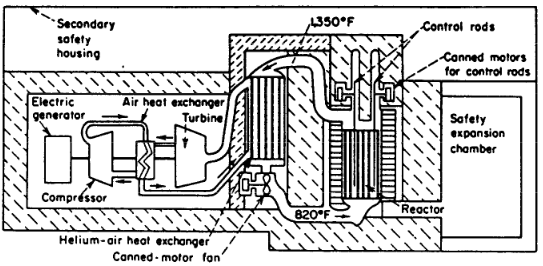
\includegraphics[width=0.6\linewidth]{figures/daniels-1}
\caption{Side-View of the 1955 Daniels' Concept, \cite{simnad_early_1991}}
\label{fig:daniels-1}
\end{figure}
\begin{figure}[h!]
\centering
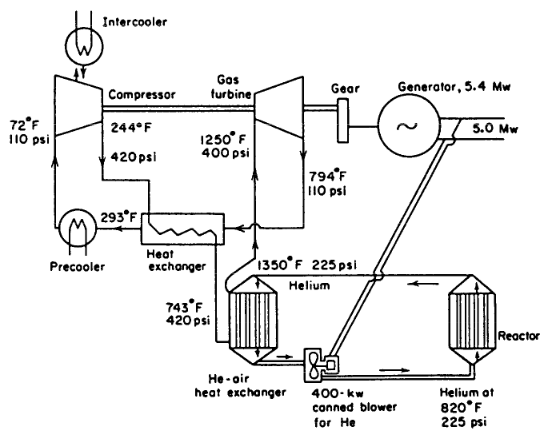
\includegraphics[width=0.6\linewidth]{figures/daniels-2}
\caption{Diagram of Coolant Flow in the 1955 Daniel's Concept, \cite{simnad_early_1991}}
\label{fig:daniels-2}
\end{figure}

Figures \ref{fig:daniels-1} and \ref{fig:daniels-2} show the 1955 concept in the design by Daniels et al.  A key difference between the Farrington Daniels et al designs and modern HTGRs is the fuel form.  While modern designs use TRISO particles embedded in graphite, the Daniels et al design used solid graphite blocks, with channels for both coolant and fuel.  Within the fuel channels, fuel loaded in either a pellet or cartridge form, both a mixture of 10$\%$ uranium dicarbide and graphite powder.  In addition to these fuel channels, the design included an outer ring of graphite reflector in which used thorium to breed $^{233}U$.  Control rods were of a boron-containing molybdenum.  Steel wires that would melt in the case of an accident held more of the same above the core, and would drop the safety rods in case of an accident \cite{simnad_early_1991}.

\subsection{Earliest Operational HTGRs}

The earliest operational HTGRs: the AVR, from Germany; Dragon, operating in the UK; and Peach Bottom 1, in the US; came online in the 1960s \cite{beck_high_nodate}.  The following sections discuss these three early reactors and the impact of knowledge and experience gained during their operation.

\subsubsection{Dragon}

The Dragon prismatic HTGR was a test reactor operated in Winfrith, UK, by the Organization for Economic Co-operation and Development from 1964 to 1975, making it the oldest of the reactors discussed in this chapter.  It operated with inlet and outlet temperatures of 350 \textdegree C and 750 \textdegree C, respectively, and at 20MWt \cite{beck_high_nodate}.  Dragon's main purpose was to test reactor materials, with an emphasis on fuels.  It originally used uranium and thorium as fuel but switched to a purely uranium-based fuel with a lower enrichment later in life.  The fuel elements themselves were similar in shape to the Daniels' design --- hexagonal prisms with fuel rod channels.

Contrary to the fuel philosophy seen today, Dragon originally allowed fission products released from fuel elements into the circulating helium coolant.  The fission products are then purged from the helium.  However, Dragon later switched to a coated-particle fuel when it became clear that having such fission product releases were difficult to manage \cite{simnad_early_1991}.

\subsubsection{Peach Bottom 1}

Peach Bottom 1 operated from 1966 to 1974, by the Philadelphia Electric Company and stationed in Delta, Pennsylvania \cite{beck_high_nodate},\cite{noauthor_peach_nodate}.  It was the first operational HTGR in the US, and the first to produce electric power.  It was slightly larger than Dragon, at a nameplate capacity of 115 MWt/40MWe and a slightly lower operating temperature range at 327\textdegree  C to 700\textdegree  C inlet to outlet \cite{beck_high_nodate}.  Like Dragon, Peach Bottom 1 was a prismatic reactor; however, Peach Bottom used coated uranium and thorium carbide particles coated by a single layer of pyrolytic carbon.  However, after multiple fuel failures, Peach Bottom upgraded to bistructural isotropic, or BISO, fuels by adding an additional layer.  Peach Bottom would later upgrade the fuel once again by adding a silicon carbide layer, forming TRISO particles \cite{beck_high_nodate}.  One operational benefit of upgrading to TRISO particles from BISO particles was that the superior fission product retention meant that Peach Bottom 1 could remove the helium purging systems.  In addition to the inner fuel region, Peach Bottom, like the Daniels et al design, bred $^{233}U$ in an outer region using thorium.

Beyond changing the number and materials for fuel coatings, the experiences in Peach Bottom 1 helped to develop HTGR fuel elements.  Operators saw that they could dilute the fuel with graphite moderating material more so than other diluents.  This has the advantage of saving fuel material, improving heat transfer, and reducing radiation damage.  Additionally, operational experience showed that, in order to prevent the creation and buildup of $^{236}U$ and $^{237}Np$, which are neutron poisons, the $^{235}U$ and $^{233}U$ should be kept separate \cite{simnad_early_1991}.  In the end, however; Peach Bottom 1 closed after the Philadelphia Electric Company determined its size made it no longer economically viable.

\subsubsection{AVR}

The Arbeitsgemeinschaft Versuchsreaktor (AVR) was an experimental pebble-bed reactor operated in and by the Jülich Research Center (in Jülich, Germany) from 1967 to 1988.  It had a capacity of 46 MWt/15MWe, with inlet and outlet temperatures of 275\textdegree  C and 950\textdegree  C \cite{beck_high_nodate}.  The AVR used a combination of uranium and thorium fuels, though it began with bi-structural isotropic (BISO) particles.  The core held around 100,000 graphite pebbles, only a third of which had fuel in them.

Despite not being built for experimental purposes, the AVR still housed many experiments that improved our body of knowledge on HTGR technology.  During the first few years of its life, the goal of the AVR was to demonstrate that it was a reliable technology --- that the reactor could operate safely, that they could control the core power and temperatures, safely shutdown, and remain sub-critical for long periods of time.  After this inital period, the AVR shifted focus to allow various experiments including: core temperature distributions, accident analysis, and fuel testing.  The AVR also shifted from highly enriched to low enriched fuel over time, which caused a variation in fuel pebble compositions, on top of the range of compositions inherent to a multi-pass pebble cycle due to varying burnup.

The AVR also provided data to validate simulations of pebble-bed reactors, and conducted an experiment to better characterize the radial distribution of temperatures in the core \cite{noauthor_results_1990}.  Operators loaded a number of marked pebbles into the core, each housing a series of wires that would melt at a certain temperature, the lowest being 655\textdegree  C, the highest 1280\textdegree  C.  Those conducting the test tracked pebble location using flow data, and examined them after they were ejected to determine what temperatures the pebbles experienced.  Despite the outlet temperature being 950\textdegree  C, multiple pebbles experienced a temperature greater than or equal to the 1280\textdegree C maximum temperature in the melt wires.  The results noted that these pebbles went through a zone with a spike in local power density, which could account for the temperature spike \cite{noauthor_results_1990}.

The AVR also demonstrated the inherent safety of HTGR reactors in accident scenarios by purposefully causing failures of the active cooling system.  In the first, the coolant blowers were shutoff, and no shutdown rods inserted, while operating at full power.  The operators additionally shut the main circuit valves to prevent natural circulation to regions outside the active core.  Overall, the changes to core temperatures were unremarkable.  The hottest regions cooled, while the coldest regions warmed up.  Additionally, due to negative temperature feedback coefficients, the reactor power immediately declined in response to the transient event.  The temperature slowly rose to 2 MW again over 24 hours, leveling out around 300 kW.  A further test provided data on loss of coolant and depressurization accidents.  As before, the core temperature changes were unremarkable.  The upper core region cooled, while the lower, originally cooler core region slowly rose in temperature.  The experiment's thermal data helped validate HTGR computer models by providing a real-world benchmark.  This meant that the results to aid in the analysis of other HTGRs \cite{noauthor_results_1990}.

Beyond accident safety, the AVR allowed for testing and demonstration of the safety qualities of TRISO and BISO fuel elements; especially relating to high temperature tolerance, and fission product retention.  Initial tests used BISO based pebbles, then later transitioned to TRISO, then to low-enriched-uranium (LEU) TRISO pebbles.  The TRISO-LEU pebbles had good fission product retention compared with their BISO-based predecessors, based on the the activity of samples taken from the circulating helium.  Beyond radioisotopes being directly released into the coolant gas, the AVR also showed that in order to accurately characterize the source term of am HTGR pebble bed reactor, one must take the dust from the pebbles into account.  Dust from the pebbles bumping and scraping against each other deposited on reactor surfaces in the primary loop.  Sixty kg of dust had accumulated by the end of the reactor's life, which averages to 3 kg of dust each year.  Measurements of specific activity in the dust showed that the activities of $^{137}Cs$, $^{134}Cs$, $^{131}I$, $^{90}Sr$, and $^{60}Co$ were on the order of $\frac{Bq}{g}$ (see Table \ref{table:gas-acc} and Table \ref{table:dust-acc}).  Even though relatively little dust accumulates, the activity of this dust is fairly high, especially compared to the activity of the coolant gas \cite{noauthor_results_1990}.  This dust can become mobile in an accident scenario, potentially being released into the environment, or inhaled.

\begin{table}[h!]
\centering
\caption{Helium Coolant Specific Activities in the AVR, reproduced from Table 2 in \cite{gottaut_results_1990} --- Results of experiments at the AVR Reactor by H.Gottaut and K.Krüger}
\begin{tabular}{ c   c }
\hline
Isotope & Specific Activity in Primary Coolant Gas $[\frac{Bq}{m^3}]$  \\
\hline
$\sum$ Fission noble gas & $4.6\times10^{08}$  \\
$^{3}H$ & $3.7\times10^{07}$  \\
$^{14}C$ & $1.9\times10^{07}$  \\
$^{137}Cs$ & $3.0\times10^{02}$ \\
$^{131}I$ & $5.2\times10^{02}$ \\
$^{110m}Ag$ & $4.9\times10^{01}$  \\
$^{90}Sr$ & $2.0\times10^{02}$  \\
$^{60}Co$ & $1.0\times10^{01}$ \\
\hline
\end{tabular}
\label{table:gas-acc}
\end{table}
\begin{table}[h!]
\centering
\caption{Pebble Dust Specific Activities, reproduced from Table 3 in \cite{noauthor_results_1990} --- Results of experiments at the AVR Reactor by H.Gottaut and K.Krüger}
\begin{tabular}{ c   c }
\hline
Isotope & Specific Activity in Dust $[\frac{Bq}{g}]$  \\
\hline
$^{137}Cs$ & 2 - 96  \\
$^{134}Cs$ & 0.7 - 27 \\
$^{131}I$ & 0 - 3  \\
$^{110m}Ag$ & 0.1 - 43 \\
$^{89}Sr$ & 0.6 - 42 \\
$^{90}Sr$ & 19 - 363  \\
$^{60}Co$ & 0.2 - 8 \\
\hline
\end{tabular}
\label{table:dust-acc}
\end{table}

\chapter{Literature Review}
Literature review

**give first instance of triso/htgr/pebble bed, etc, then fast forward to today**

first concept:

PBMR
\begin{itemize}
\item South-African pebble bed HTGR based on German HTGR reactor technology
\item Designs had thermal power capacities 200+
\item currently in "care and maintenance"
\item various 
\end{itemize}  


NGNP

Cisneros

Xenergy (Xe-100,etc)

**mention these briefly**

\url{https://www.sciencedirect.com/science/article/pii/S0306454918303748?casa_token=t58RGuIX6VAAAAAA:2dcGCyANultpSMw7DSSIGGvmzdgpH3wr6fWw50j2awnpkBVItZ5zxoyOxQVGpGcIFNMRlPs}

\url{https://www.mdpi.com/1996-1073/8/12/13938}

\url{https://onlinelibrary.wiley.com/doi/full/10.1002/er.4542?casa_token=Q78UeM8i1XkAAAAA%3ArcPa5kUAo6c04Ykmgu5KY5rTcEBcC2cQa5lT7ynMqE7UvTR5bqZ28Xxh5zq3-7WtlydJu1_PeVpr}



\chapter{Methodology}
\label{sec:methods}
\begin{table}[h!]
\centering
\caption{Geometric and Internal Core Parameters in the Sangamon Reactors}
\begin{tabular}{ c  c  c }
\hline
Parameter & Sangamon200 \cite{harlan_x-energy_2018}, \cite{harlan_ans_2017} & Sangamon20 \\
\hline
Thermal Power [MW] & 200 & 20 \\
Average Core Temperature [K] & 800 & 800 \\
Enrichment [wt\%] & 15.5\% & 19.75\% \\
Average Core Pressure [MPa] & 5.9 & 5.9 \\
Outer Core Radius [cm] & 216 & 165 \\
Outer Core Height [cm] & 1150 & 330 \\
Reflector Thickness [cm] & 92 & 75 \\
Number of Pebbles & 220,000 & 22,680 \\
Packing Fraction [\%] & 53.0 & 56.0 \\
\hline
\end{tabular}

\label{table:params1}
\end{table}

All neutronics simulations are performed using Serpent2.0 \cite{leppanenjaakko_serpent_2015} .  Pebbles are individually modeled, with locations generated using Serpent2.0's particle dispersal routine (***should I go into more detail on the dispersal routine?***).  Each pebble in the full-core model has the TRISO-filled "fueled-core" homogenized by volume.
\\
\begin{figure}[H]
\centering

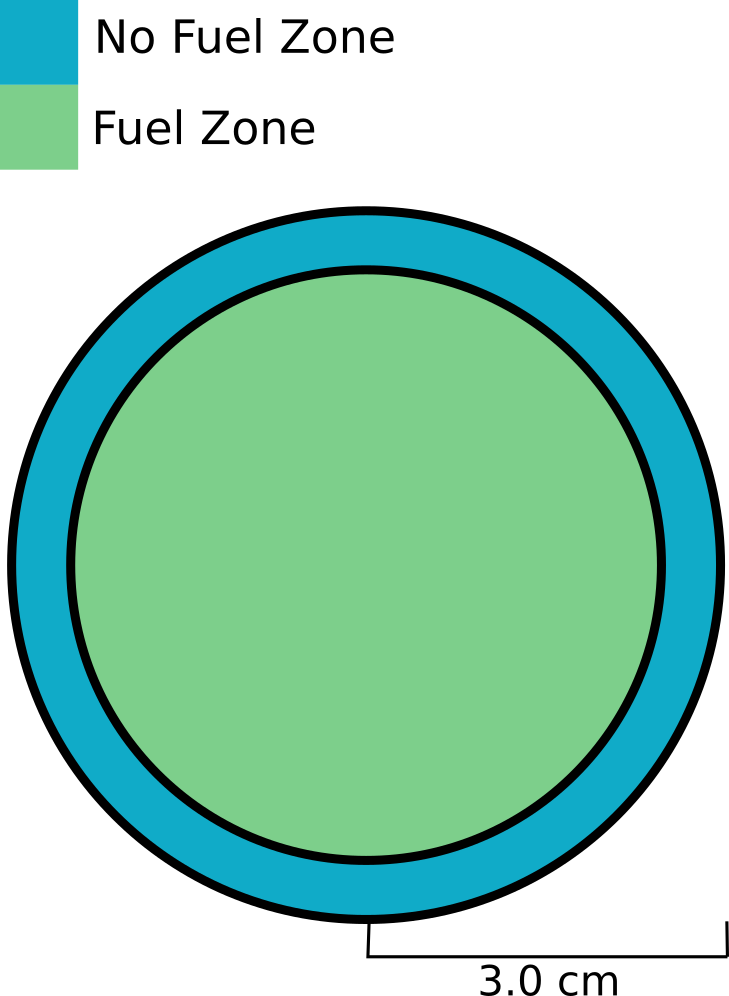
\includegraphics[width=0.5\linewidth]{figures/pebble-zones.png}
\caption{Pebble Zones}
\label{fig:pebb-zone1}
\end{figure}


\begin{table}[h!]
\centering

\caption{Pebble Parameters}
\begin{tabular}{ c  c }
\hline
Parameter & Value \\
\hline
Fueled-Center Radius [cm] & 2.5 \\
Graphite Outer Shell Thickness [cm] & 0.5 \\
Total Radius [cm] & 3.0 \\
TRISO Particles per Pebble & 18,000 \\
\hline
\end{tabular}
\label{table:peb-params}
\end{table}


\begin{figure}[H]
\centering

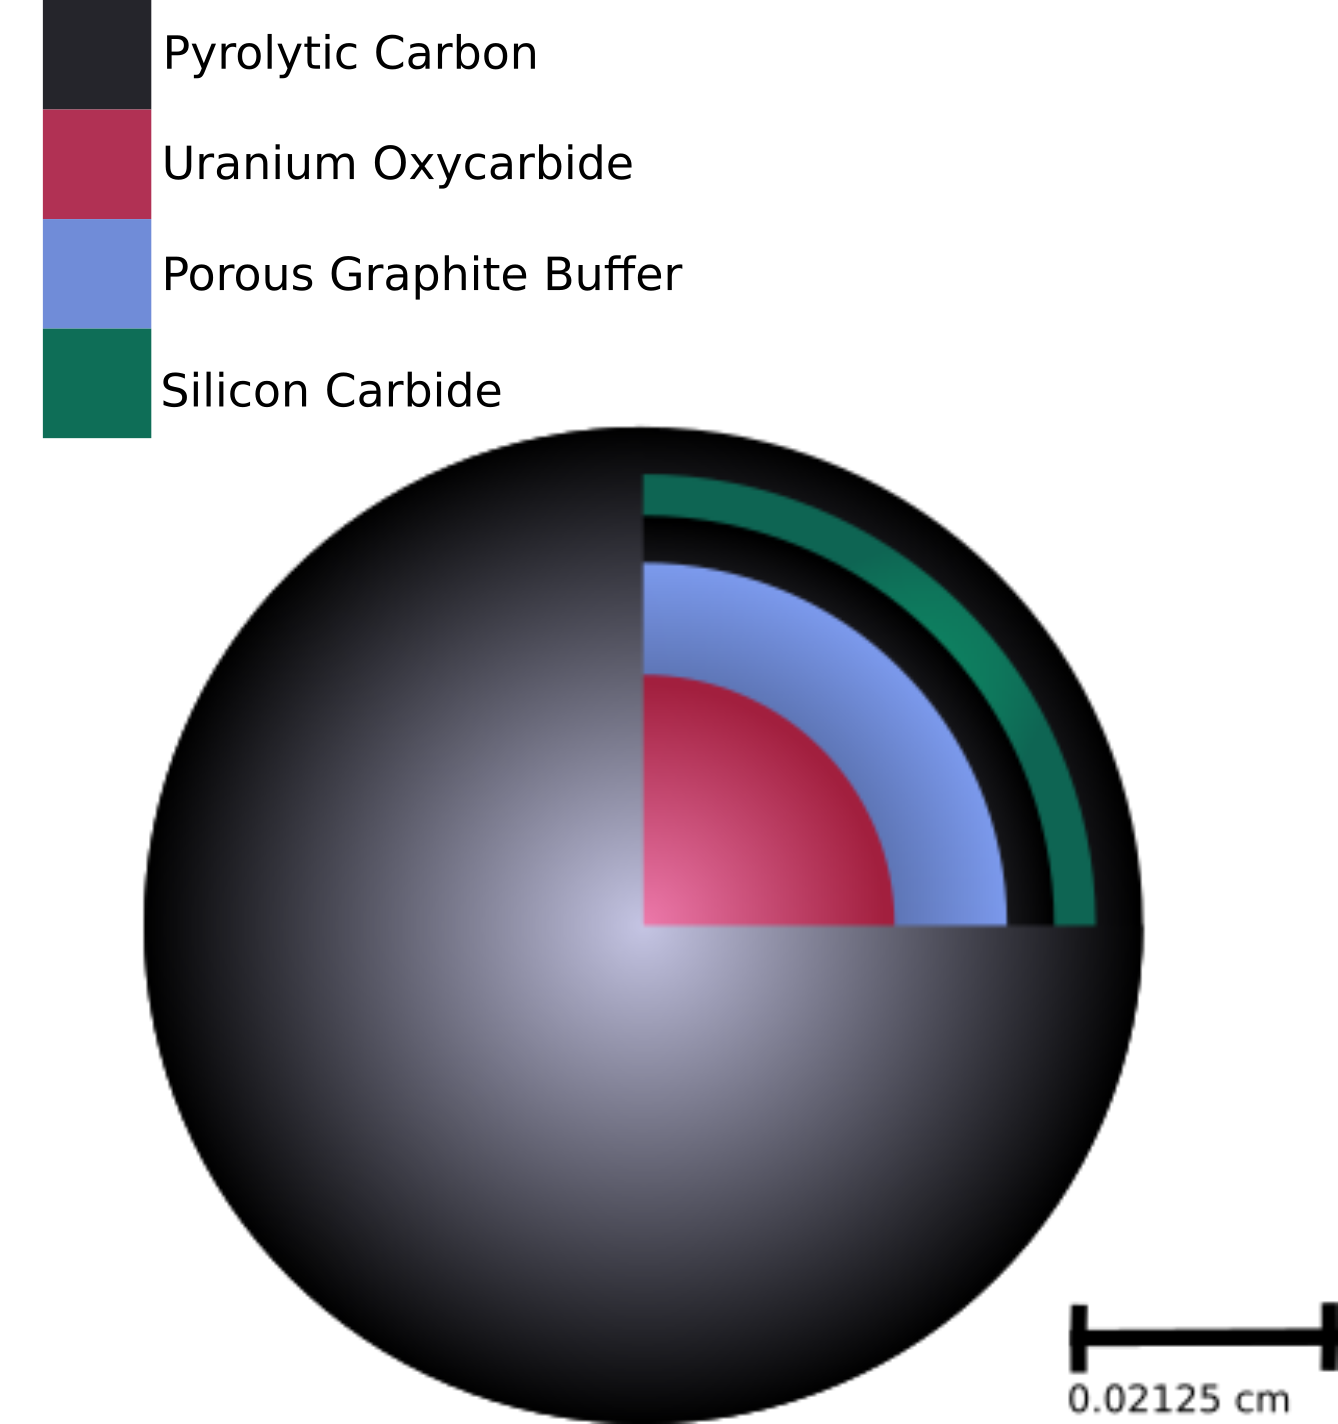
\includegraphics[width=0.5\linewidth]{figures/trisos-r-like-onions.png}
\caption{TRISO Particle Layers}
\label{fig:particle-layer}
\end{figure}

\begin{table}[h!]
\centering

\caption{Particle Parameters Used in Monte Carlo Simulations}
\begin{tabular}{ c  c }
\hline
Parameter & Value [cm] \\
\hline 
Uranium Oxycarbide Kernel Radius & 0.02125 \\
Graphite Layer Thickness & 0.03075 \\
Inner Pyrolytic Carbon Layer Thickness & 0.03475 \\
Silicon Carbide Layer Thickness & 0.03825 \\
Outer Pyrolytic Carbon Layer Thickness & 0.04225 \\
\hline
\end{tabular}
\label{table:particle-params}

\end{table}

\begin{table}[h!]
\centering
\begin{tabular}{ c  c }
\hline
Parameter & Value \\
\hline
Fueled-Center Radius [cm] & 2.5 \\
Graphite Outer Shell Thickness [cm] & 0.5cm \\
Total Radius [cm] & 3.0 \\
TRISO Particles per Pebble & 18,000 \\
\hline
\end{tabular}
\caption{Pebble Parameters}
\label{table:params2}
\end{table}
\begin{table}[h!]
\centering
\begin{tabular}{|| c || c |}
\hline
Parameter & Value \\
\hline \hline
Uranium Oxycarbide Kernel Radius [cm] & 0.02125 \\
Graphite Layer Thickness [cm] & 0.03075 \\
Inner Pyrolytic Carbon Layer Thickness [cm] & 0.03475 \\
Silicon Carbide Layer Thickness [cm] & 0.03825 \\
Outer Pyrolytic Carbon Layer Thickness [cm] & 0.04225 \\
\hline
\end{tabular}
\caption{Particle Parameters}
\label{table:params3}
\end{table}
\\
Fuel isotopic composition aside, the pebbles are identical in both reactor designs.  Both reactors feature a 6-month multi-pass cycle, with each pass through the core taking 6 months.  That is to say, a pebble will go through six 6-month passes before leaving the core.

\section{Sangamon200}
Sangamon200 is a 200 MWth helium cooled reactor.  It is an Xe-100 inspired design, and further informed by previous work on reactors such as the PBMR.  Parameters are generally pulled from literature, or made by averaging given values in literature.  For unspecified reactor dimensions, a rough estimate is approximated by assuming provided figures of a design are to scale, and converting measurements in pixels to cm.

Sangamon200 is still, however, a simplification of previously established designs.  The "cone" formed at the top and bottom of the reactor core is averaged to a flat surface, to create a cylindrical core shape.  The graphite reflector surrounds it, with no barriers between the reflector and helium/pebble-filled active core region.  In effect, the reflector is the container for the pebbles.  These are the only simulated parts of the reactor.  It is assumed no control rods are being used.  In addition, the graphite reflector is defined as a solid cylindrical shell.

While Sangamon200 is not the focus of this assessment, some neutronics features were determined to aid in Sangamon20's design.  A surface current detector was placed in the reflector, just inside the outer bound of the reflector, as shown in \ref{fig:det-place}.

\begin{figure}[H]
\centering
\resizebox{0.5\textwidth}{!}{%
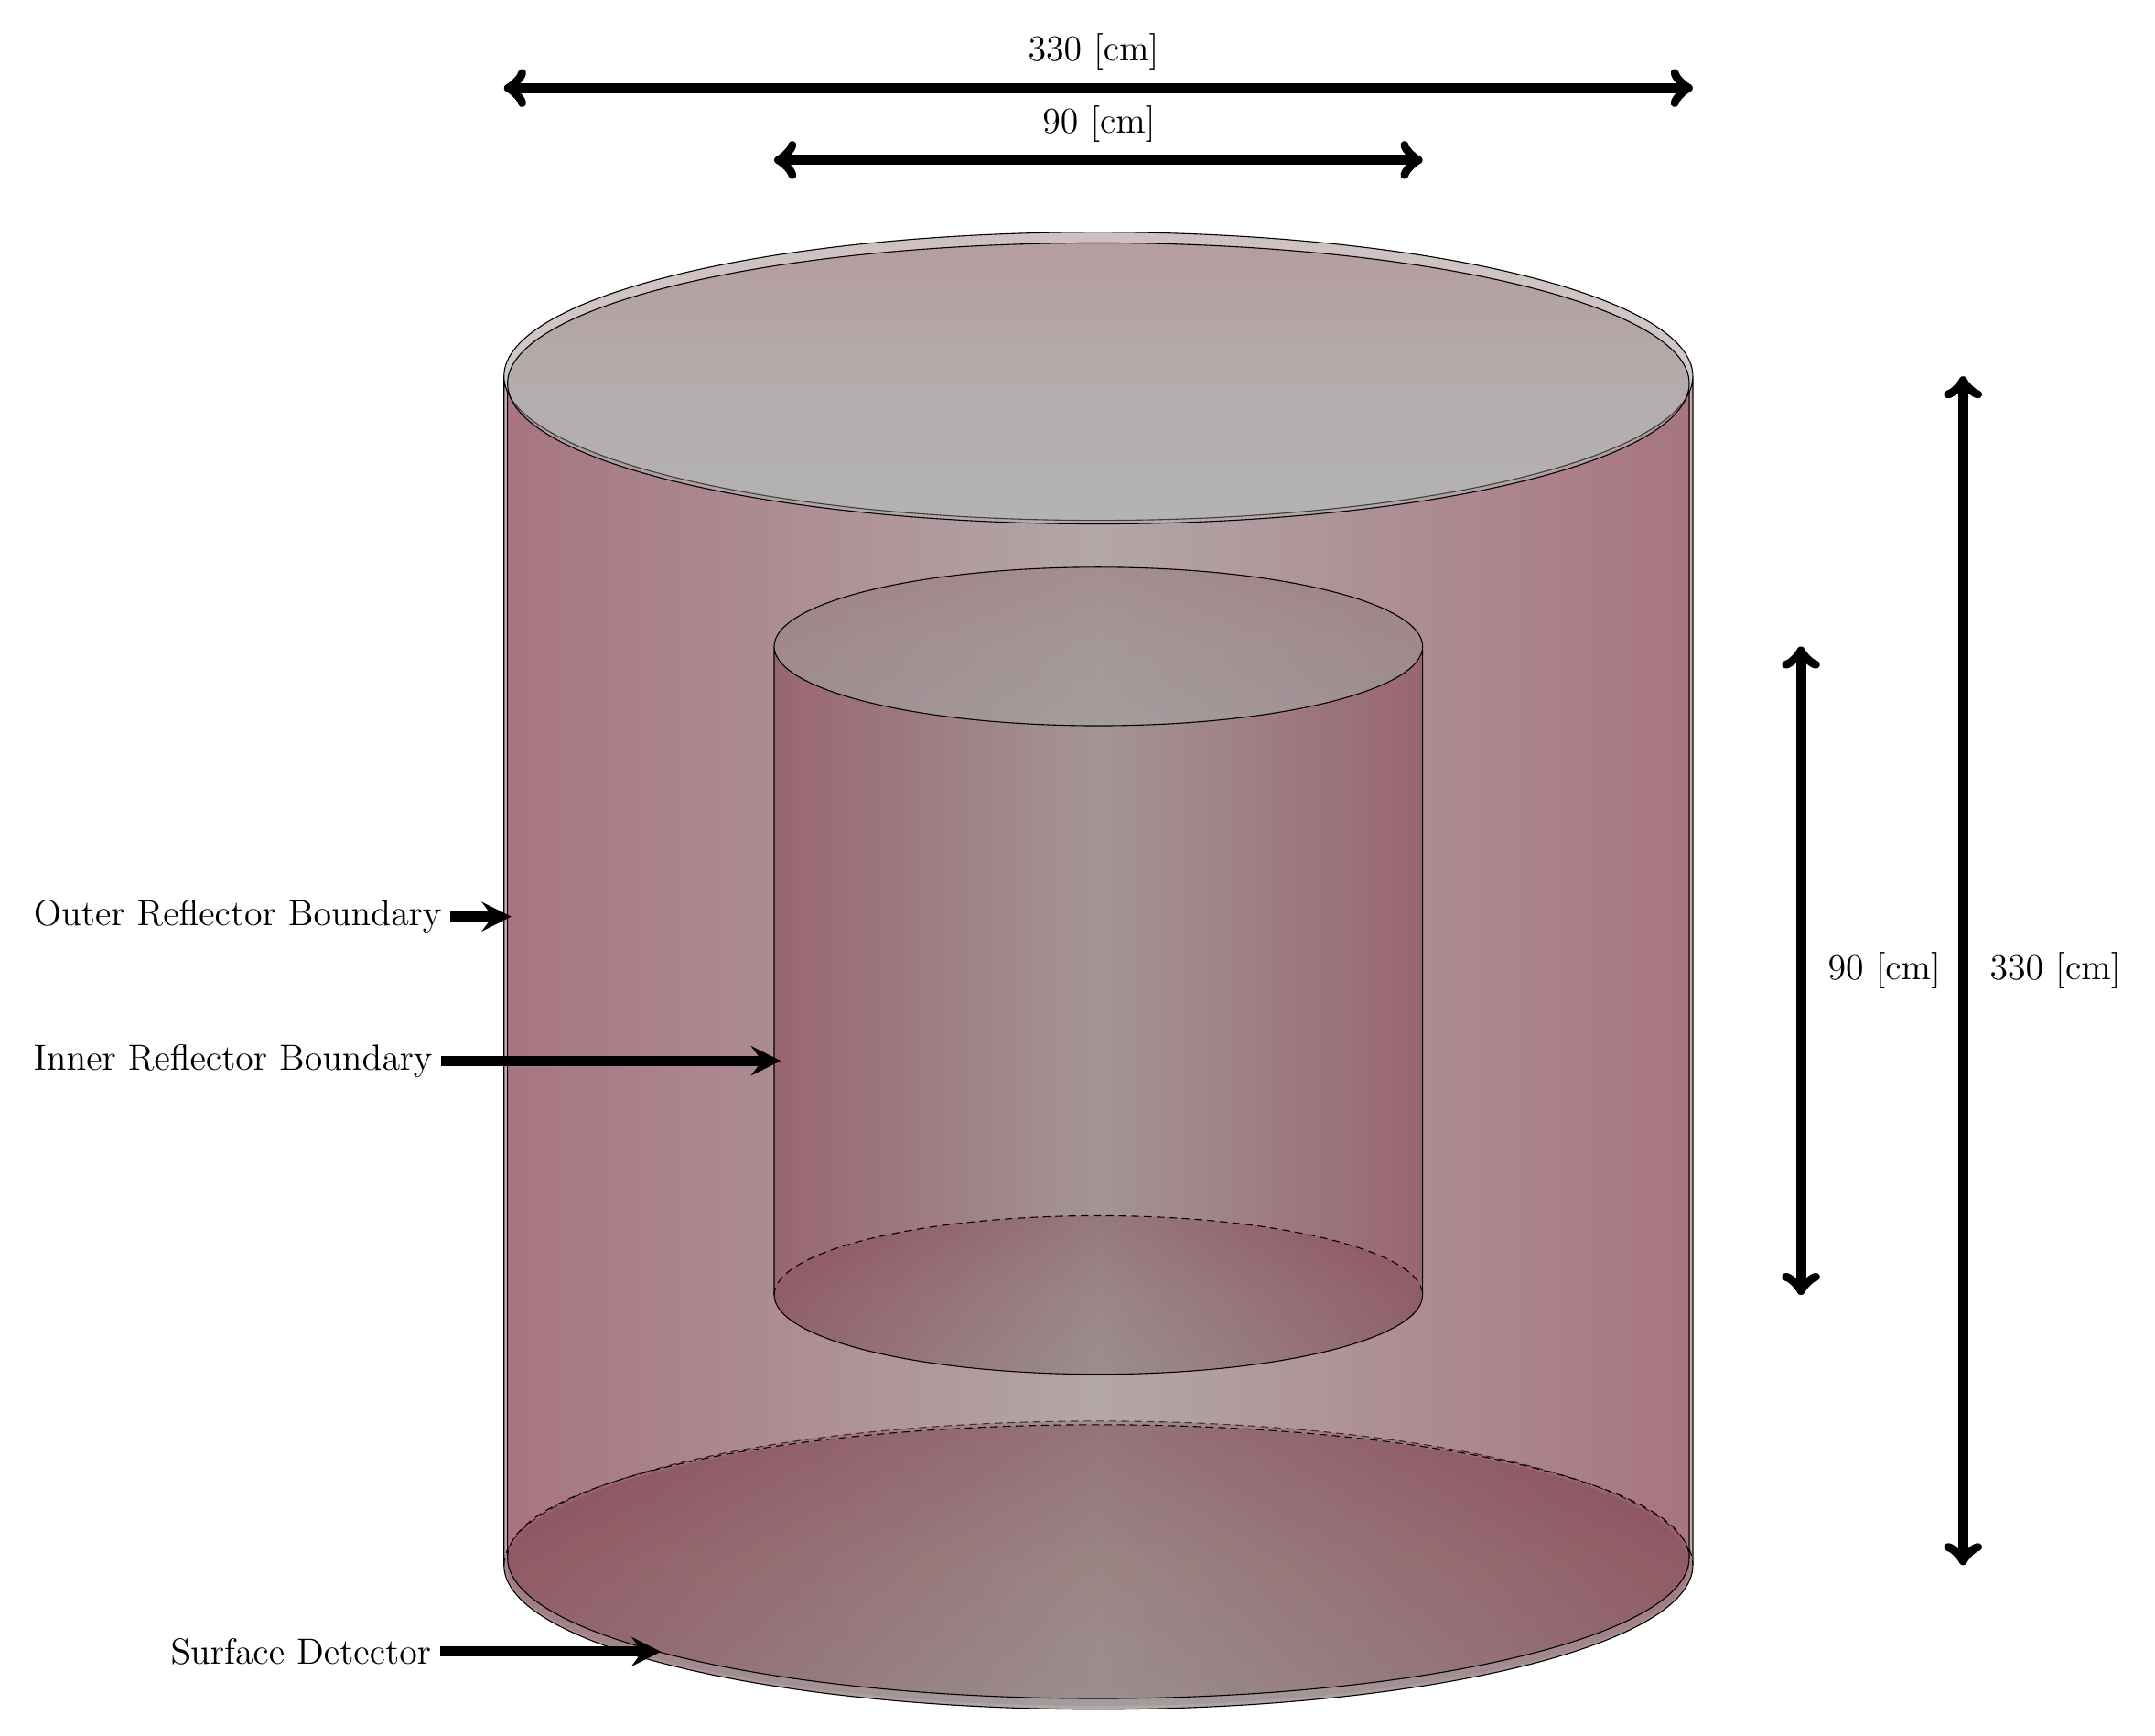
\begin{tikzpicture}
\fill[top color=pink!50!purple,bottom color=pink!10,middle color=pink,shading=axis,opacity=0.25] (0,0) circle (8.25cm and 2.0cm);
\fill[left color=pink!50!purple,right color=pink!50!purple,middle color=pink!50,shading=axis,opacity=0.25] (8.25,0) -- (8.25,16.5) arc (360:180:8.25cm and 2.0cm) -- (-8.25,0) arc (180:360:8.25cm and 2.0cm);
\fill[top color=pink!90!,bottom color=pink!2,middle color=pink!30,shading=axis,opacity=0.25] (0,16.5) circle (8.25cm and 2.0cm);
\draw (-8.25,16.5) -- (-8.25,0) arc (180:360:8.25cm and 2.0cm) -- (8.25,16.5) ++ (-8.25,0) circle (8.25cm and 2.0cm);
\draw[densely dashed] (-8.25,0) arc (180:0:8.25cm and 2.0cm);

\fill[top color=pink!50!purple,bottom color=pink!10,middle color=pink,shading=axis,opacity=0.25] (0,0.0) circle (8.2cm and 1.95cm);
\fill[left color=pink!50!purple,right color=pink!50!purple,middle color=pink!50,shading=axis,opacity=0.25] (8.2,0.1) -- (8.2,16.4) arc (360:180:8.2cm and 1.95cm) -- (-8.2,0.1) arc (180:360:8.2cm and 1.95cm);
\fill[top color=pink!90!,bottom color=pink!2,middle color=pink!30,shading=axis,opacity=0.25] (0,16.4) circle (8.2cm and 1.95cm);
\draw (-8.2,16.3) -- (-8.2,0.1) arc (180:360:8.2cm and 1.95cm) -- (8.2,16.3) ++ (-8.2,0.1) circle (8.2cm and 1.95cm);
\draw[densely dashed] (-8.2,0.1) arc (180:0:8.2cm and 1.85cm);

\fill[top color=pink!50!purple,bottom color=pink!10,middle color=pink,shading=axis,opacity=0.25] (0,3.75) circle (4.5cm and 1.1cm);
\fill[left color=pink!50!purple,right color=pink!50!purple,middle color=pink!50,shading=axis,opacity=0.25] (4.5,3.75) -- (4.5,12.75) arc (360:180:4.5cm and 1.1cm) -- (-4.5,3.75) arc (180:360:4.5cm and 1.1cm);
\fill[top color=pink!90!,bottom color=pink!2,middle color=pink!30,shading=axis,opacity=0.25] (0,12.75) circle (4.5cm and 1.1cm);
\draw (-4.5,12.75) -- (-4.5,3.75) arc (180:360:4.5cm and 1.1cm) -- (4.5,12.75) ++ (-4.5,3.75) (0,12.75) circle (4.5cm and 1.1cm);
\draw[densely dashed] (-4.5,3.75) arc (180:0:4.5cm and 1.1cm);

\node [anchor=west] (out-ref) at (-14.9, 9) {\Large Outer Reflector Boundary};
\node [anchor=west] (in-ref) at (-14.9, 7) {\Large Inner Reflector Boundary};
\node [anchor=west] (det) at (-13, -1.2) {\Large Surface Detector};

\draw [-stealth, line width=4pt, black] (out-ref) -- ++(3.8,0);
\draw [-stealth, line width=4pt, black] (in-ref) -- ++(7.6,0);
\draw [-stealth, line width=4pt, black] (det) -- ++(5.0,0);

\draw [-stealth, <->, line width=4pt, black] ++(-8.25,20.5) -- ++(16.5,0);
\draw [-stealth, <->, line width=4pt, black] ++(12,0) -- ++(0,16.5);

\node [anchor=west] (out-h) at (12.25, 8.25) {\Large 330 [cm]};
\node [anchor=west] (out-d) at (-1.1, 21.0) {\Large 330 [cm]};

\draw [-stealth, <->, line width=4pt, black] ++(-4.5,19.5) -- ++(9,0);
\draw [-stealth, <->, line width=4pt, black] ++(9.75,3.75) -- ++(0,9.0);

\node [anchor=west] (in-h) at (10.0, 8.25) {\Large 90 [cm]};
\node [anchor=west] (in-d) at (-0.9, 20.0) {\Large 90 [cm]};

\end{tikzpicture}
 }%
\caption{Detector Placement Inside Reflector in Sangamon200 and Sangamon20}
\label{fig:det-place}

\end{figure}


This detector measures the outward neutron current (*** serpent outputs units of [number/s], is current still the best word? ***) in $[\frac{\#}{s}]$.  To arrive at the unit of $[\frac{\#}{cm^2s}]$ most are familiar with, the reported outward current is divided by the detector's surface area thus:
\begin{equation}
J^+ [\frac{\#}{cm^2s}] = \frac{J^+ [\frac{\#}{s}]}{S_{det}[cm^2]}
\end{equation}

After accounting for the surface area, the outward current at the detector is 7.351e+11.

\section{Sangamon20}

Sangamon20 is a 20 MWth helium-cooled pebble bed reactor, fueled with 19.75\% enriched uranium oxycarbide.  While the capacity of Sangamon20 is 10\% that of Sangamon200, it isn't accurate to simply scale Sangamon200's dimensions down to 10\% of their original values.

\subsection{Inner Core Volume Determination}

The first assumption made in the scale-down is that Sangamon200 and Sangamon20 have the same power density, or $\frac{\text{kW}}{\text{g fuel}}$ (*** I called this "power density" as that is how serpent refers to this value.  But, given that it is per unit mass, is "specific power" a better term?***).

It is simple enough to calculate the mass of fuel in Sangamon200:


\begin{align}
M_{f,200} &= \frac{4}{3}\pi r_{u}^3 \rho_{u} n_{T} n_{p,200}
\intertext{where}
M_{f,200}&= \mbox{ mass of fuel in Sangamon200[g]}\nonumber\\
r_{u}&= \mbox{the radius of the UCO kernel inside a TRISO particle[cm]}\nonumber\\
\rho_{u}&= \mbox{ the density of UCO in [$\frac{g}{cc}]$}\nonumber\\
n_{T}&= \mbox{ number of TRISO particles in one pebble}\nonumber\\
n_{p}&= \mbox{ number of pebbles in Sangamon200}
\end{align}


Using the parameters in \ref{table:params1}, the power density of Sangamon200 and Sangamon20 is 0.11 $[\frac{kW}{g}]$.  With a power capacity of 20 MWth, one can calculate the total mass of UCO in Sangamon20 as
\begin{equation}
M_{f,20} = \frac{20*10^3 [kW]}{0.11[\frac{kW}{g}]} = 181818.18 [g]
\end{equation}
The mass of fuel in a single pebble can be found using the density of UCO and the total volume of UCO kernels in a single pebble, as above.  The number of pebbles in the entire reactor, then, is found by dividing the total mass of fuel by the mass of fuel in one pebble, as follows:

\begin{equation}
n_{p,20} = \frac{M_{f,20}}{\frac{4}{3}r_{u}^3n_{T}\rho_{u}}
\end{equation}

Rounding up - there can only be complete pebbles - we arrive at the number of pebbles in \ref{table:params1}.

Knowing the number of pebbles is insufficient - the exact dimensions of the active core region are still undefined.  To determine the volume of this space, the concept of the packing fraction - the ratio of the volume of objects (the pebbles) to the total volume of their container (the active core) - can be used.  The packing of even uniform objects in a 3-dimensional space is a complicated problem, often analyzed in the context of material studies or grain silos \cite{tulluri_analysis_nodate}.  For this reactor, it is assumed the pebble behavior can be described as random loose packing \cite{tulluri_analysis_nodate} - the pebbles have unsystematically fallen into the core and the core is not shaken.  Such packing generally has a packing fraction in the range of 0.56 to 0.60 \cite{tulluri_analysis_nodate}.  Using the definition of the packing fraction, and previously defined terms, the active core volume is

\begin{equation}
V_{c,20} = \frac{ n_{p,20}\frac{4}{3}\pi r_{p}^3 }{ \phi }
\end{equation}

Using the formula for the volume of a cylinder, one can plot possible sets of $r_{c,20}$ and $h_{c,20}$ that satisfy the volume requirement.

\begin{figure}[h!]
\centering
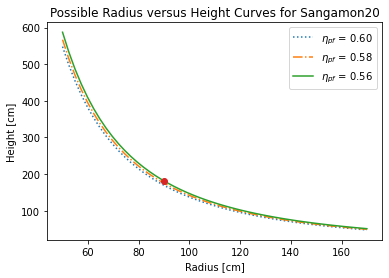
\includegraphics[width = 10cm]{figures/act-core-RH.png}
\caption{Curve of Possible Height and Radii by Packing Fraction}
\label{fig:rh-vol}
\end{figure}

The most critical configurations for a cylinder are either a \emph{square} shape, in which the height is equal to the diameter, or a \emph{flat} shape in which diameter is significantly greater than height.  As a flat shape is disadvantageous for a reactor, the former is chosen.  The point indicated in \ref{fig:rh-vol} shows the radius and height selected for Sangamon20 - a radius of 90 cm, and a height of 180 cm.

\subsection{Graphite Reflector Thickness Determination}

The reflector must be sufficiently thick to keep the reactor critical, and protect the pressure vessel.  To ensure this, the outward current must be less than or equal to the outward current in Sangamon200 at the outer reflector boundary.  The detector layout in Sangamon20 is identical to \ref{fig:det-place}.

\section{Fuel Composition}

The number of passes the pebble has theoretically experienced determines its isotopic composition.  Seven possible pebble compositions exist, one for each of the six 6-month passes, plus an additional composition for fresh pebbles.  The seven pebble compositions are represented equally in number in the core, and they are randomly distributed throughout the core.

The exact isotopic composition is approximated by running a burnup calculation using Serpent2 for a single pebble in a cube.  It uses a reflective boundary condition to simulate the presence of other pebbles or the reflector.  The void in the square is filled with helium.  While the full-core models homogenize the pebbles, the single-pebble burnup model individually models each TRISO particle.  Just as with the location of the pebbles in the full core, the Serpent2 particle dispersal routine generated the TRISO particle locations.

\begin{figure}[H]
\centering
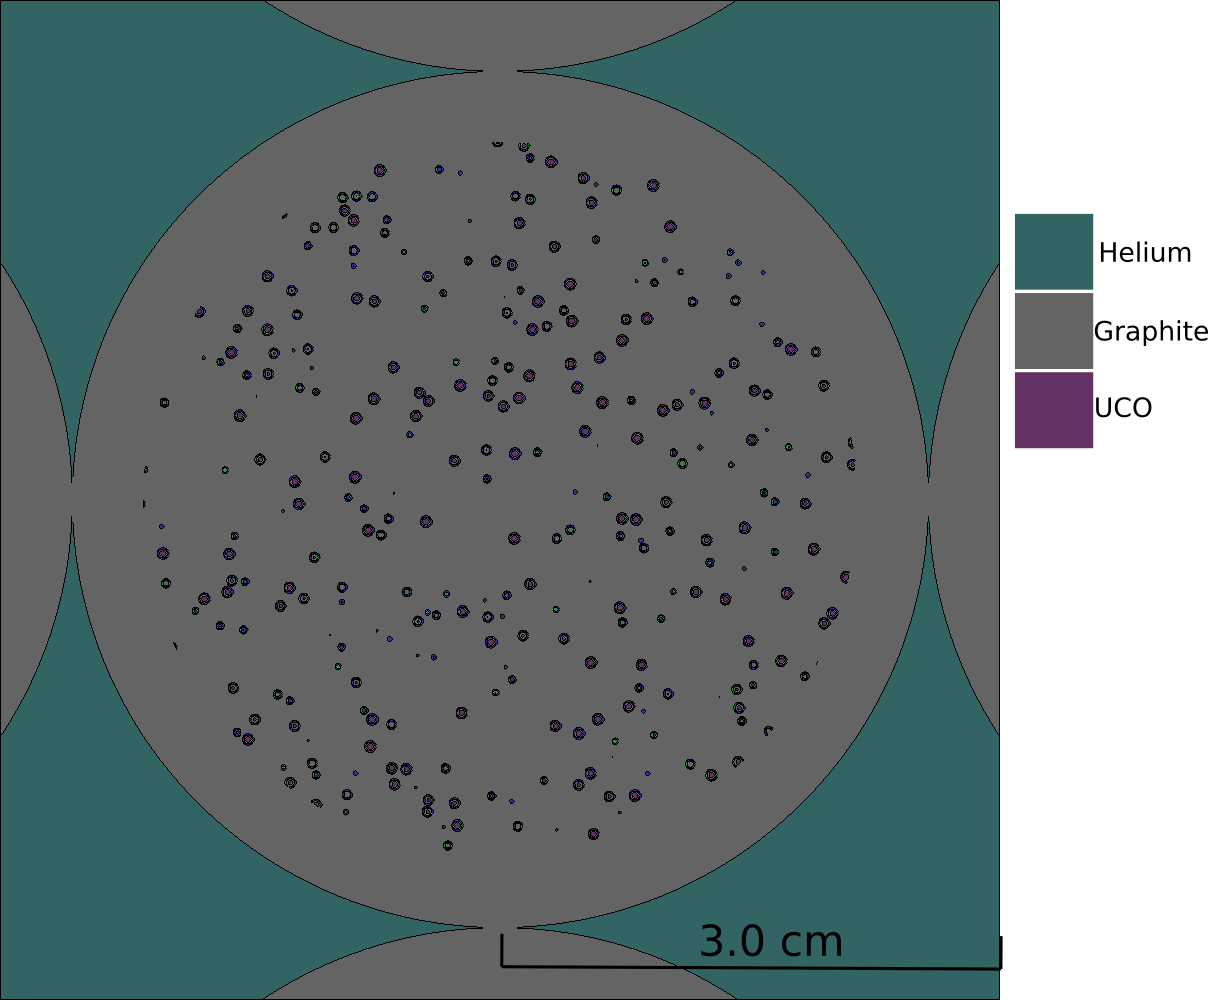
\includegraphics[width = 10cm]{figures/burn-20.png}
\caption{Geometry of the Single-Pebble Burnup Calculation for Sangamon20}
\label{fig:burn-20}
\end{figure}

Once the isotopic compositions are determined, the pebbles are homogenized by volume, to improve performance.  The volume of a TRISO particle, and more specifically, a UCO kernel, is assumed constant.

\section{Reactor Sensitivity to Pebble Locations and Symmetry}

As the pebble locations and compositions are determined randomly, it is entirely possible to have bands in the reactor where multiple pebbles of same (or similar) burnup form lines or pockets.  In the interest of better characterizing the neutronics of the reactor, a sensitivity analysis tested various pebble composition locations.  The \emph{shuffling} test maintained the pebble locations, but changed what composition the individual pebbles were.  A second test completely changed the location of the pebbles in the core by randomly dispersing them again.  The third analyzed the effects of utilizing a symmetry simplification, in order to improve computational speed.  The core was approximated using a $\frac{1}{6}$ slice.  The slice used to simplify changed in each test, shown in \ref{fig:slicetest}.  In each test, all other parameters remain the same.

\begin{figure}[h!]
\centering
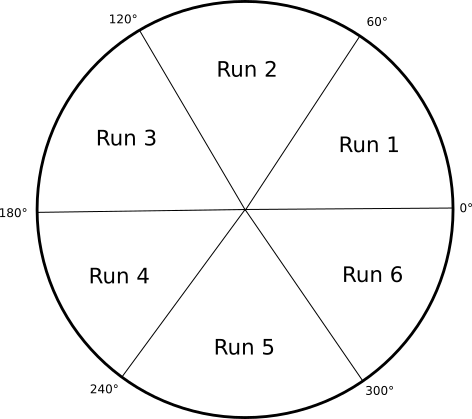
\includegraphics[width=0.6\linewidth]{figures/run-layout.png}
\caption{Symmetry Test Run Layouts}
\label{fig:slicetest}
\end{figure}

\chapter{Results}
This chapter first presents the atomic fractions of select isotopes of interest, and the fission rate/thermal flux mesh corresponding to each depletion time step.  Then, \autoref{res-control} covers the results of the basic control model. The final sections --- dedicated to homogenization (see \autoref{res-hom}), symmetry (see \autoref{res-sym}), and shuffling (see \autoref{res-shuff}) --- compare the results of these tests to the control model.

\section{Fuel Isotopic Compositions}

Serpent allows the user to set a series of burnup steps in a single simulation if desired.  For this work, the burnup steps were defined by the total days that had passed --- 6 months, 12 months, 18 months, 24 months, 30 months, and 36 months.  Other than this, all conditions are equal at each time step.

\begin{figure}[H]
\centering
%
\begin{subfigure}{0.4\textwidth}
  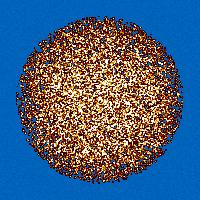
\includegraphics[width=0.95\linewidth]{figures/burn-20-bstep0}
  \caption{Fresh}
  \label{fig:bstep0}
\end{subfigure}%
%
\begin{subfigure}{0.4\textwidth}
  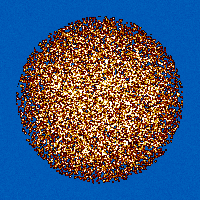
\includegraphics[width=0.95\linewidth]{figures/burn-20-bstep1}
  \caption{One Pass}
  \label{fig:bstep1}
\end{subfigure}%

\caption{Mesh Figures For Single Pebble Burnup}
\end{figure}

\begin{figure}[H]\ContinuedFloat
\centering

\begin{subfigure}{0.4\textwidth}
  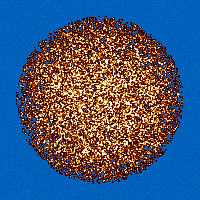
\includegraphics[width=0.95\linewidth]{figures/burn-20-bstep2}
  \caption{Two Passes}
  \label{fig:bstep2}
\end{subfigure}%
%
\begin{subfigure}{0.4\textwidth}
  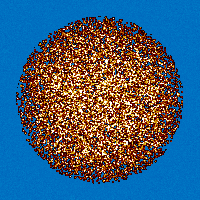
\includegraphics[width=0.95\linewidth]{figures/burn-20-bstep3}
  \caption{Three Passes}
  \label{fig:bstep3}
\end{subfigure}%

\begin{subfigure}{0.4\textwidth}
  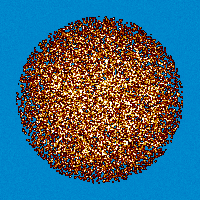
\includegraphics[width=0.95\linewidth]{figures/burn-20-bstep4}
  \caption{Four Passes}
  \label{fig:bstep4}
\end{subfigure}%
%
\begin{subfigure}{0.4\textwidth}
  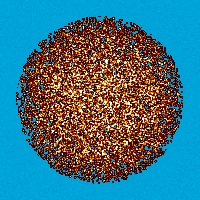
\includegraphics[width=0.95\linewidth]{figures/burn-20-bstep5}
  \caption{Five Passes}
  \label{fig:bstep5}
\end{subfigure}%

\begin{subfigure}{0.4\textwidth}
  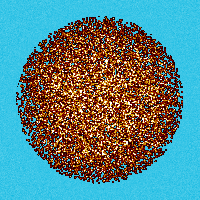
\includegraphics[width=0.95\linewidth]{figures/burn-20-bstep6}
  \caption{Six Passes}
  \label{fig:bstep6}
\end{subfigure}%
%
\caption{Mesh Figures For Single Pebble Burnup(cont.)}
\label{fig:burn-meshes}
\end{figure}

Figure \ref{fig:burn-meshes} depicts the evolution of the fission rate (hot color map) and thermal flux (cold color map) over the seven stages.  The maximum cutoff for thermal flux is 0.625 eV in these figures.  Over successive depletion steps, the fission rate decreases, and thermal flux increases.  Is is not unexpected --- as the pebble burns, the atomic fraction of fissile $^235U$ decreases, which results in a lower fission rate at each time step.  At the same time, the reduction of fissile isotopes and build up of fission products means the neutrons can have a longer lifetime before undergoing capture, resulting in a more thermalized spectrum.

But understanding the effects on simple core neutronics such as the fission rate or thermal flux is not the only reason to find the isotopic composition of the fuel.  Fission product buildup in the fuel not only has long term ramifications for spent fuel handling, but matters for our understanding of accident consequence analysis.  The potential isotopes --- and in what amounts --- that a living being or environment might be exposed to after an accident is called a source term.  As shown in Tables \ref{table:gas-acc} and \ref{table:dust-acc}, fission products can either leach into the coolant gas, or be found in the fine dust formed when the pebbles bump against each other during operation.  In an accident, this dust could be jettisoned from the \acrshort{rpv} in the case of a breach, where it could be inhaled or reach the ground or groundwater.  In order to fully understand accident consequences, one must understand the source term.  Figure \ref{fig:comps} provides the atomic fractions of isotopes of iodine, xenon, cesium, radium, thorium, uranium, and plutonium within depleted \acrshort{uco}.

\begin{figure}[H]
\centering
%
\begin{subfigure}{0.8\textwidth}
  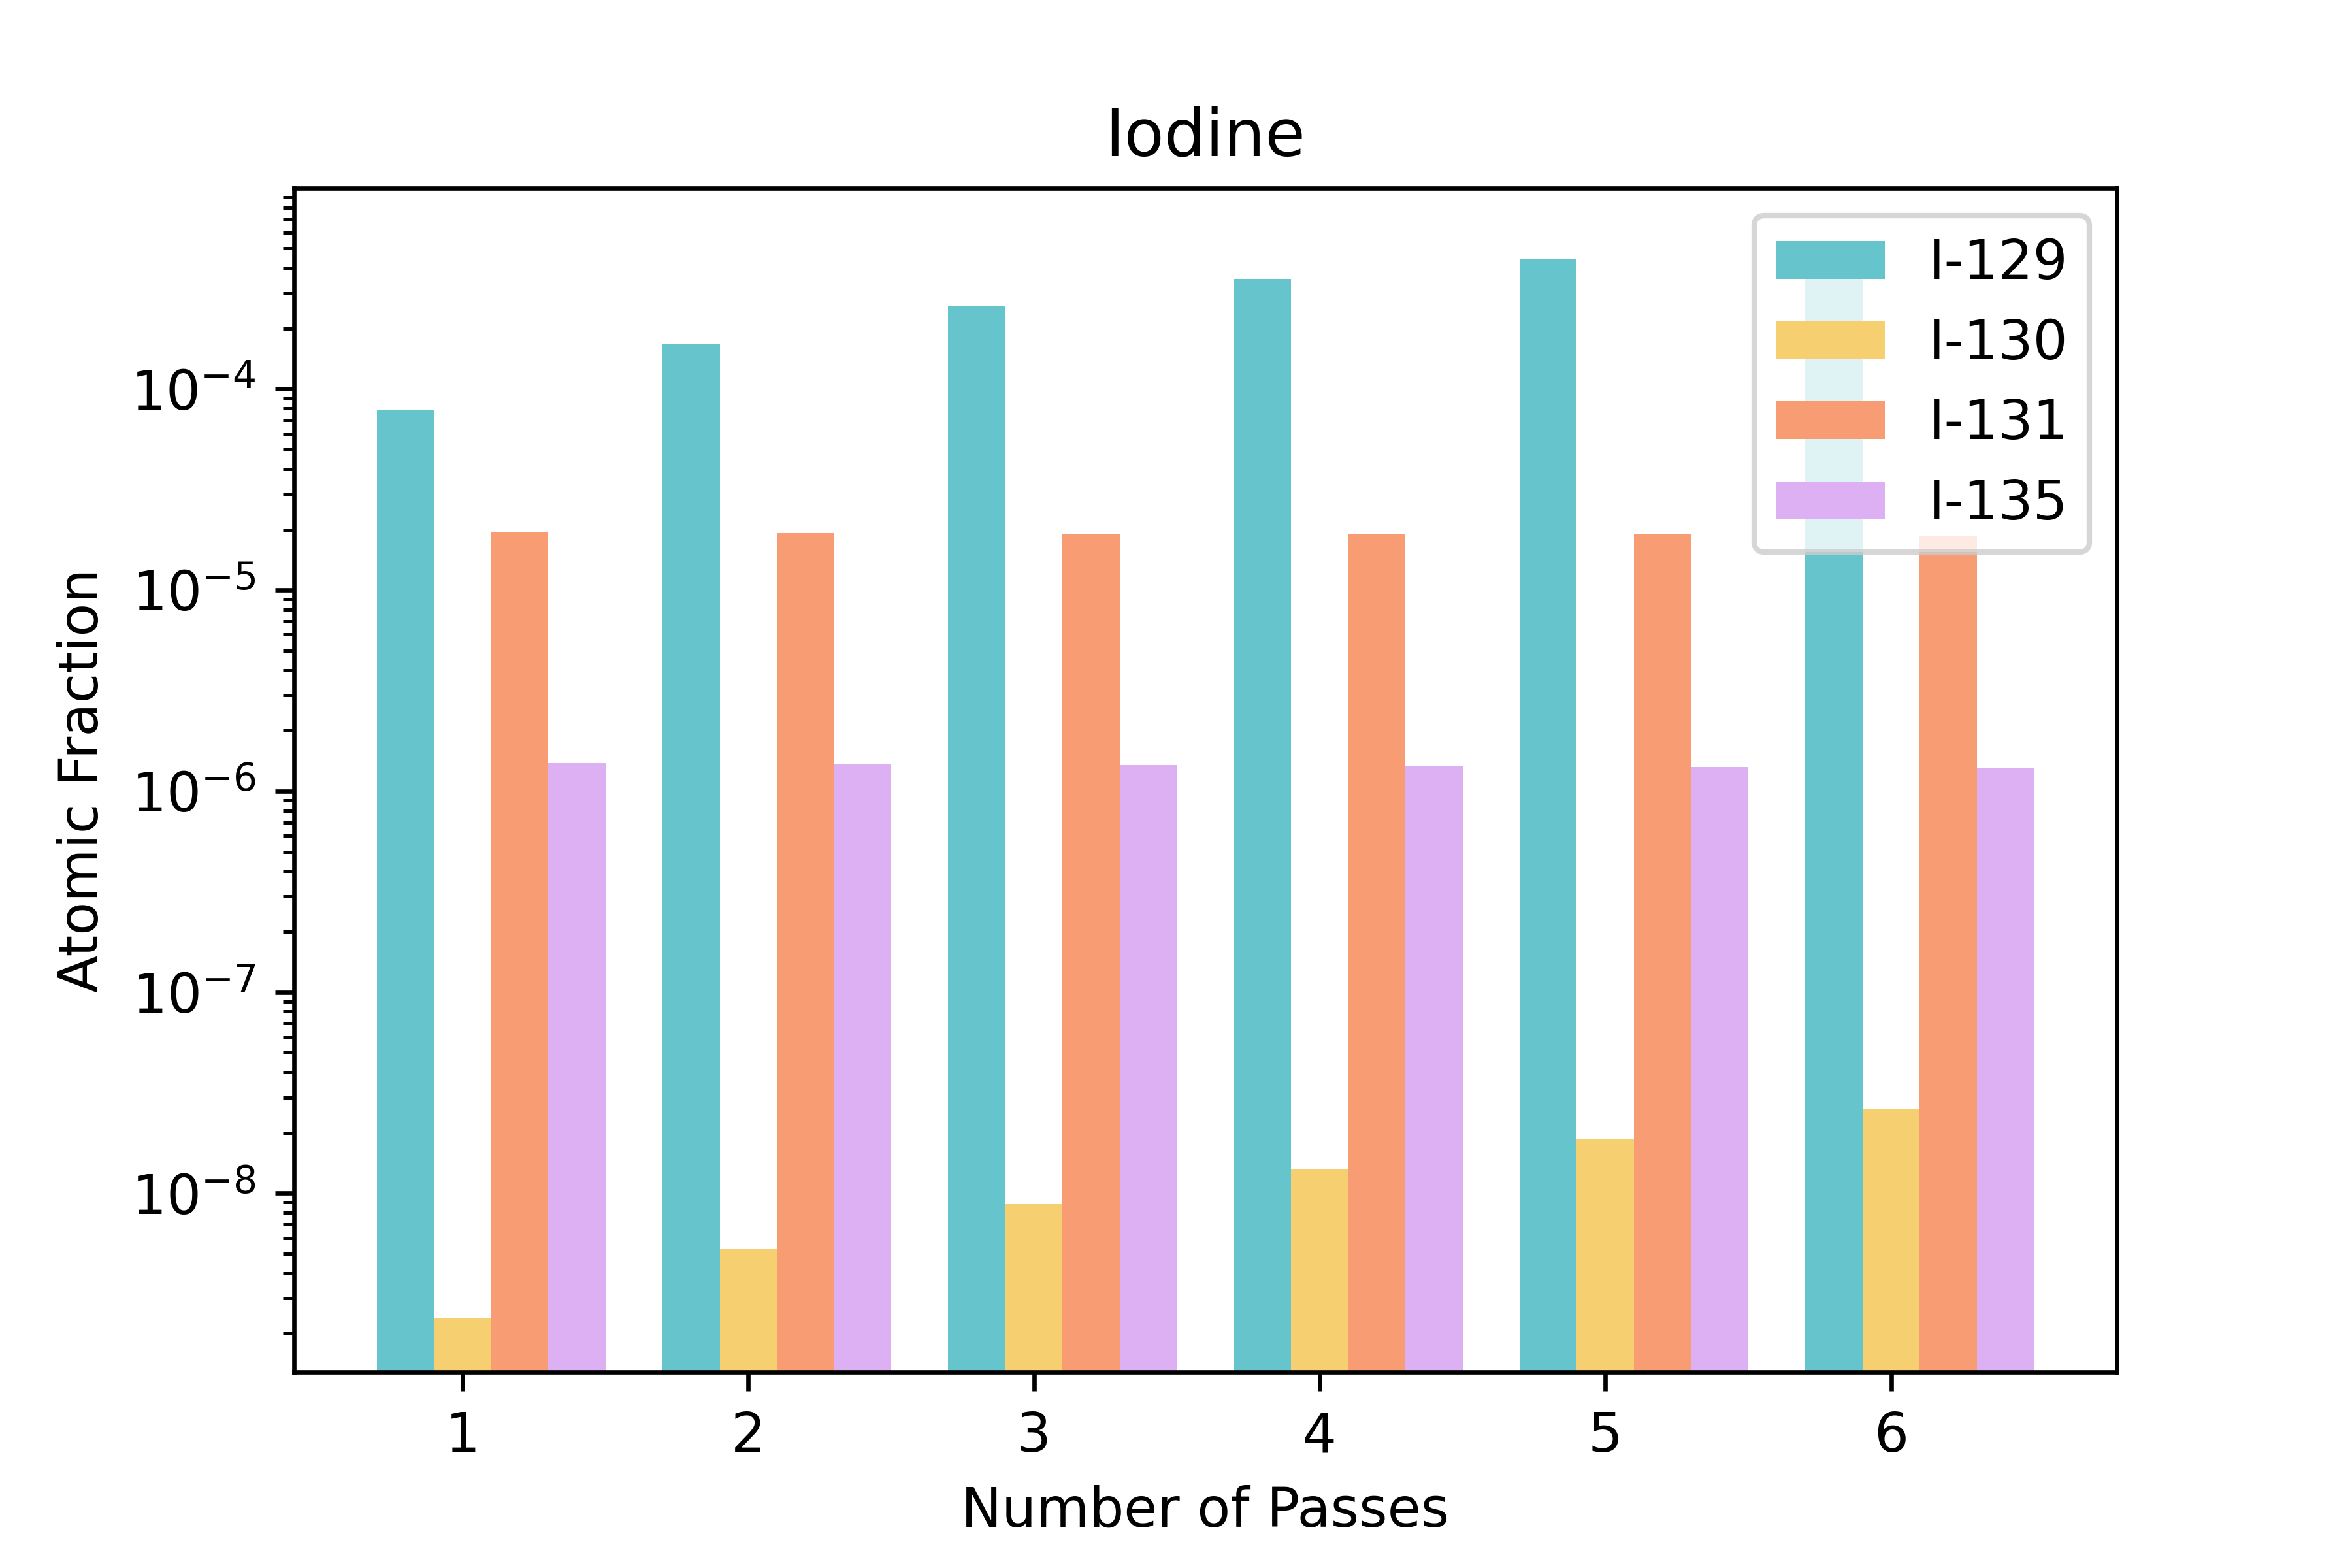
\includegraphics[width=\linewidth]{figures/compositions/iodine}
  \caption{Iodine isotope buildup over six burnup stages}
  \label{fig:i}
\end{subfigure}%

\begin{subfigure}{0.8\textwidth}
  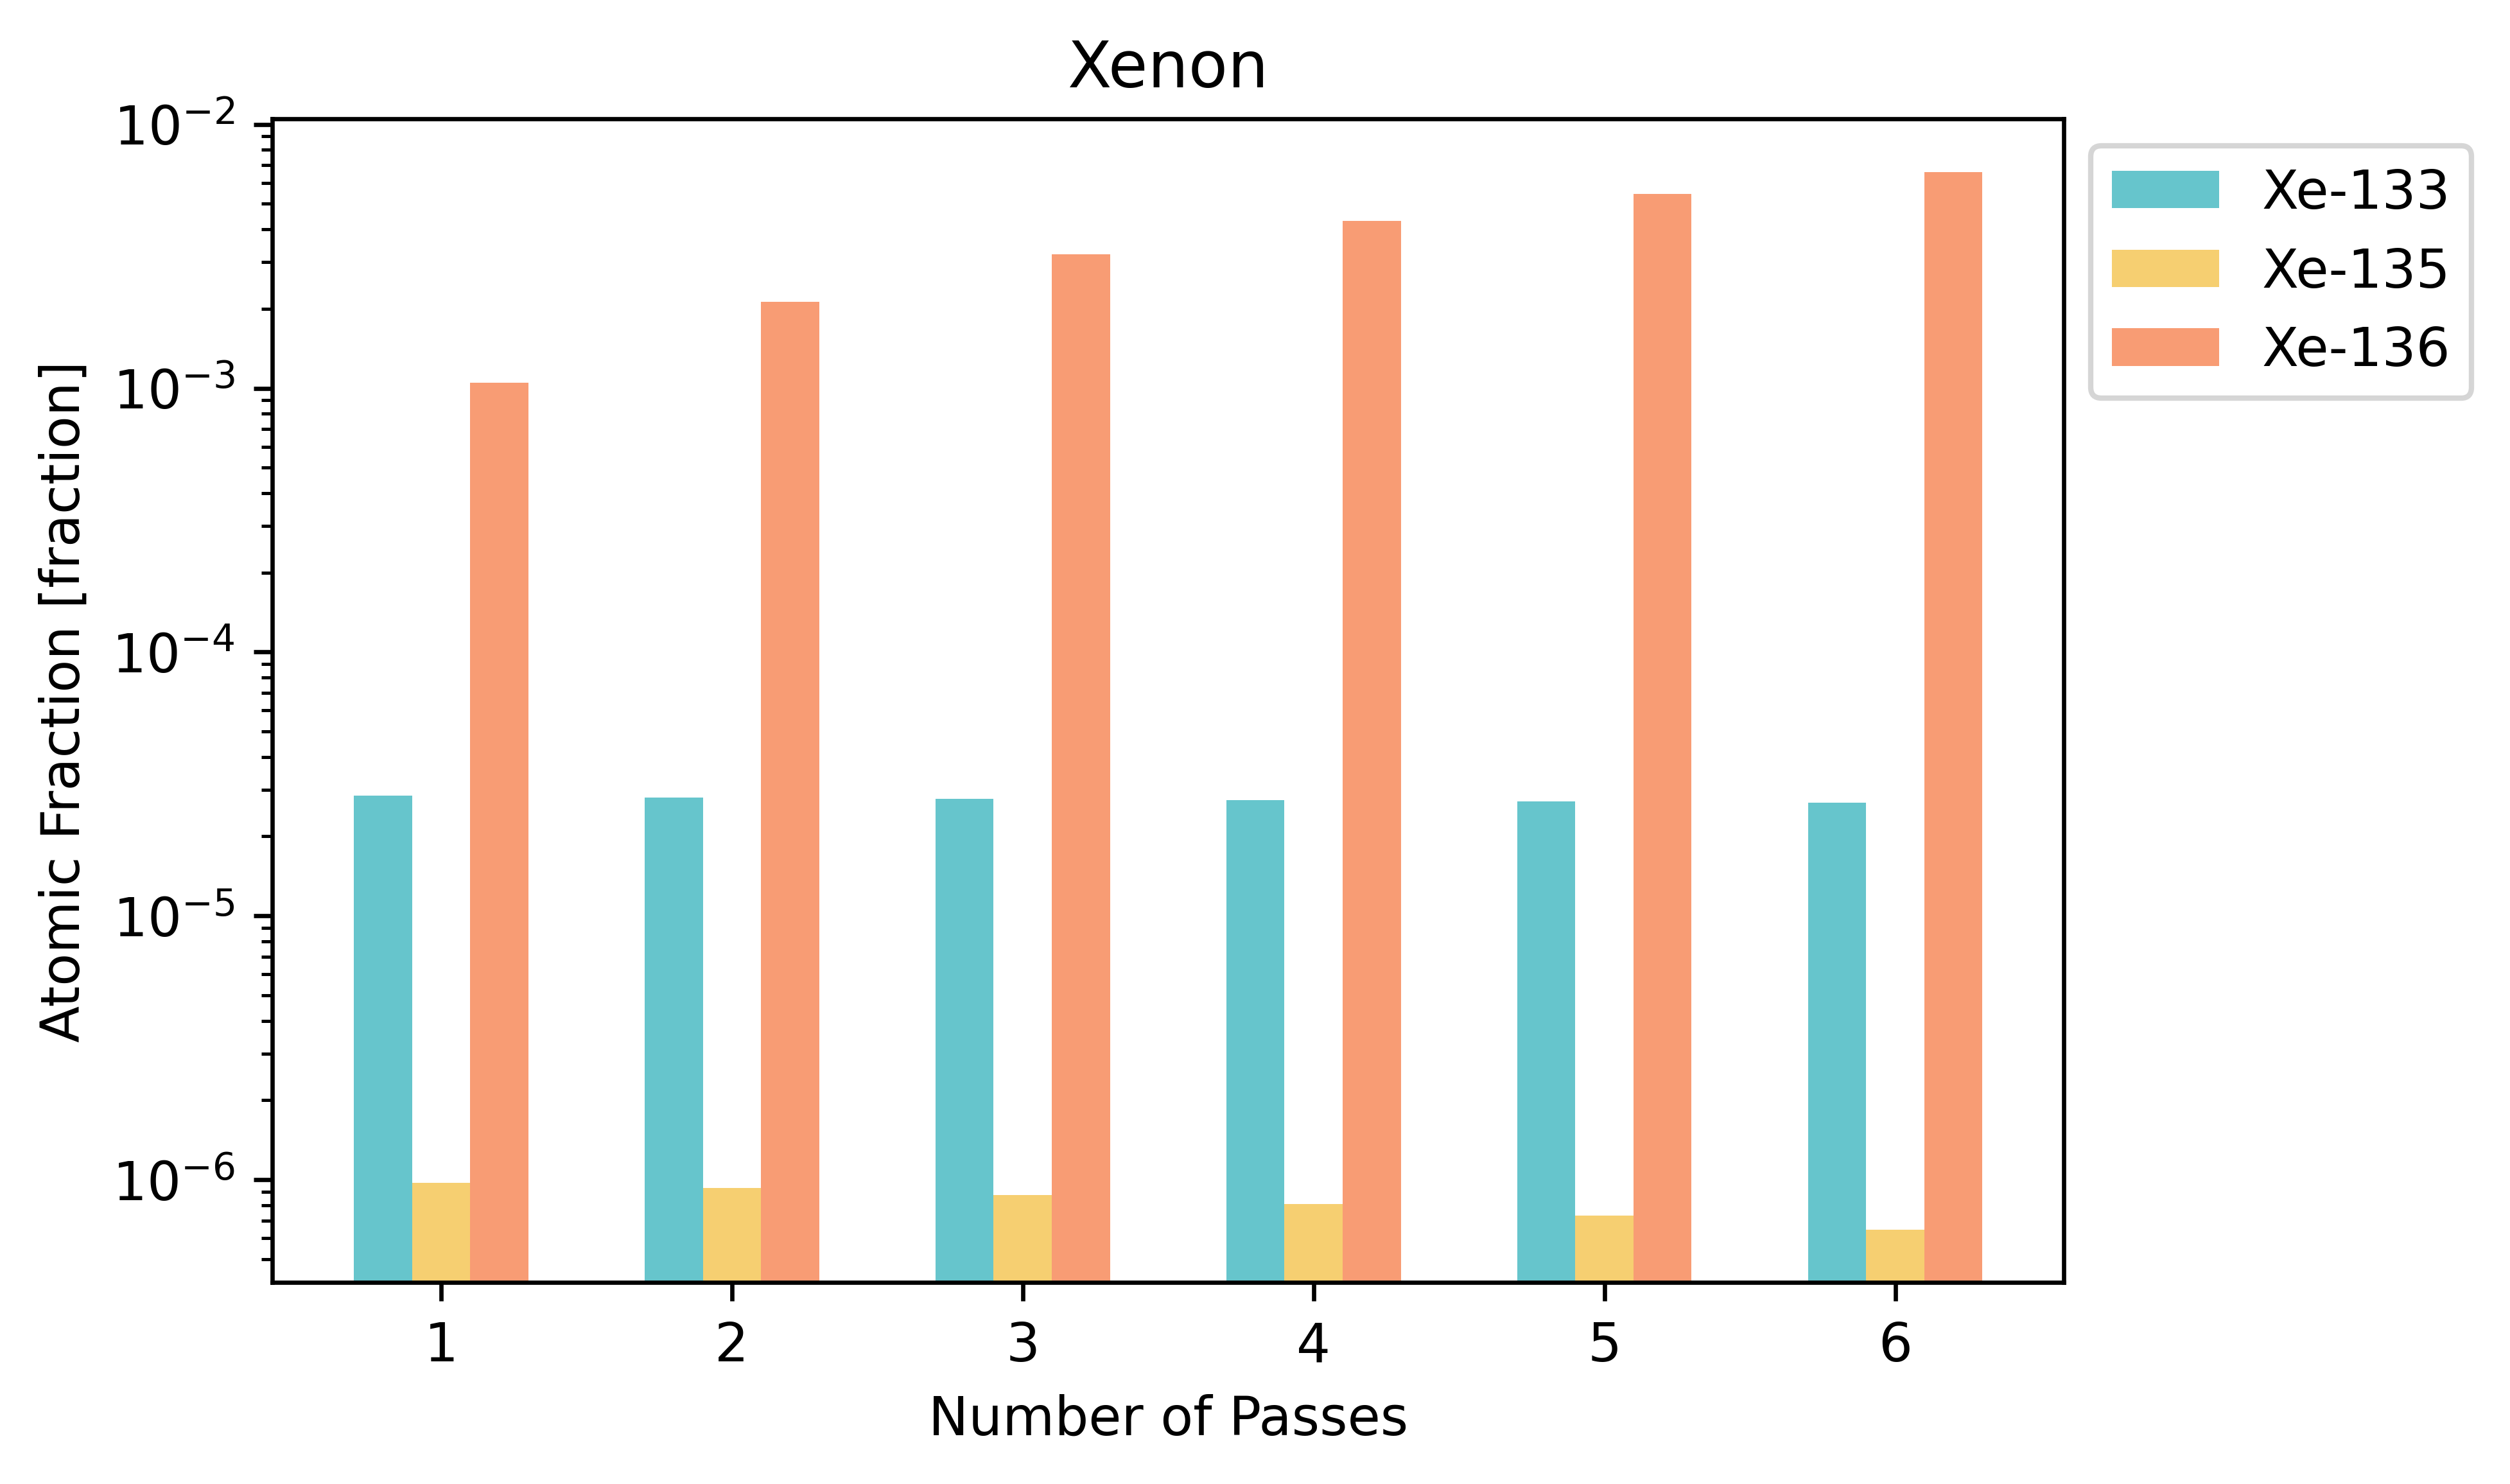
\includegraphics[width=\linewidth]{figures/compositions/xenon}
  \caption{Xenon isotope buildup over six burnup stages}
  \label{fig:xe}
\end{subfigure}%

\caption[Evolution of Safety Relevant Isotopic Concentrations in Pebbles of Sangamon20 over Six Six-Month Passes]{Evolution of Safety Relevant Isotopic Concentrations in Pebbles of Sangamon20 over Six Six-Month Passes (measured in atomic fraction)}
\end{figure}

\begin{figure}[H]\ContinuedFloat
\centering

\begin{subfigure}{0.8\textwidth}
  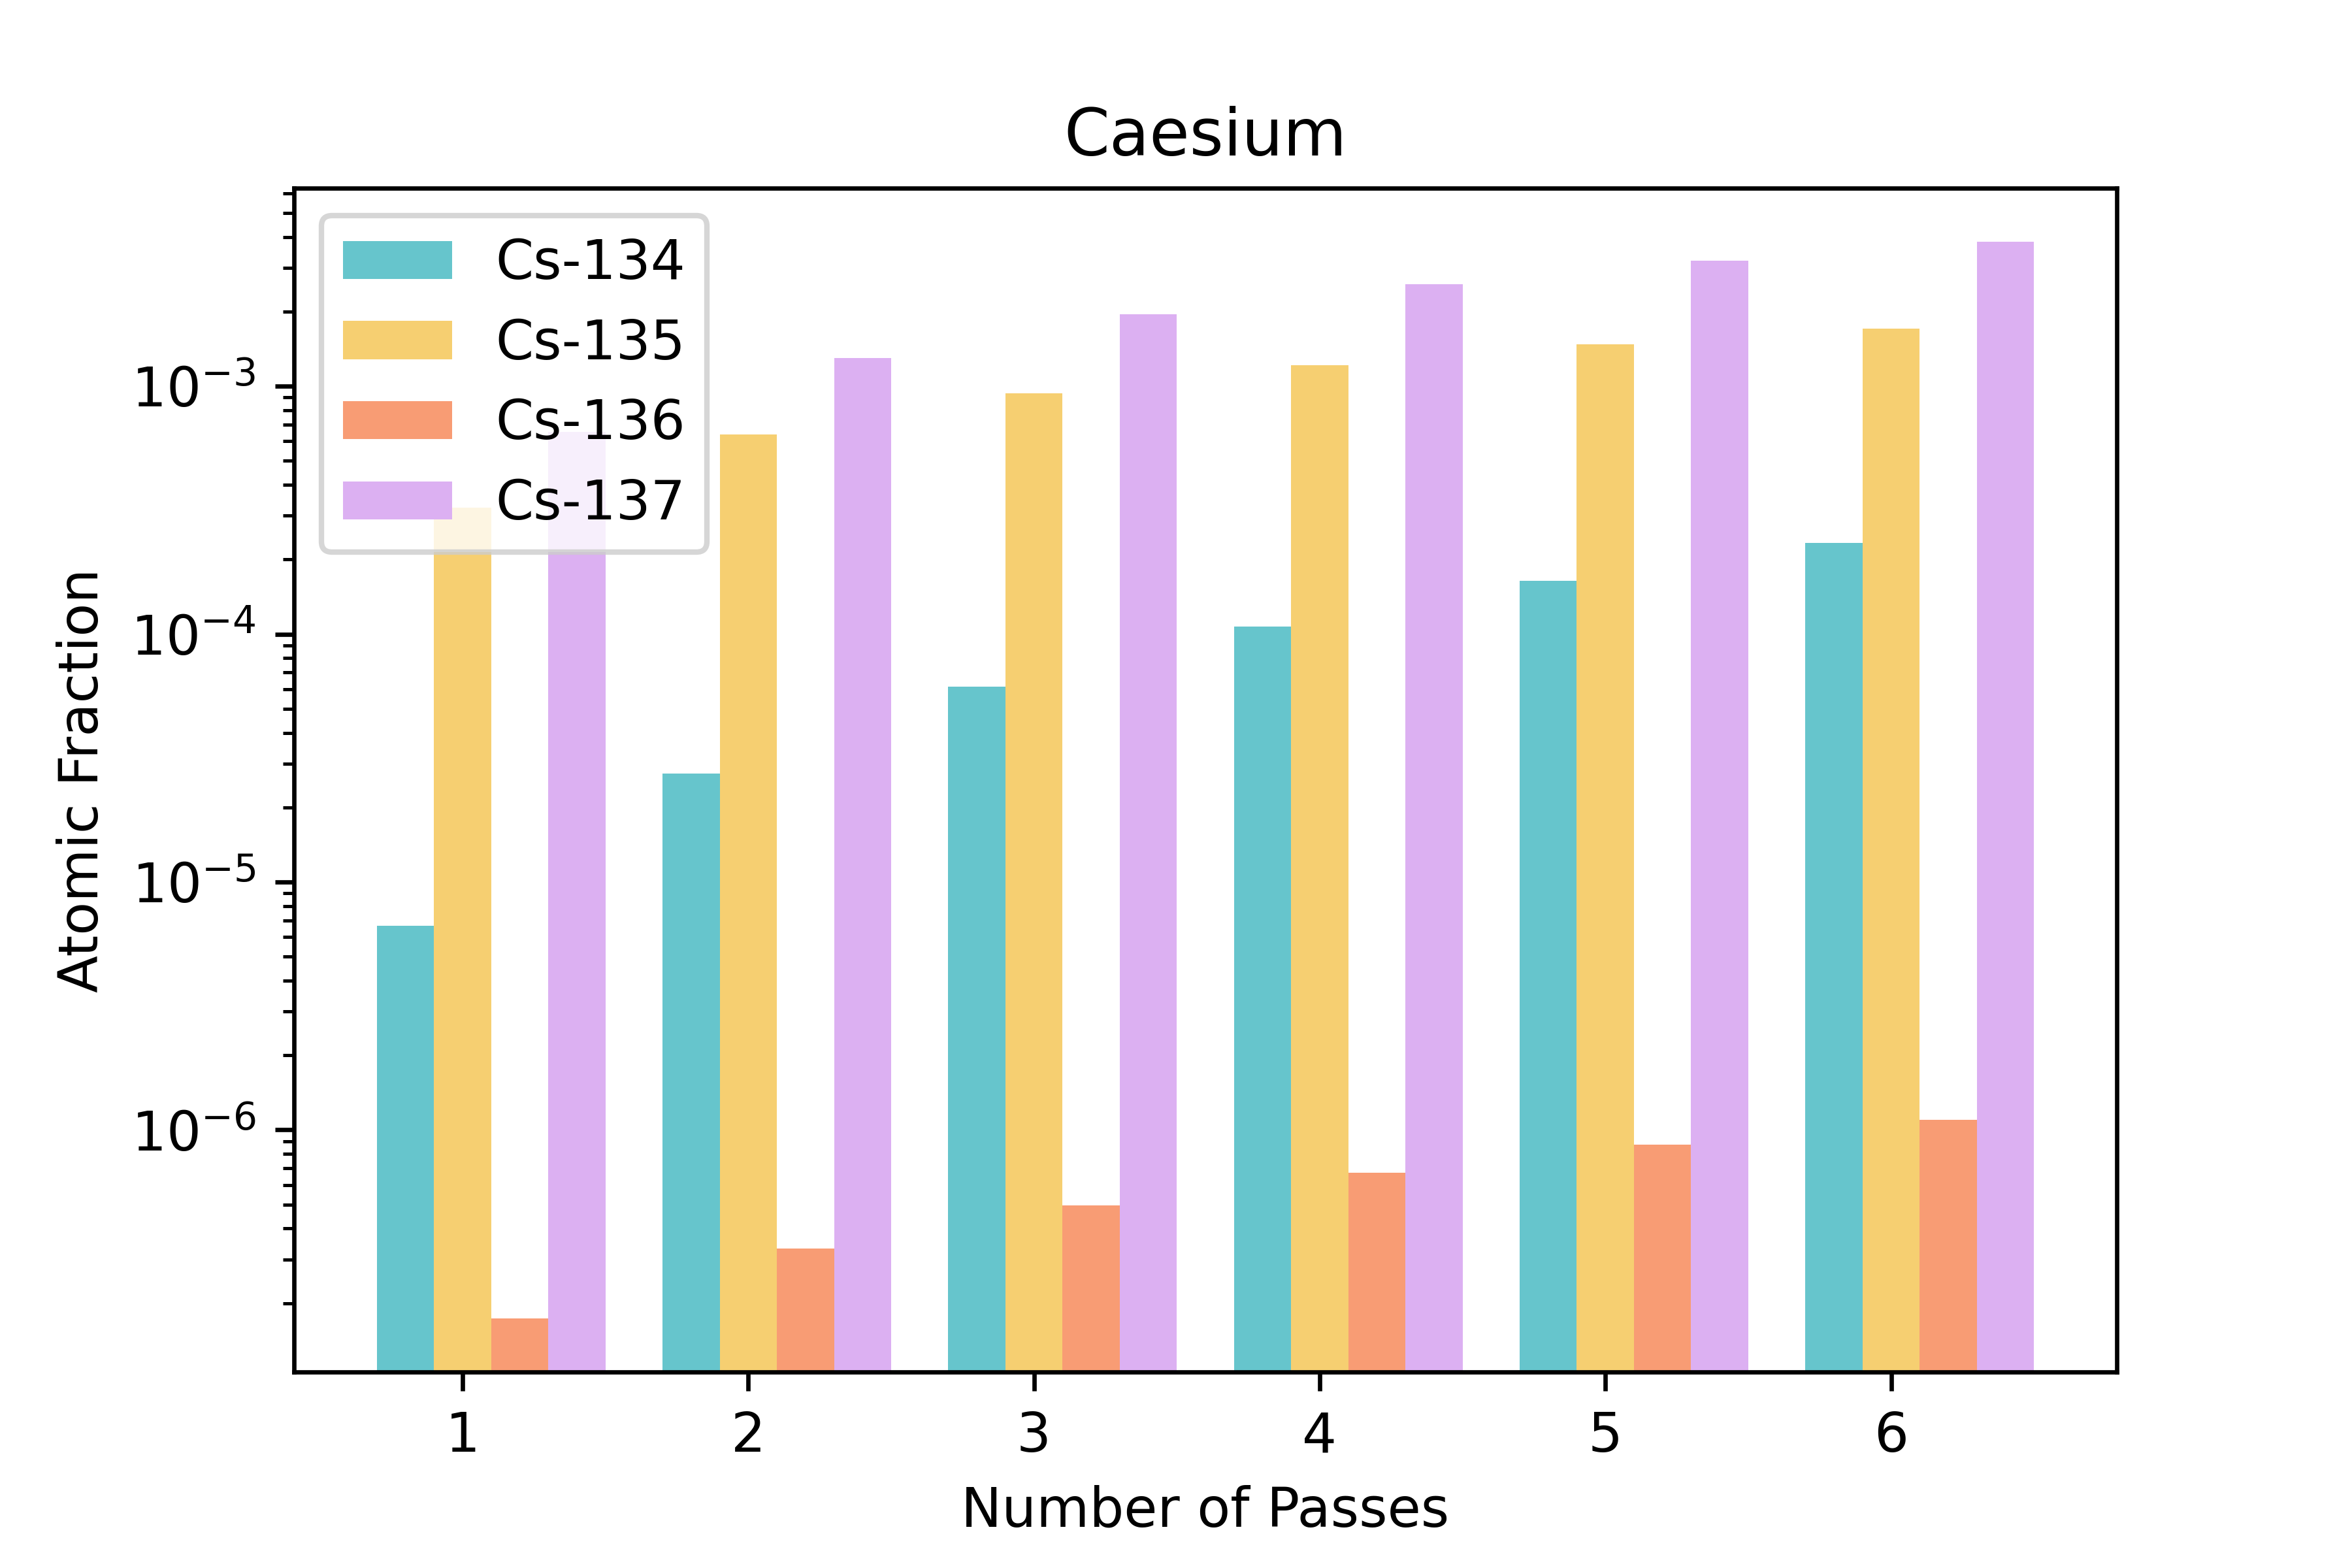
\includegraphics[width=\linewidth]{figures/compositions/caesium}
  \caption{Cesium isotope buildup over six burnup stages}
  \label{fig:cs}
\end{subfigure}%


\begin{subfigure}{0.8\textwidth}
  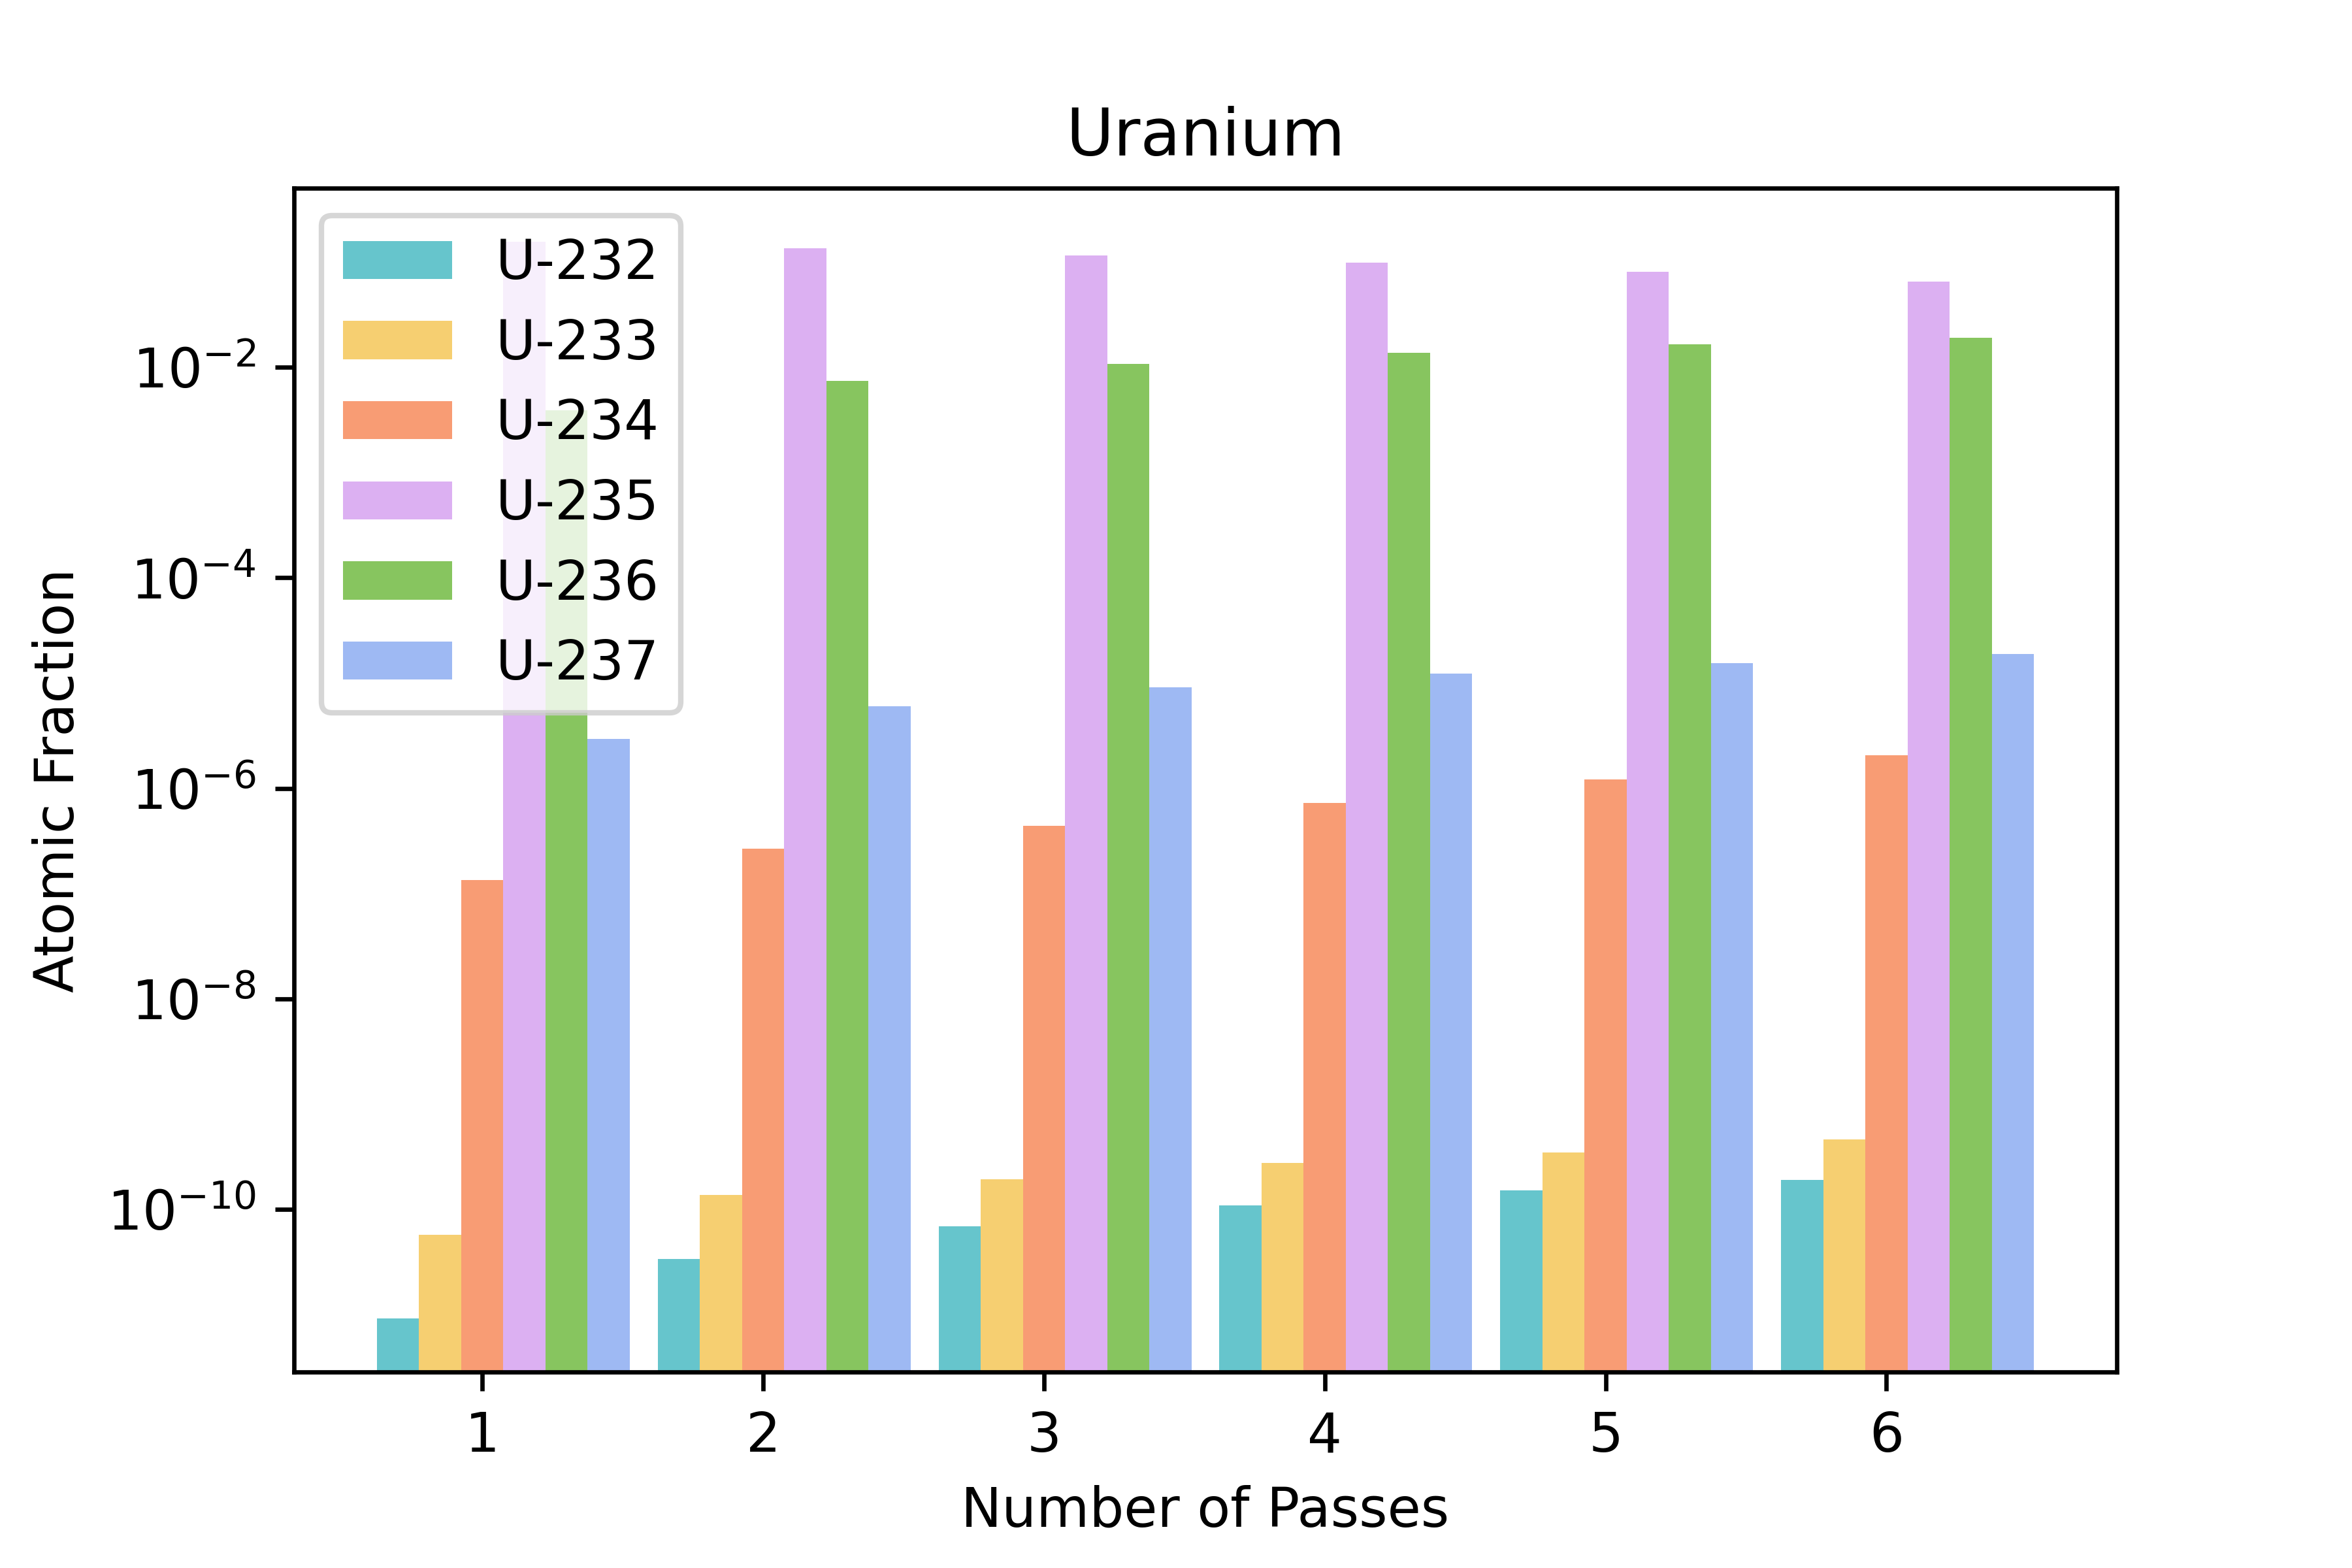
\includegraphics[width=\linewidth]{figures/compositions/uranium}
  \caption{Uranium isotope buildup over six burnup stages}
  \label{fig:u}
\end{subfigure}%

\caption[]{(cont.)}
\end{figure}

\begin{figure}[H]\ContinuedFloat
\centering

\begin{subfigure}{0.8\textwidth}
  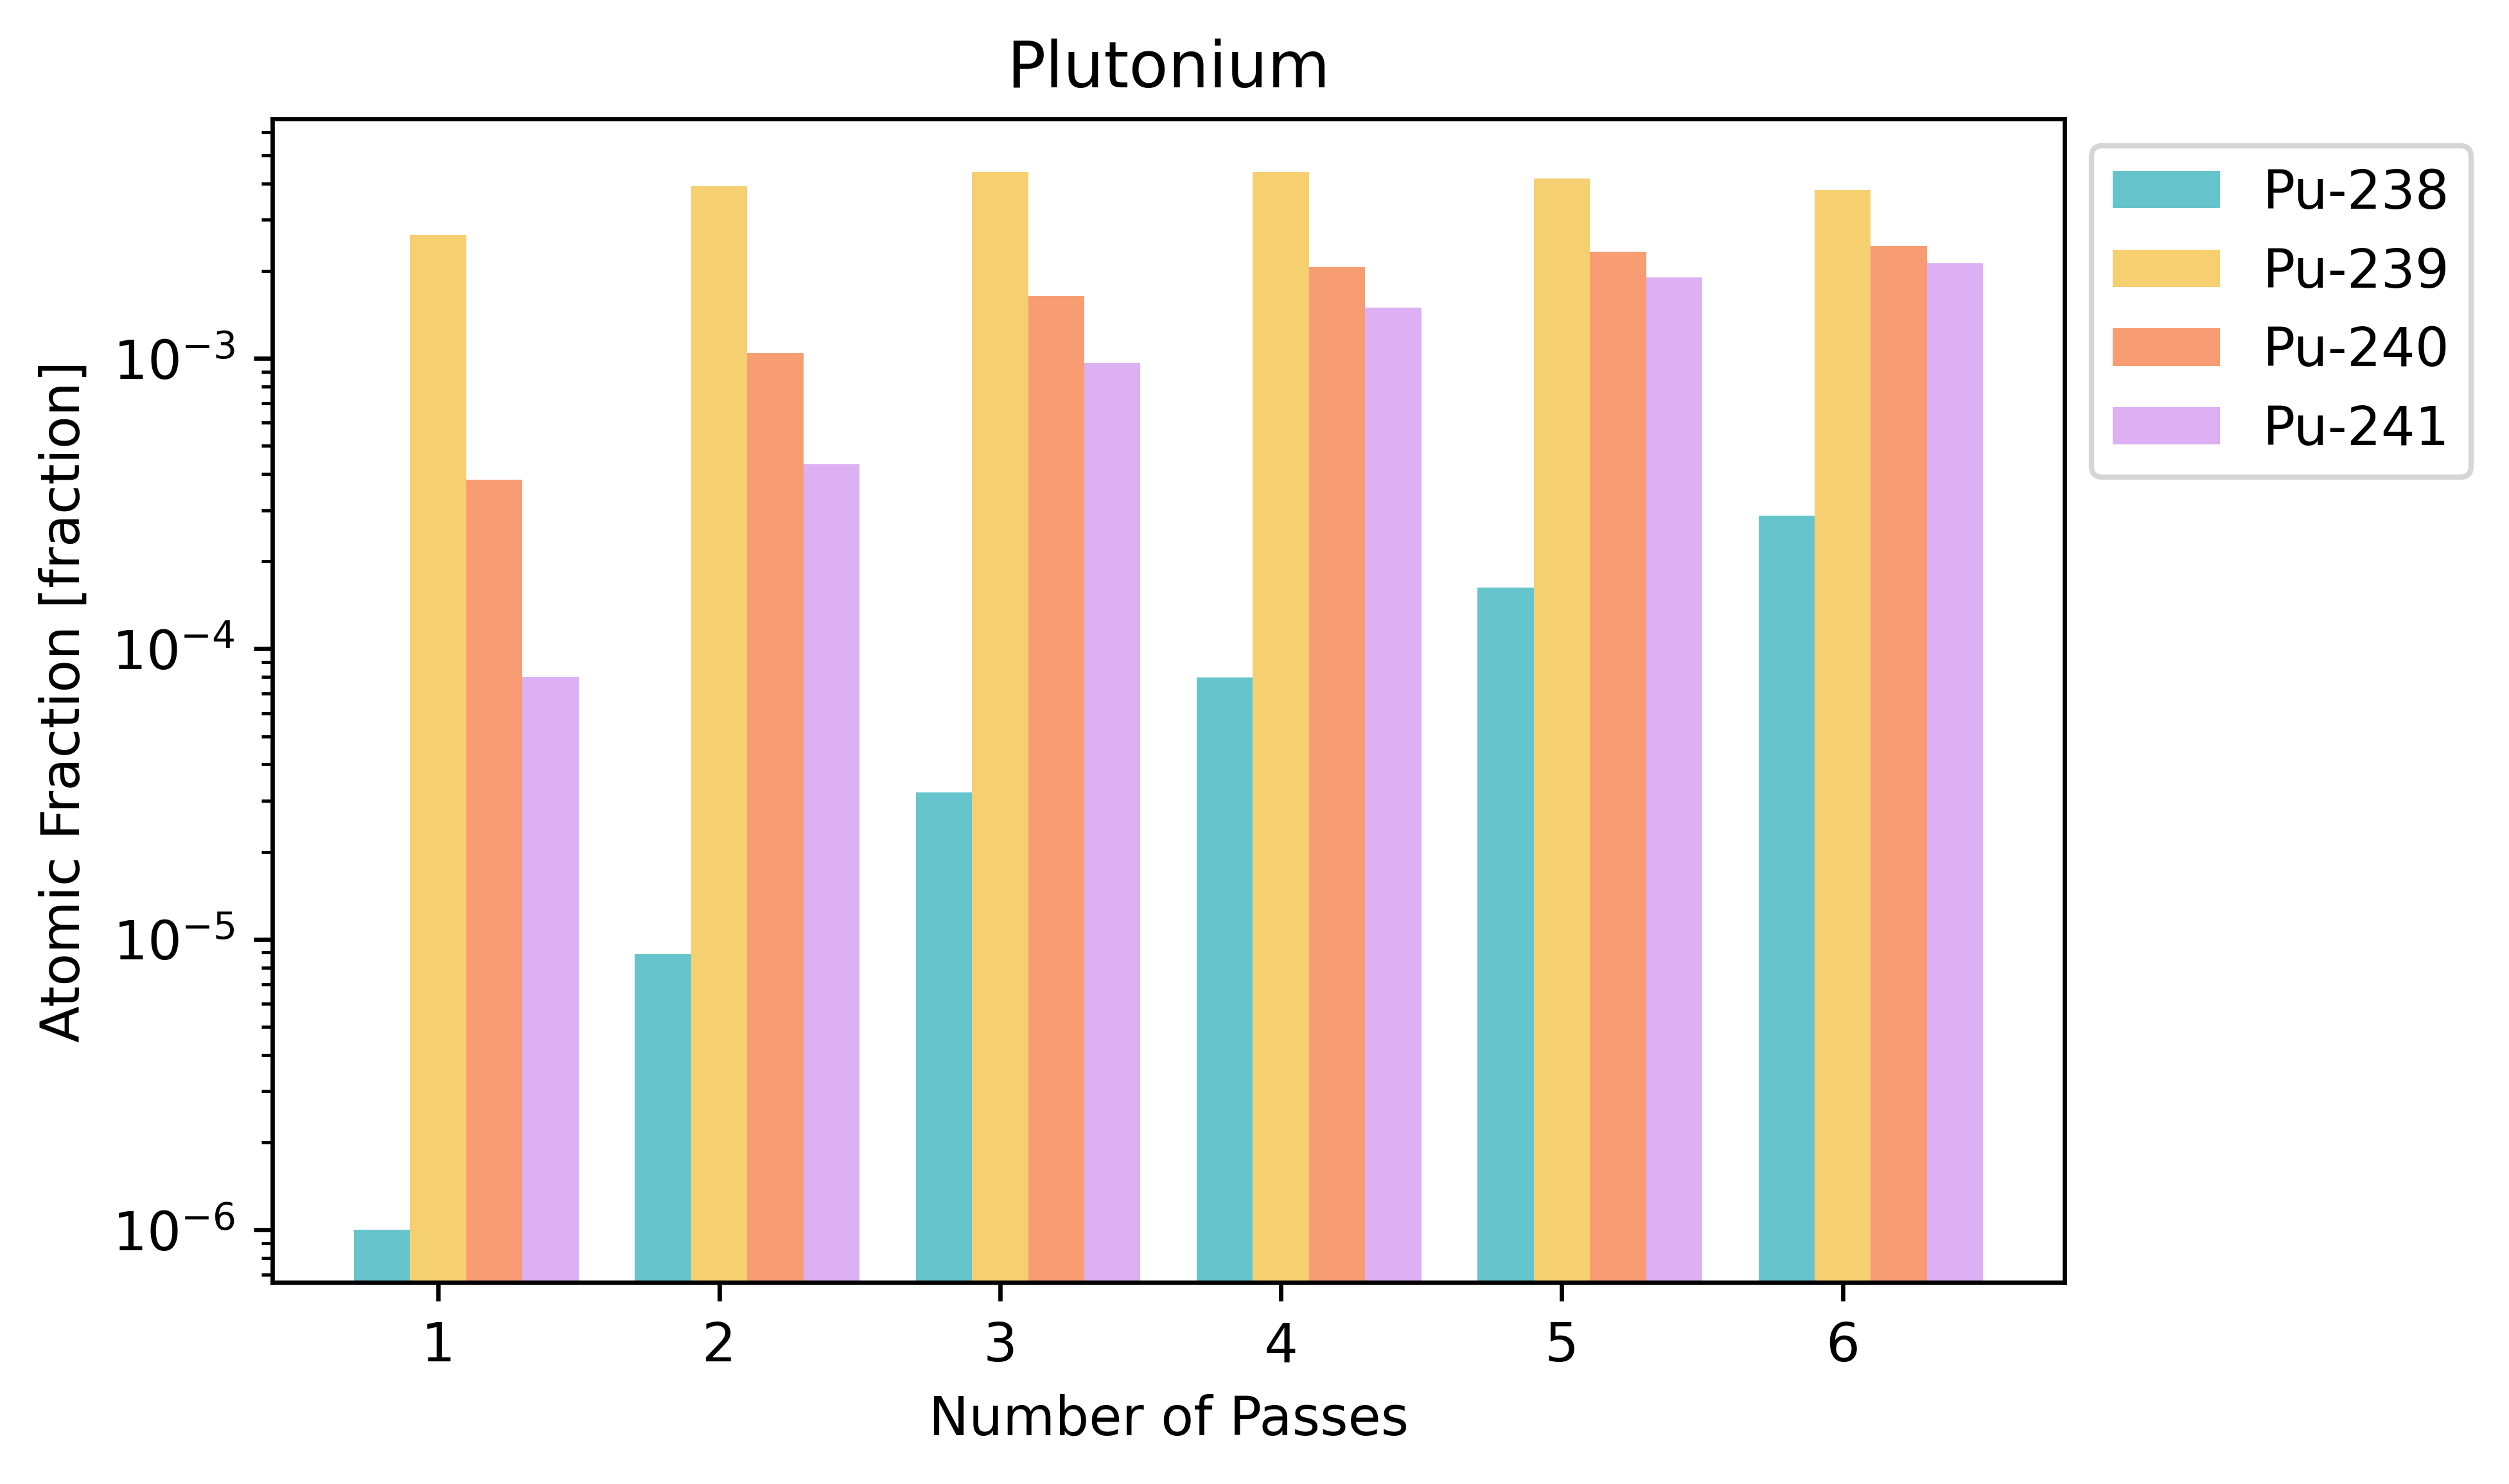
\includegraphics[width=\linewidth]{figures/compositions/plutonium}
  \caption{Plutonium isotope buildup over six burnup stages}
  \label{fig:pu}
\end{subfigure}%

\caption[]{(cont.)}
\label{fig:comps}
\end{figure}

The full isotopic inventory tracked in the Sangamon20 reactor models extends far beyond those supplied in Figure \ref{fig:comps}.  For a full list, see \cite{richter_isotopic_2021} for the compositions alone, or \cite{richter_zoerichterphlox_2021} for a complete input file and associated output.  Figure \ref{fig:comps} focuses on those of interest in safety analysis, such as those in Table \ref{table:dust-acc} and Table \ref{table:gas-acc}.

Only the xenon content rivals the inventory of uranium.  All isotopes of uranium steadily increase over time with the exception of $^{235}U$, ending at 0.0647 by atomic fraction in the sixth pass.  $^{232}U$, initially the smallest fraction of uranium sees the most dramatic increase over time, increasing by two orders of magnitude between the first ($9.28\times10^{-12}$) and sixth ($1.9\times10^{-10}$) cycle.  While the atomic fraction doesn't reach an equilibrium, the rate at which it increases each cycle is steady by the third pass - increasing by $4.02\times10^{-11}$,$4.2\times10^{-11}$, and $3.9\times10^{-11}$ from the third to fourth, fourth to fifth, and fifth to sixth pass, respectively.  Plutonium content is also fairly high, with $^{239}Pu$ peaking at 0.00439.  However, unlike many other isotopes, which peak in the sixth cycle, $^{239}Pu$ crests in the third and fourth passes, decreasing from 0.00439 in the fourth pass to 0.00380 in the sixth.  $^{238}Pu$, meanwhile, is the least abundant, but does experience the most dramatic increase over time (especially between the first and second passes).



$^{133}Xe$ appears to be steady around its initial concentration of $2.86\times10^{-05}$ atomic fraction, decreasing only to $2.68\times10^{-05}$ by the sixth pass.  $^{135}Xe$ decreases a bit more dramatically, going from an initial $9.70\times10^{-07}$ after its first six months, to  $6.46\times10^{-07}$ after thirty-six months.  $^{136}Xe$ is both the greatest contributor to xenon content in the fuel, and the only isotope reported in  Figure \ref{fig:xe} to increase, owing to its long half life.  Each cycle increases $^{136}Xe$ content by ~0.0011, beginning at a concentration of 0.00105 in the first cycle and ending at 0.0066 after the sixth.  Isotopes of iodine form a smaller portion of fission products than xenon or caesium (still a relatively high magnitude) which is of concern due to its high mobility in water and uptake in the thyroid.  $^{129}I$ is the most abundant isotope of iodine reported here.  It increases for the entirety of the pebble's life, beginning at $7.38\times10^{-05}$ and peaking at 0.000538 at its discharge burnup.  $^{130}I$ and $^{135}I$ are both relatively stable, most likely due to their short half-lives, combined with transmutation after undergoing neutron capture.  While $^{130}I$ is the least abundant, it increases over time.  Caesium has a net concentration similar to xenon's.  Unsurprisingly $^{135}Cs$ and $^{137}Cs$, which both have half-lives longer than a pebble's residency time in the reactor, are in greatest abundance, and increase over time.  These, too, are of concern, due to their long half-life.

Of the elements reported here, radium and thorium are in lowest abundance.  $^{225}Ra$ only appears in trace amounts (less than or equal to $9.99\times10^{-20}$) for the first three passes.  $^{224}Ra$ far outweighs the other reported isotopes of radium, with an atomic fraction of $7.46\times10^{-15}$ after thirty-six months - two orders of magnitude higher than all other isotopes of radium combined at this depletion step.  Thorium has the second-least abundant atomic fractions, with fertile $^{232}Th$ being the most abundant, at $8.80\times10^{-10}$ in the sixth pass.  However, being present only in low concentrations is not enough to ensure that it is not a risk in an accident scenario.  An isotope with a very short half-life, or ones that are toxic in addition to being radioactive can pose a serious threat even in relatively low amounts.

\section{Full-Core Control Model}
\label{res-control}

Figure \ref{fig:controlmain} shows a cross section of the core geometry at the origin (the midplane, the center of which is the point (0, 0, 0) ) in the xy and xz planes (Sub-Figures \ref{fig:controla} and \ref{fig:controlc}, respectively) and provides a mesh of the fission rate and thermal flux in the xy and xz planes (Sub-Figures \ref{fig:controlb} and \ref{fig:controld}, respectively).  Both of these integrate over z and y, respectively, to produce a 2D image.  The value of $k_{eff}$ was $1.041 \pm 0.00054$.

Figure \ref{fig:geom-legend1} is accurate for all cross sections of reactor geometry.  In homogenized simulations, the shades of green represent the material blend forming the center of the pebble at a given burnup.  For heterogenized simulations, these same shades represent the TRISO particle kernel at a particular burnup.

\begin{figure}[H]
\centering

\begin{subfigure}{0.45\textwidth}
  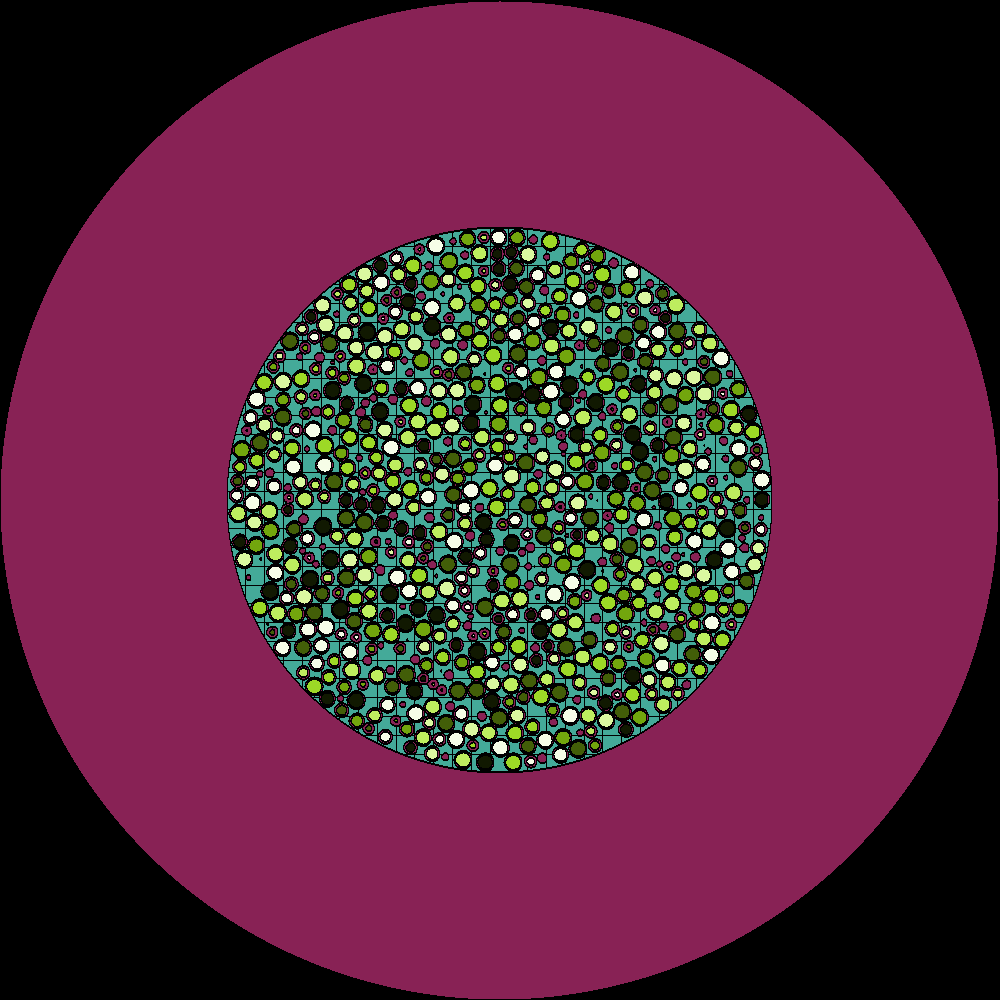
\includegraphics[width=0.95\linewidth]{figures/control/control-r}
  \caption{Radial Cross Section at y=0}
  \label{fig:controla}
\end{subfigure}%
%
\begin{subfigure}{0.45\textwidth}
  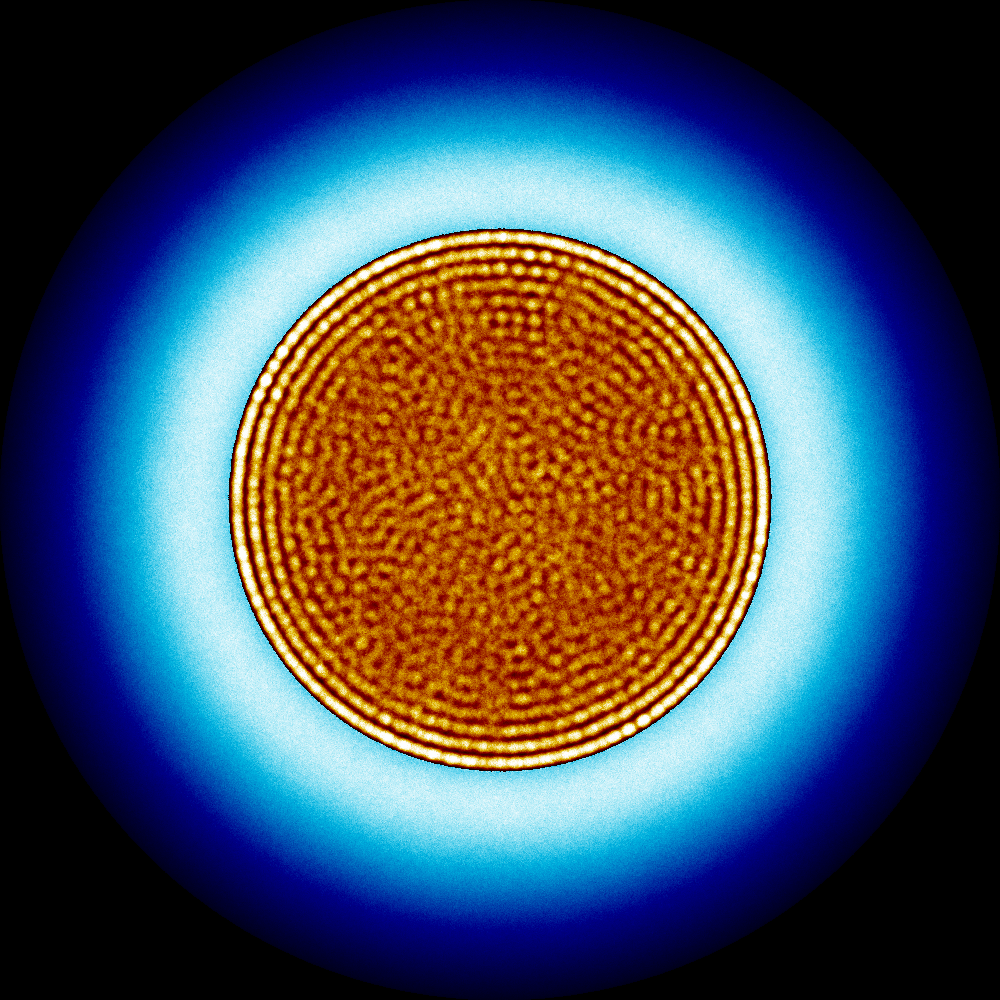
\includegraphics[width=0.95\linewidth]{figures/control/control-rm}
  \caption{Radial Mesh}
  \label{fig:controlb}
\end{subfigure}

\begin{subfigure}{0.45\textwidth}
  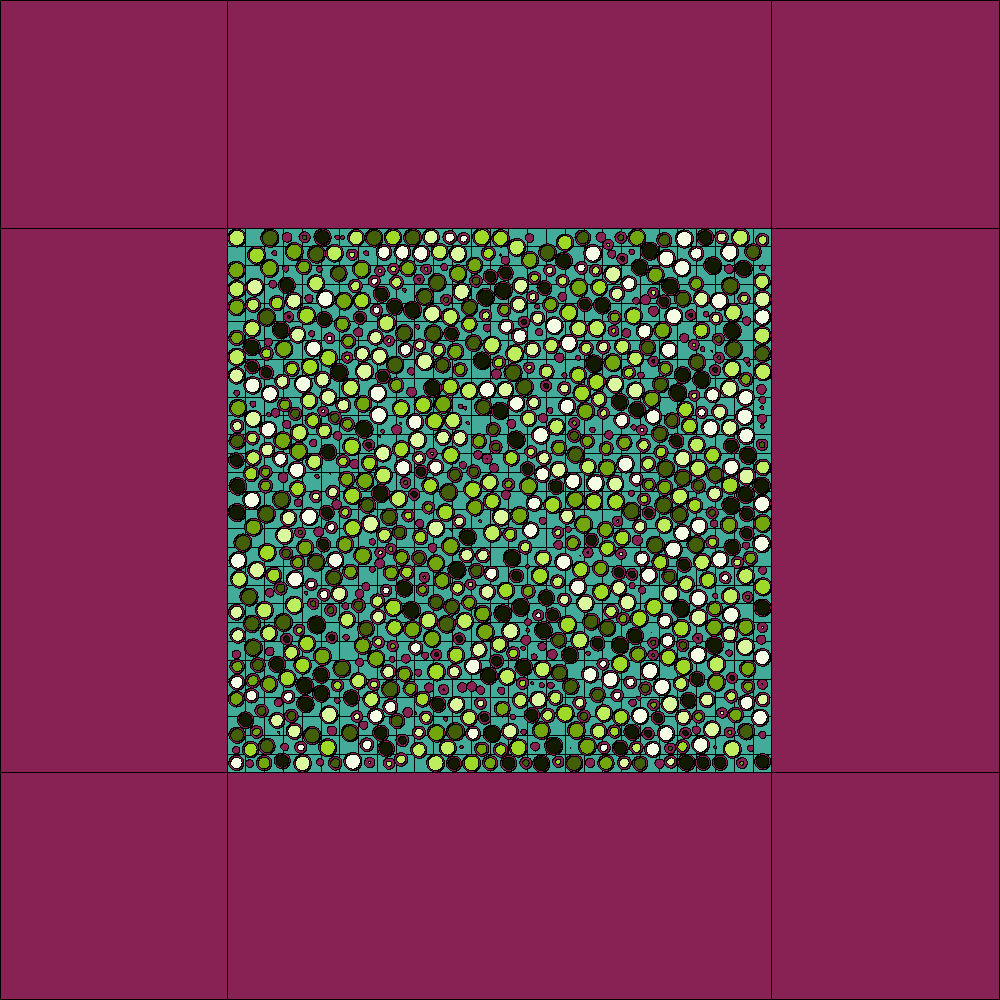
\includegraphics[width=0.95\linewidth]{figures/control/control-v}
  \caption{Axial Cross Section at z=0 }
  \label{fig:controlc}
\end{subfigure}
%
\begin{subfigure}{0.45\textwidth}
  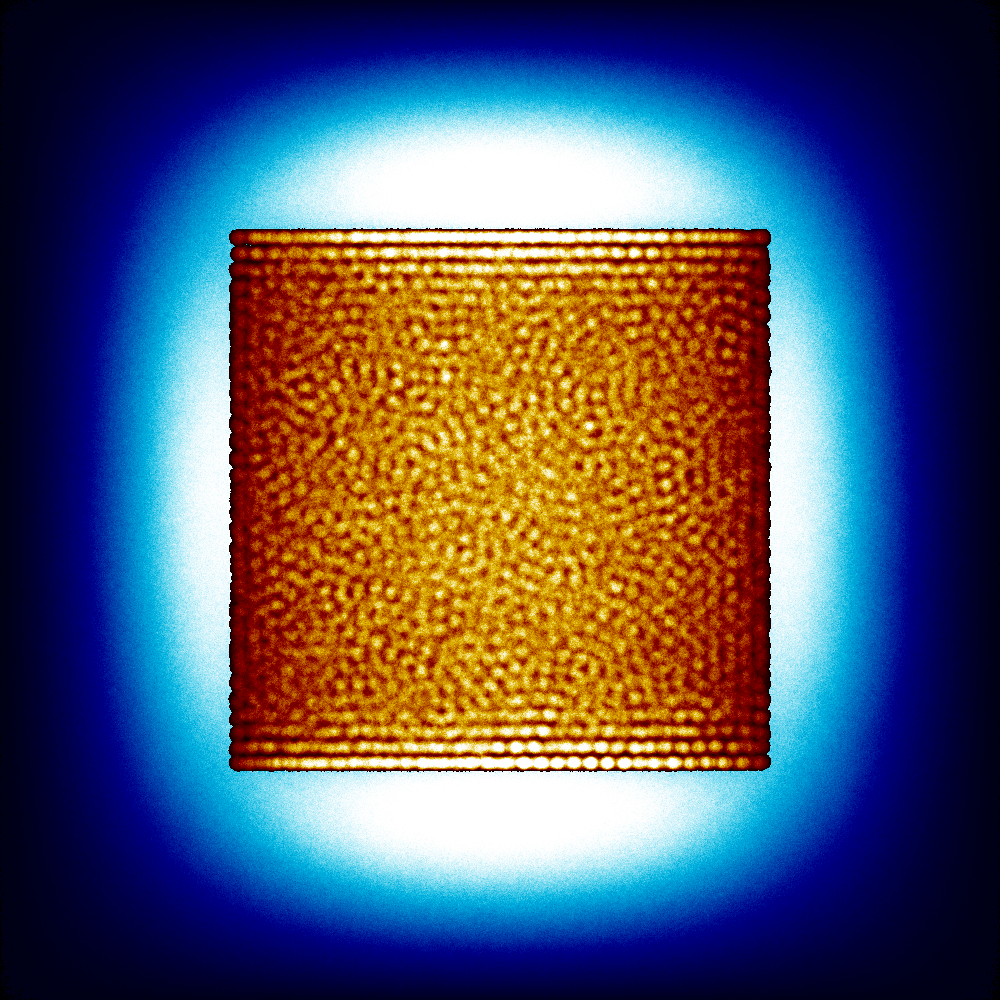
\includegraphics[width=0.95\linewidth]{figures/control/control-vm}
  \caption{Axial Mesh}
  \label{fig:controld}
\end{subfigure}
%
\begin{subfigure}{\textwidth}
\centering
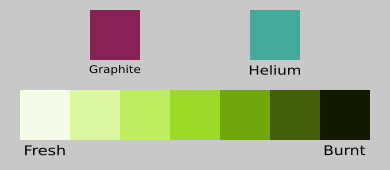
\includegraphics[width=0.6\linewidth]{figures/geom-legend}
\caption{Legend for \ref{fig:controla} and \ref{fig:controlc}}
\label{fig:geom-legend1}
\end{subfigure}

\caption{Geometry Cross Sections (left) and Thermal Flux(cold color map) and Fission Rate (hot color map) Meshes (right) for the Control Model of Sangamon20}
\label{fig:controlmain}
\end{figure}

Figure \ref{fig:controlb} shows bands of concentric rings around the outer edges of the active core.  These bands suggest that the outermost areas of the core are regions of high fission activity relative to the center, which is at odds with what most might expect from the neutronics behavior in a cylindrical reactor.  Certainly the pebbles are physically forming rings at the outer edges, and their placement becomes less structured toward the center.  However, the high intensities seen in this outer region in the mesh figures are unindicative of a total flux profile showing the same.  Recall that Serpent integrates over the z direction to produce a 2D plot of the xy plane.  For a cylinder, the distance in z each point integrates over is the same - the height of the reactor.  However, points at the outermost regions are integrating in a volume composed more of pebbles - and therefore fissile material - than the center, where more space filled with coolant.  The outer regions are more regularly packed with pebbles - and therefore have less coolant than the center - because the dispersal routine (and the grow and shake algorithm) naturally cause the pebbles to line up along the reactor boundary.  Lattice arrangements wouldn't have this feature because these methods ignore core boundaries.

In Figure \ref{fig:controld} we can see a similar banding effect on the top and bottom edge of the core region, but not on the sides.  No hot-spots on the edges because Figure \ref{fig:controld} is in the xz plane, and integrates over y.  However, for a cylinder, the distance integrated over is not the same at all points.  At the centerline, the distance is simply the diameter.  However, as you move towards the edge, the distance integrated over approaches zero.  So, while these plots can help provide some insight into the core, one must be very careful to keep this uneven integration in mind when interpreting them.

\begin{figure}[H]
\centering

\begin{subfigure}{0.9\textwidth}
  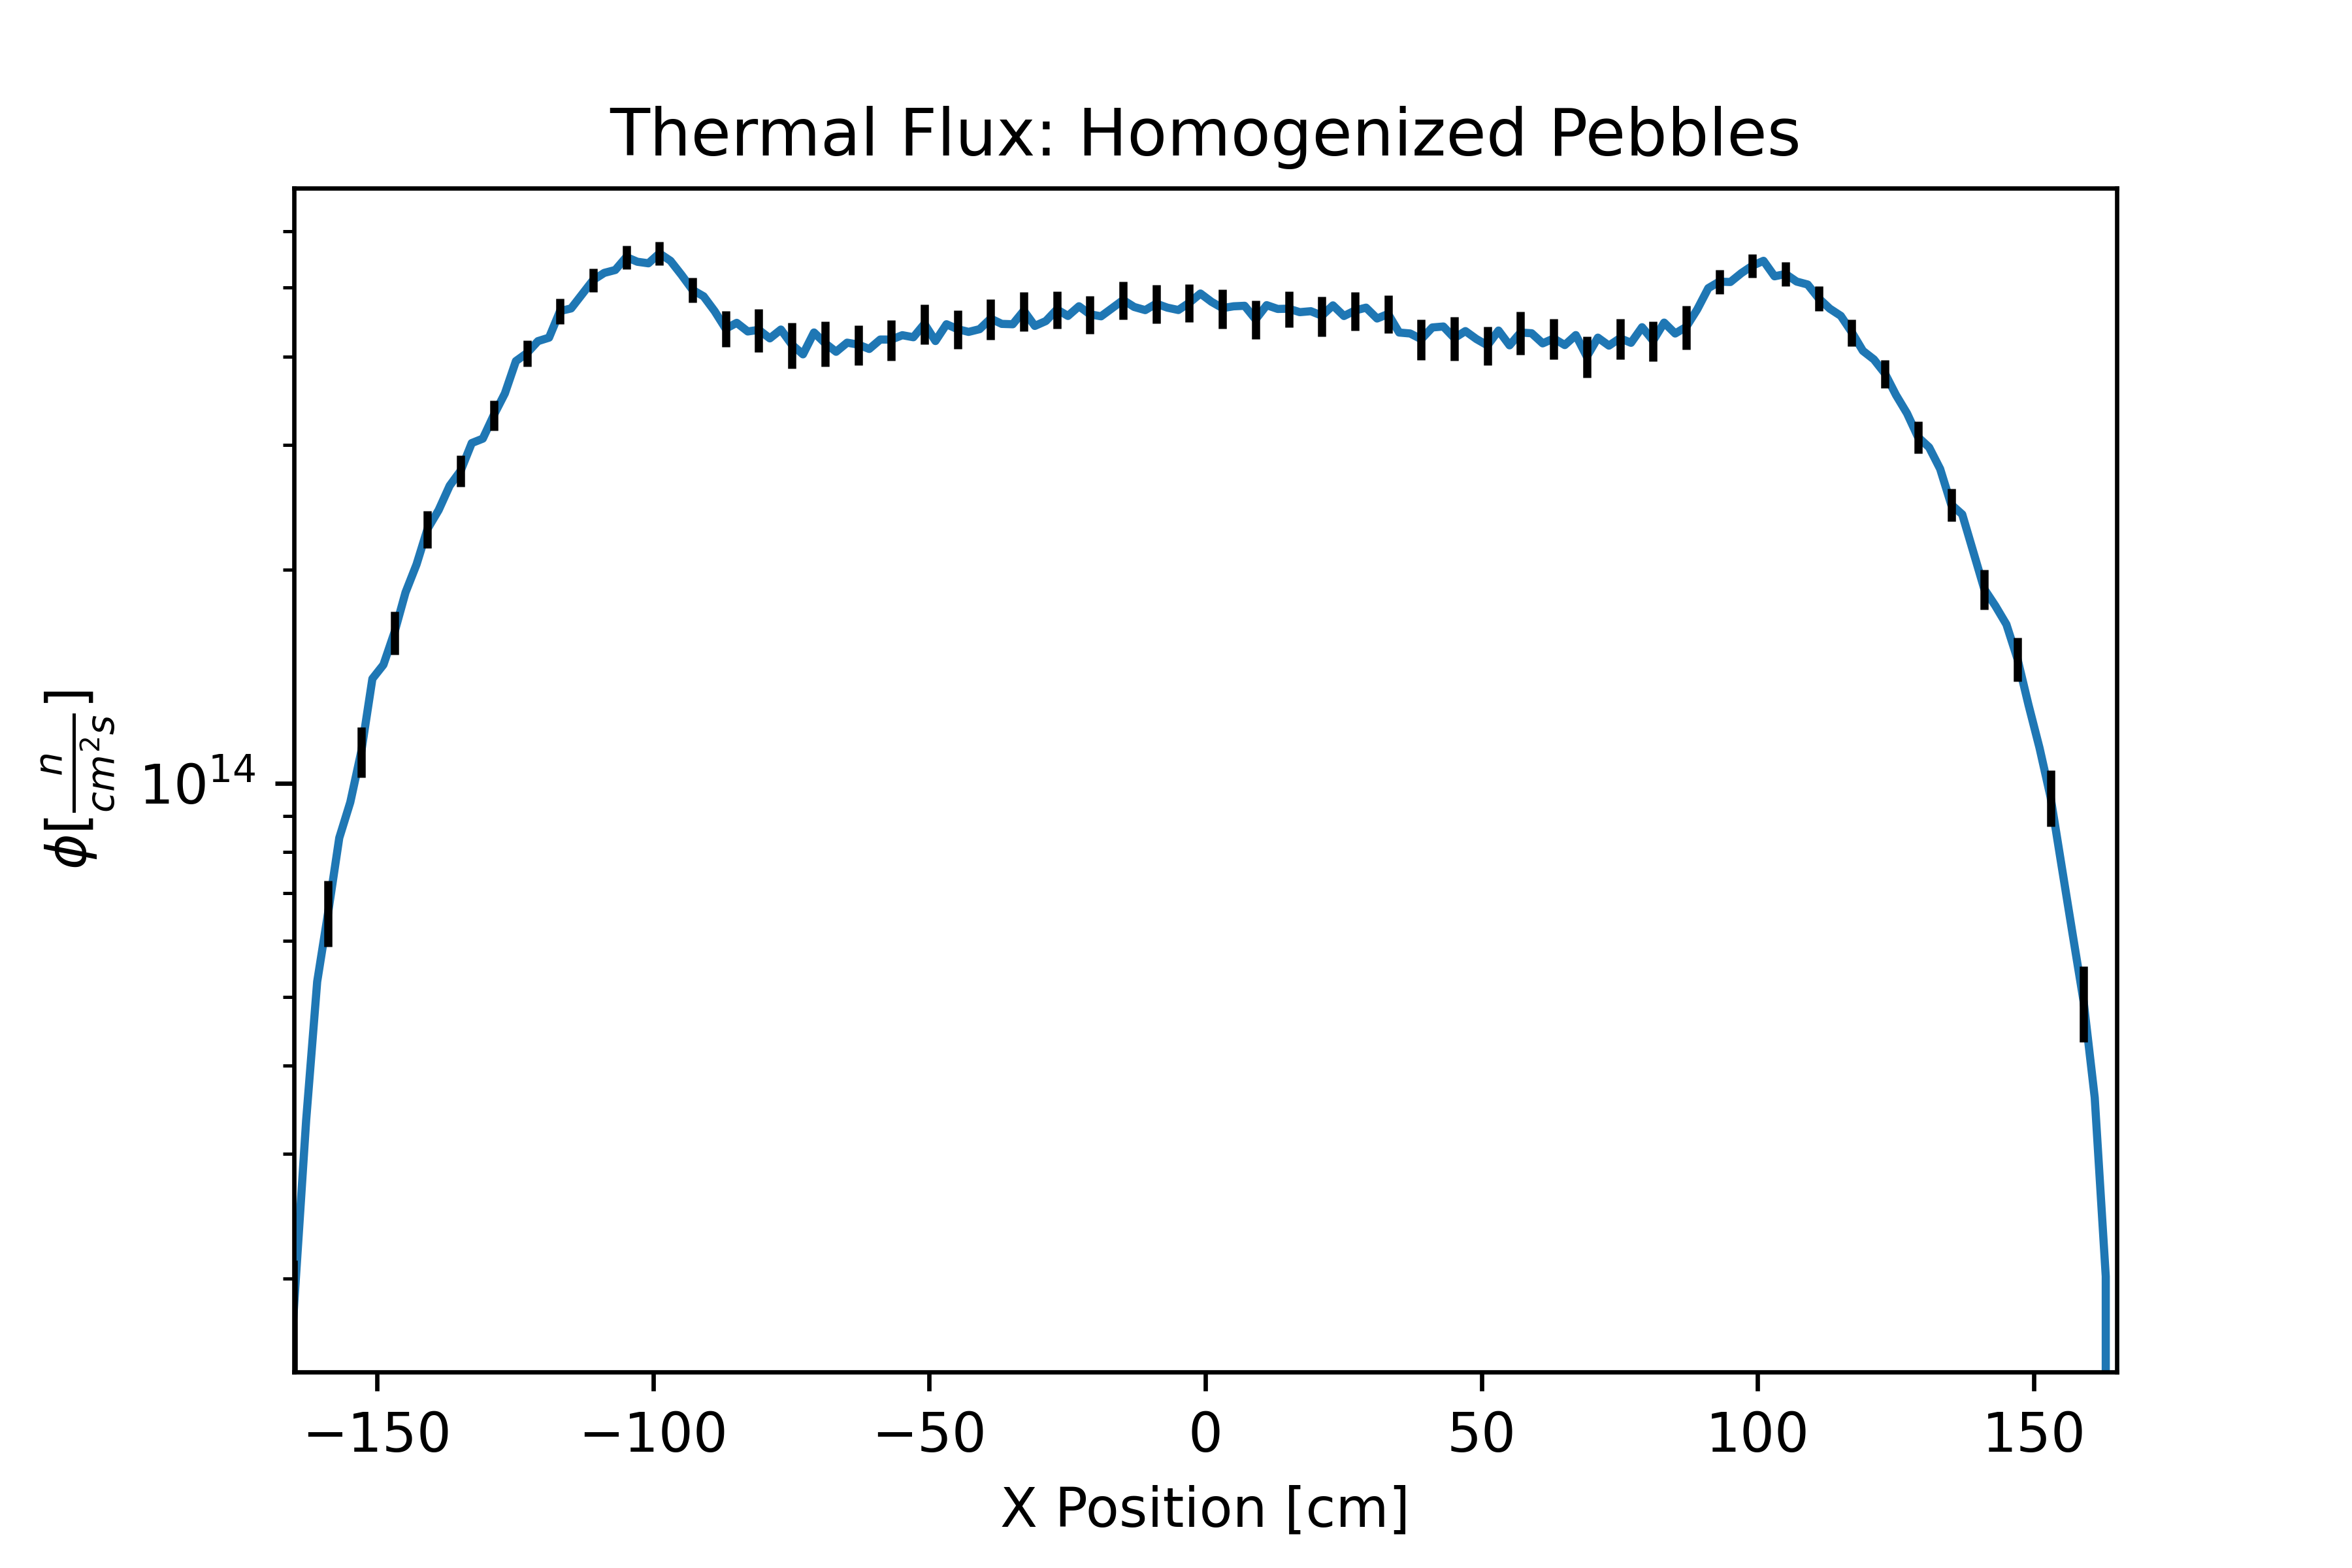
\includegraphics[width=0.95\linewidth]{figures/therm_flux_homog.png}
  \caption{Thermal Flux}
  \label{fig:hom-det-xy-therm}
\end{subfigure}%

\caption{Radial Thermal and Fast Flux Profiles}
\end{figure}

\begin{figure}[H]\ContinuedFloat
\centering

\begin{subfigure}{0.9\textwidth}
  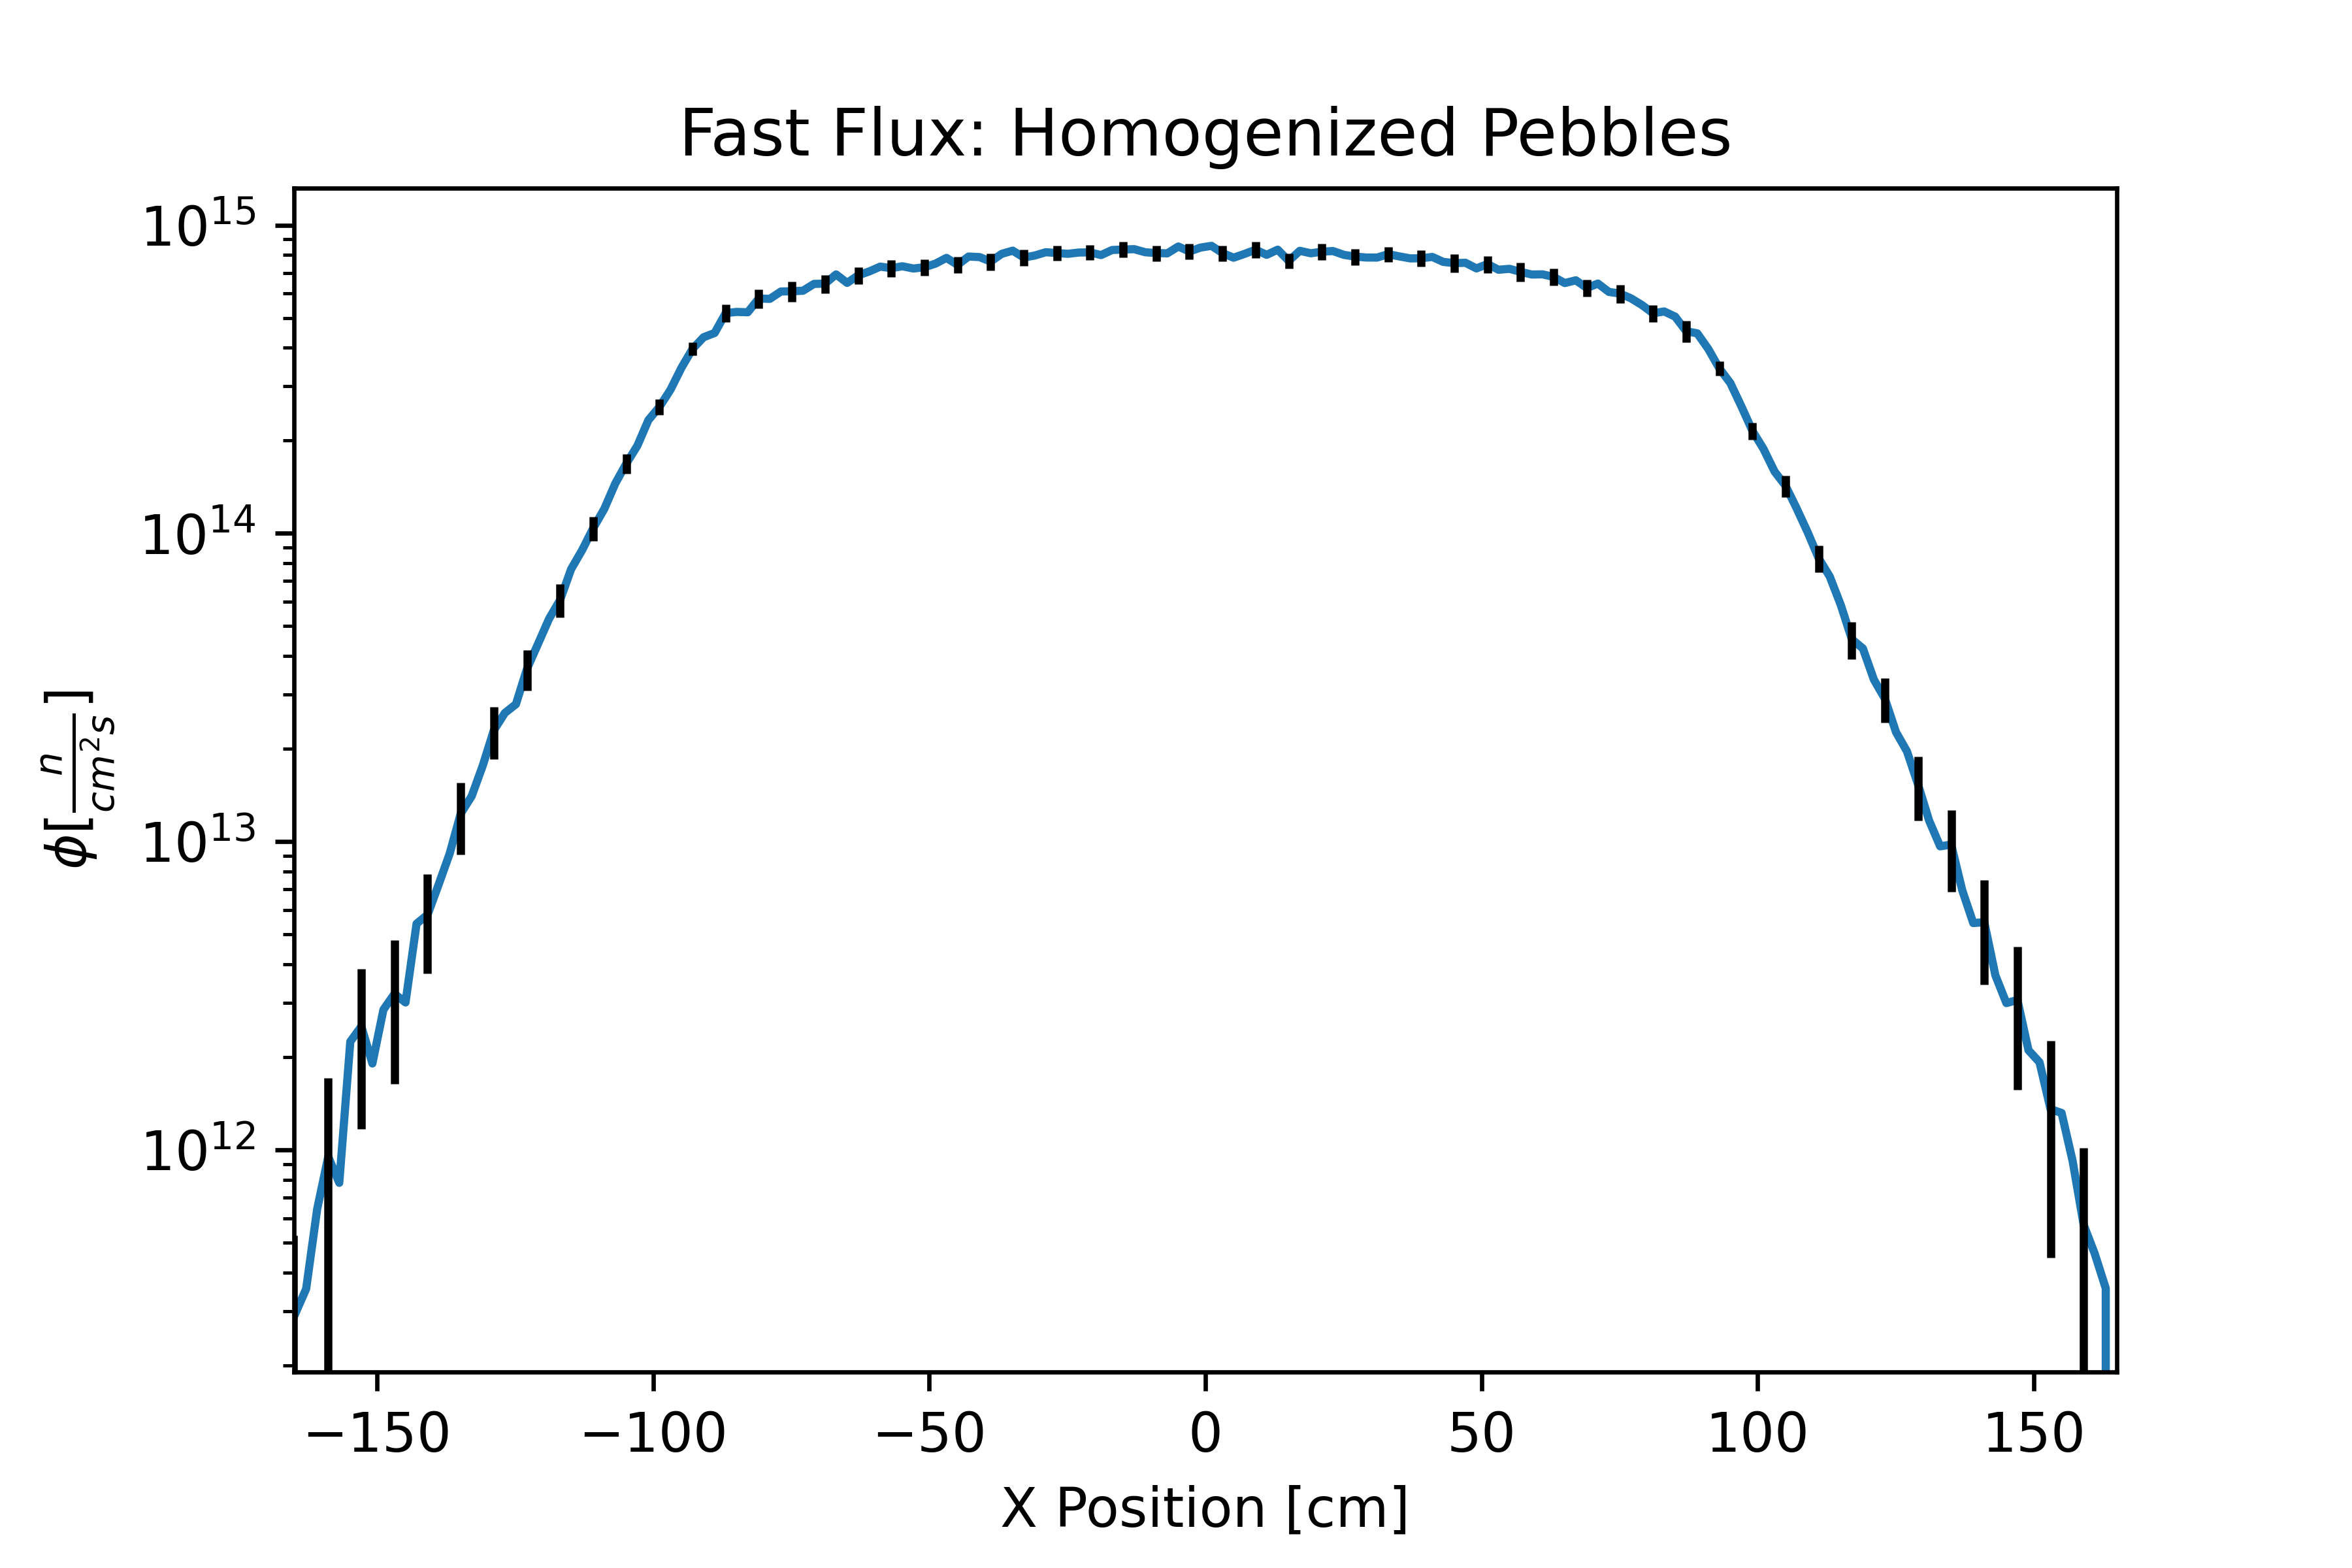
\includegraphics[width=0.95\linewidth]{figures/fast_flux_homog.png}
  \caption{Fast Flux}
  \label{fig:hom-det-xy-fast}
\end{subfigure}

%
\caption{Radial Thermal and Fast Flux Profiles (cont.)}
\label{fig:hom-det-xy}
\end{figure}
\begin{figure}[h!]
\centering

\begin{subfigure}{0.6\textwidth}
  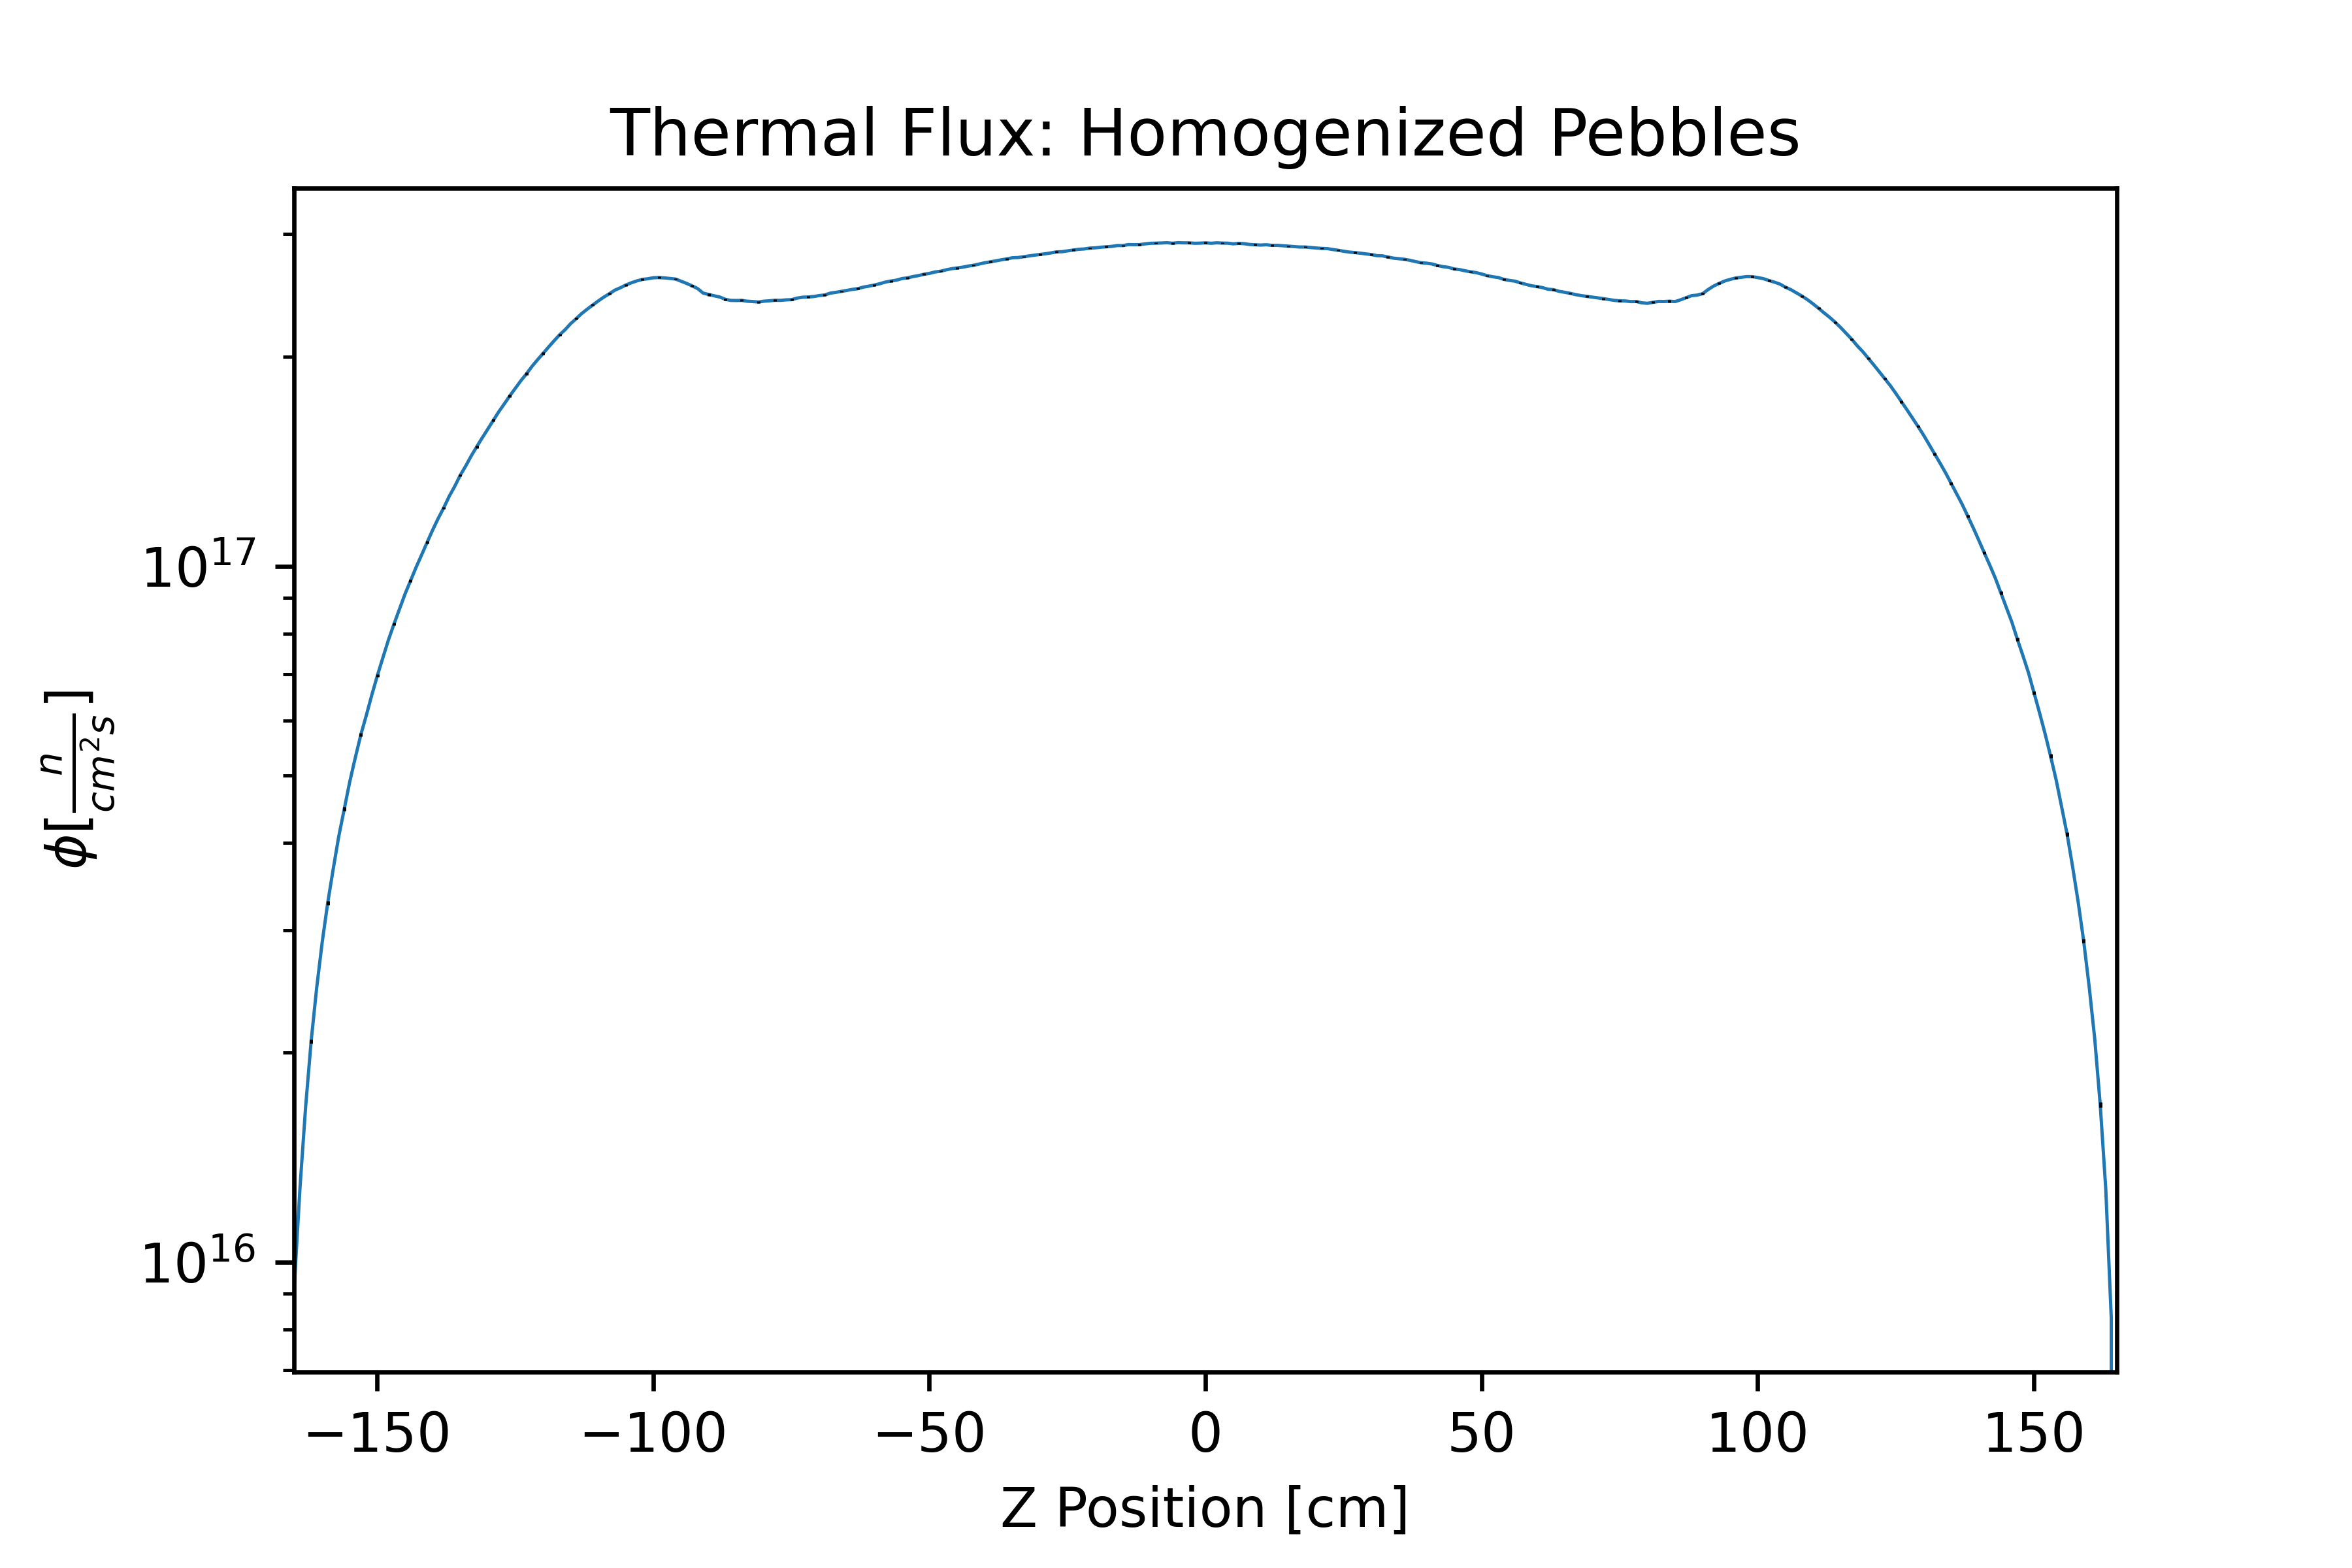
\includegraphics[width=0.95\linewidth]{figures/therm_flux_homog_z.png}
  \caption{Thermal Flux}
  \label{fig:hom-det-z-therm}
\end{subfigure}%
%
\begin{subfigure}{0.6\textwidth}
  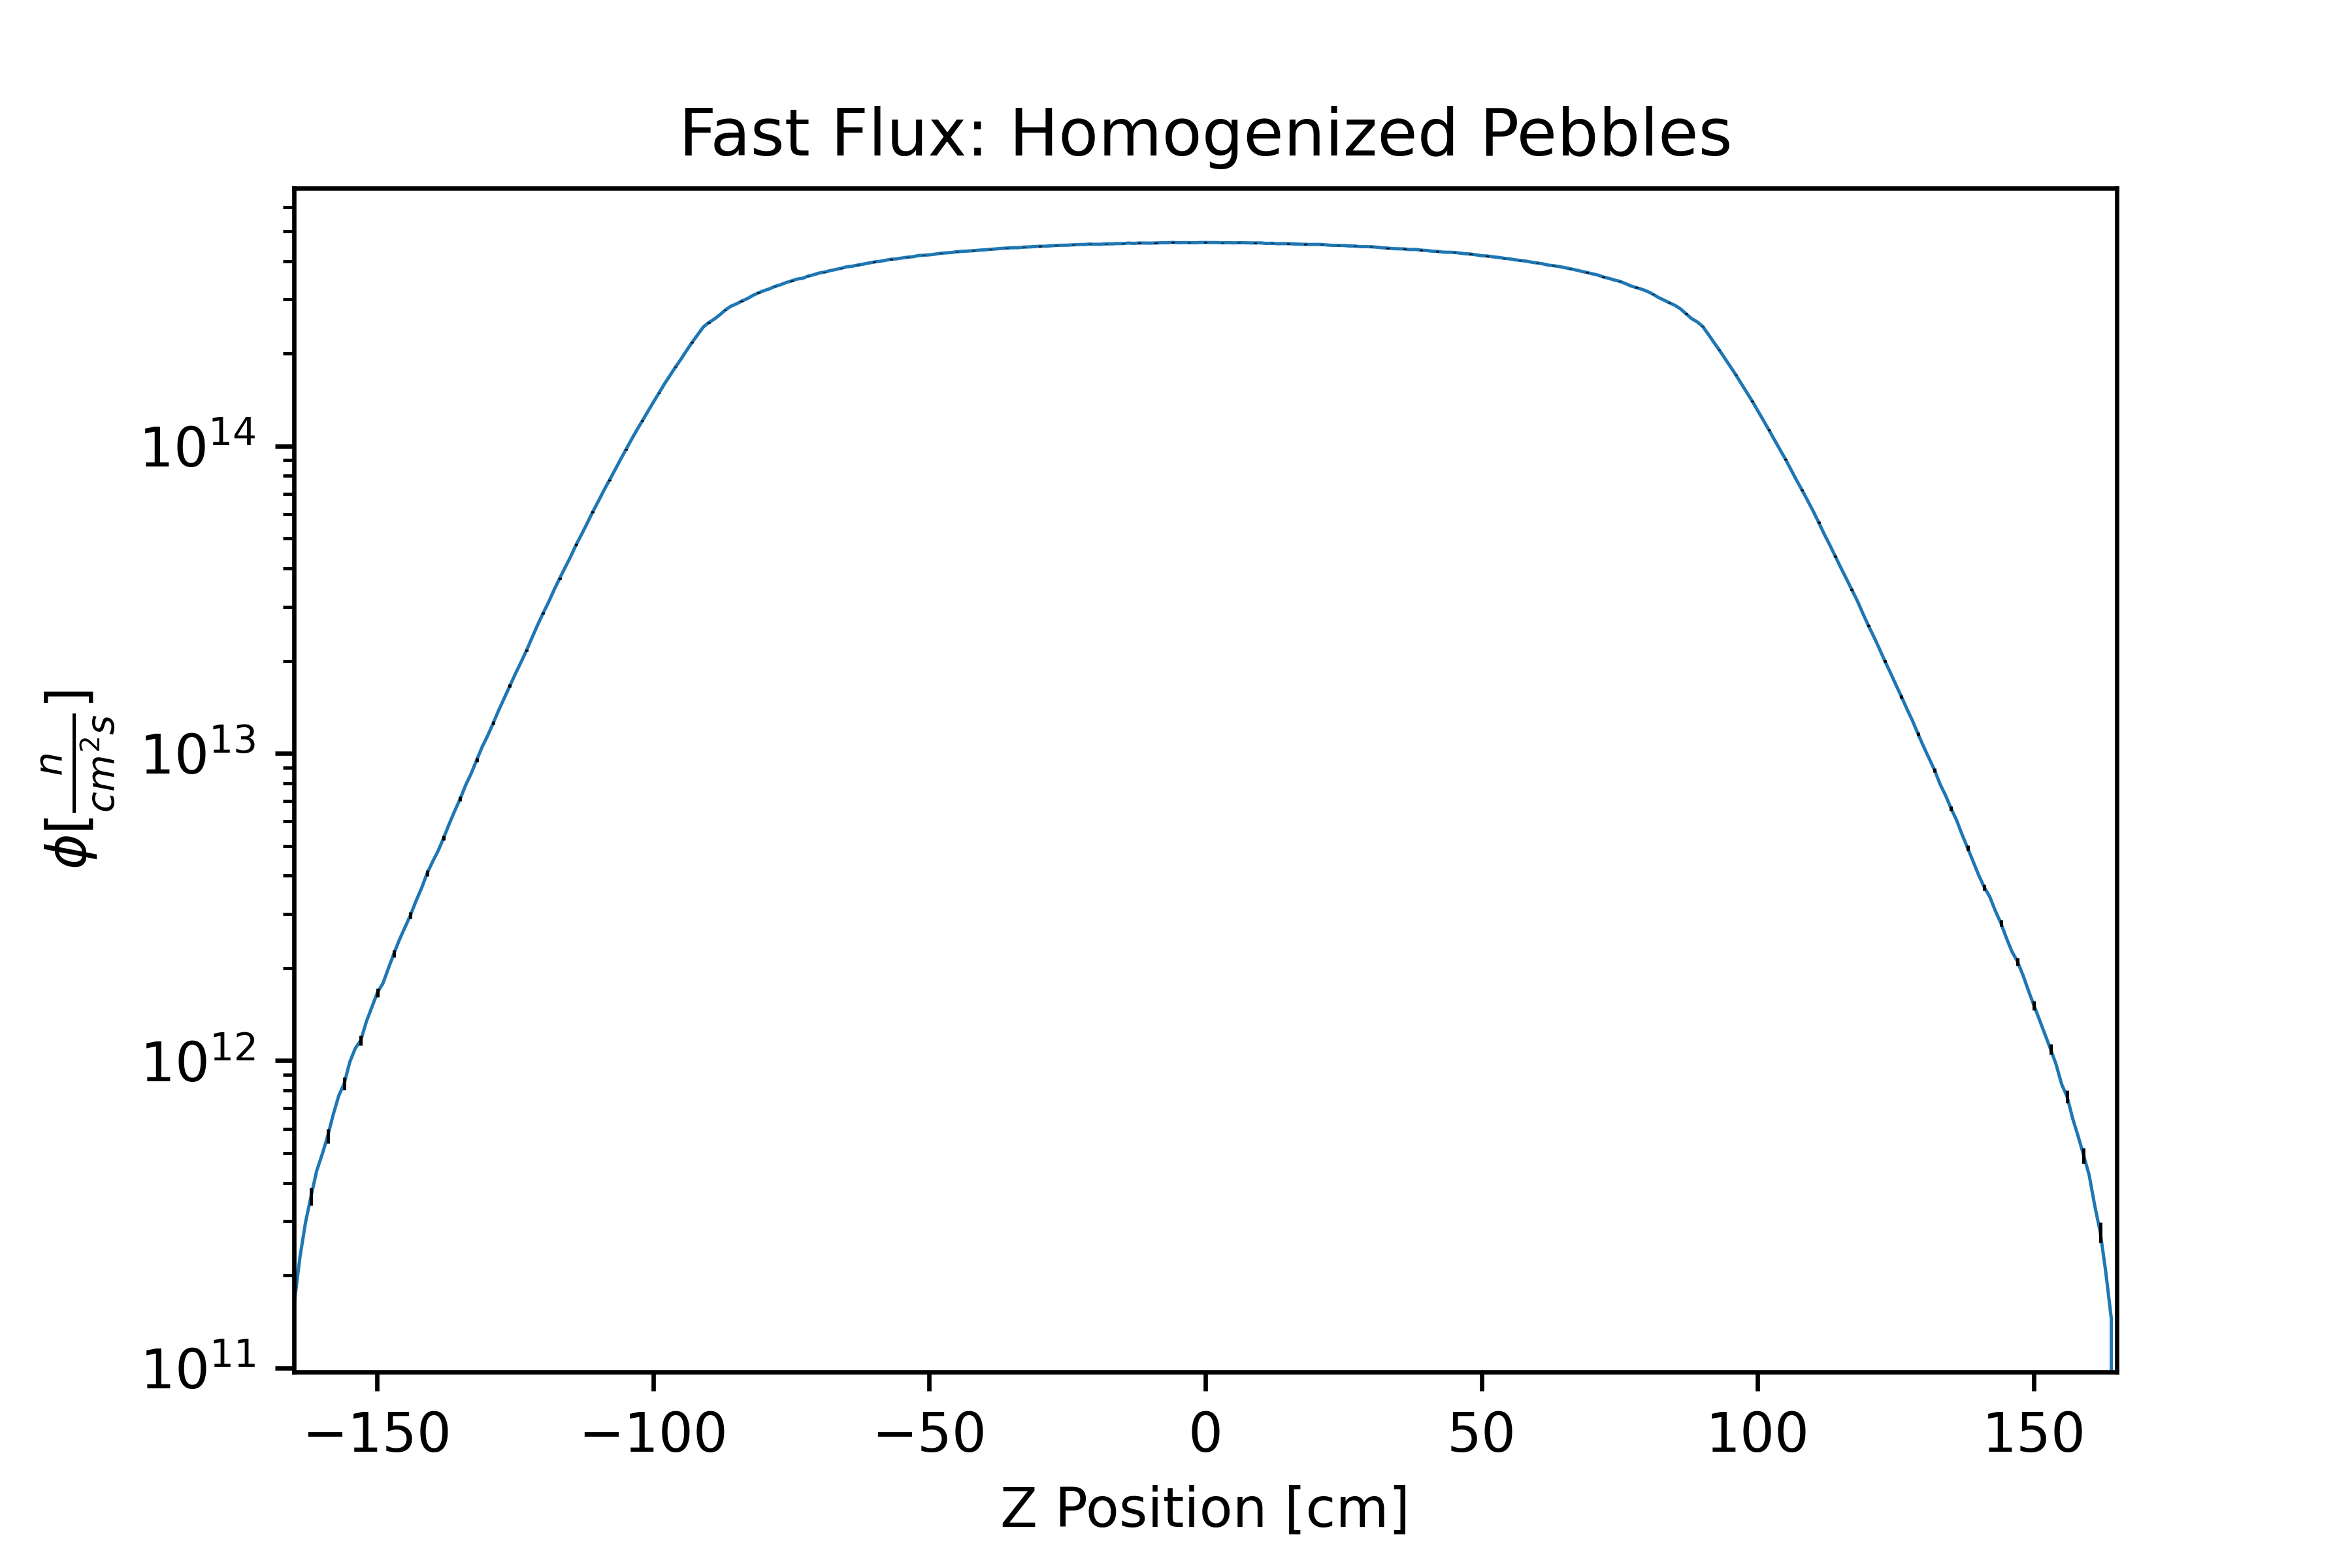
\includegraphics[width=0.95\linewidth]{figures/fast_flux_homog_z.png}
  \caption{Fast Flux}
  \label{fig:hom-det-z-fast}
\end{subfigure}

%
\caption{Axial Thermal and Fast Flux Profiles}
\label{fig:hom-det-z}
\end{figure}

Figures \ref{fig:hom-det-xy} and \ref{fig:hom-det-z} provide the fast and thermal flux profiles in Sangamon20 at the axial and radial (x-direction) centerlines, respectively.  For the radial flux, a detector in the xy plane was used, which had finite bin sizes in x and y, and spanned the whole height of the reactor in the z direction.  For the axial fluxes, the bins were finite in z and spanned the entire diameter of the core.  Normally, these two figures would be subject to the same unequal bin sizing that affected Figure \ref{fig:controlmain}.  To counteract this, the axial fluxes (Figure \ref{fig:hom-det-z}) are multplied by the ratio of the radial detector bin volume to the axial detector bin volume, as follows:

\begin{align}
\phi_{axial, adjusted} &= \phi_{axial, unadjusted}\frac{V_{radial}}{V_{axial}}
\intertext{where}
\phi_{axial, adjusted}&= \mbox{ detector bin-size adjusted flux $\left[\frac{\#}{cm^2s}\right]$}\nonumber\\
\phi_{axial,unadjusted}&= \mbox{ unadjusted axial flux $\left[\frac{\#}{s}\right]$}\nonumber\\
V_{radial}&=\mbox{ radial detector bin volume $[cm^3]$}\nonumber\\
V_{axial}&=\mbox{ axial detector bin volume $[cm^3]$}\nonumber
\end{align}

Both axially and radially, the thermal flux sees a 'bump', which peaks approximately 10 cm into the reflector, at 100 cm.  These are the highest peaks in the thermal flux, with the second highest thermal flux being at the center line.  For the fast flux profile we see a flattened peak in the  active core (-90.0 cm to 90 cm).  Fast flux rapidly decreases in the reflector as fast neutrons down scatter in the graphite.  Both Figures \ref{fig:hom-det-xy} and \ref{fig:hom-det-z} show that while the radial banding seen in the fission rate mesh profiles are of high intensity, the flux peaks are elsewhere.

In addition to centerline fast and thermal flux profiles, Figures \ref{fig:hom-plane-fast} and \ref{fig:hom-plane-therm} provide the fast and thermal flux profiles in the xy plane.

\begin{figure}[H]
\centering

  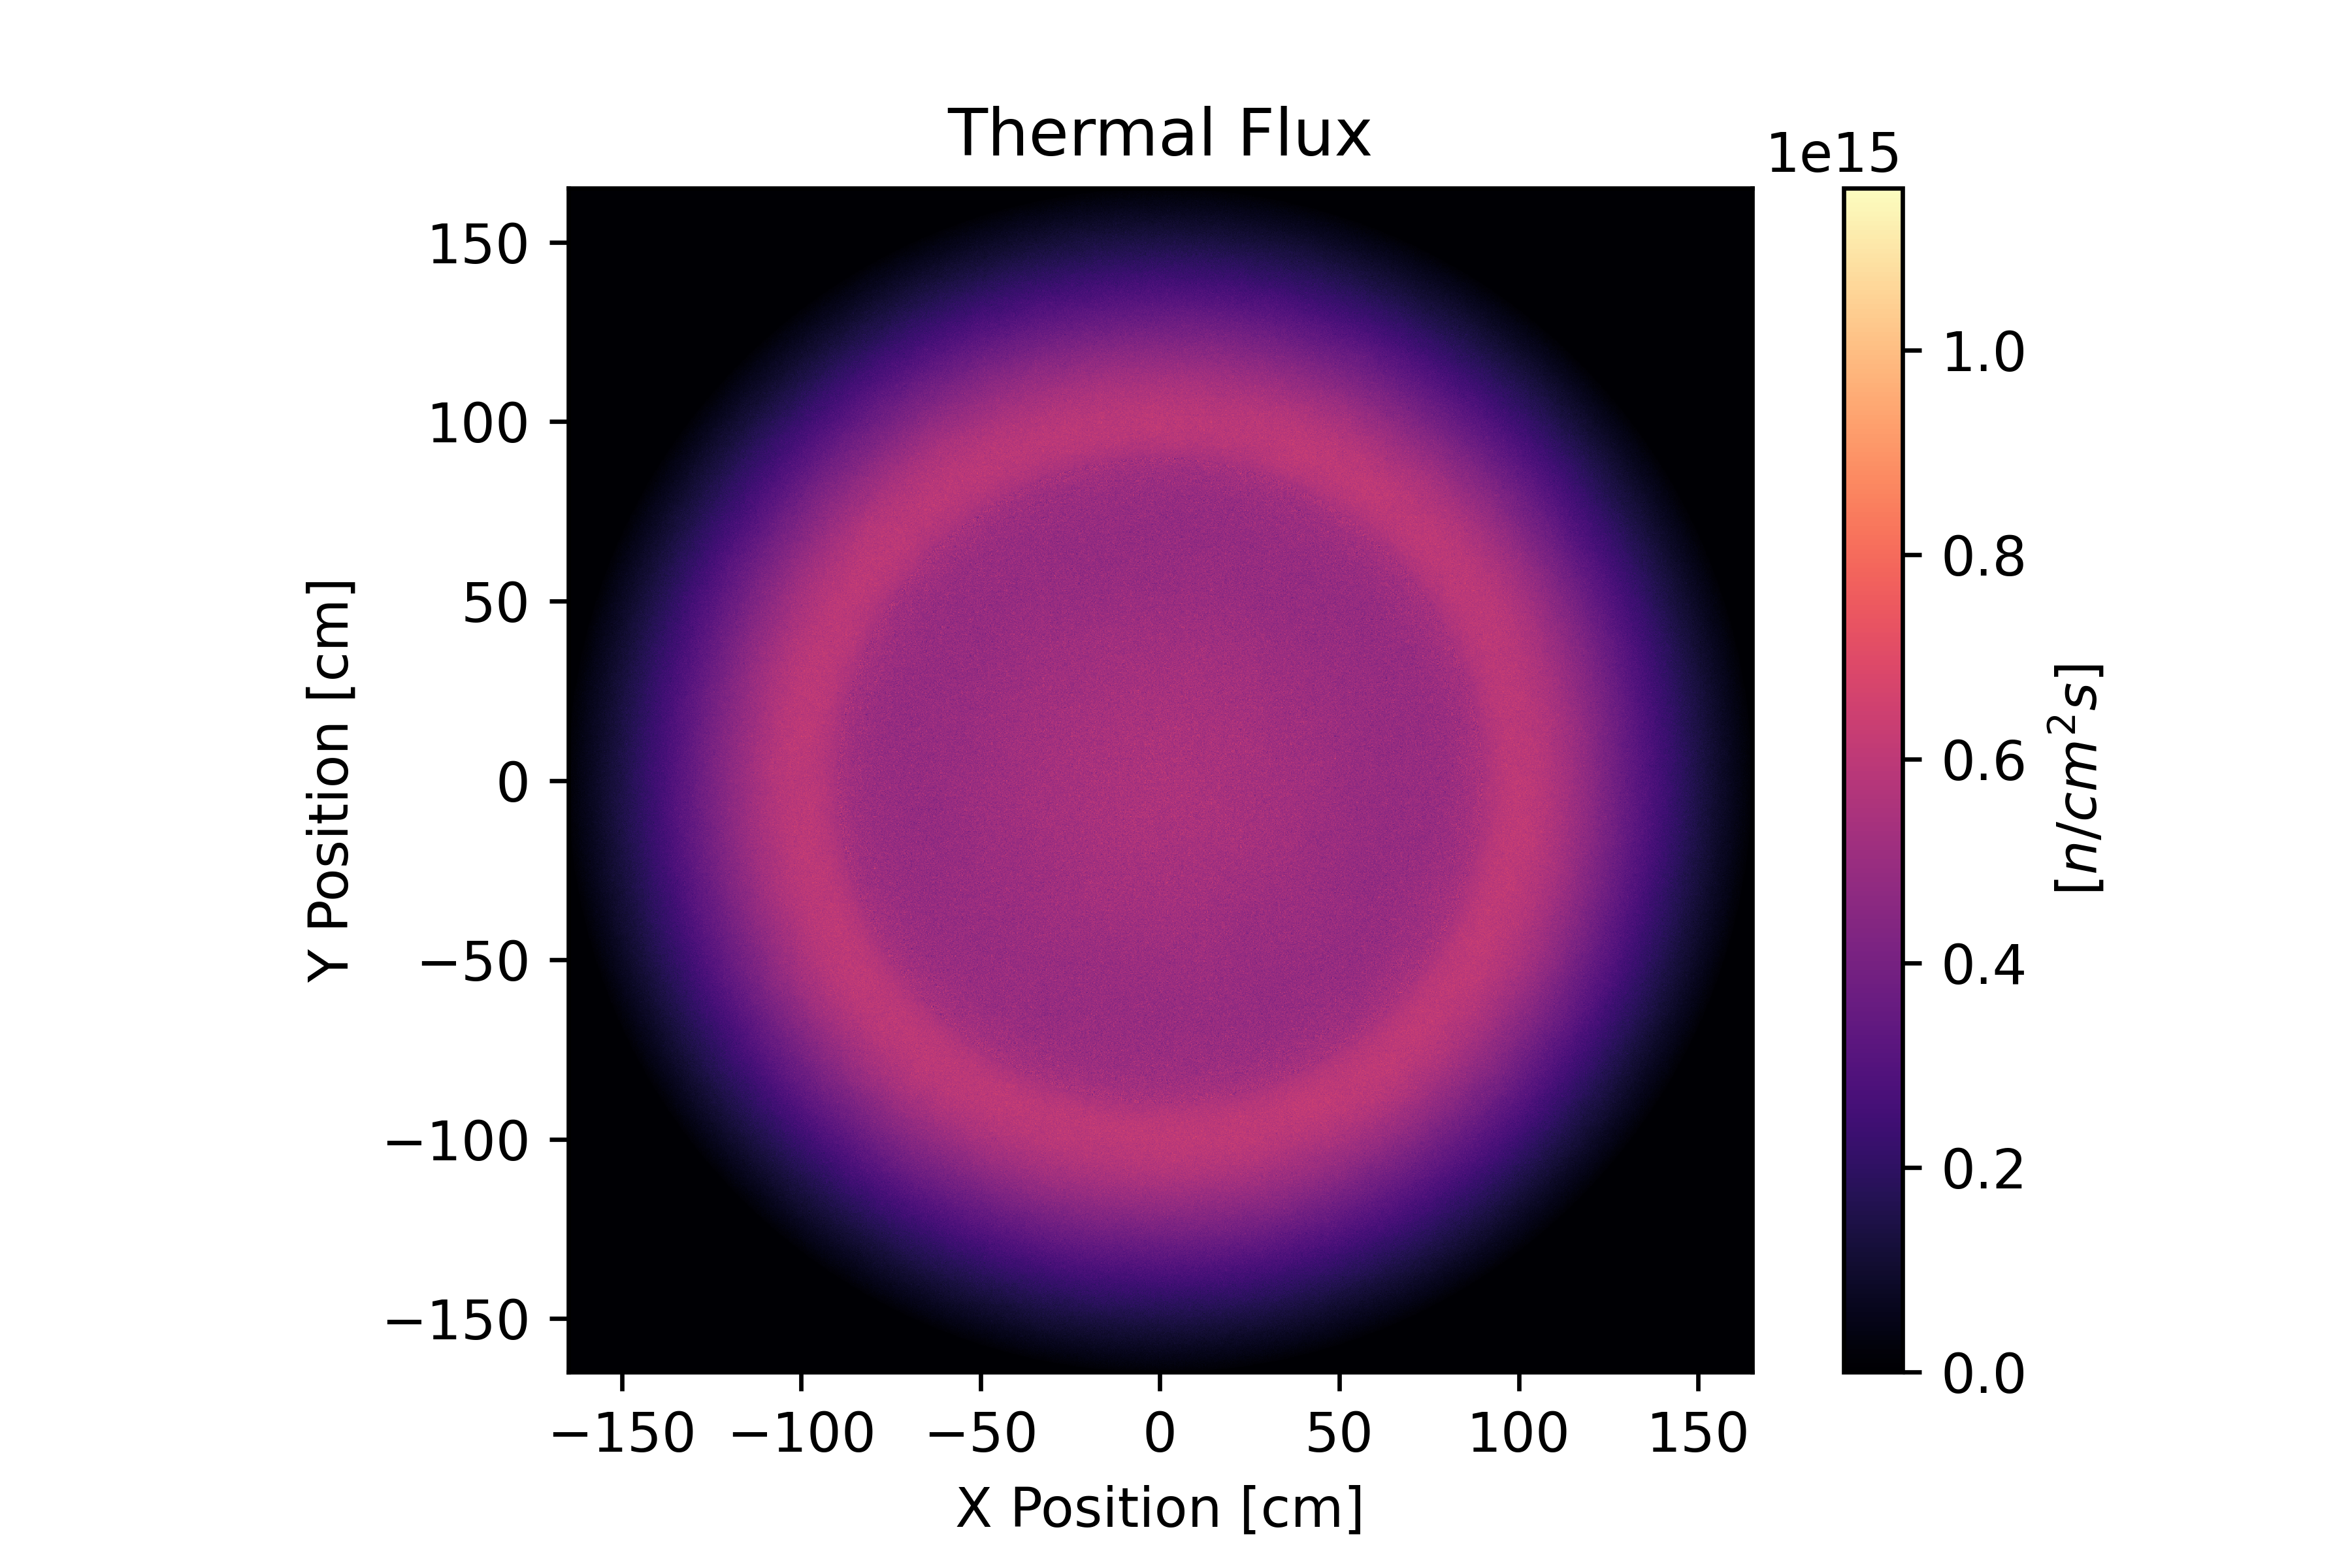
\includegraphics[width=1.0\linewidth]{figures/therm_xy_plane_homog_er.png}
  \caption{Thermal Flux in xy Plane in Sangamon20: Homogenized Pebbles.  The dotted line annotation marks the boundary between the active core and the graphite reflector.}
  \label{fig:hom-plane-therm}

\end{figure}


\begin{figure}[H]
\centering

 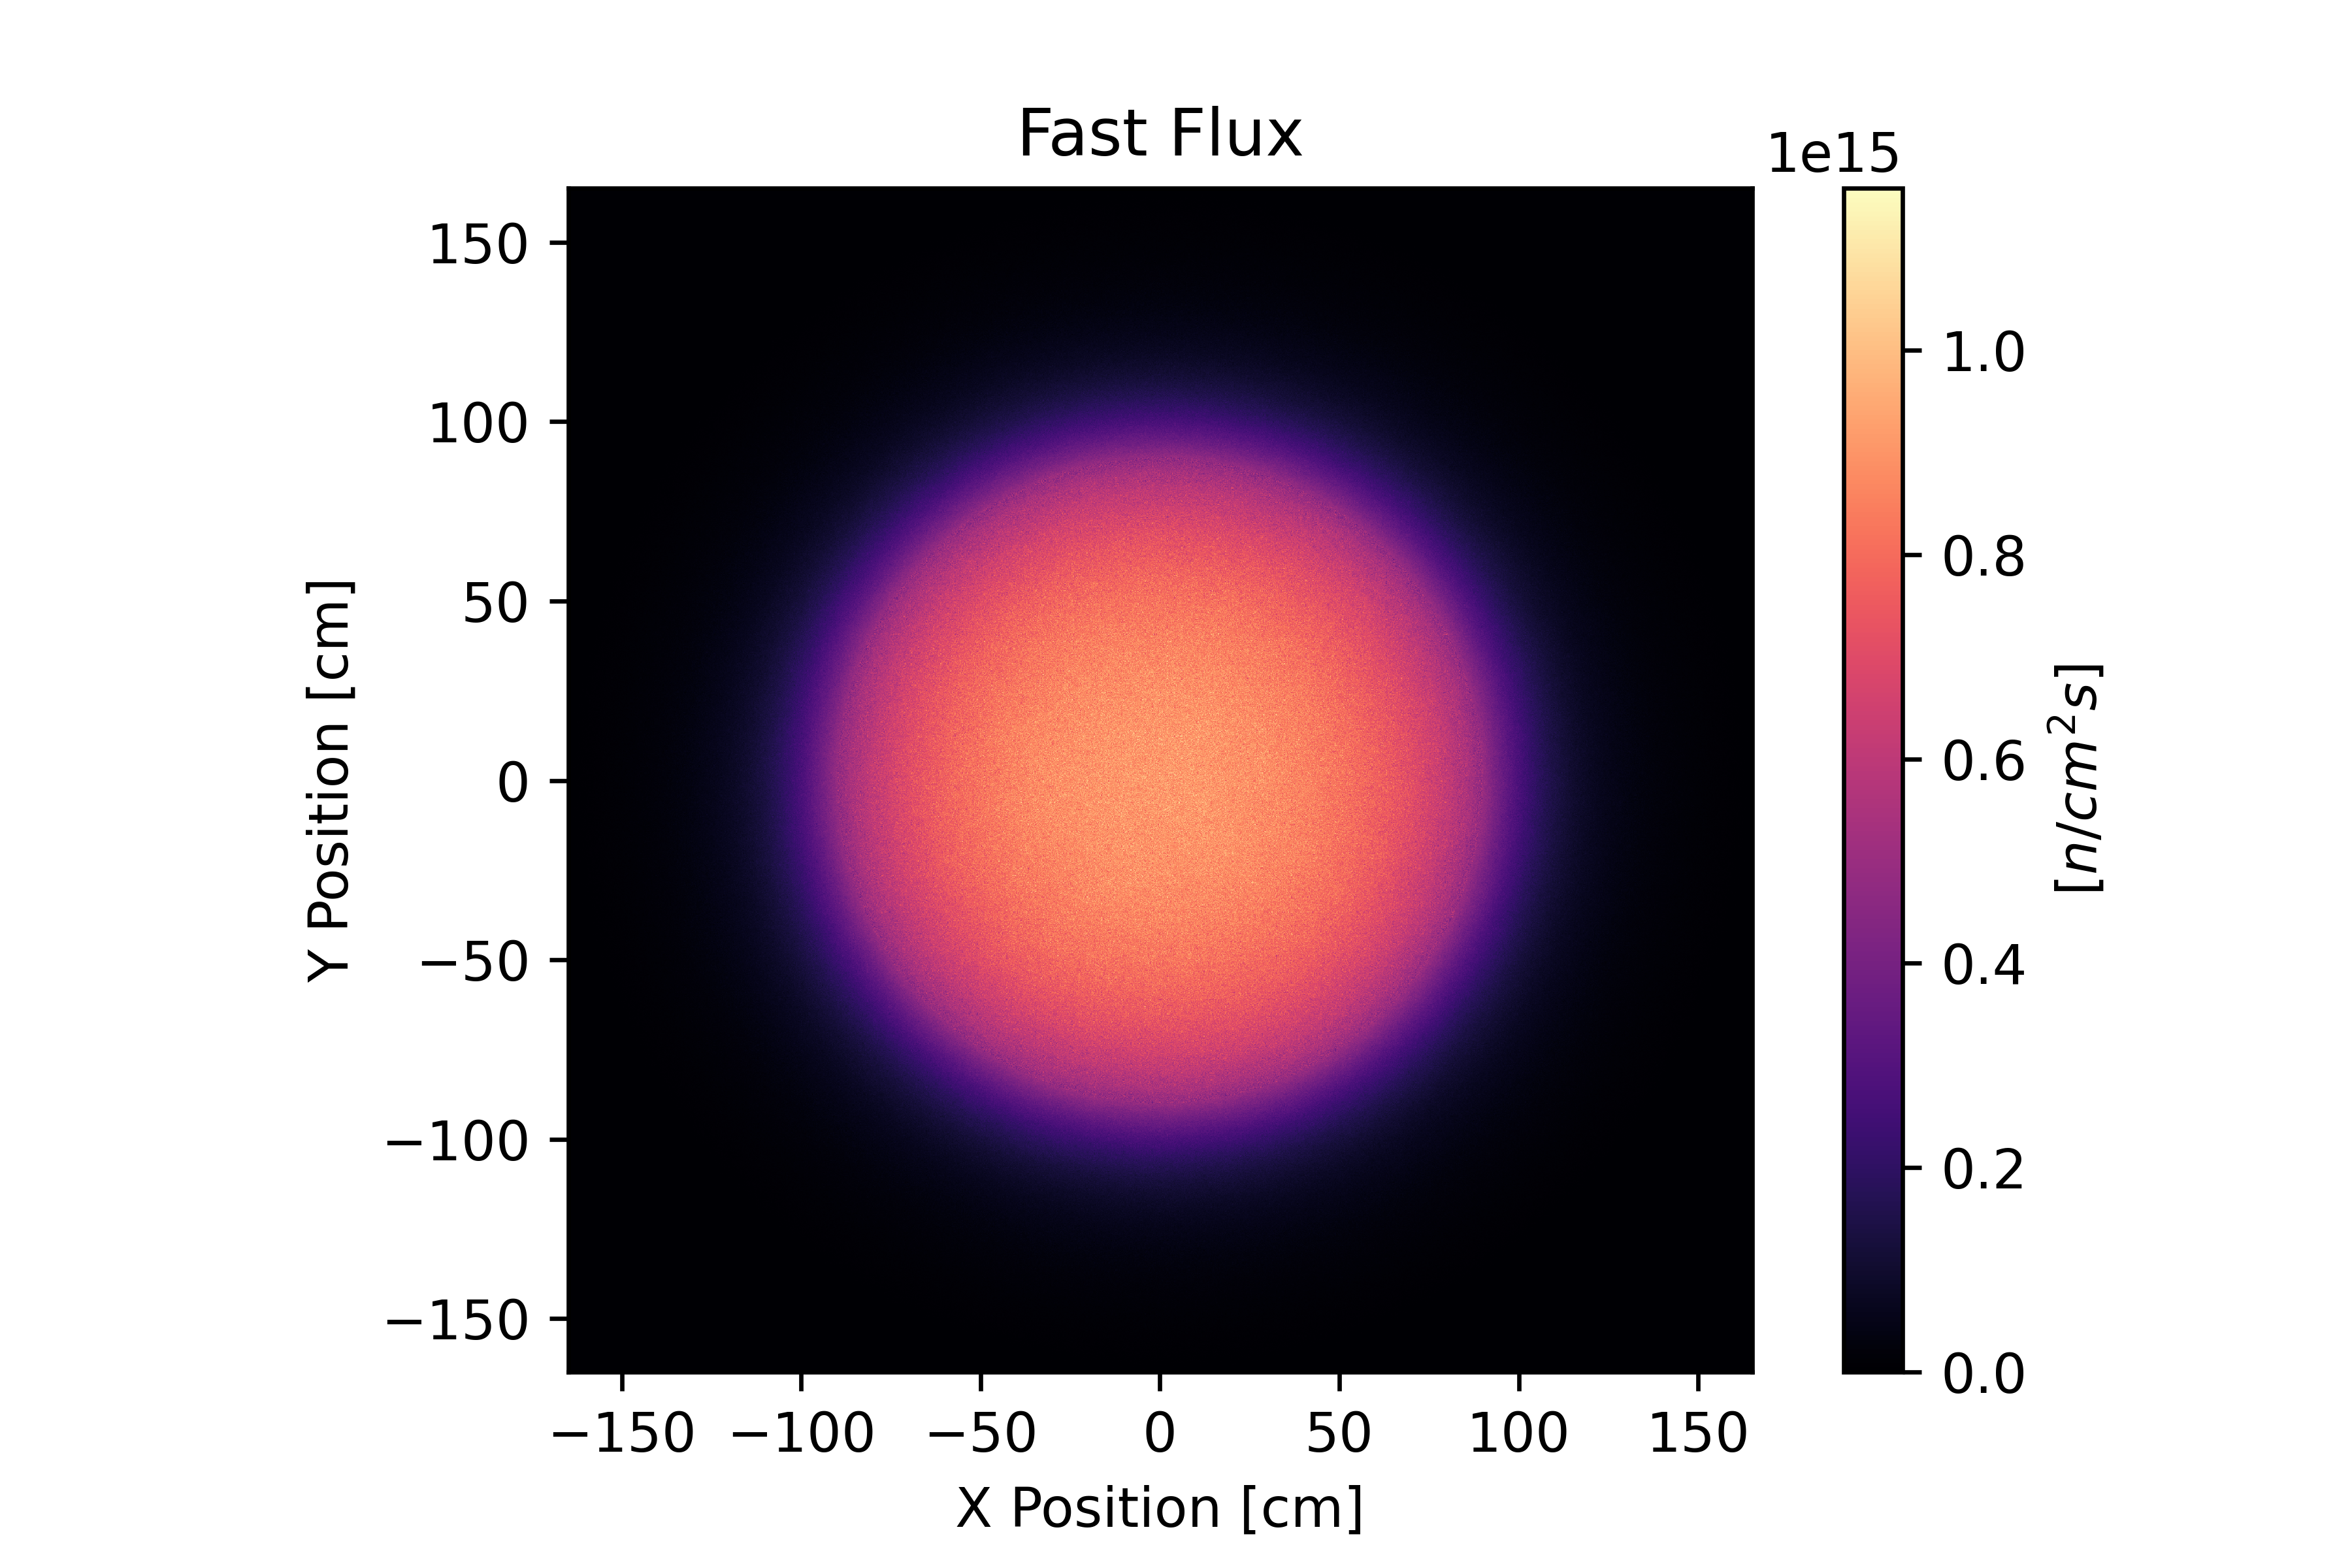
\includegraphics[width=1.0\linewidth]{figures/fast_xy_plane_homog_er.png}
 \caption{Fast Flux in xy Plane in Sangamon20: Homogenized Pebbles.  The dotted line annotation marks the boundary between the active core and the graphite reflector.}
 \label{fig:hom-plane-fast}

\end{figure}

A slight banding pattern on the active core's edge exists --- primarily in the fast, rather than thermal, flux --- but with less intensity than the fission rate banding.  In the thermal flux, we see that the peak in \ref{fig:hom-det-xy} continues in a circular pattern surrounding the active core, approximately 10 cm into the graphite reflector.  The steep drop-off in fast flux once within the outer reflector, meanwhile, is clearer in \ref{fig:hom-plane-fast}.  Once again, Figure \ref{fig:hom-plane-fast} and Figure \ref{fig:hom-plane-therm} show that while the banding morphology may be present in the fission rate profile (and do cause a slight increase relative to the region immediately surrounding it) it does not cause concentric spikes in the flux profiles.  It is suspected that the banding pattern is less prevalent in the thermal flux because the banded region is directly next to the reflector, which has a smoothing effect.

Figures \ref{fig:hom-core} through \ref{fig:hom-cool} gives the energy spectra in the reflector, coolant, overall core, and a randomly selected fresh and sixth-pass pebble.  The results are per unit lethargy and use the Tripoli 315-group energy structure \cite{noauthor_tripoli_nodate} to set energy bin boundaries.  This group structure was chosen not only because there were a sufficient number of bins to provide the desired fidelity, but also because the highest fidelity regions (smallest bin size) in the spectrum were in the lower energy values, which is of greater interest to a thermal spectrum reactor.

\begin{figure}[H]
\centering
  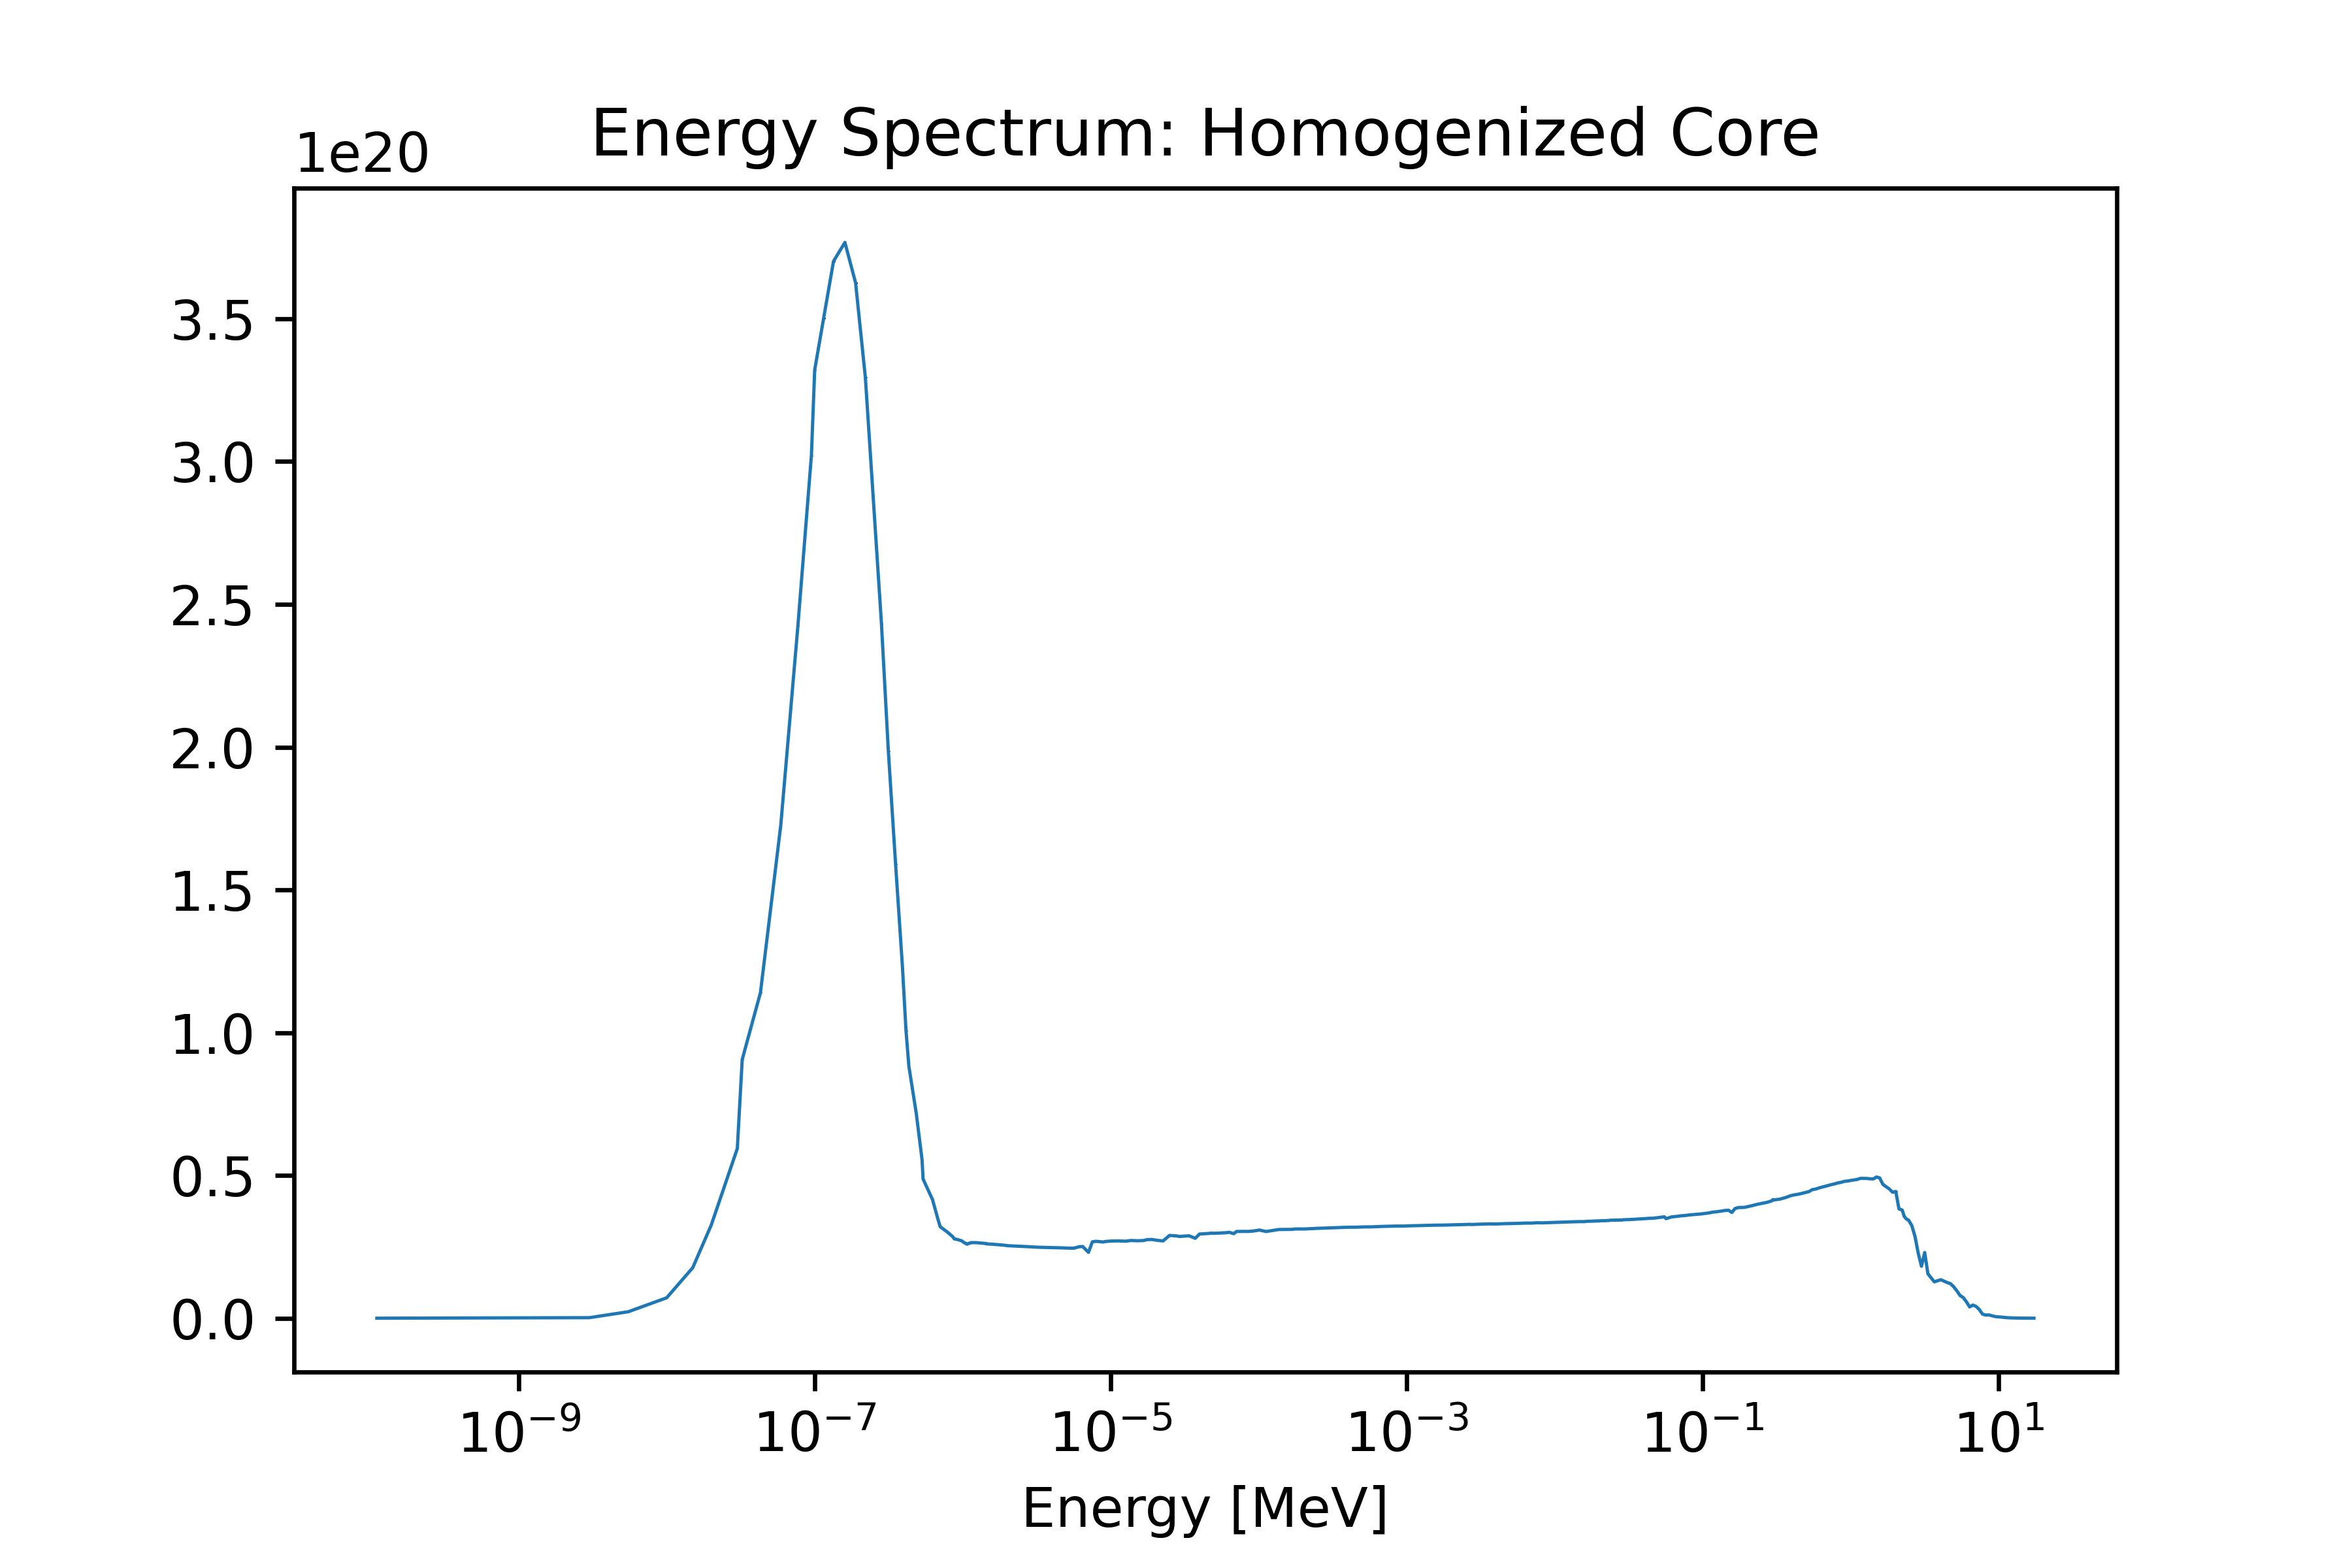
\includegraphics[width=0.95\linewidth]{figures/core_spec_homog}
  \caption{Lethargy Adjusted Neutron Flux Energy Spectrum in the Whole-Core for the Homogenized-Pebble Sangamon20}
  \label{fig:hom-core}
\end{figure}

\begin{figure}[H]
\centering
  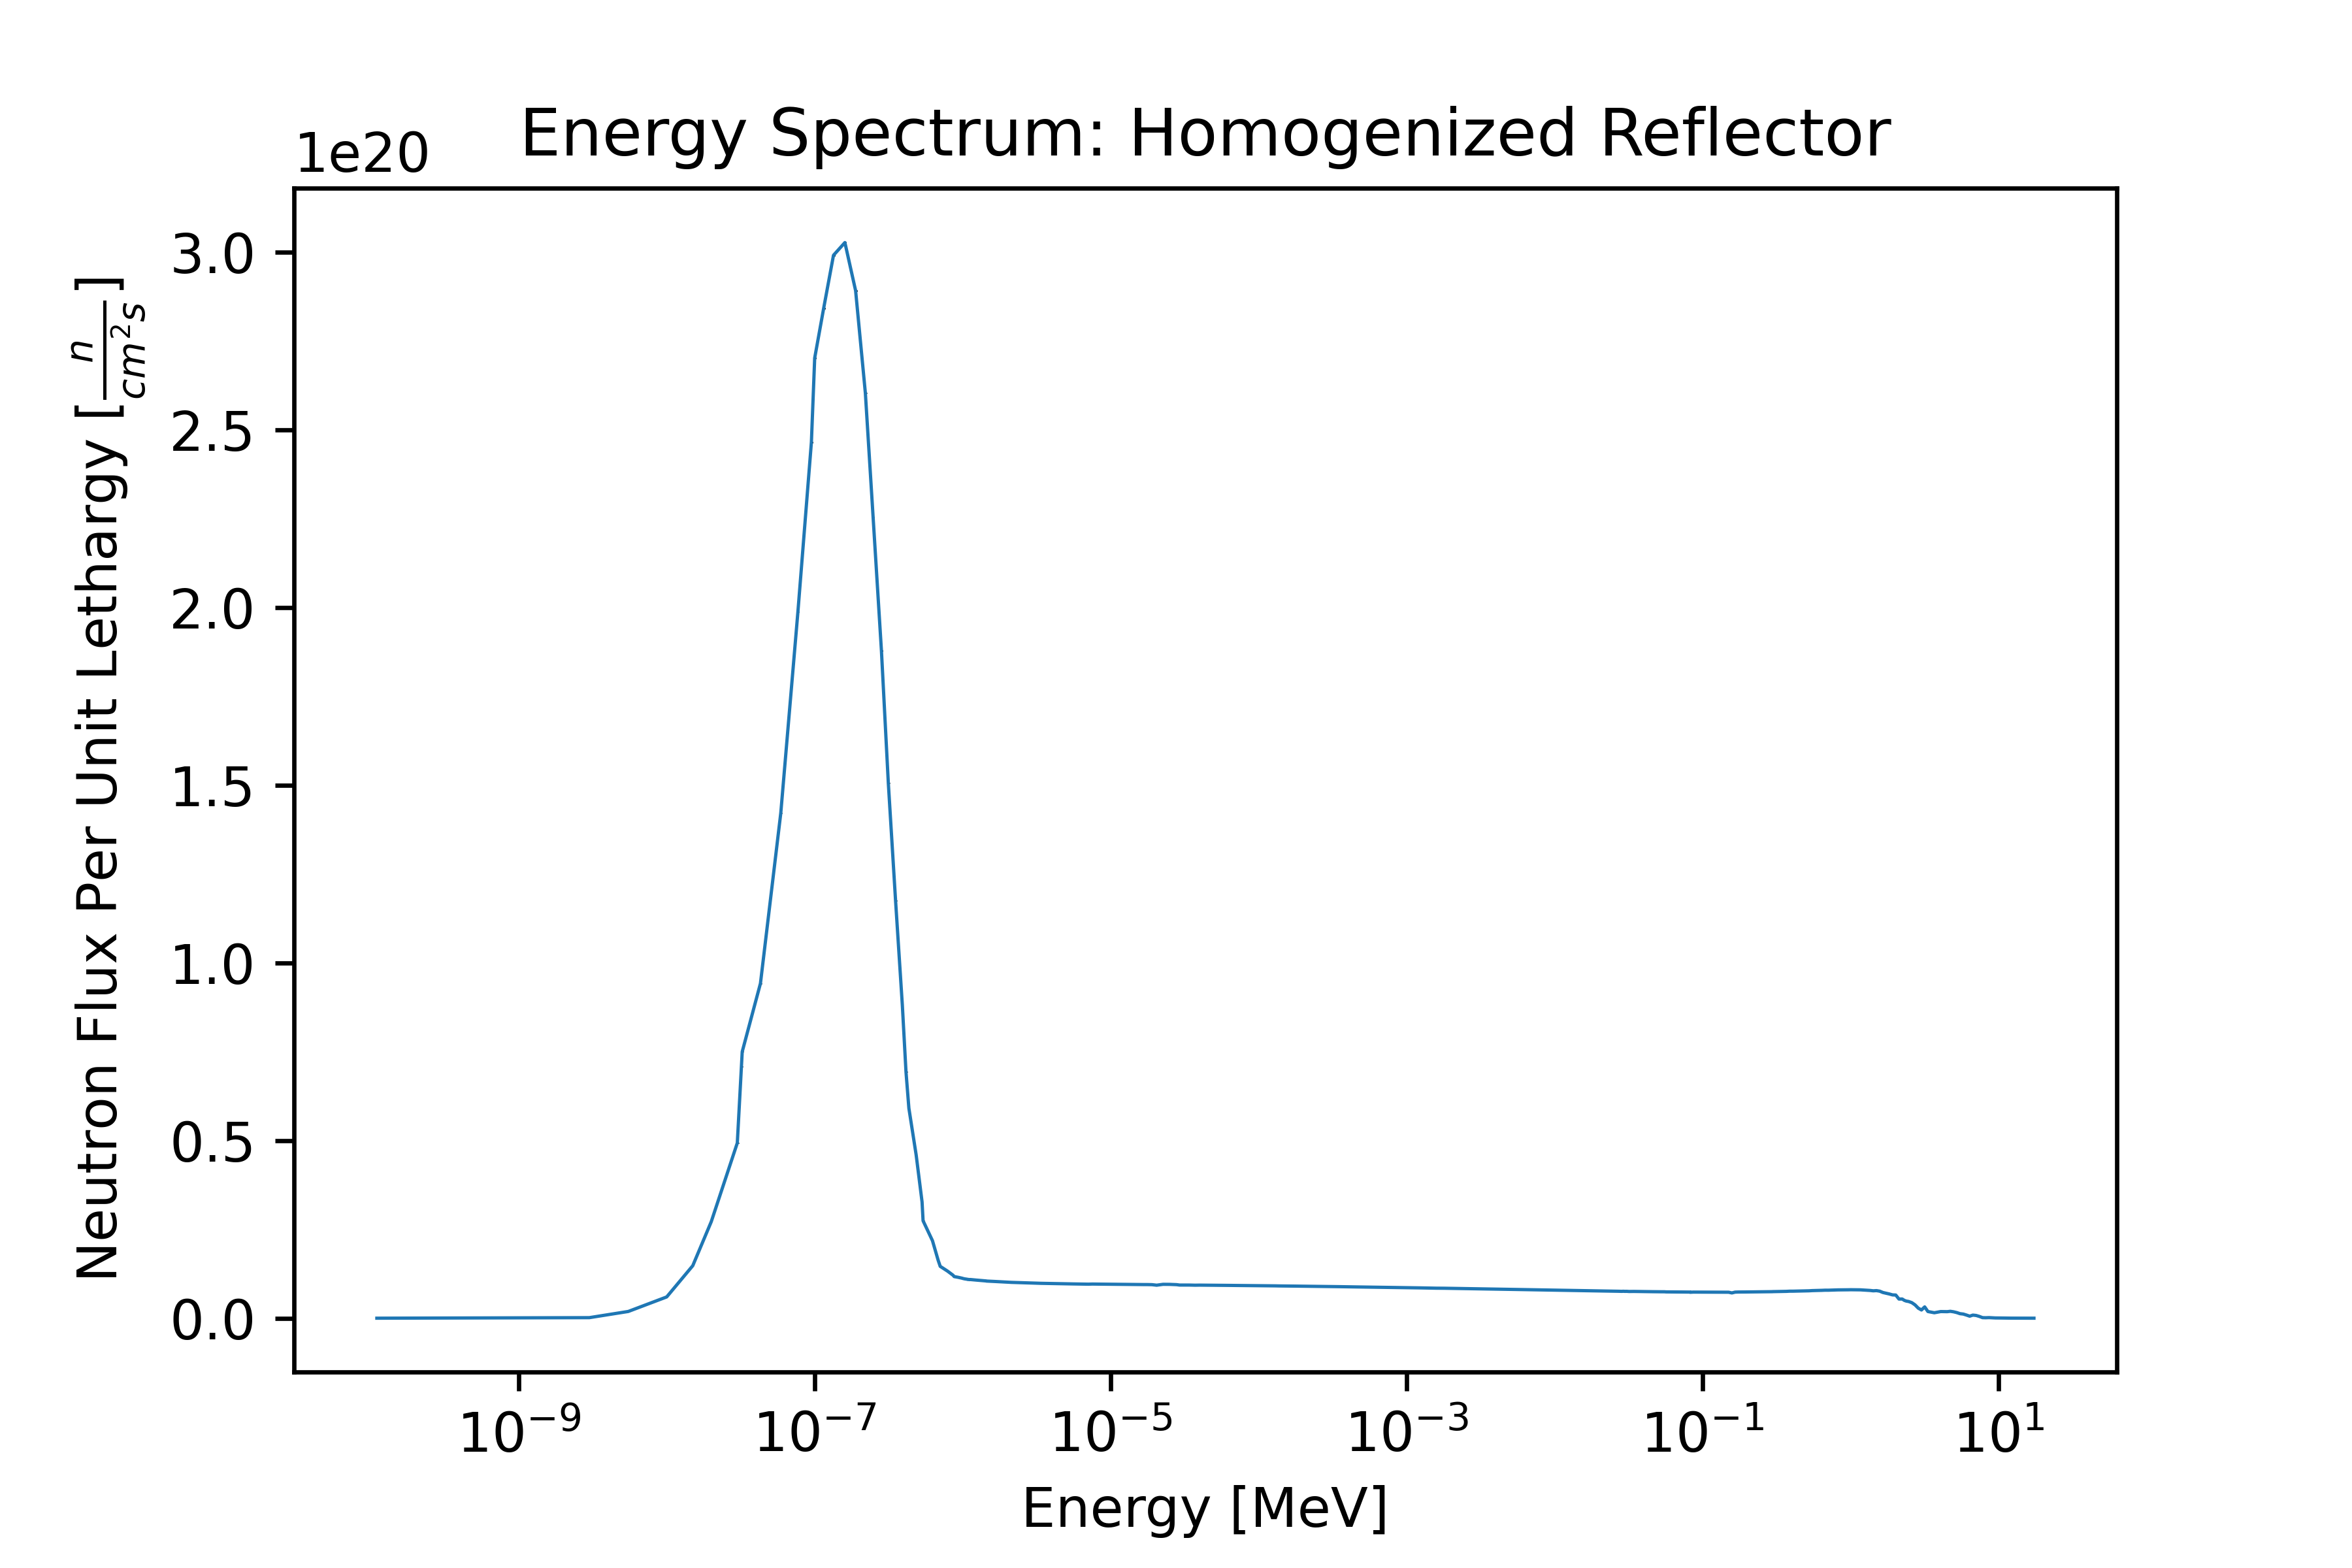
\includegraphics[width=0.95\linewidth]{figures/reflect_spec_homog}
  \caption{Lethargy Adjusted Neutron Flux Energy Spectrum in the Reflector for the Homogenized-Pebble Sangamon20}
  \label{fig:hom-reflec}
\end{figure}


The thermal peak of the whole-core and reflector both occur around $10\times10^{-07}$ MeV, which is also the energy of neutrons most-responsible for fission.  The thermalization of neutrons in the reflector dominates the spectrum in Figure \ref{fig:hom-core}, indicated by the high magnitude of the thermal peak in the reflector and core and their similar shape.


\begin{figure}[H]
\centering
  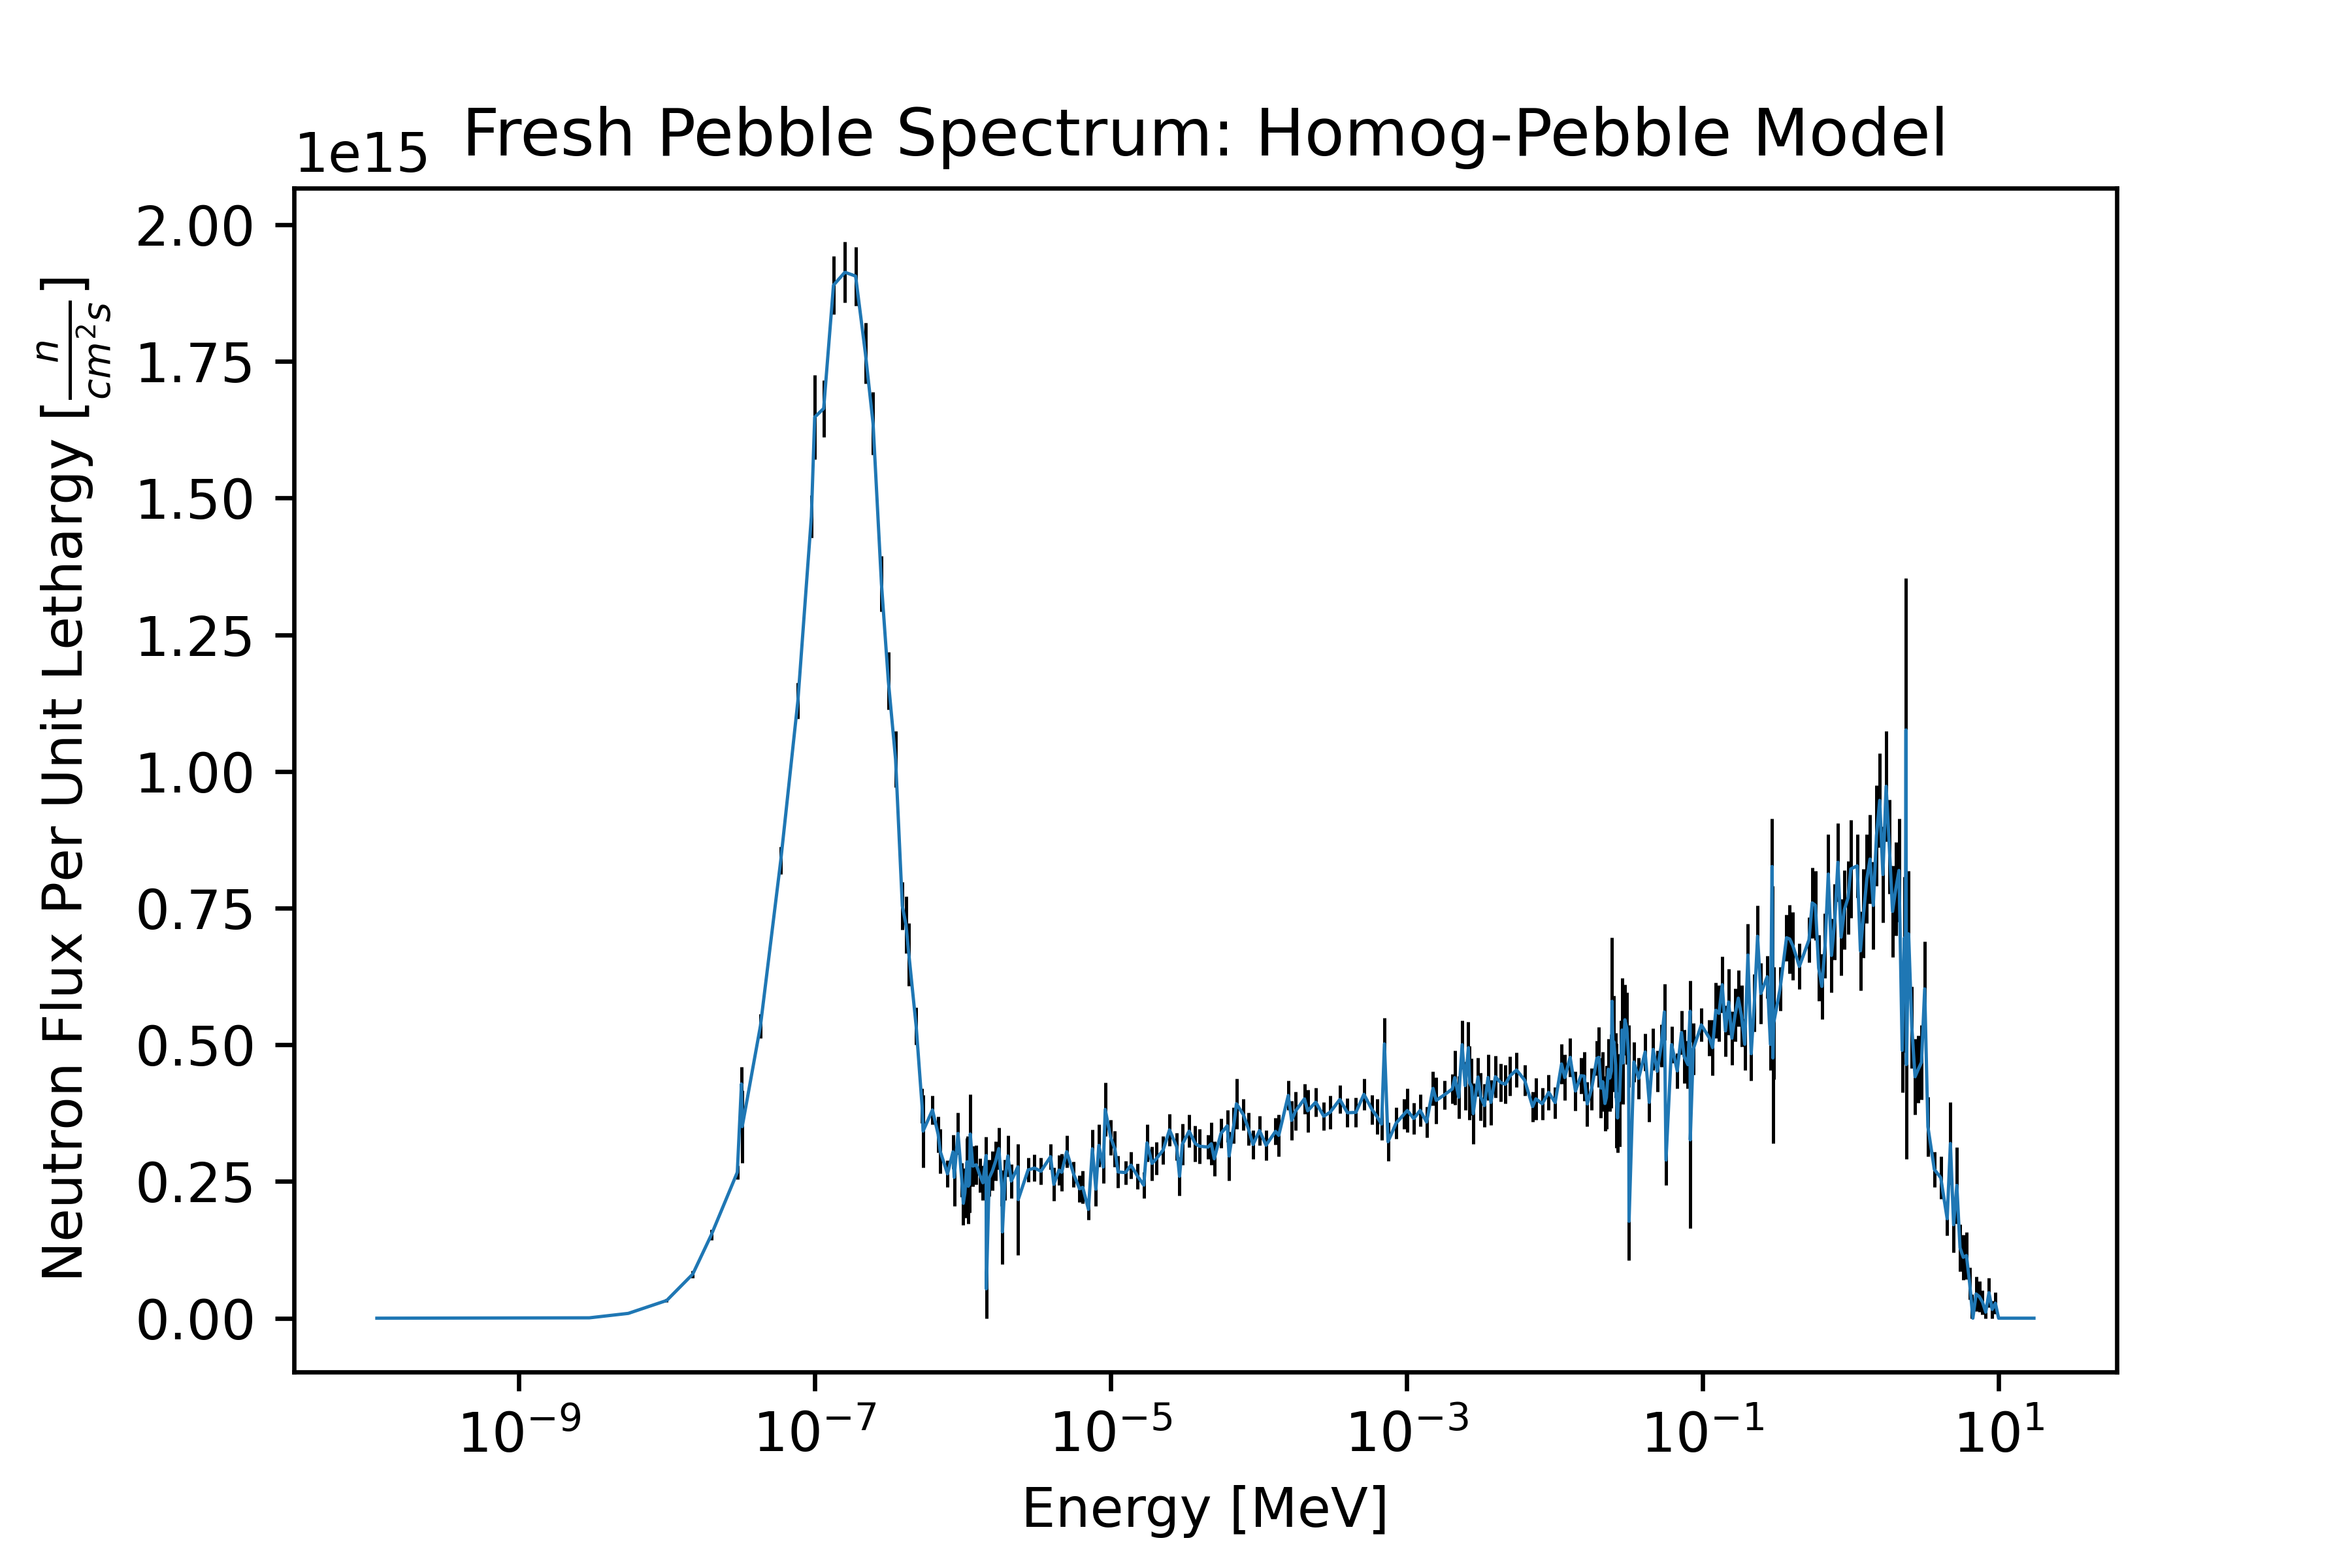
\includegraphics[width=0.95\linewidth]{figures/fresh_spec_homog}
  \caption{Lethargy Adjusted Neutron Flux Energy Spectrum in a Fresh Pebble for the Homogenized-Pebble Sangamon20}
  \label{fig:hom-fresh}
\end{figure}

\begin{figure}[H]
\centering
  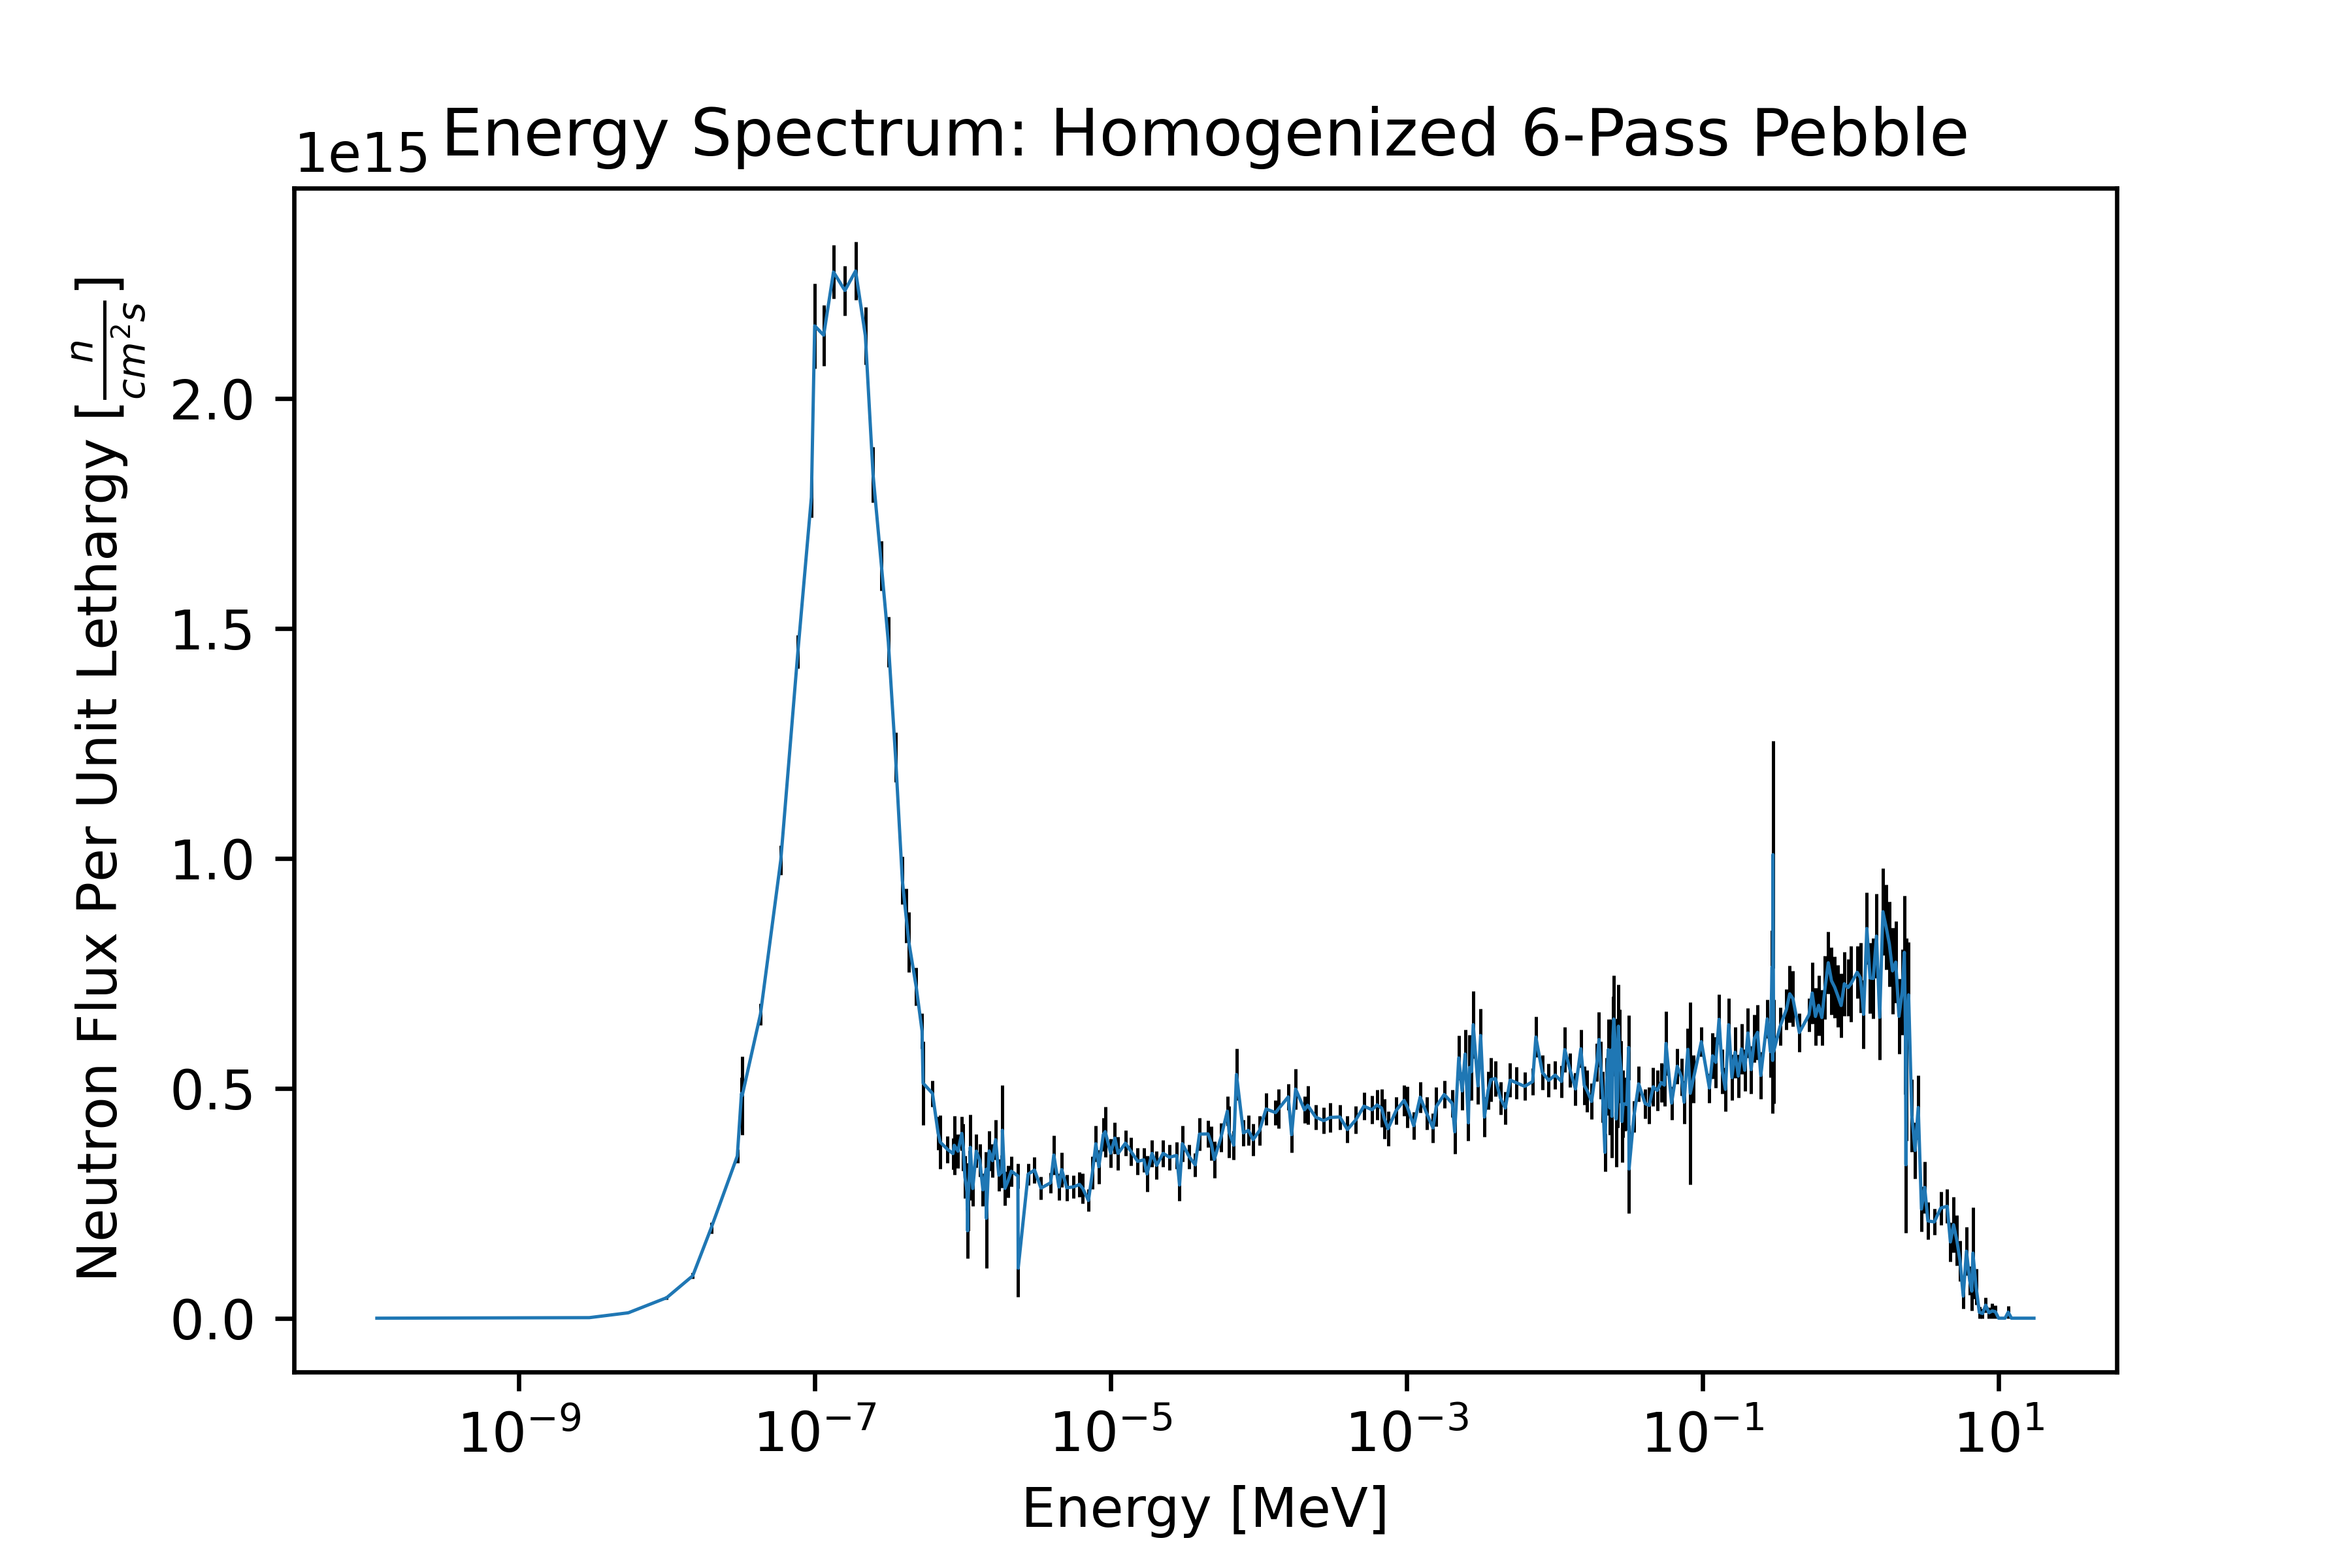
\includegraphics[width=0.95\linewidth]{figures/6_spec_homog}
  \caption{Lethargy Adjusted Neutron Flux Energy Spectrum in a Six-Pass Pebble for the Homogenized-Pebble Sangamon20}
  \label{fig:hom-six}
\end{figure}

\begin{figure}[H]
\centering
  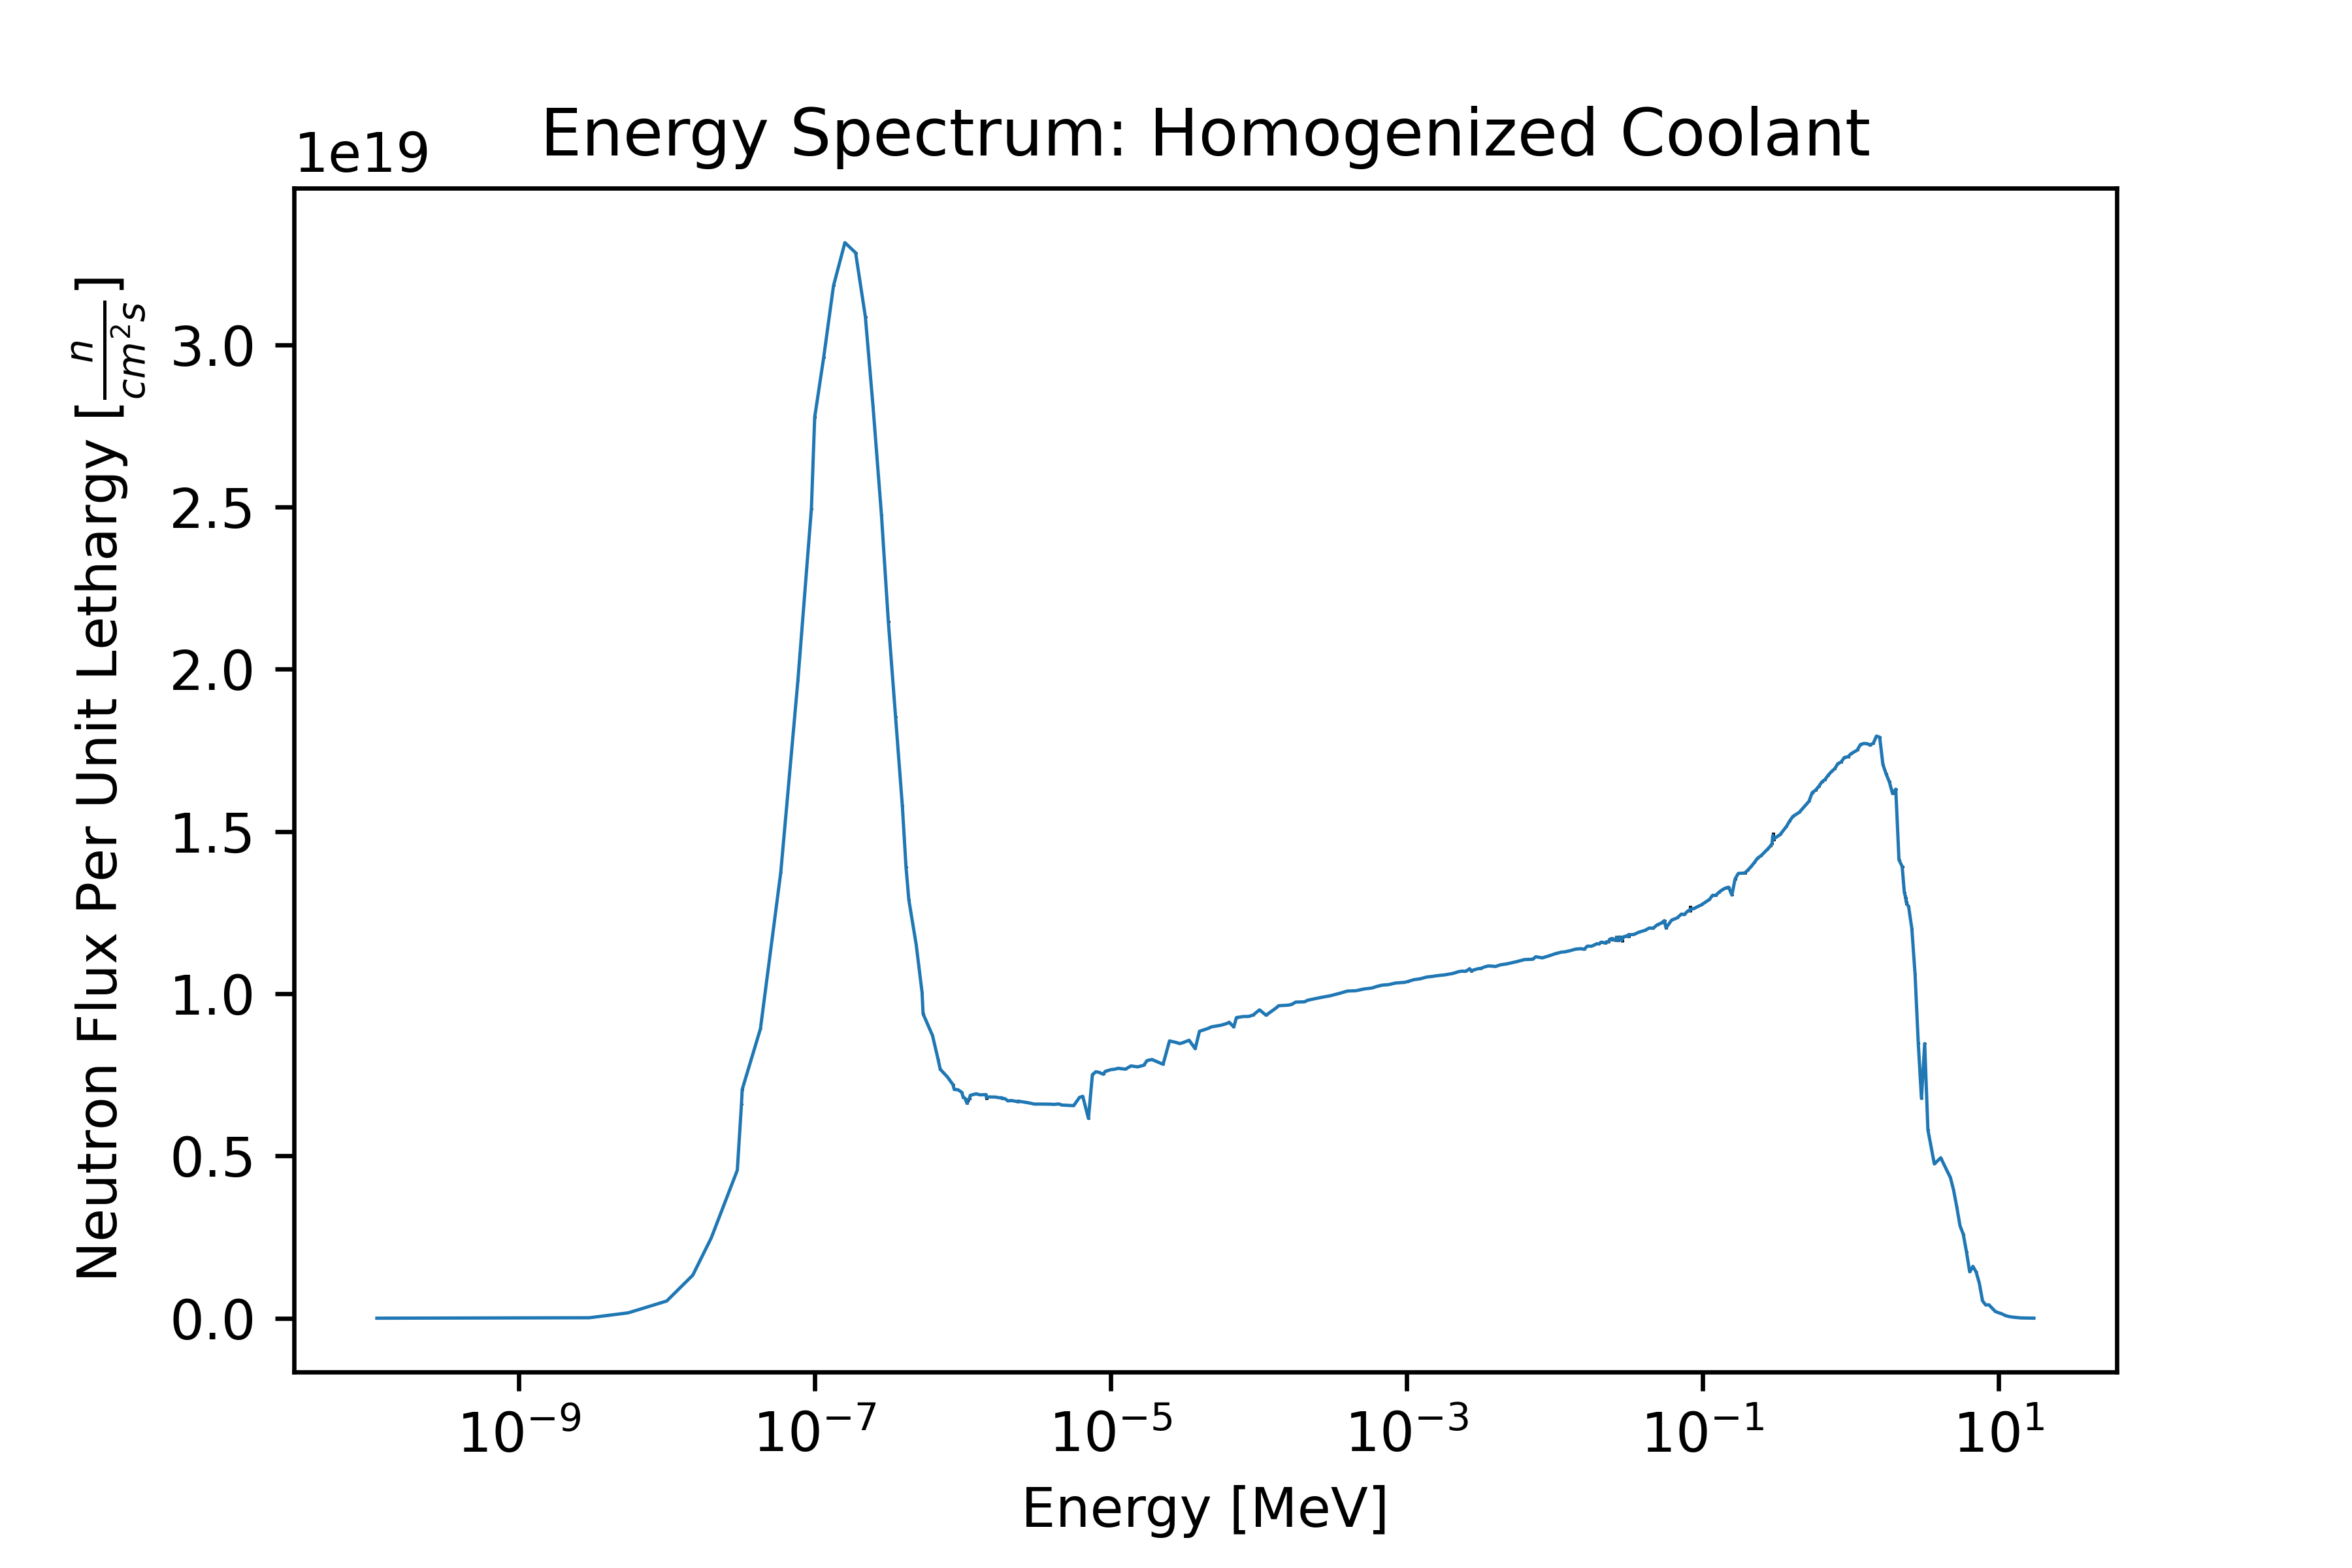
\includegraphics[width=0.95\linewidth]{figures/cool_spec_homog}
  \caption{Lethargy Adjusted Neutron Flux Energy Spectrum in the Coolant for the Homogenized-Pebble Sangamon20}
  \label{fig:hom-cool}
\end{figure}


The spectra for a randomly selected fresh and sixth-pass pebble are subject to the highest uncertainty of all the provided spectra in Figures \ref{fig:hom-core} through \ref{fig:hom-cool}, as a single pebble has a relatively small bin size, which means fewer particles contribute to the tally regions.  However, if coupled with the coolant spectra, Figure \ref{fig:hom-cool}, they provide a clearer look at the flux energy spectrum in the active core region.  We can see that, while the thermal energy of the fresh and six-pass pebbles are similar in shape and magnitude, the magnitude of the faster groups differ considerably.


\section{Effect of Homogenization}
\label{res-hom}

The results discussed previously use the assumption of a pebble that has the TRISO particles homogenized and blended with the rest of the pebble matrix in the region containing fuel.  However, homogenization can cause under-predictions of k-eff as much as 5-6\% \cite{brown_stochastic_2005}.  To test the impact of homogenization on Sangamon20, the heterogenization tests were performed.  These tests use an otherwise identical Sangamon20 model with explicitly modeled TRISO particles.  As a reminder, the isotopic compositions come from the same burnup simulation.  As such, the isotopic compositions between the homogenized and heterogenized simulations are identical.


\begin{figure}[H]
\centering

\begin{subfigure}{0.45\textwidth}
  \includegraphics[width=0.95\linewidth]{figures/het/het-r}
  \caption{Radial Cross Section at y=0}
  \label{fig:heta}
\end{subfigure}%
%
\begin{subfigure}{0.45\textwidth}
  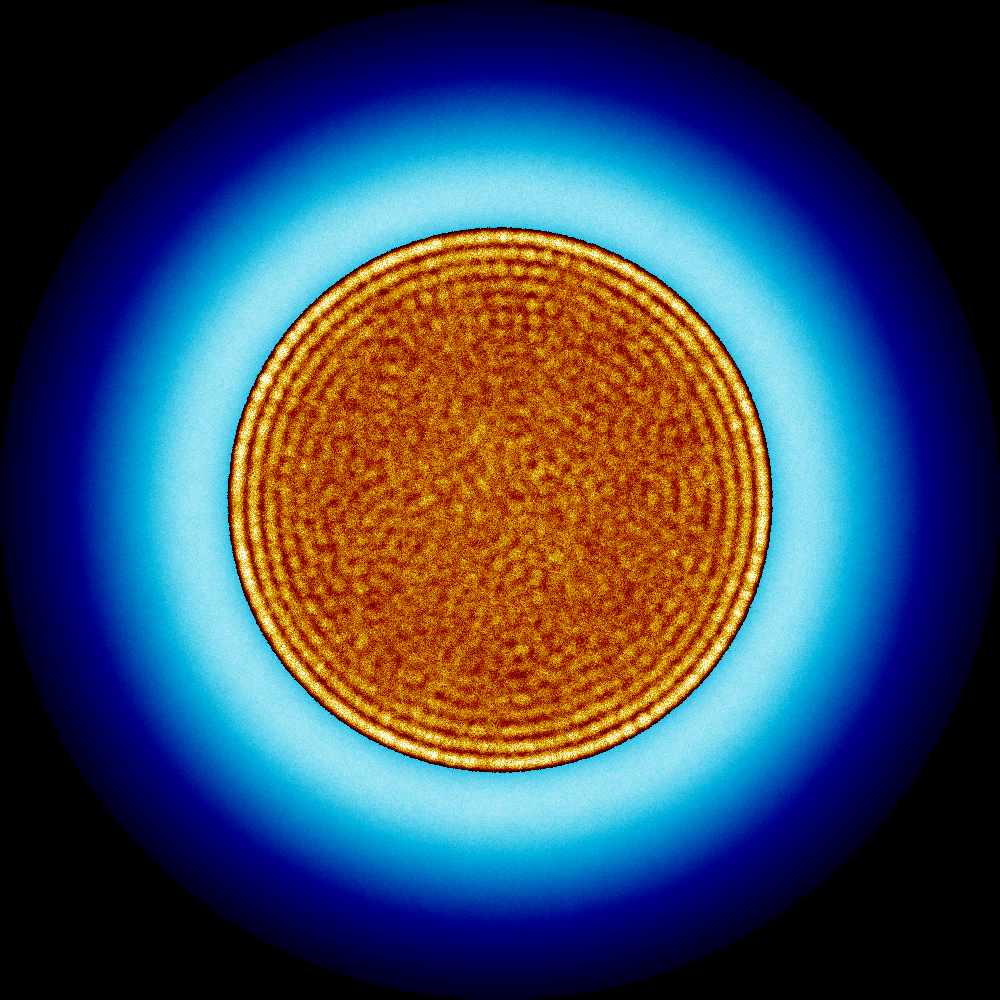
\includegraphics[width=0.95\linewidth]{figures/het/het-rm}
  \caption{Radial Mesh}
  \label{fig:hetb}
\end{subfigure}

\begin{subfigure}{0.45\textwidth}
  \includegraphics[width=0.95\linewidth]{figures/het/het-v}
  \caption{Axial Cross Section at z=0 }
  \label{fig:hetc}
\end{subfigure}
%
\begin{subfigure}{0.45\textwidth}
  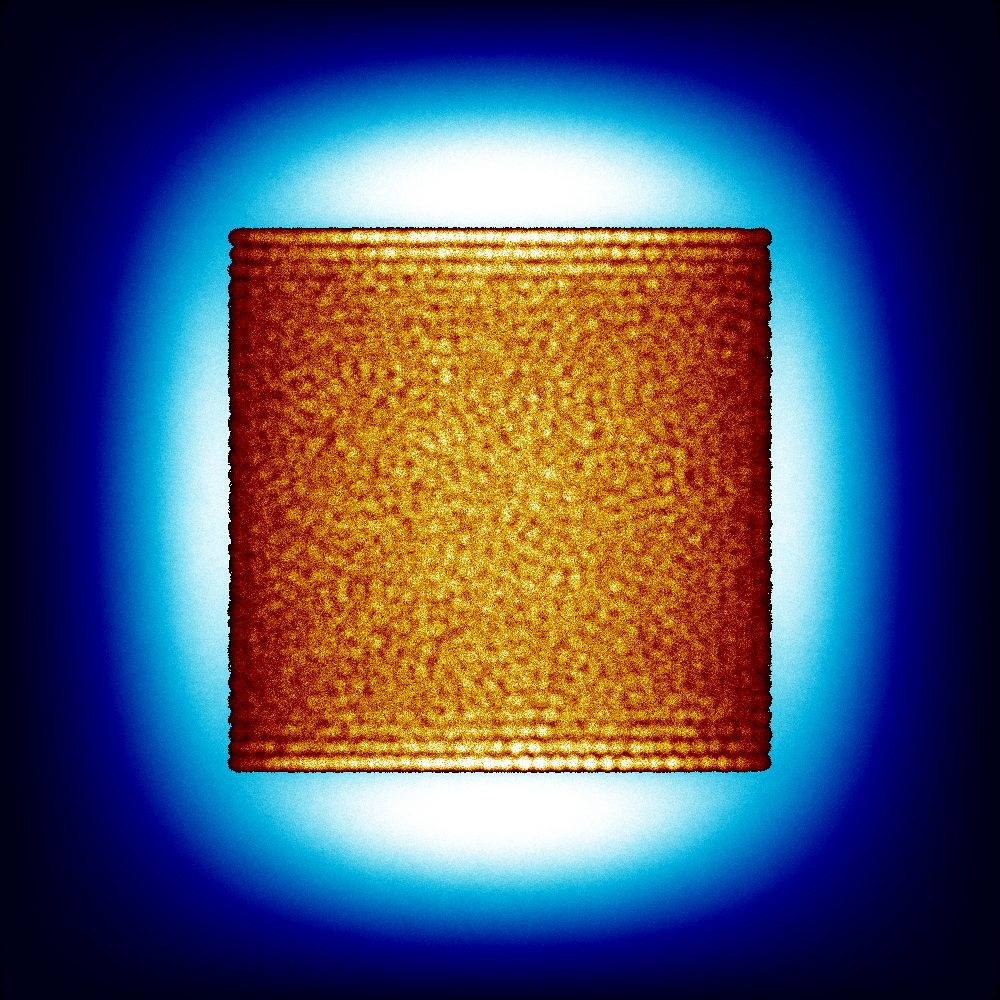
\includegraphics[width=0.95\linewidth]{figures/het/het-vm}
  \caption{Axial Mesh}
  \label{fig:hetd}
\end{subfigure}
%
\caption{Full Core Using Heterogenized Pebbles}
\label{fig:het}
\end{figure}

The heterogenized-TRISO model reported a $k_{eff}$ of $1.087 \pm 0.00032$.  This is significantly higher than the $k_{eff}$ reported for the control (homogenized-TRISO) model --- only $1.041 \pm 0.00054$.  In agreement with \cite{brown_stochastic_2005}, this is a difference of 4.23\%.  

Overall, the mesh result for the heterogenization test fission rate is much the same - the banding patterns are still present, if slightly less defined.  While Figure \ref{fig:het} best serves as a qualitative visualization aid, Figures \ref{fig:het-det-xy}, \ref{fig:het-det-z}, \ref{fig:het-plane-therm}, and \ref{fig:het-plane-fast} support this in a more quantitative manner.  These figures give the shape and magnitude of the fluxes, which \ref{fig:het} cannot.


\begin{figure}[H]
\centering

\begin{subfigure}{0.9\textwidth}
  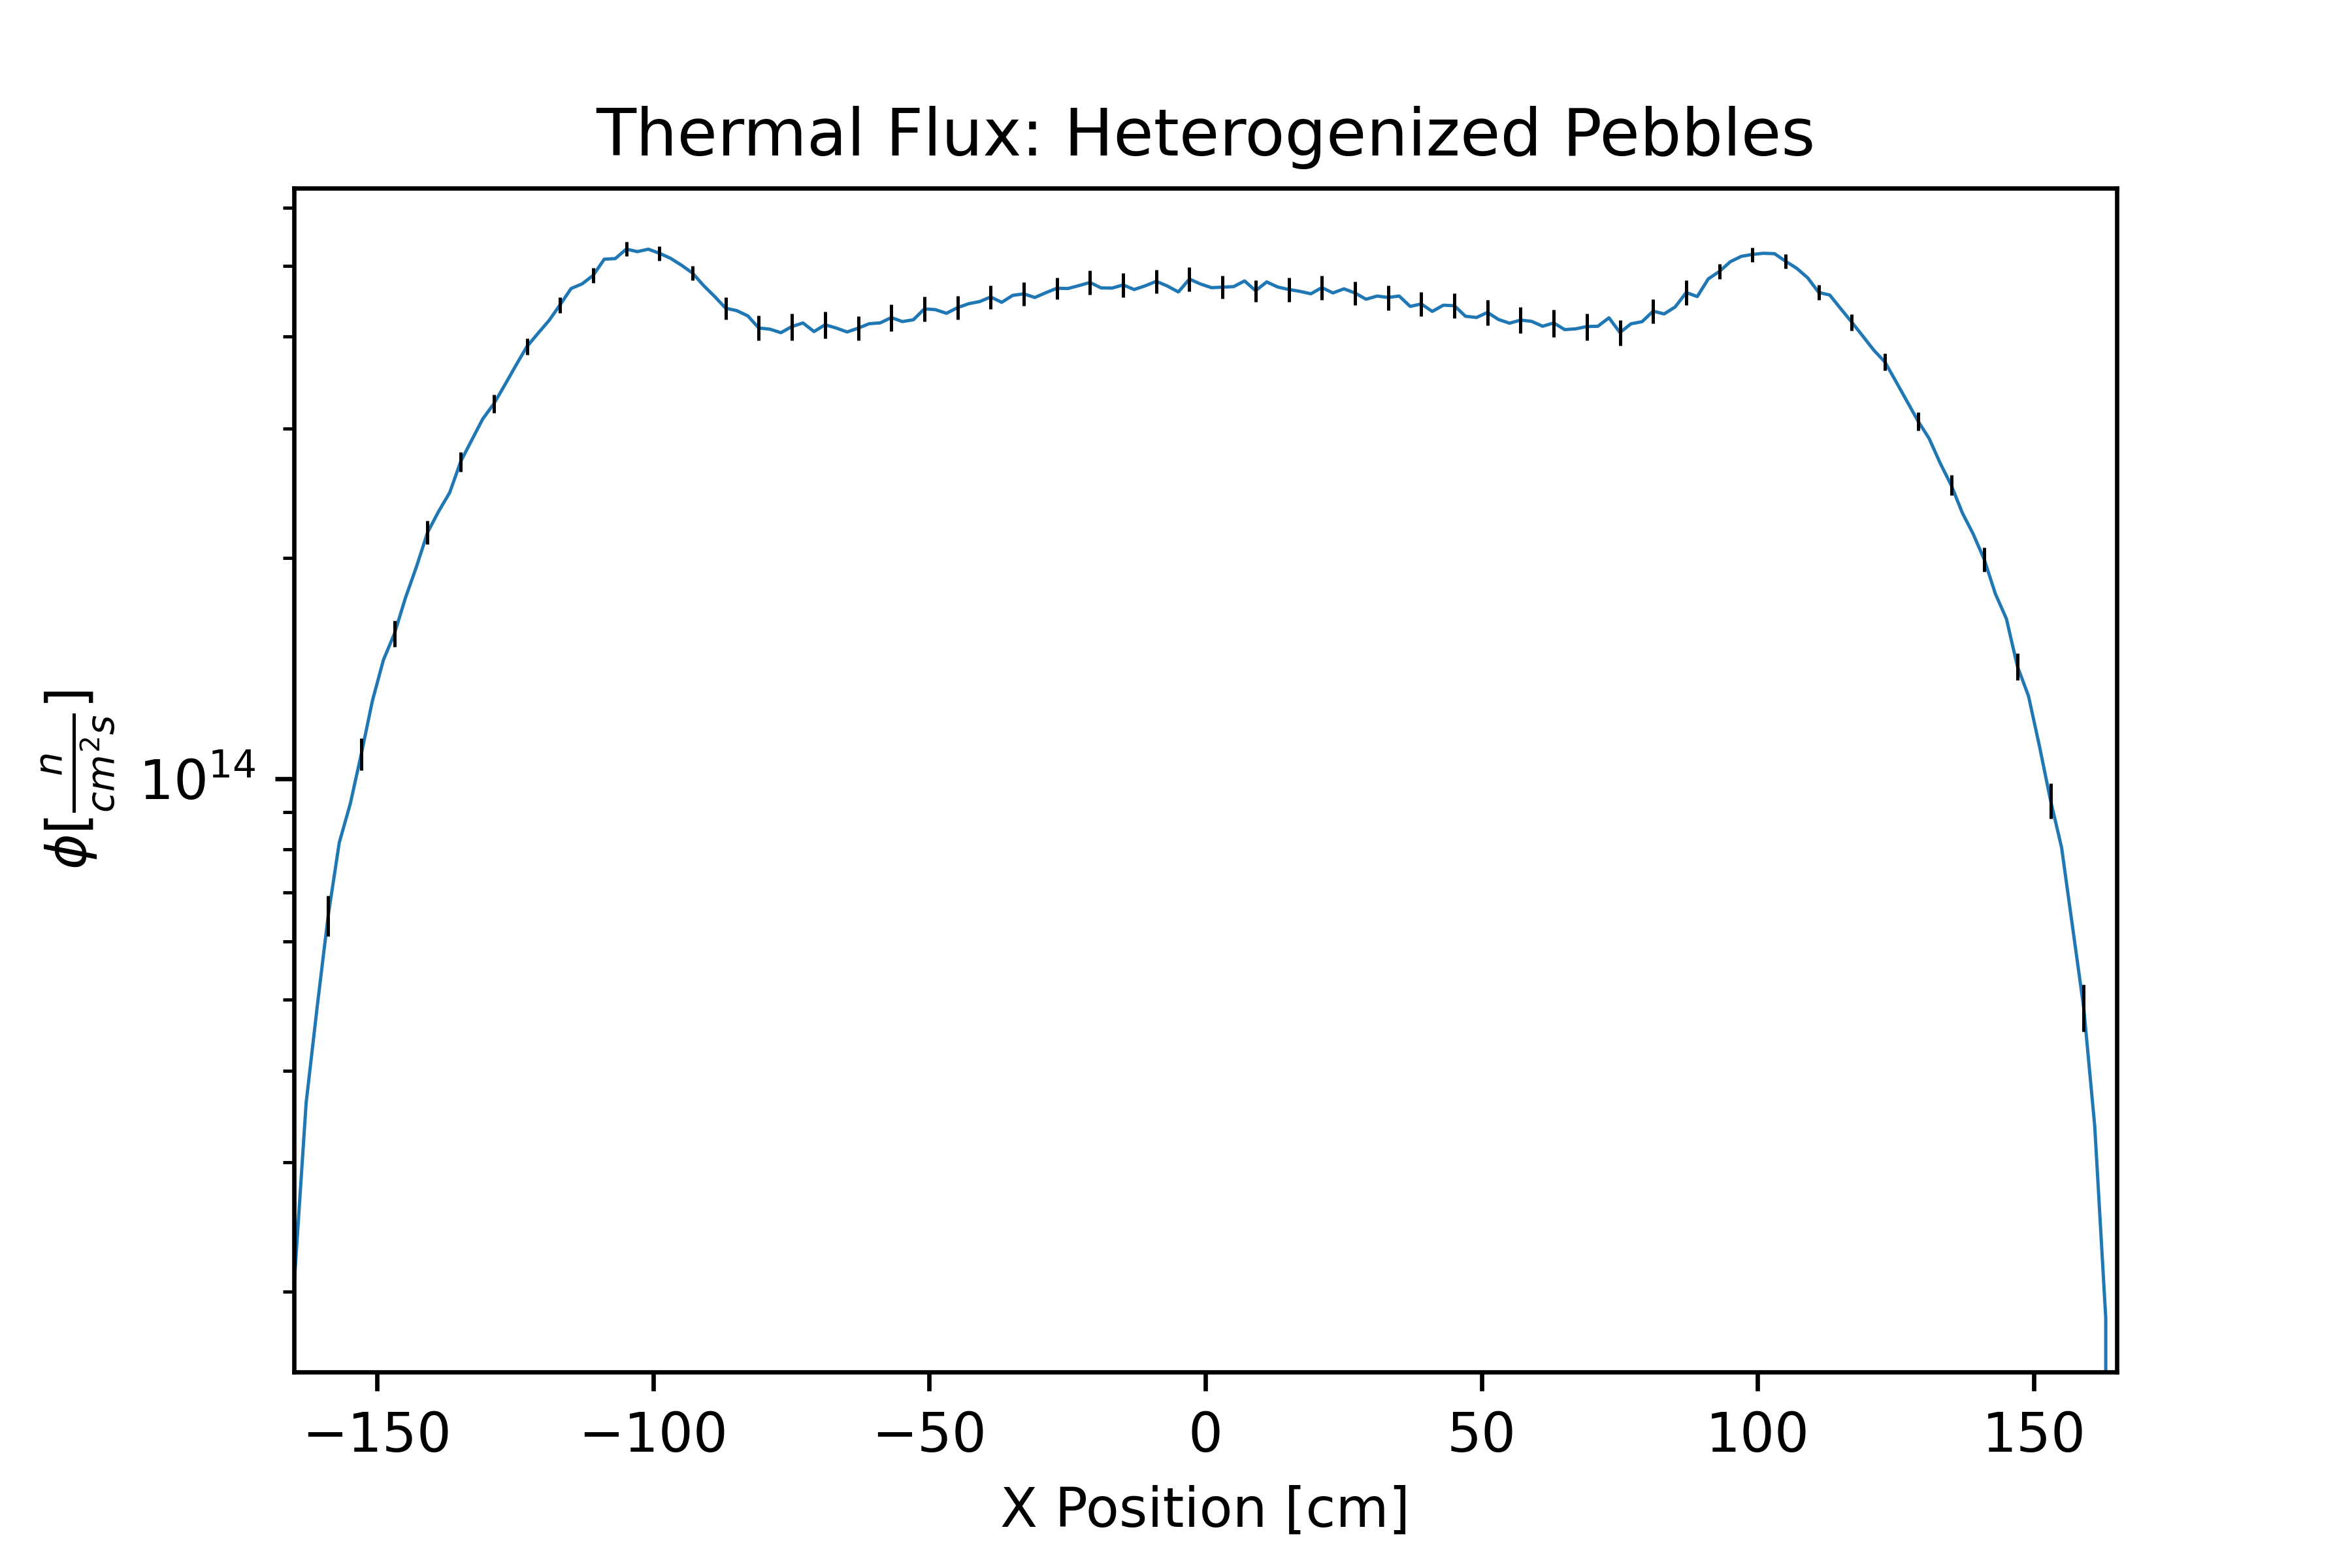
\includegraphics[width=0.95\linewidth]{figures/therm_flux_het.png}
  \caption{Thermal Flux}
  \label{fig:het-det-xy-therm}
\end{subfigure}%

\caption{Radial Thermal and Fast Flux Profiles: Heterogenized Pebbles}
\end{figure}

\begin{figure}[H]\ContinuedFloat
\centering

\begin{subfigure}{0.9\textwidth}
  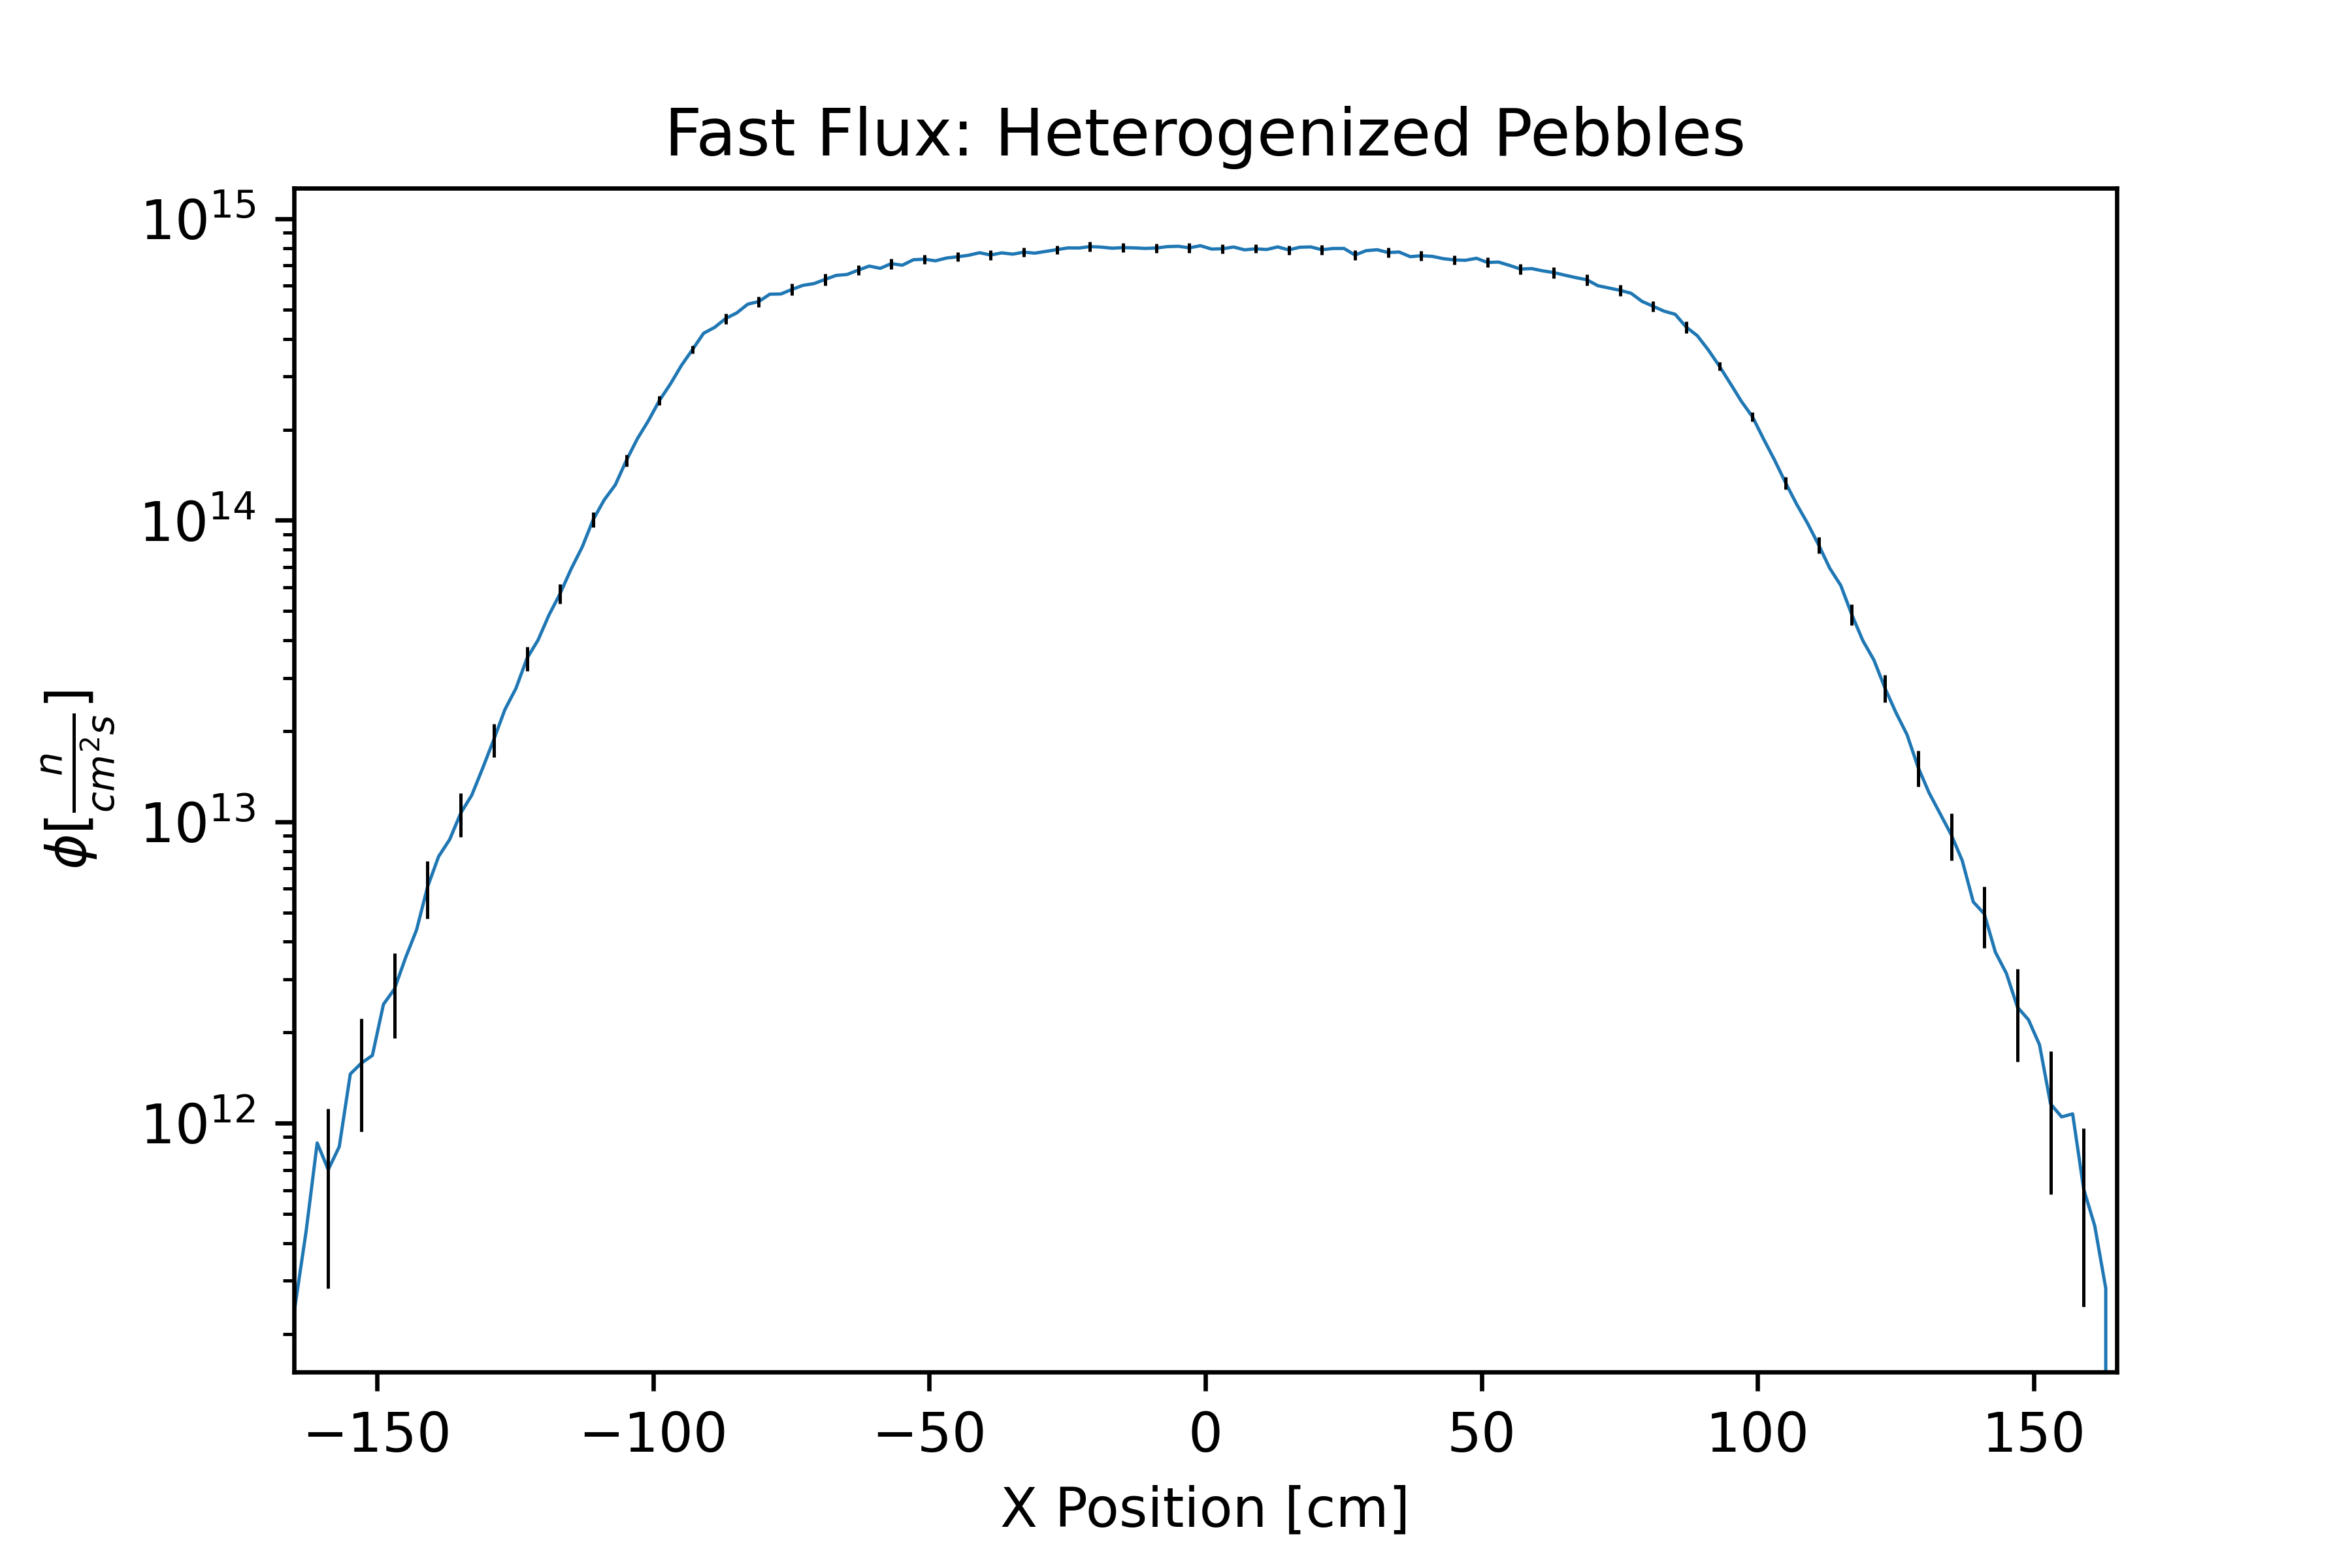
\includegraphics[width=0.95\linewidth]{figures/fast_flux_het.png}
  \caption{Fast Flux}
  \label{fig:het-det-xy-fast}
\end{subfigure}


\caption{Radial Thermal and Fast Flux Profiles: Heterogenized Pebbles (cont.)}
\label{fig:het-det-xy}
\end{figure}

Compared with the homogenized Sangamon20, the heterogenized core reports a slightly lower neutron current at the outer edge of the reflector, at $5.718\times10^{11} \pm 5.032\times10^{08}$, an absolute difference of approximately $2.00\times10^{09}$, which corresponds to a relative difference of 0.35\%.  The heterogenized model otherwise shows a similar flux profile to the homogenized model (see Figure \ref{fig:diff-flux}), and experiences a similar level of uncertainty in the outer edges of the reflector for the fast flux profiles, likely due to the significant thermalization of neutrons by that point in the reflector --- which results in fewer fast neutrons contributing to outer region tallies.


\begin{figure}[H]
\centering

  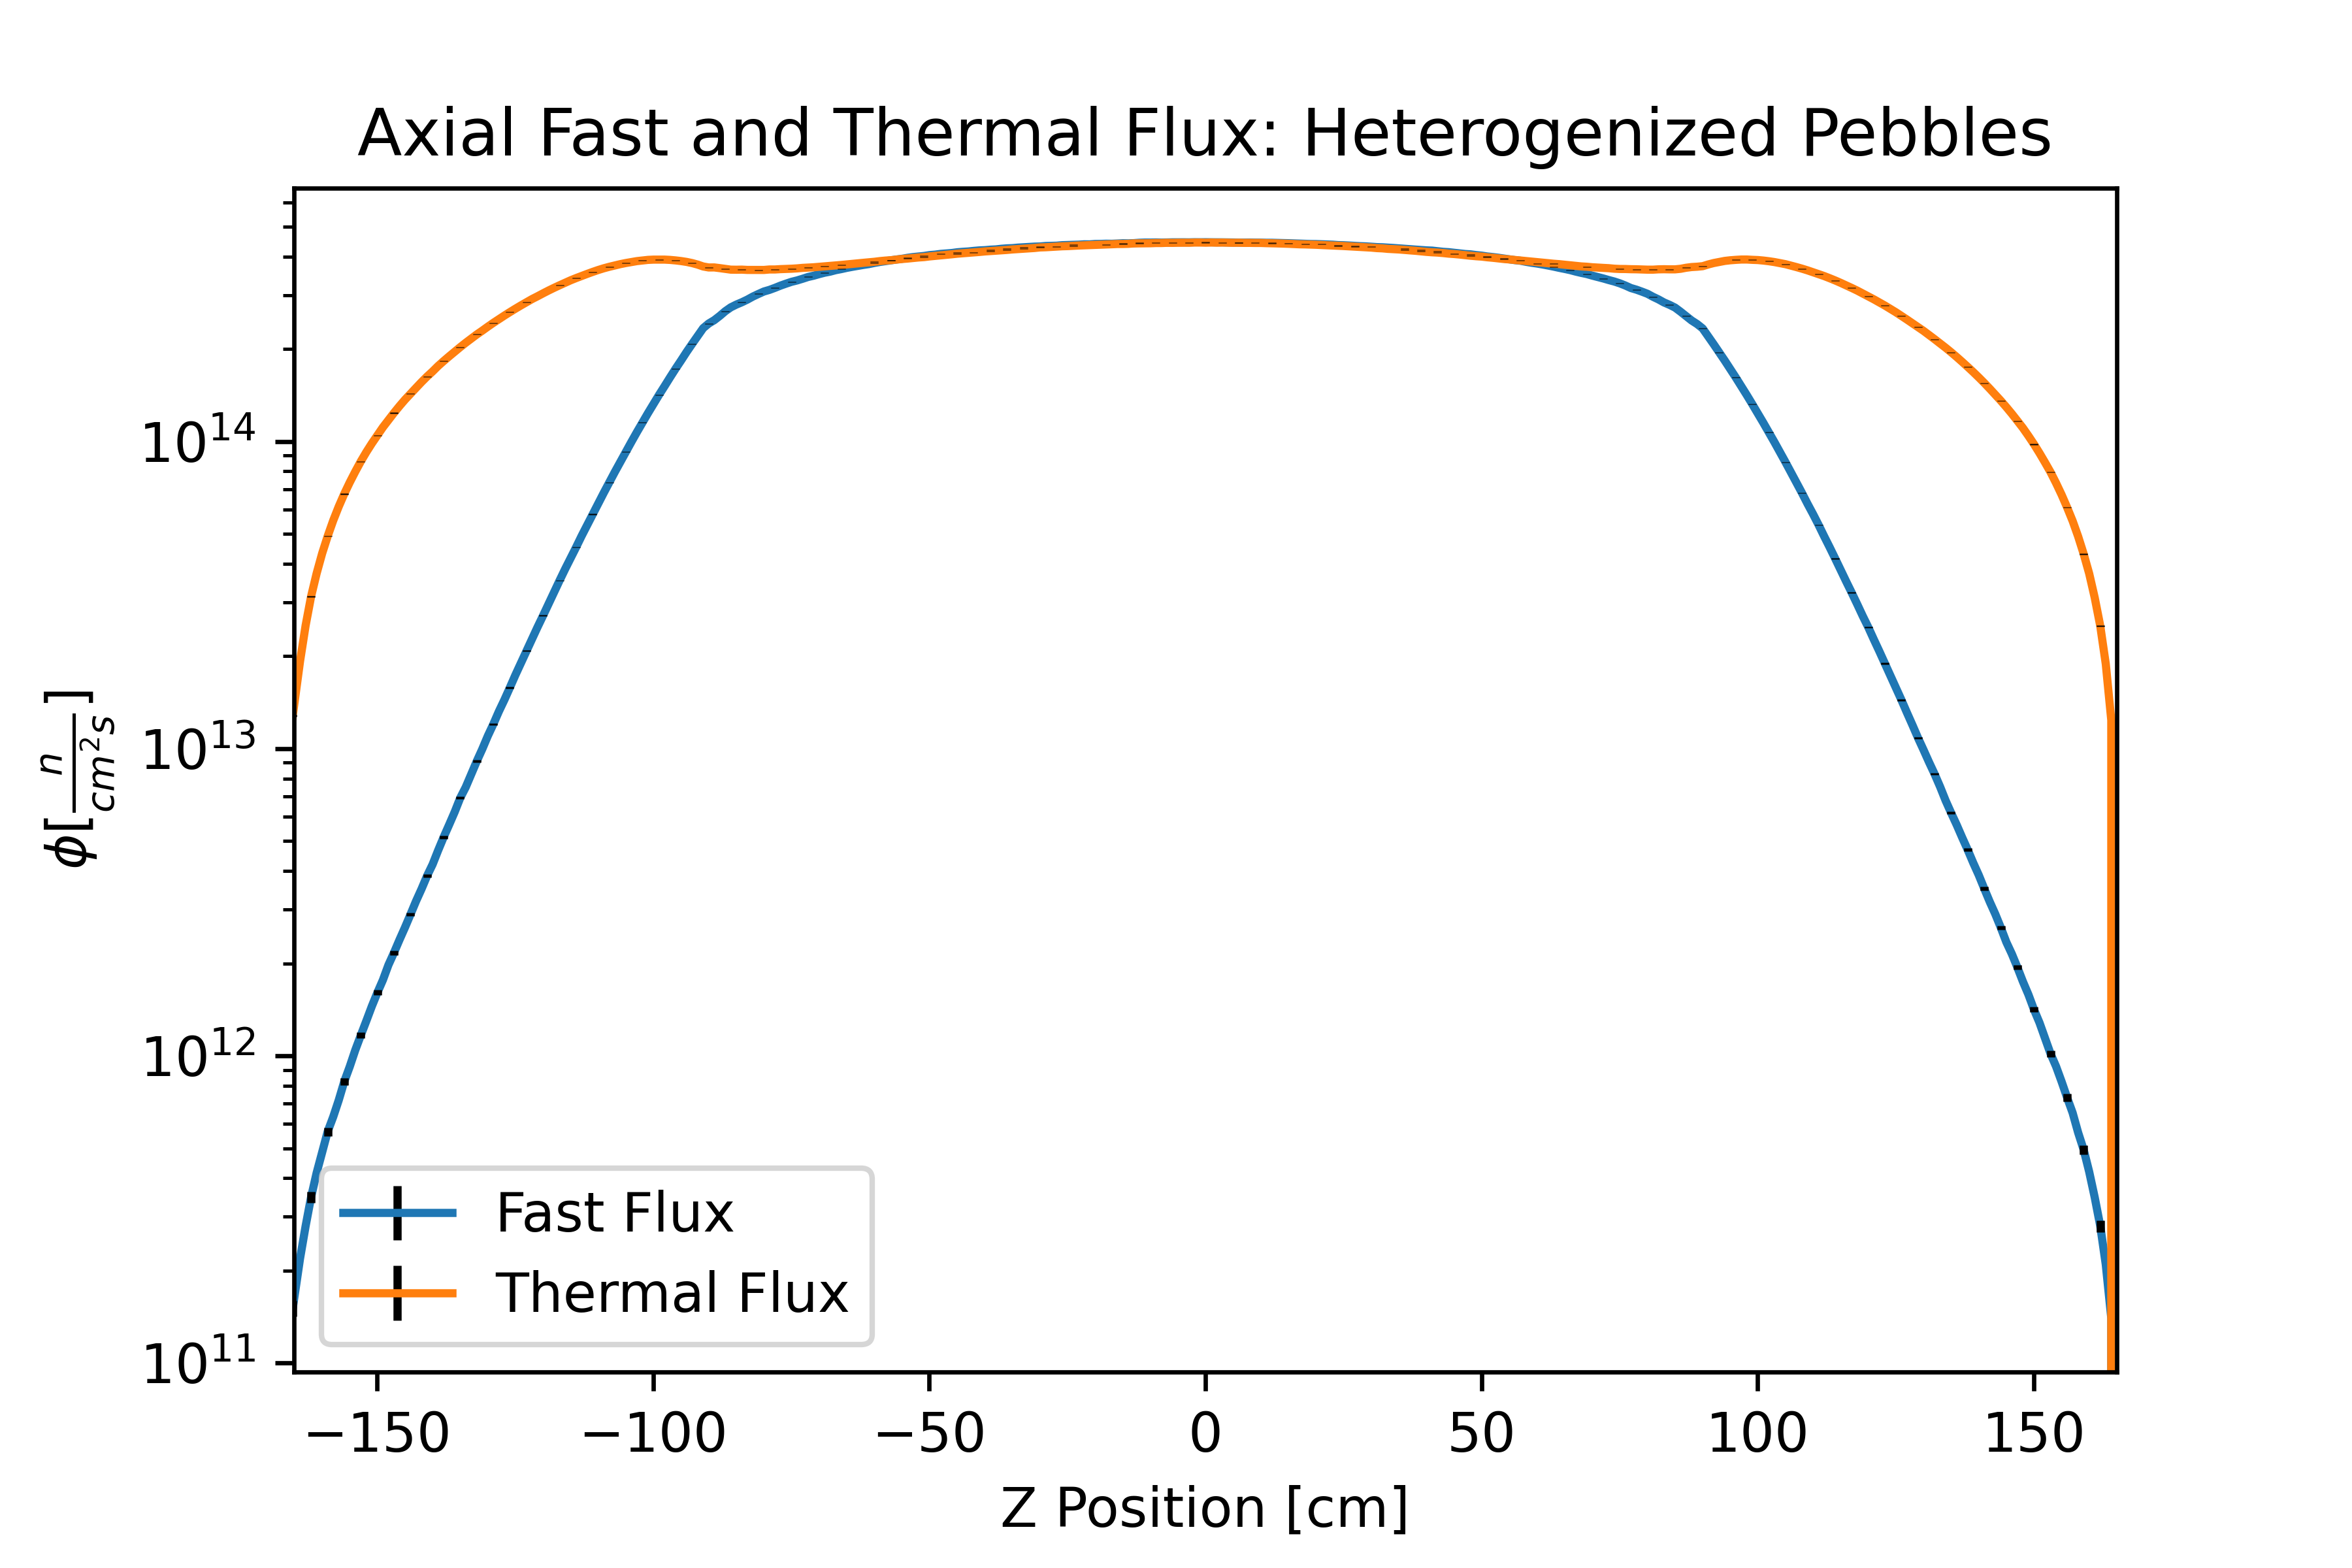
\includegraphics[width=0.95\linewidth]{figures/fast_therm_flux_het_z.png}

\caption{Axial Thermal and Fast Flux Profiles along the Centerline in Sangamon20: Heterogenized Pebbles}
\label{fig:het-det-z}
\end{figure}


\begin{figure}[H]
\centering

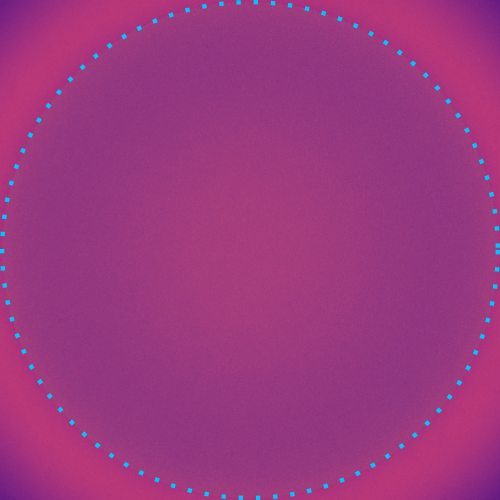
\includegraphics[width=0.95\linewidth]{figures/therm_xy_plane_het_er.png}
\caption{Thermal Flux in xy Plane in Sangamon20: Heterogenized Pebbles.  The dotted line annotation marks the boundary between the active core and the graphite reflector.}
\label{fig:het-plane-therm}

\end{figure}

\begin{figure}[H]
\centering

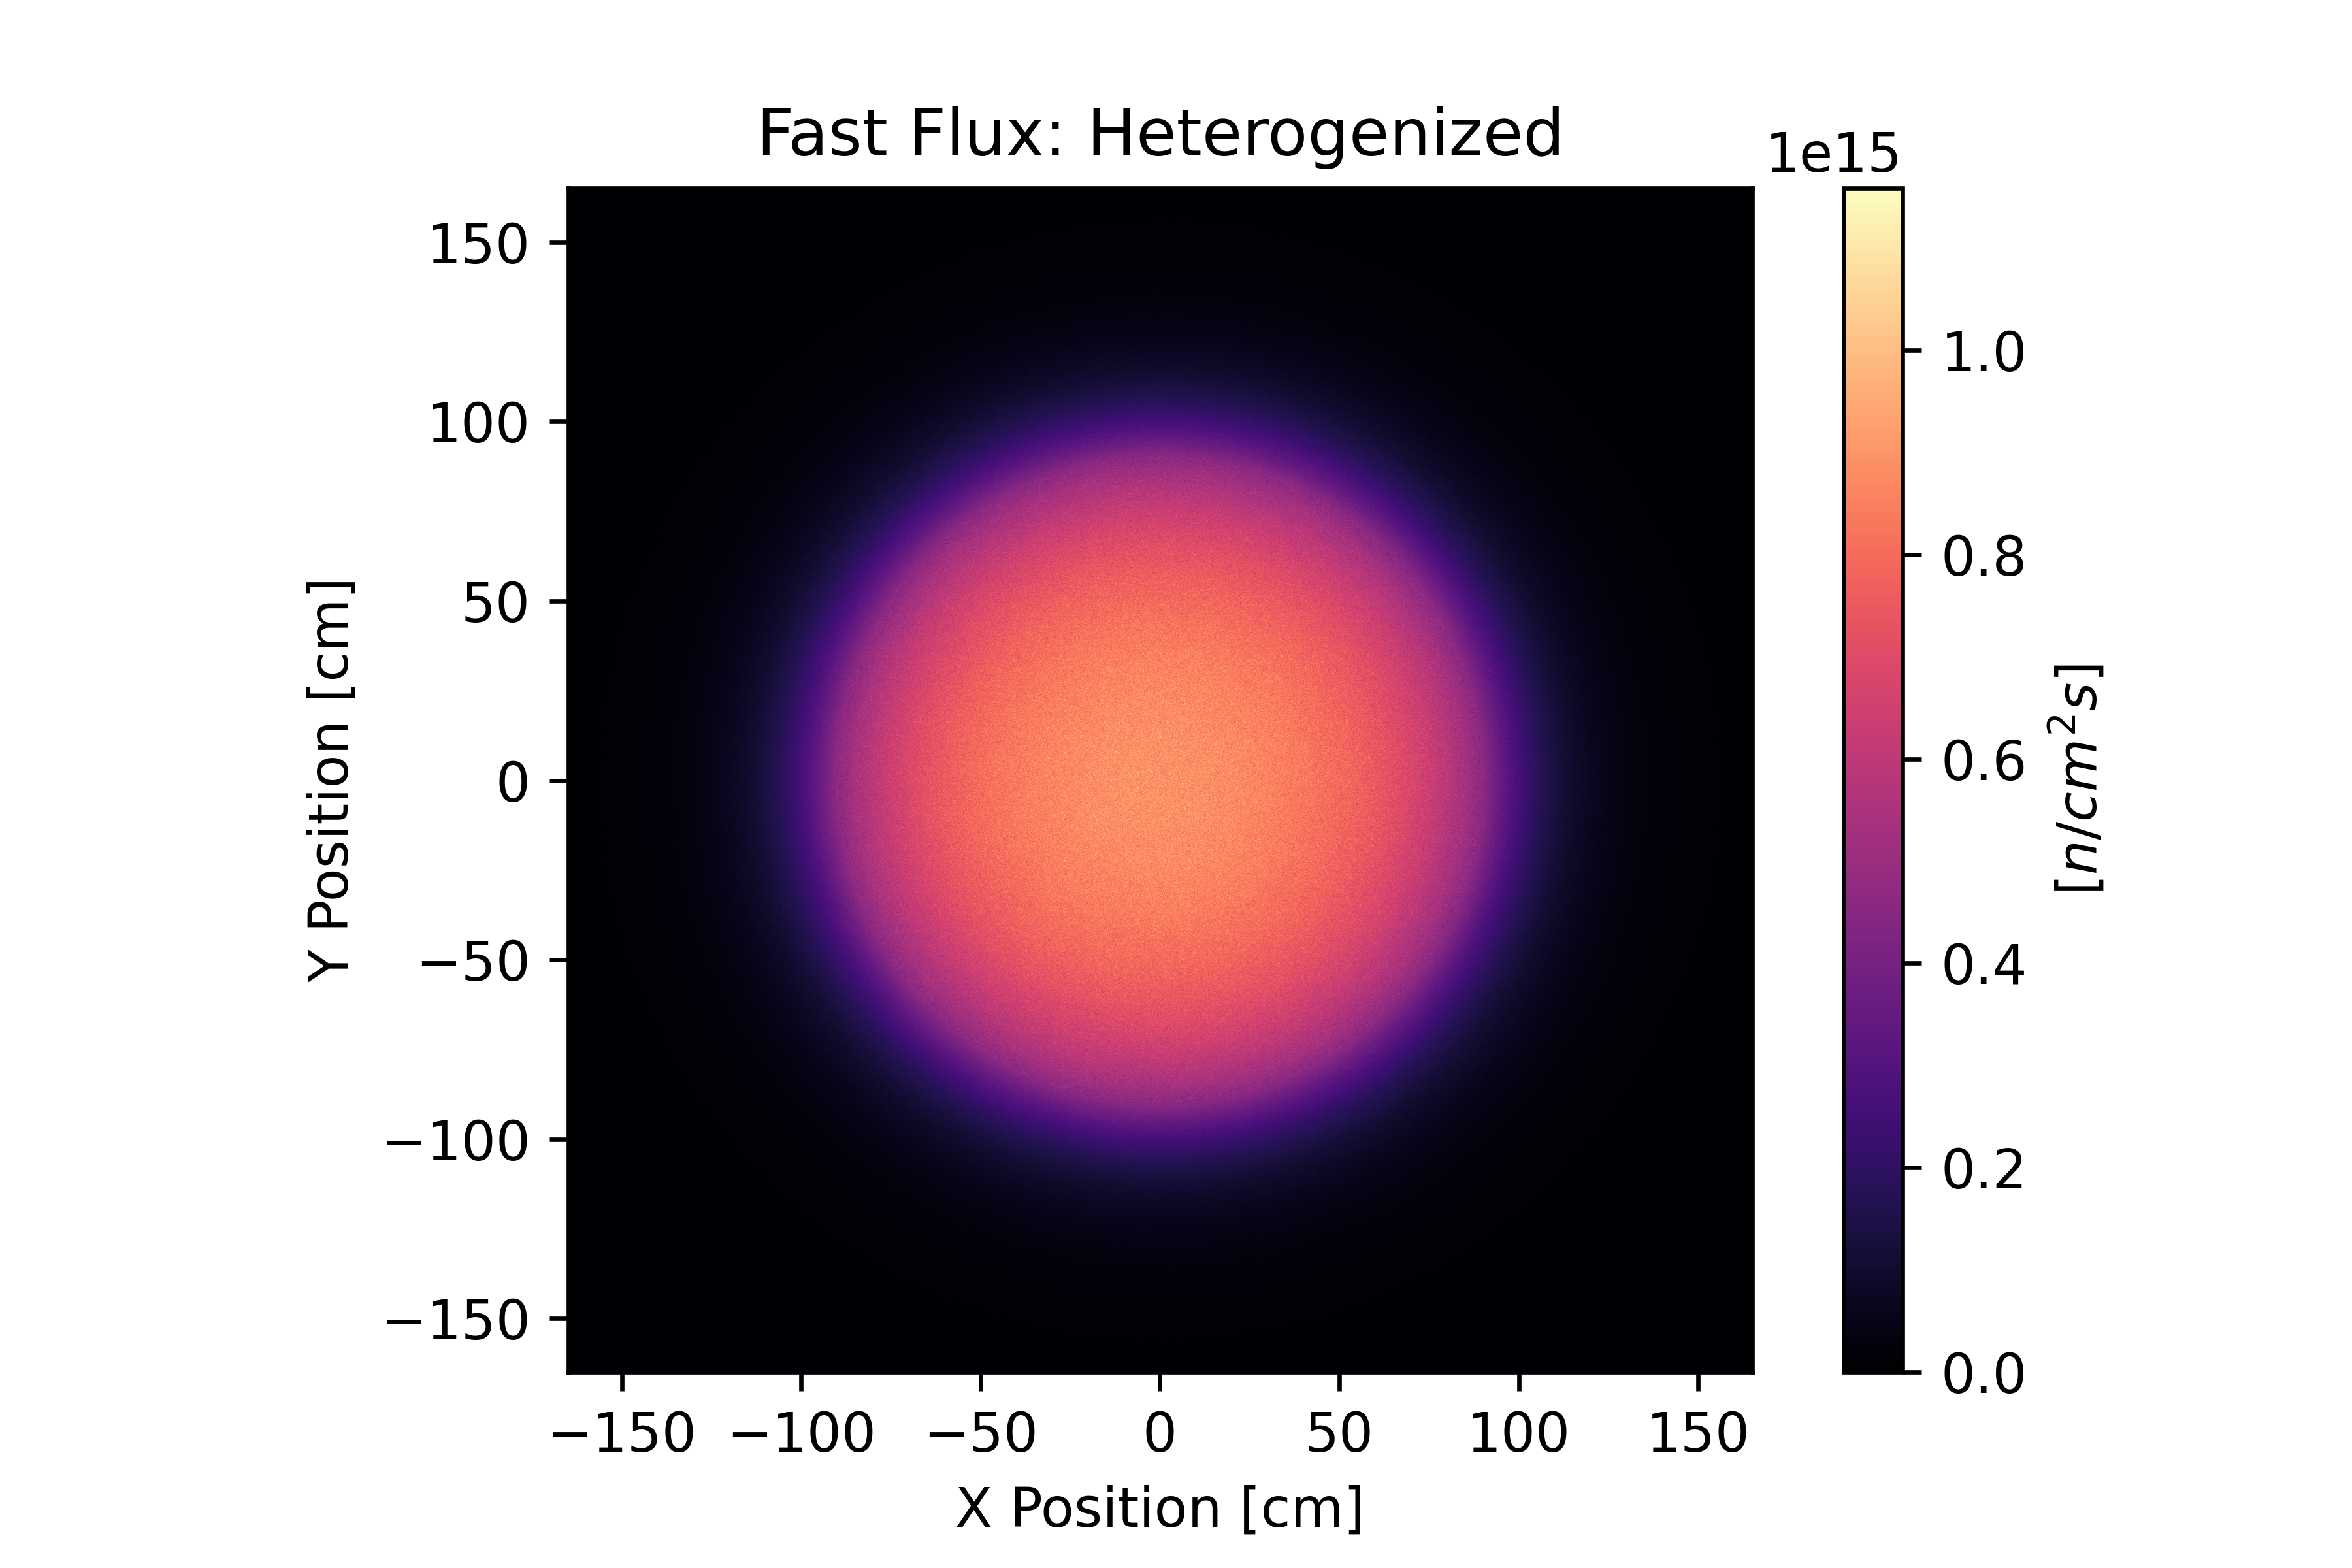
\includegraphics[width=0.95\linewidth]{figures/fast_xy_plane_het_er.png}
\caption{Fast Flux in xy Plane in Sangamon20: Heterogenized Pebbles.  The dotted line annotation marks the boundary between the active core and the graphite reflector.}
\label{fig:het-plane-fast}

\end{figure}

Compared with Figures  \ref{fig:het-plane-therm} and \ref{fig:het-plane-fast}, the edge pebble bands are much less distinct.  This is because the homogenized pebbles have the fissile material spread over the entirety of the 2.5 cm radius fueled center.  The heterogenized pebbles, meanwhile, may have the same number of fissile atoms, but the concentrate the regions capable of fission in the TRISO kernel.  The rest of the pebble consists of its graphite matrix.


\begin{figure}[H]
\centering

\begin{subfigure}{0.95\textwidth}
  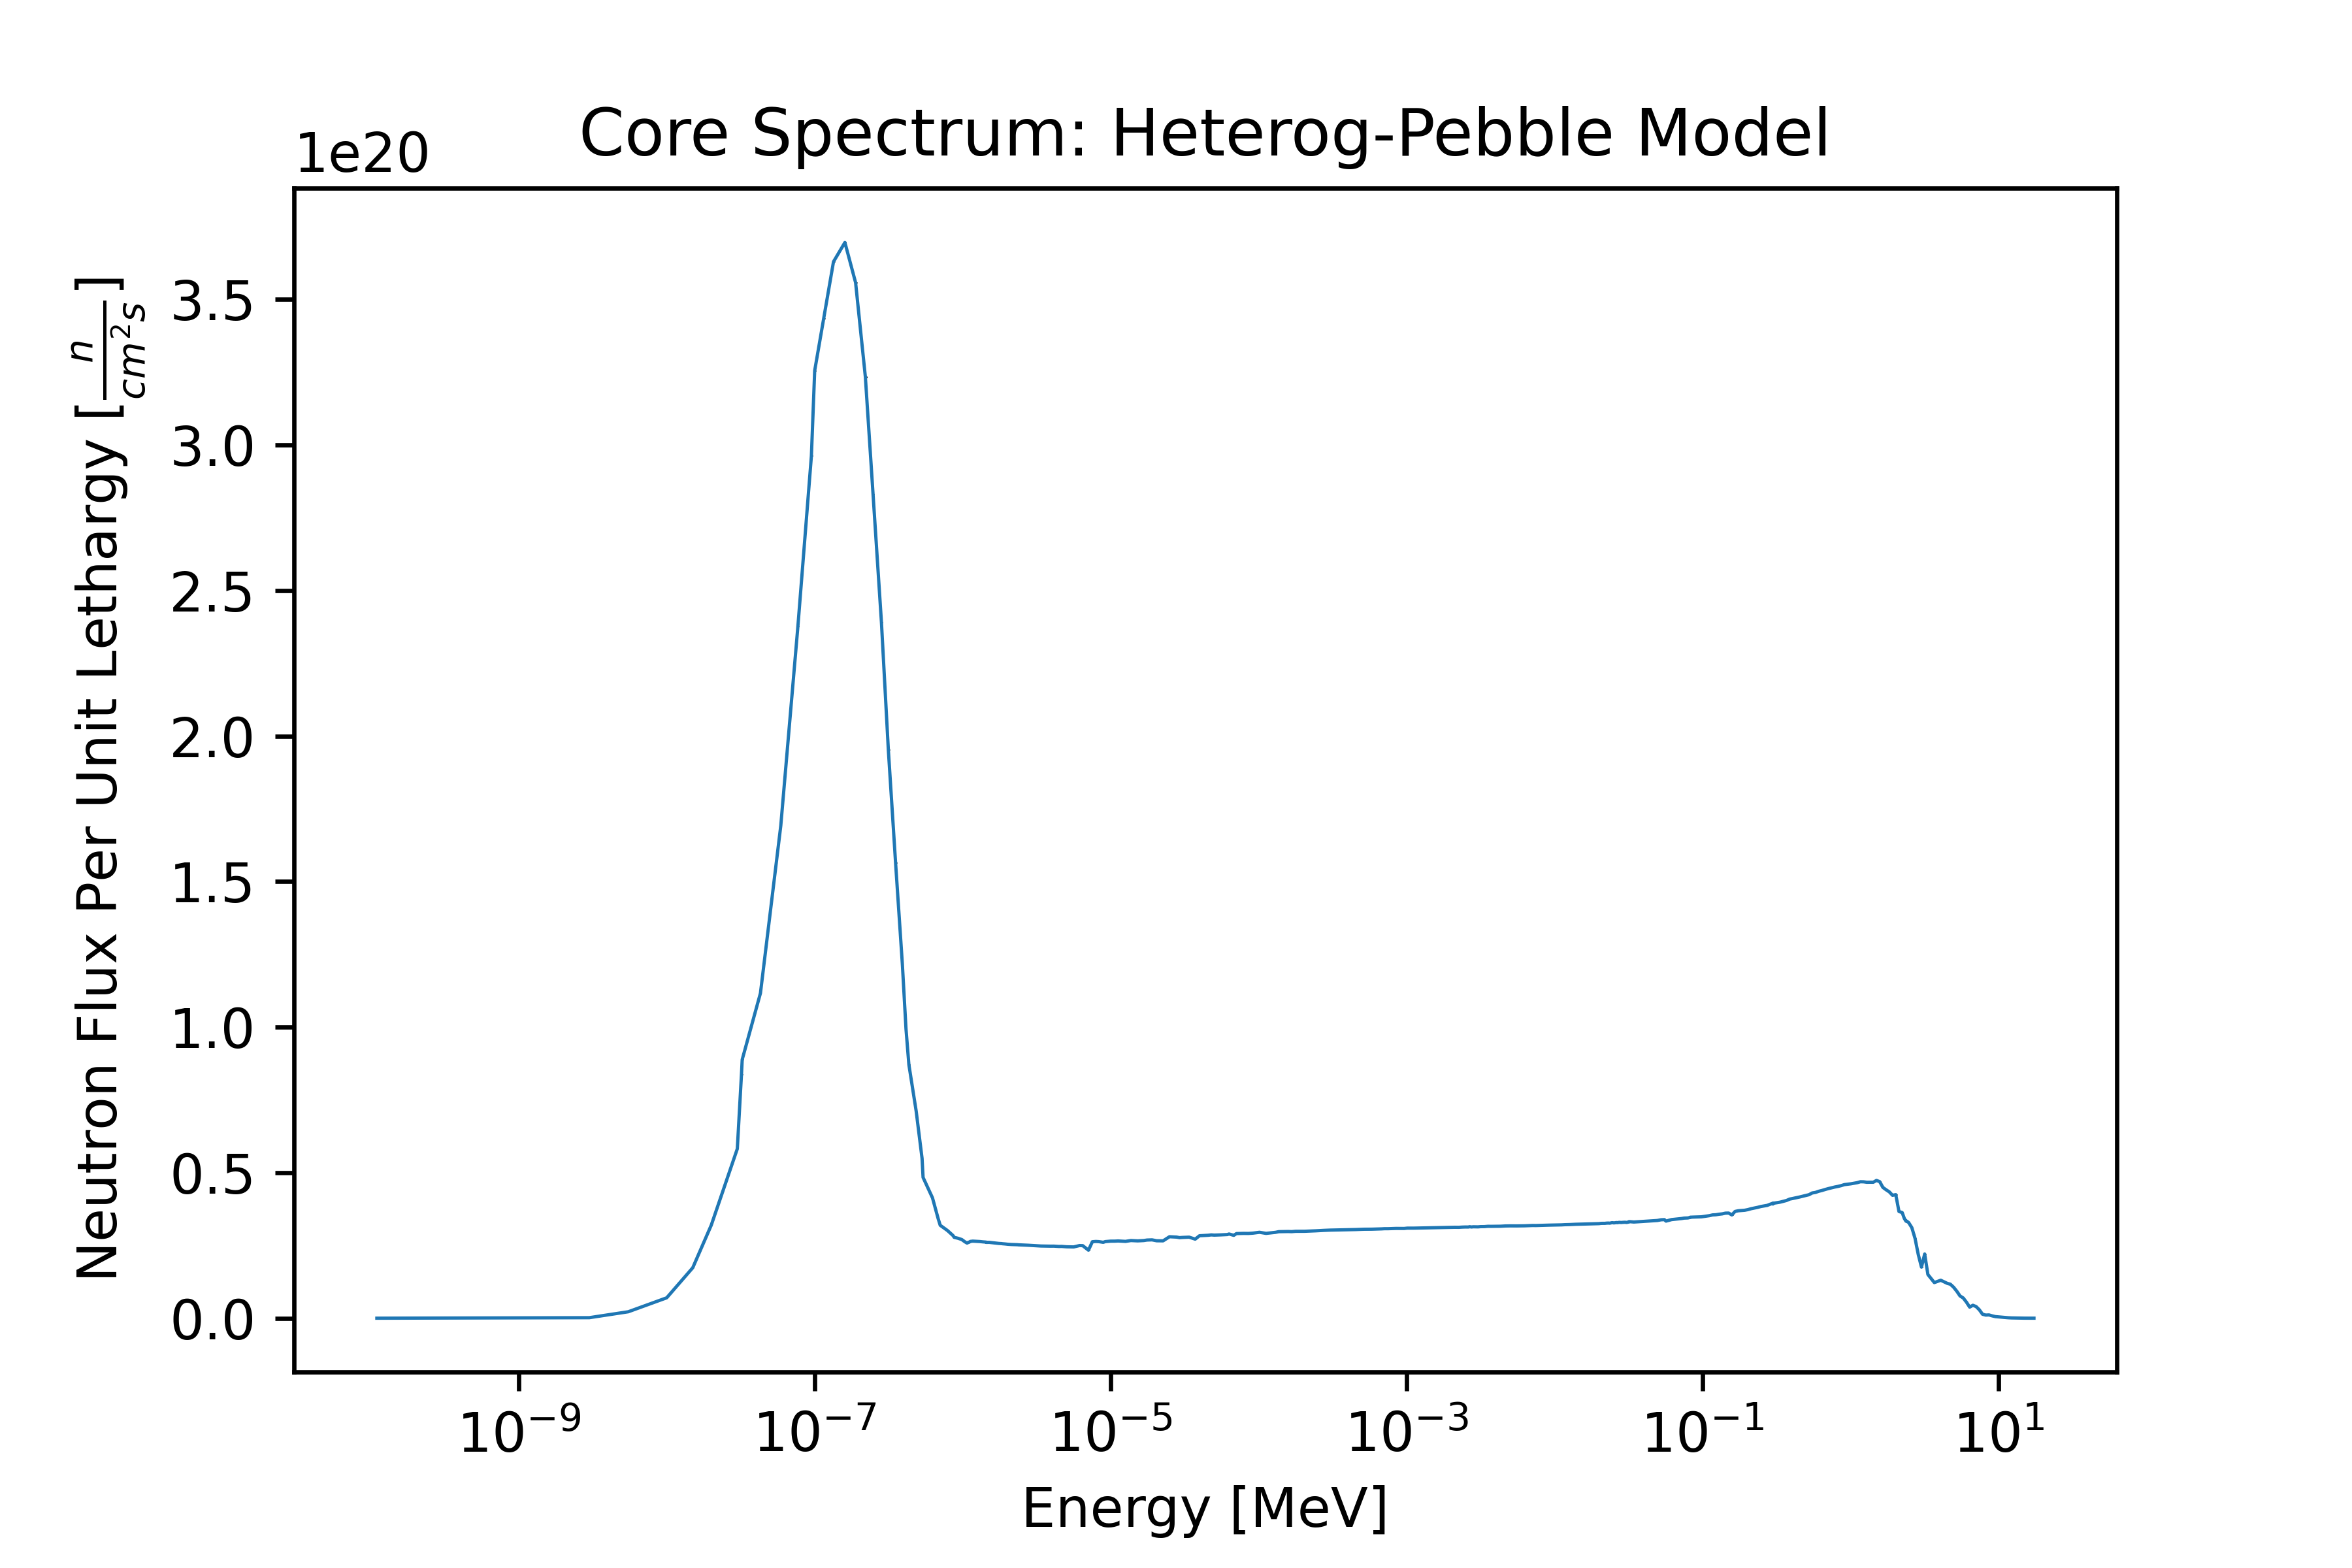
\includegraphics[width=0.95\linewidth]{figures/core_spec_het}
  \caption{Core Spectrum}
  \label{fig:het-core}
\end{subfigure}%

\caption{Lethargy Adjusted Neutron Flux Energy Spectra: Core Using Heterogenized Pebbles}
\end{figure}

\begin{figure}[H]\ContinuedFloat
\centering

\begin{subfigure}{0.95\textwidth}
  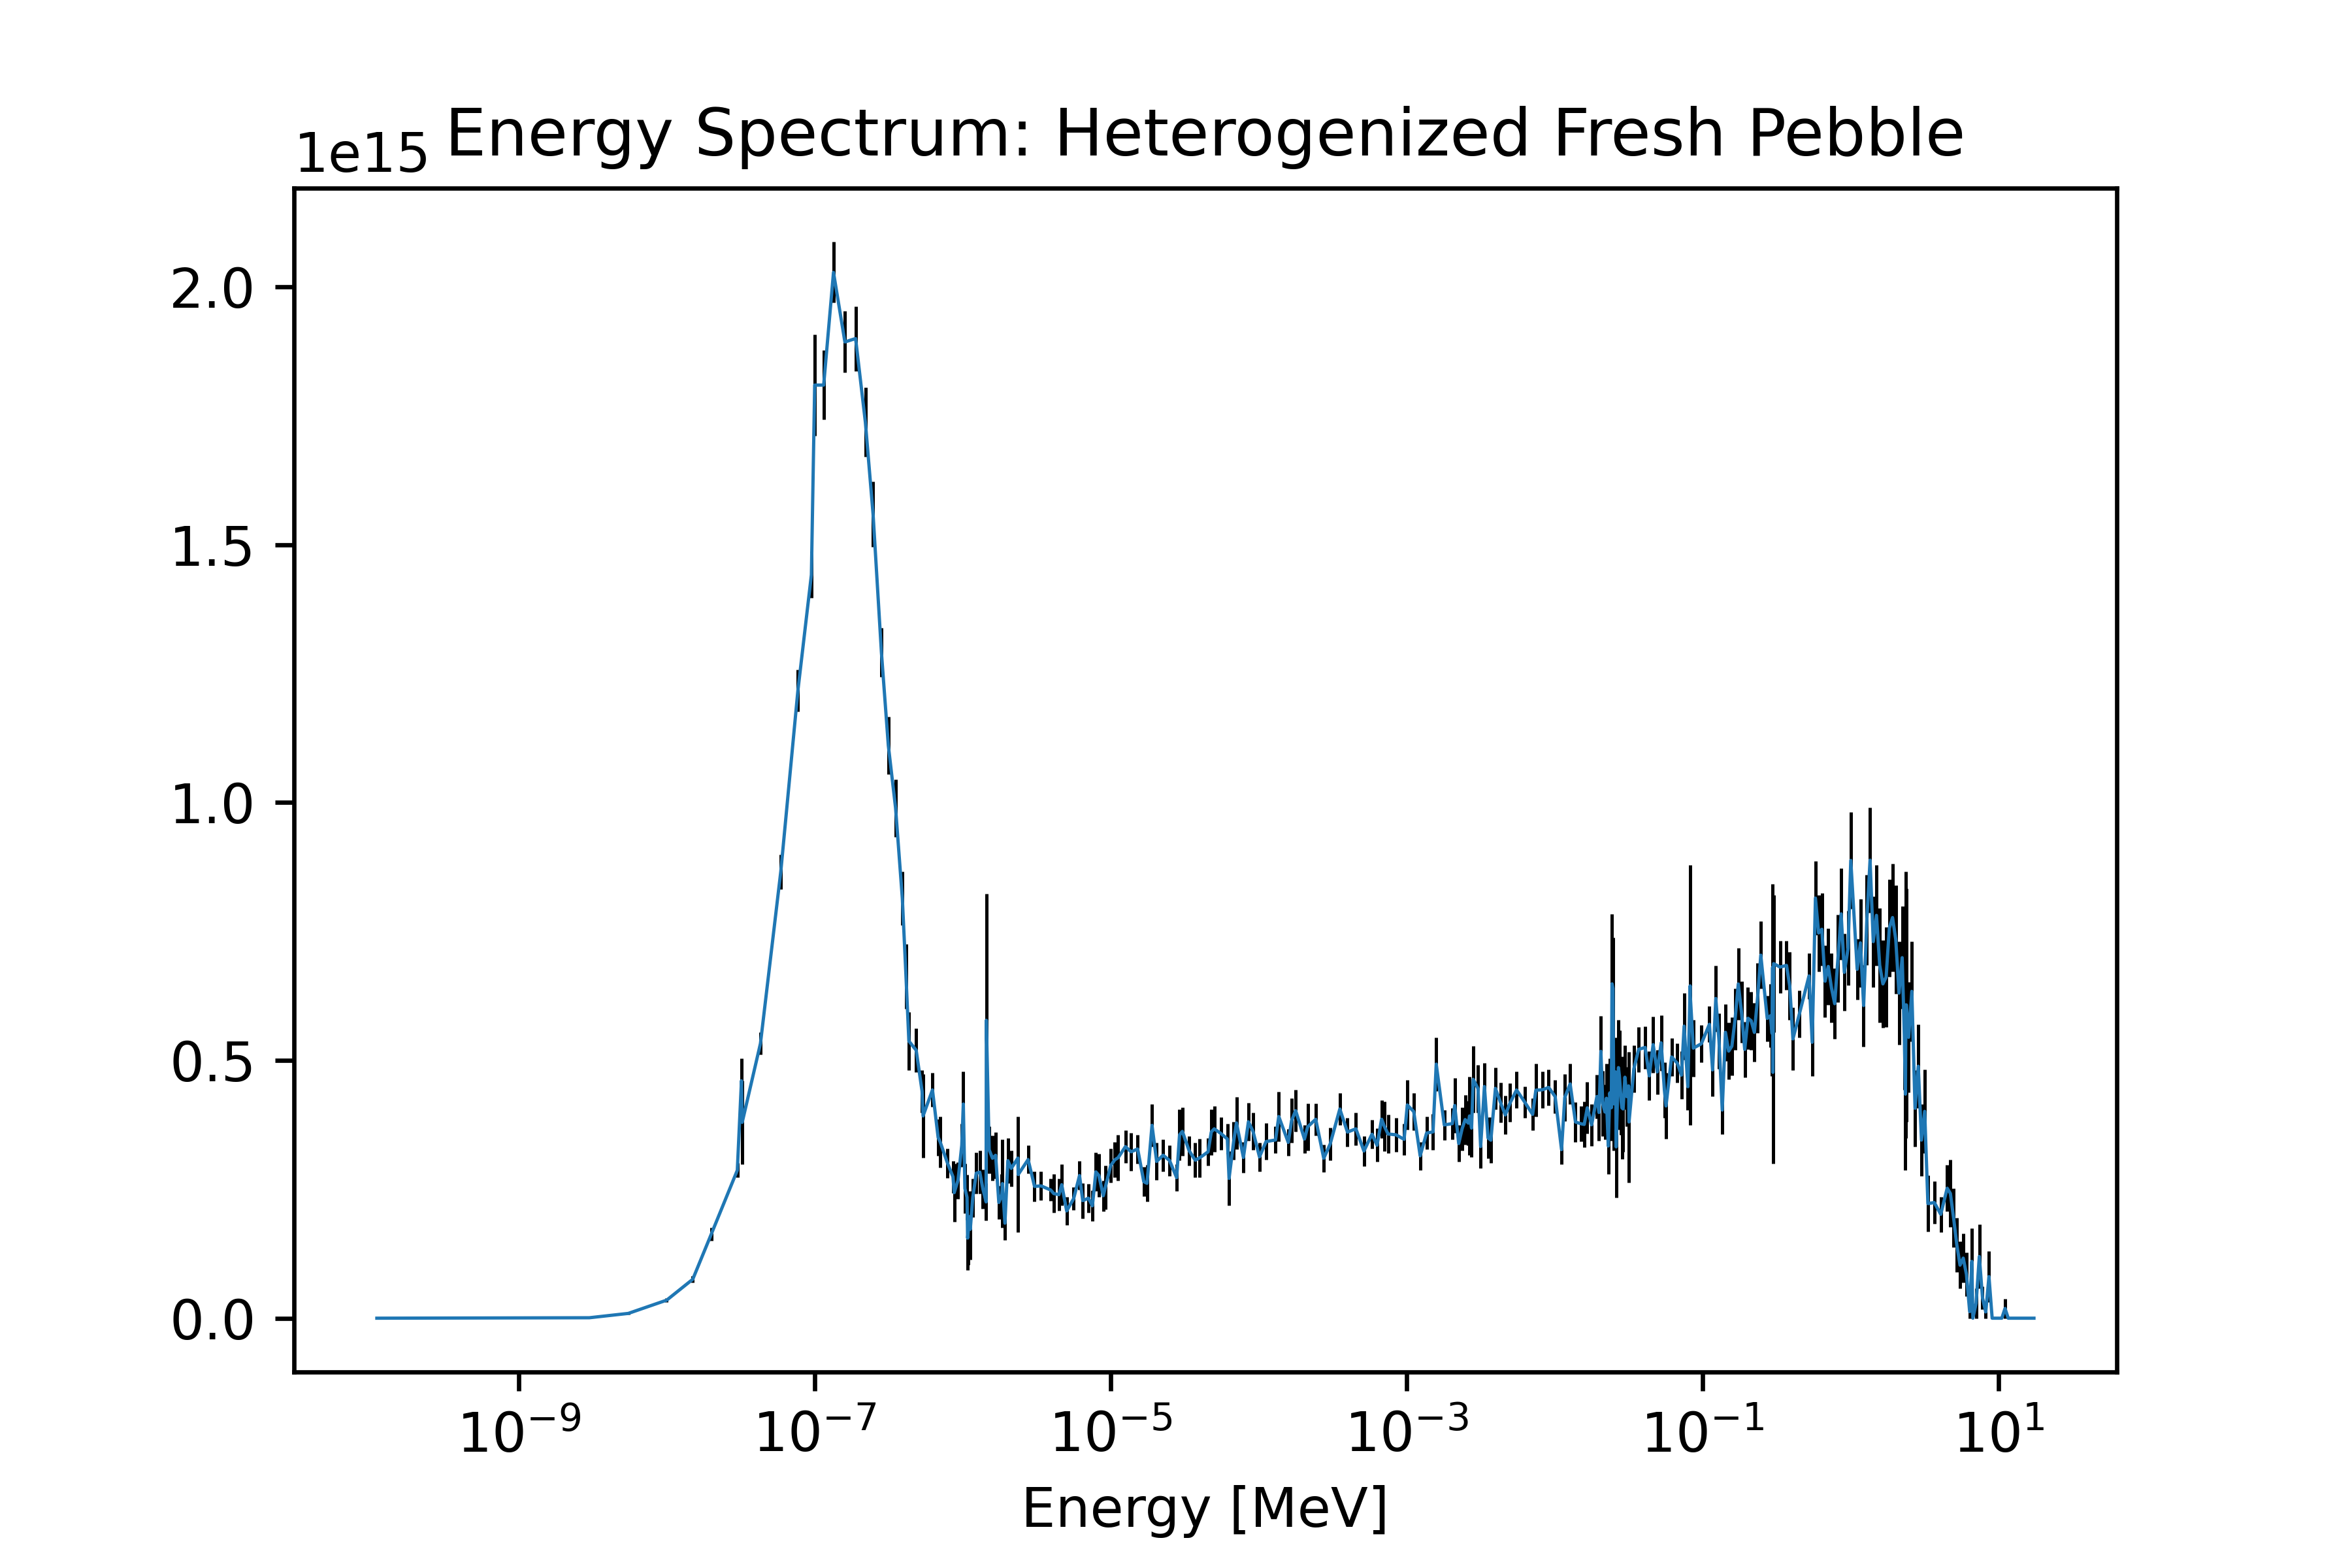
\includegraphics[width=0.95\linewidth]{figures/fresh_spec_het}
  \caption{Fresh Pebble Spectrum}
  \label{fig:het-fresh}
\end{subfigure}%


\begin{subfigure}{0.95\textwidth}
  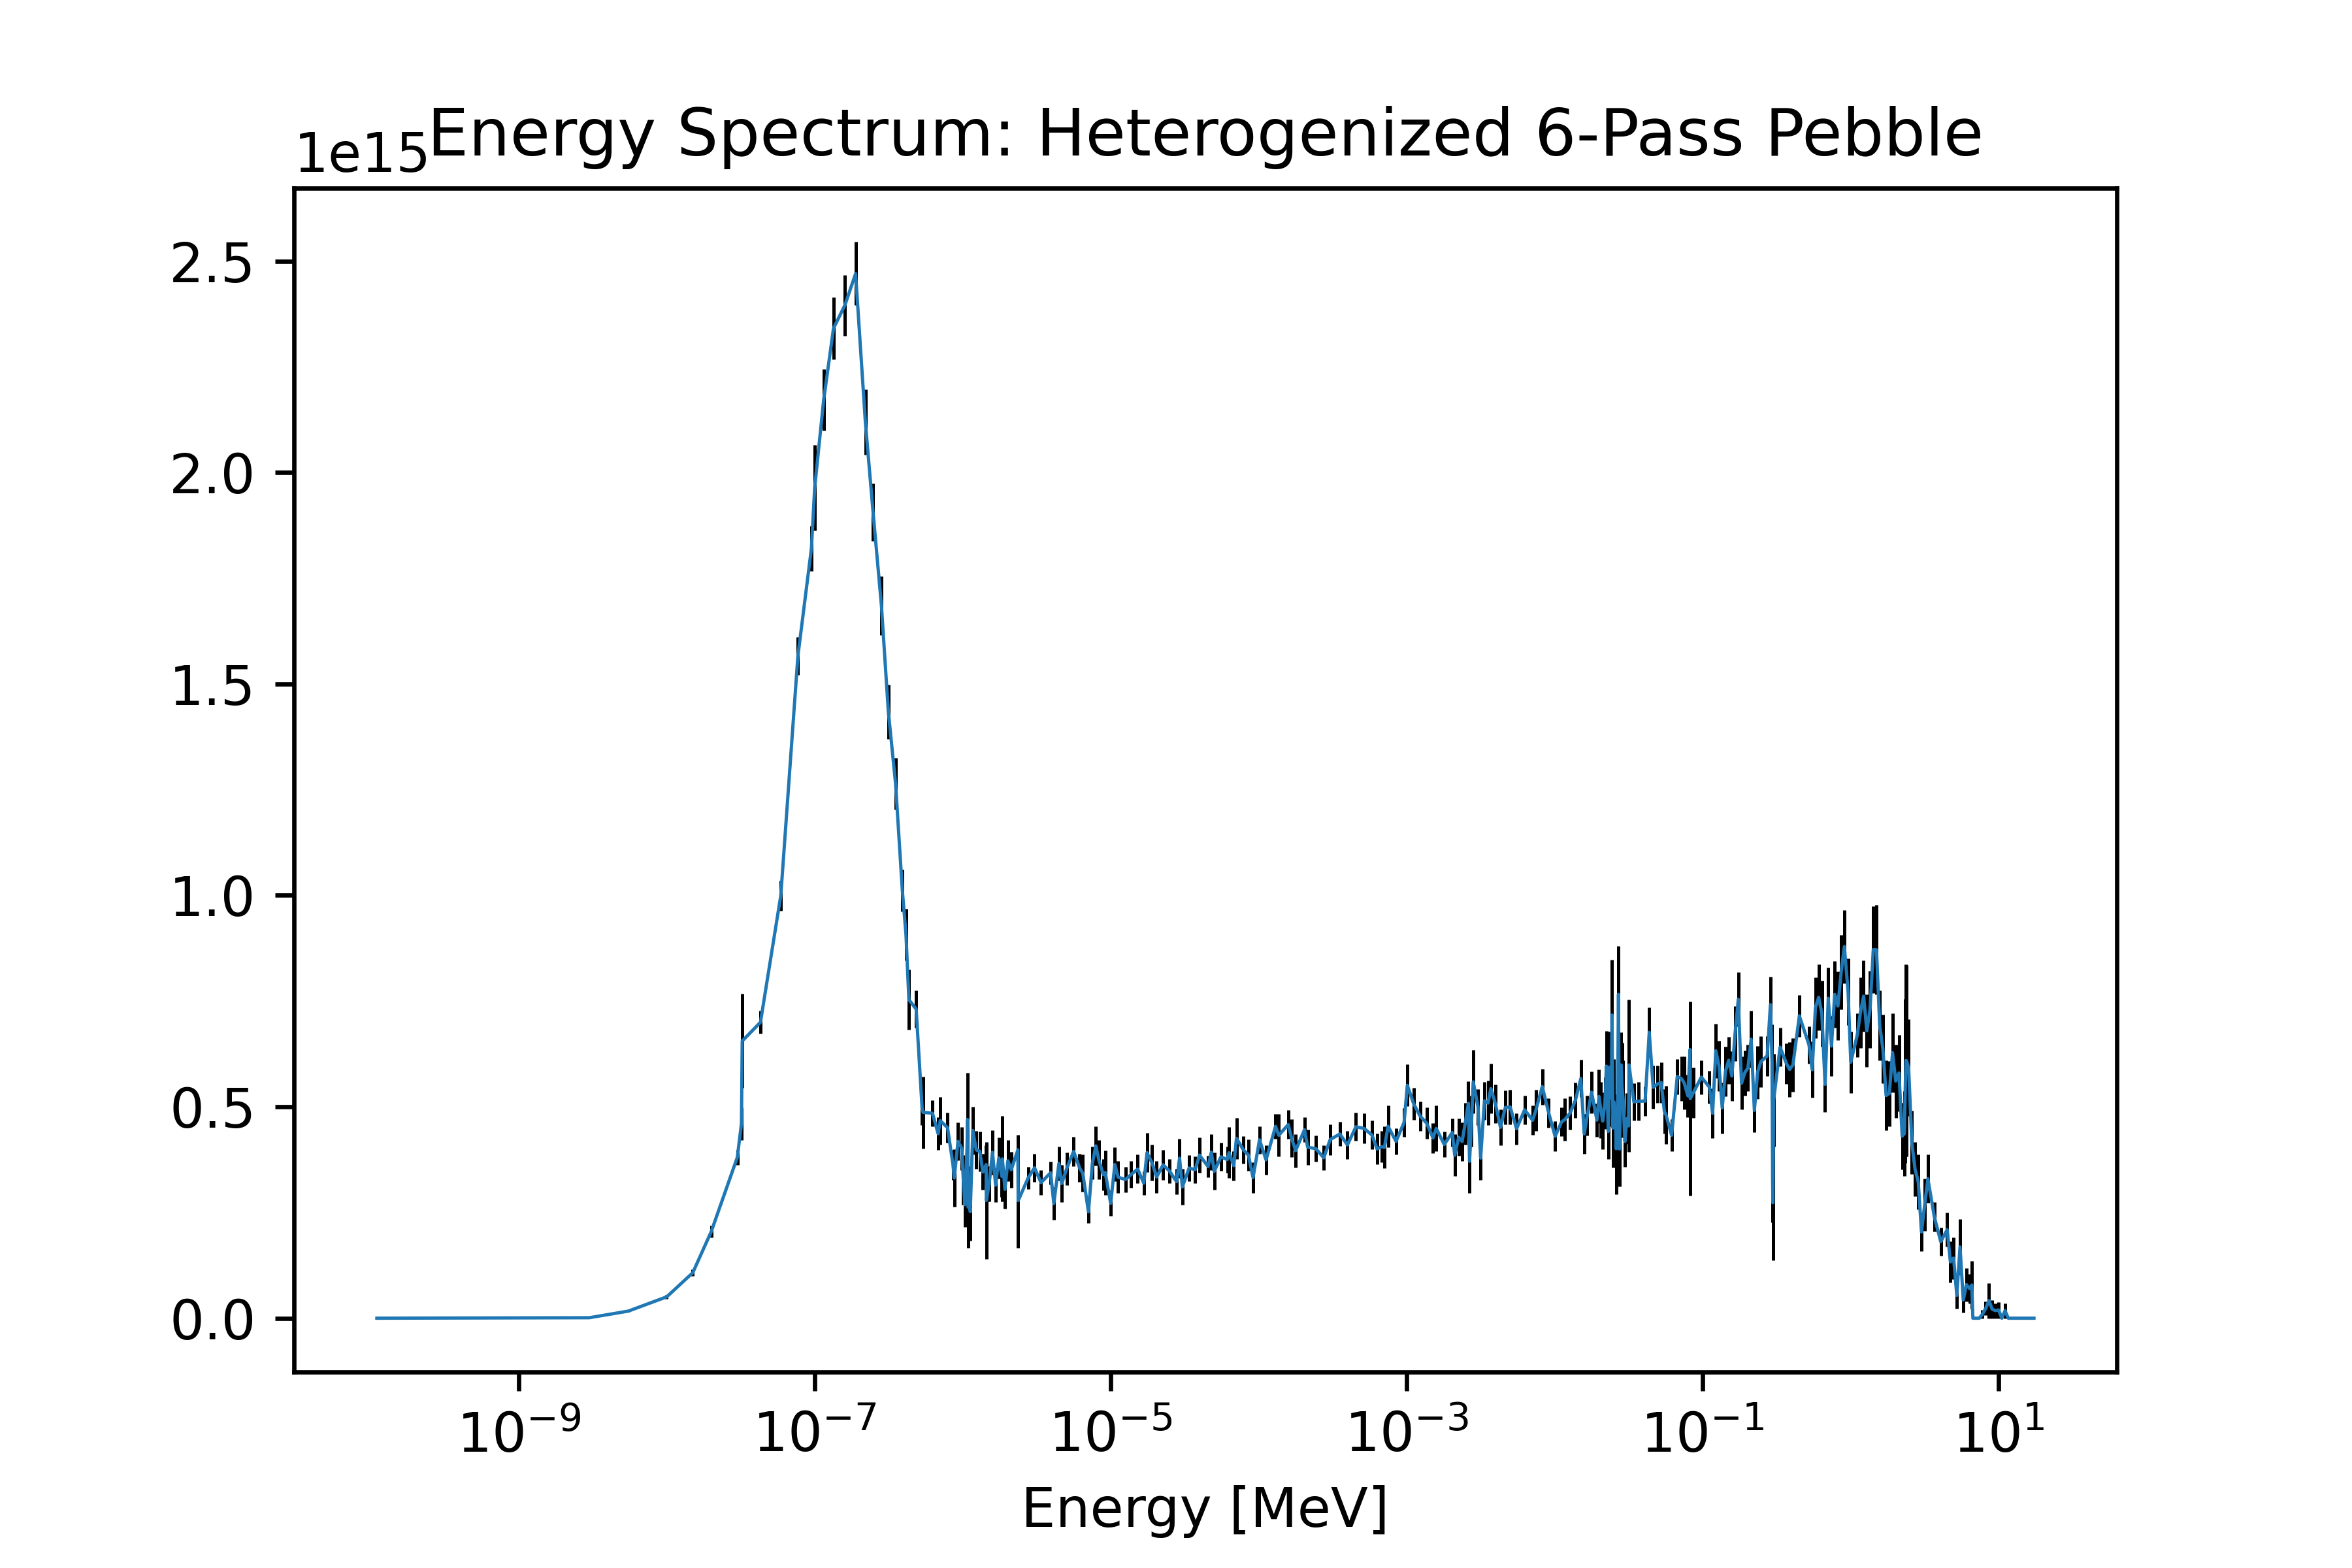
\includegraphics[width=0.95\linewidth]{figures/6_spec_het}
  \caption{Six-Pass Pebble Spectrum}
  \label{fig:het-six}
\end{subfigure}%

\caption{Lethargy Adjusted Neutron Flux Energy Spectra: Core Using Heterogenized Pebbles (cont.)}
\end{figure}

\begin{figure}[H]\ContinuedFloat
\centering

\begin{subfigure}{0.95\textwidth}
  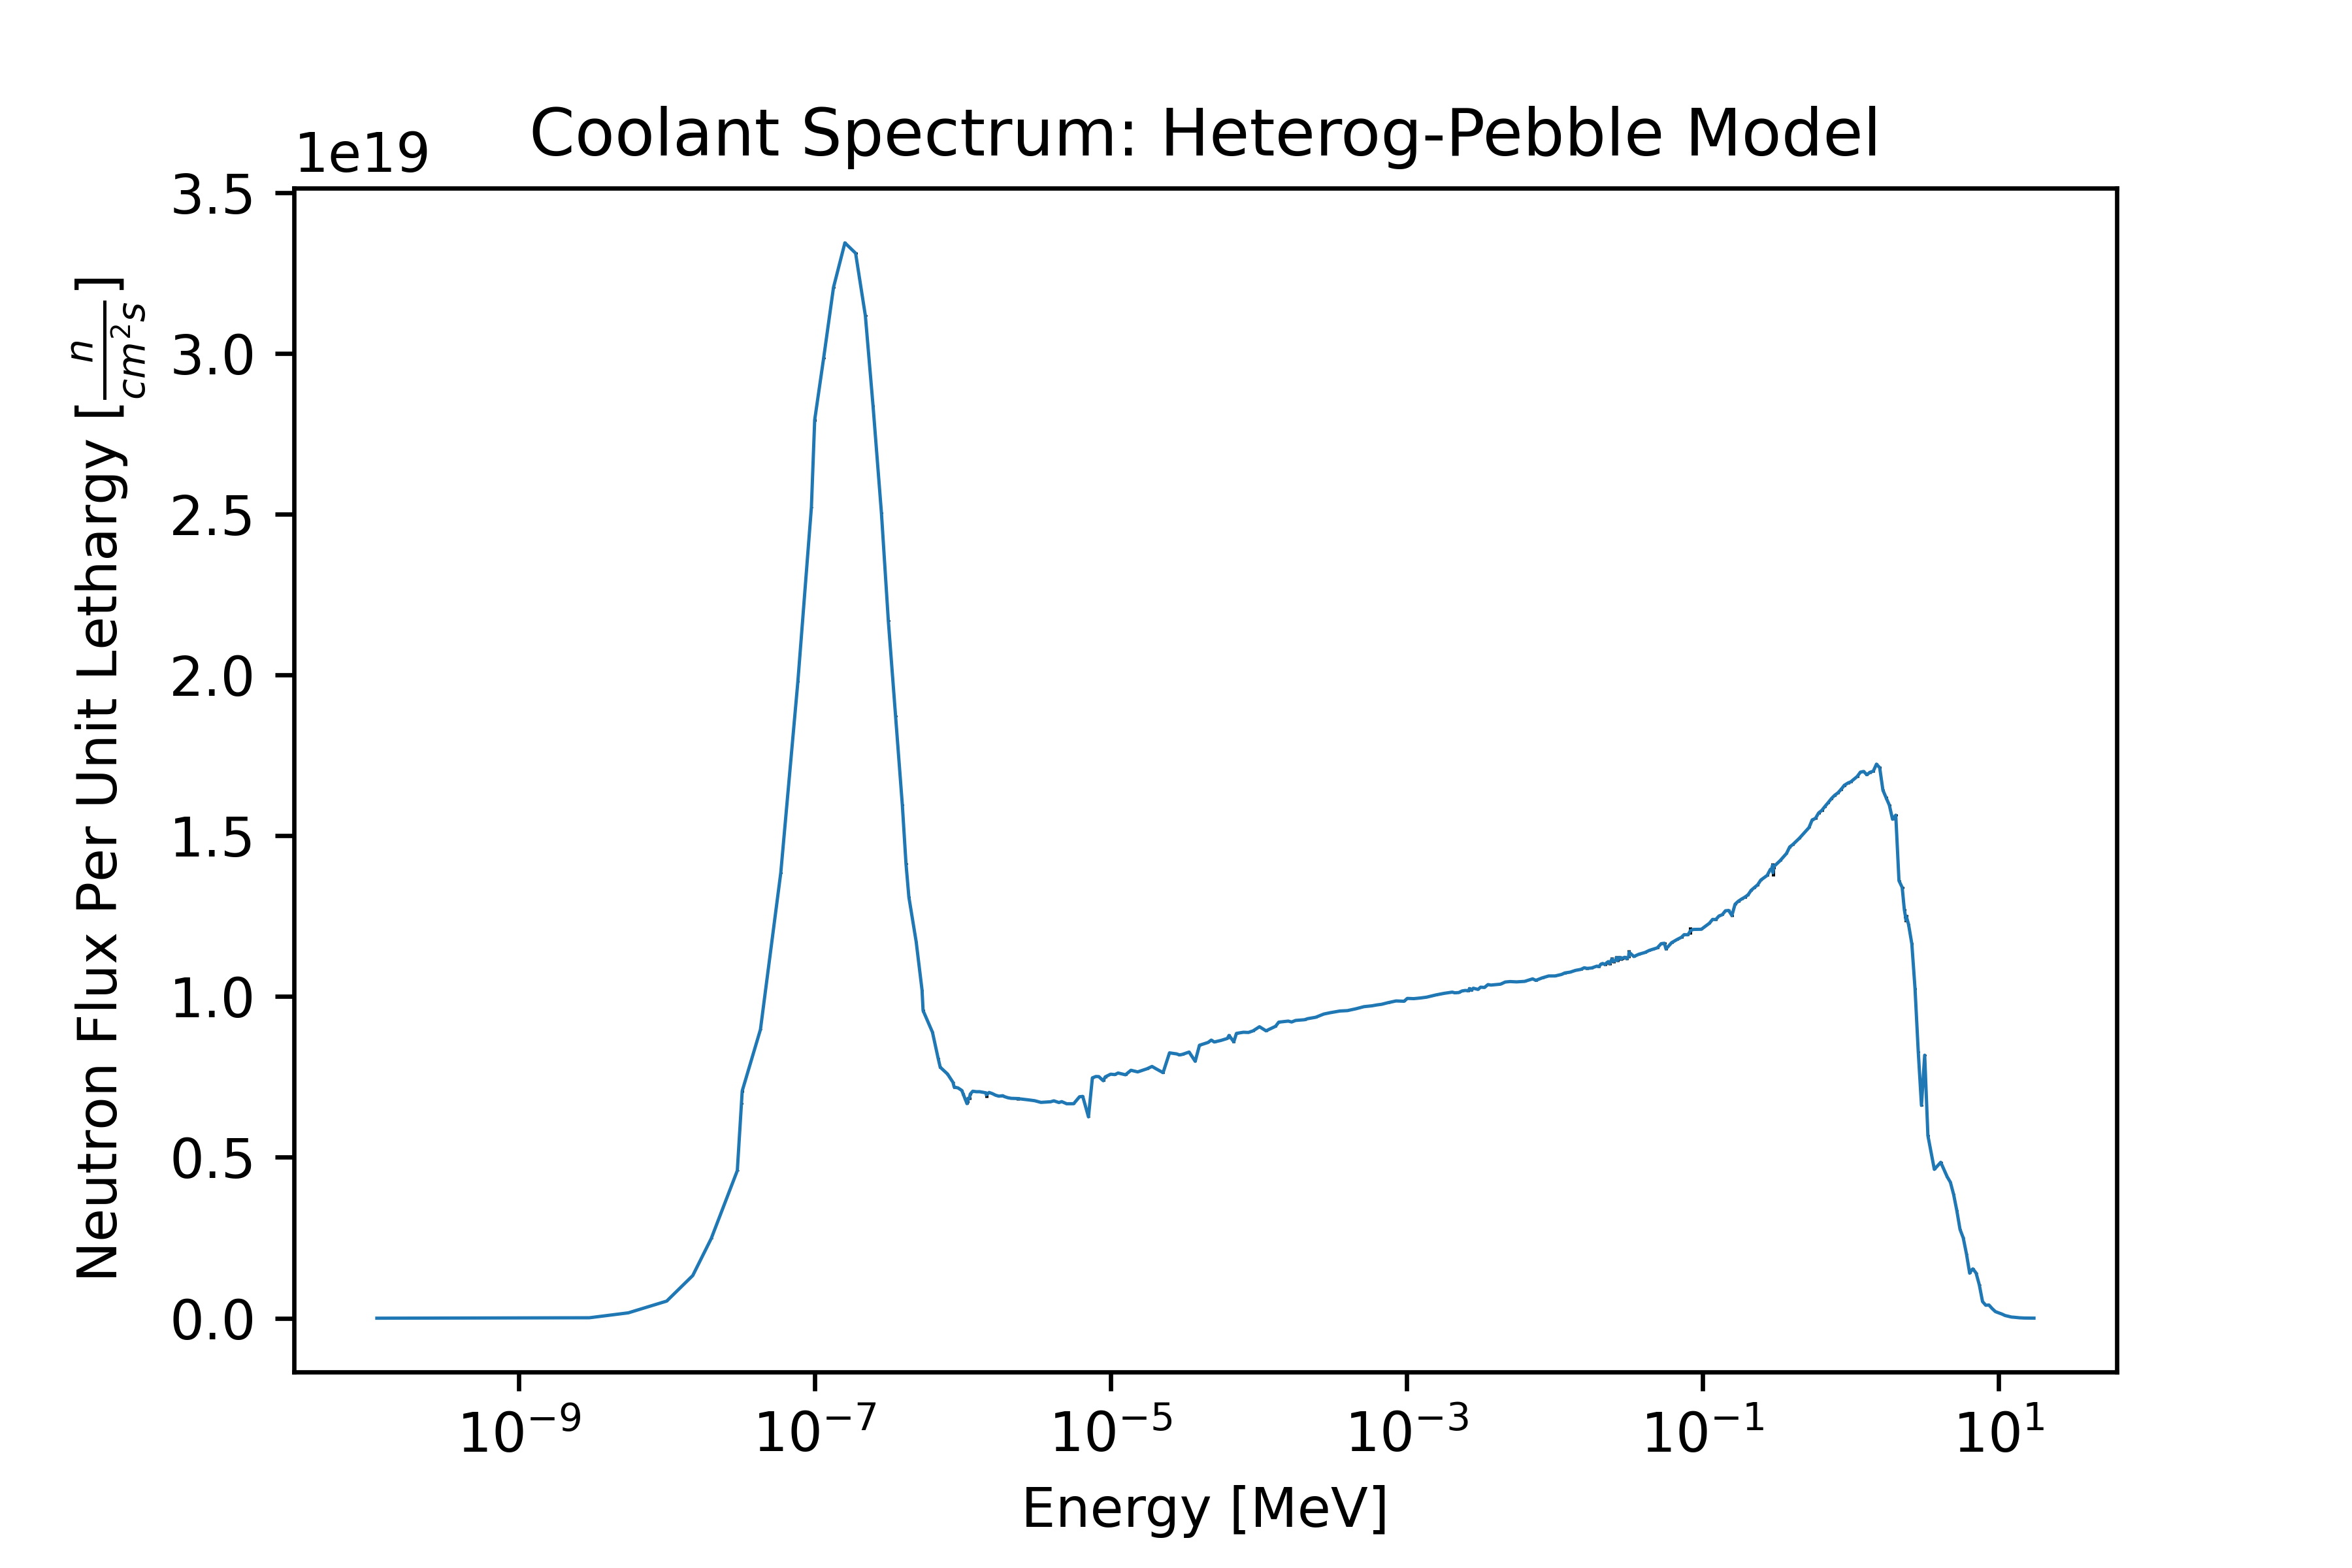
\includegraphics[width=0.95\linewidth]{figures/cool_spec_het}
  \caption{Coolant Spectrum}
  \label{fig:het-cool}
\end{subfigure}%


\begin{subfigure}{0.95\textwidth}
  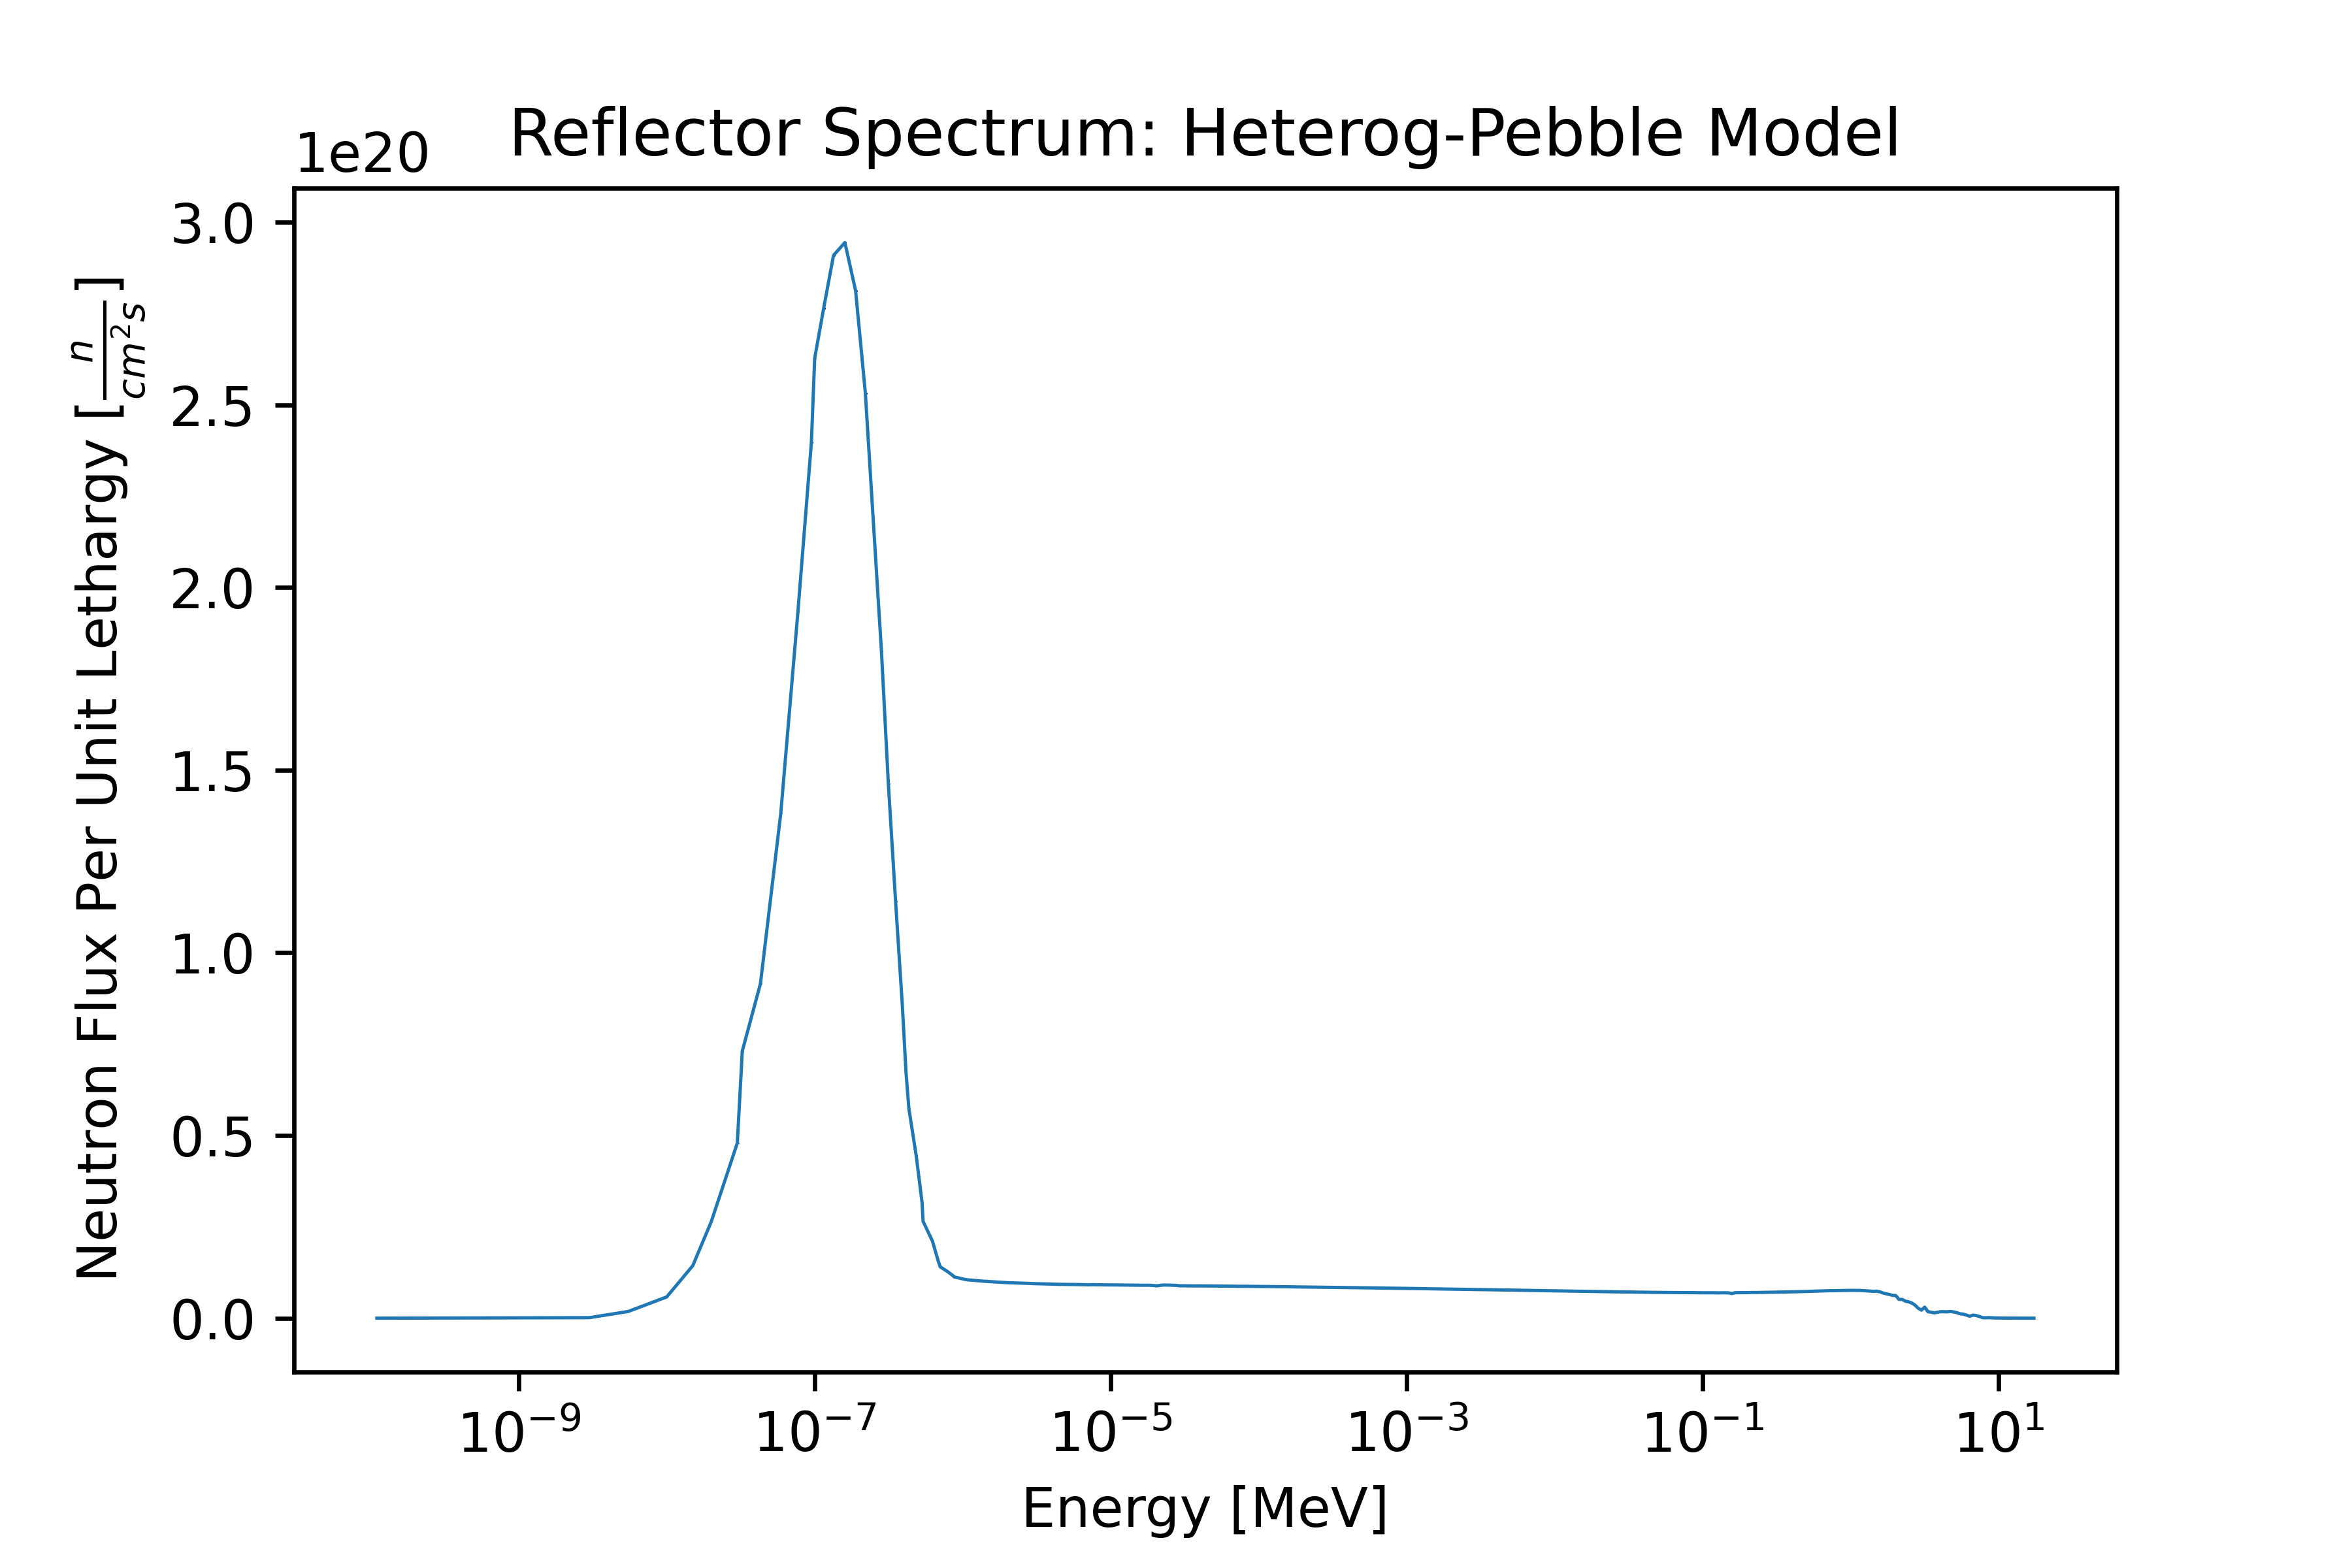
\includegraphics[width=0.95\linewidth]{figures/reflect_spec_het}
  \caption{Reflector Spectrum}
  \label{fig:het-reflec}
\end{subfigure}%


\caption{Lethargy Adjusted Neutron Flux Energy Spectra: Core Using Heterogenized Pebbles (cont.)}
\label{fig:hom-spec}
\end{figure}

The spectra for the Sangamon20 core using heterogenized TRISO particles are shown in Figures \ref{fig:het-core} through \ref{fig:het-cool}, much like the flux profiles, are of a similar morphology.  In order to better examine the differences between the homogenized and heterogenized versions, Figures \ref{fig:diff-flux} and \ref{fig:diff-spec} plot the simple relative difference for all spectra, and the radial fast and thermal profiles.  The relative difference calculation used the following:

\begin{align}
\Delta i &= \frac{i_{homogenized} - i_{heterogenized}}{i_{heterogenized}}
\intertext{where}
\Delta i&= \mbox{ relative difference for parameter i between homogenized and heterogenized model }\nonumber\\
i_{homogenized}&= \mbox{ homogenized parameter i}\nonumber\\
i_{heterogenized}&= \mbox{ heterogenized parameter i}\nonumber\\
\end{align}

And error calculation followed simple error propagation rules \cite{noauthor_uncertainties_nodate}.


\begin{figure}[H]
\centering

\begin{subfigure}{0.9\textwidth}
  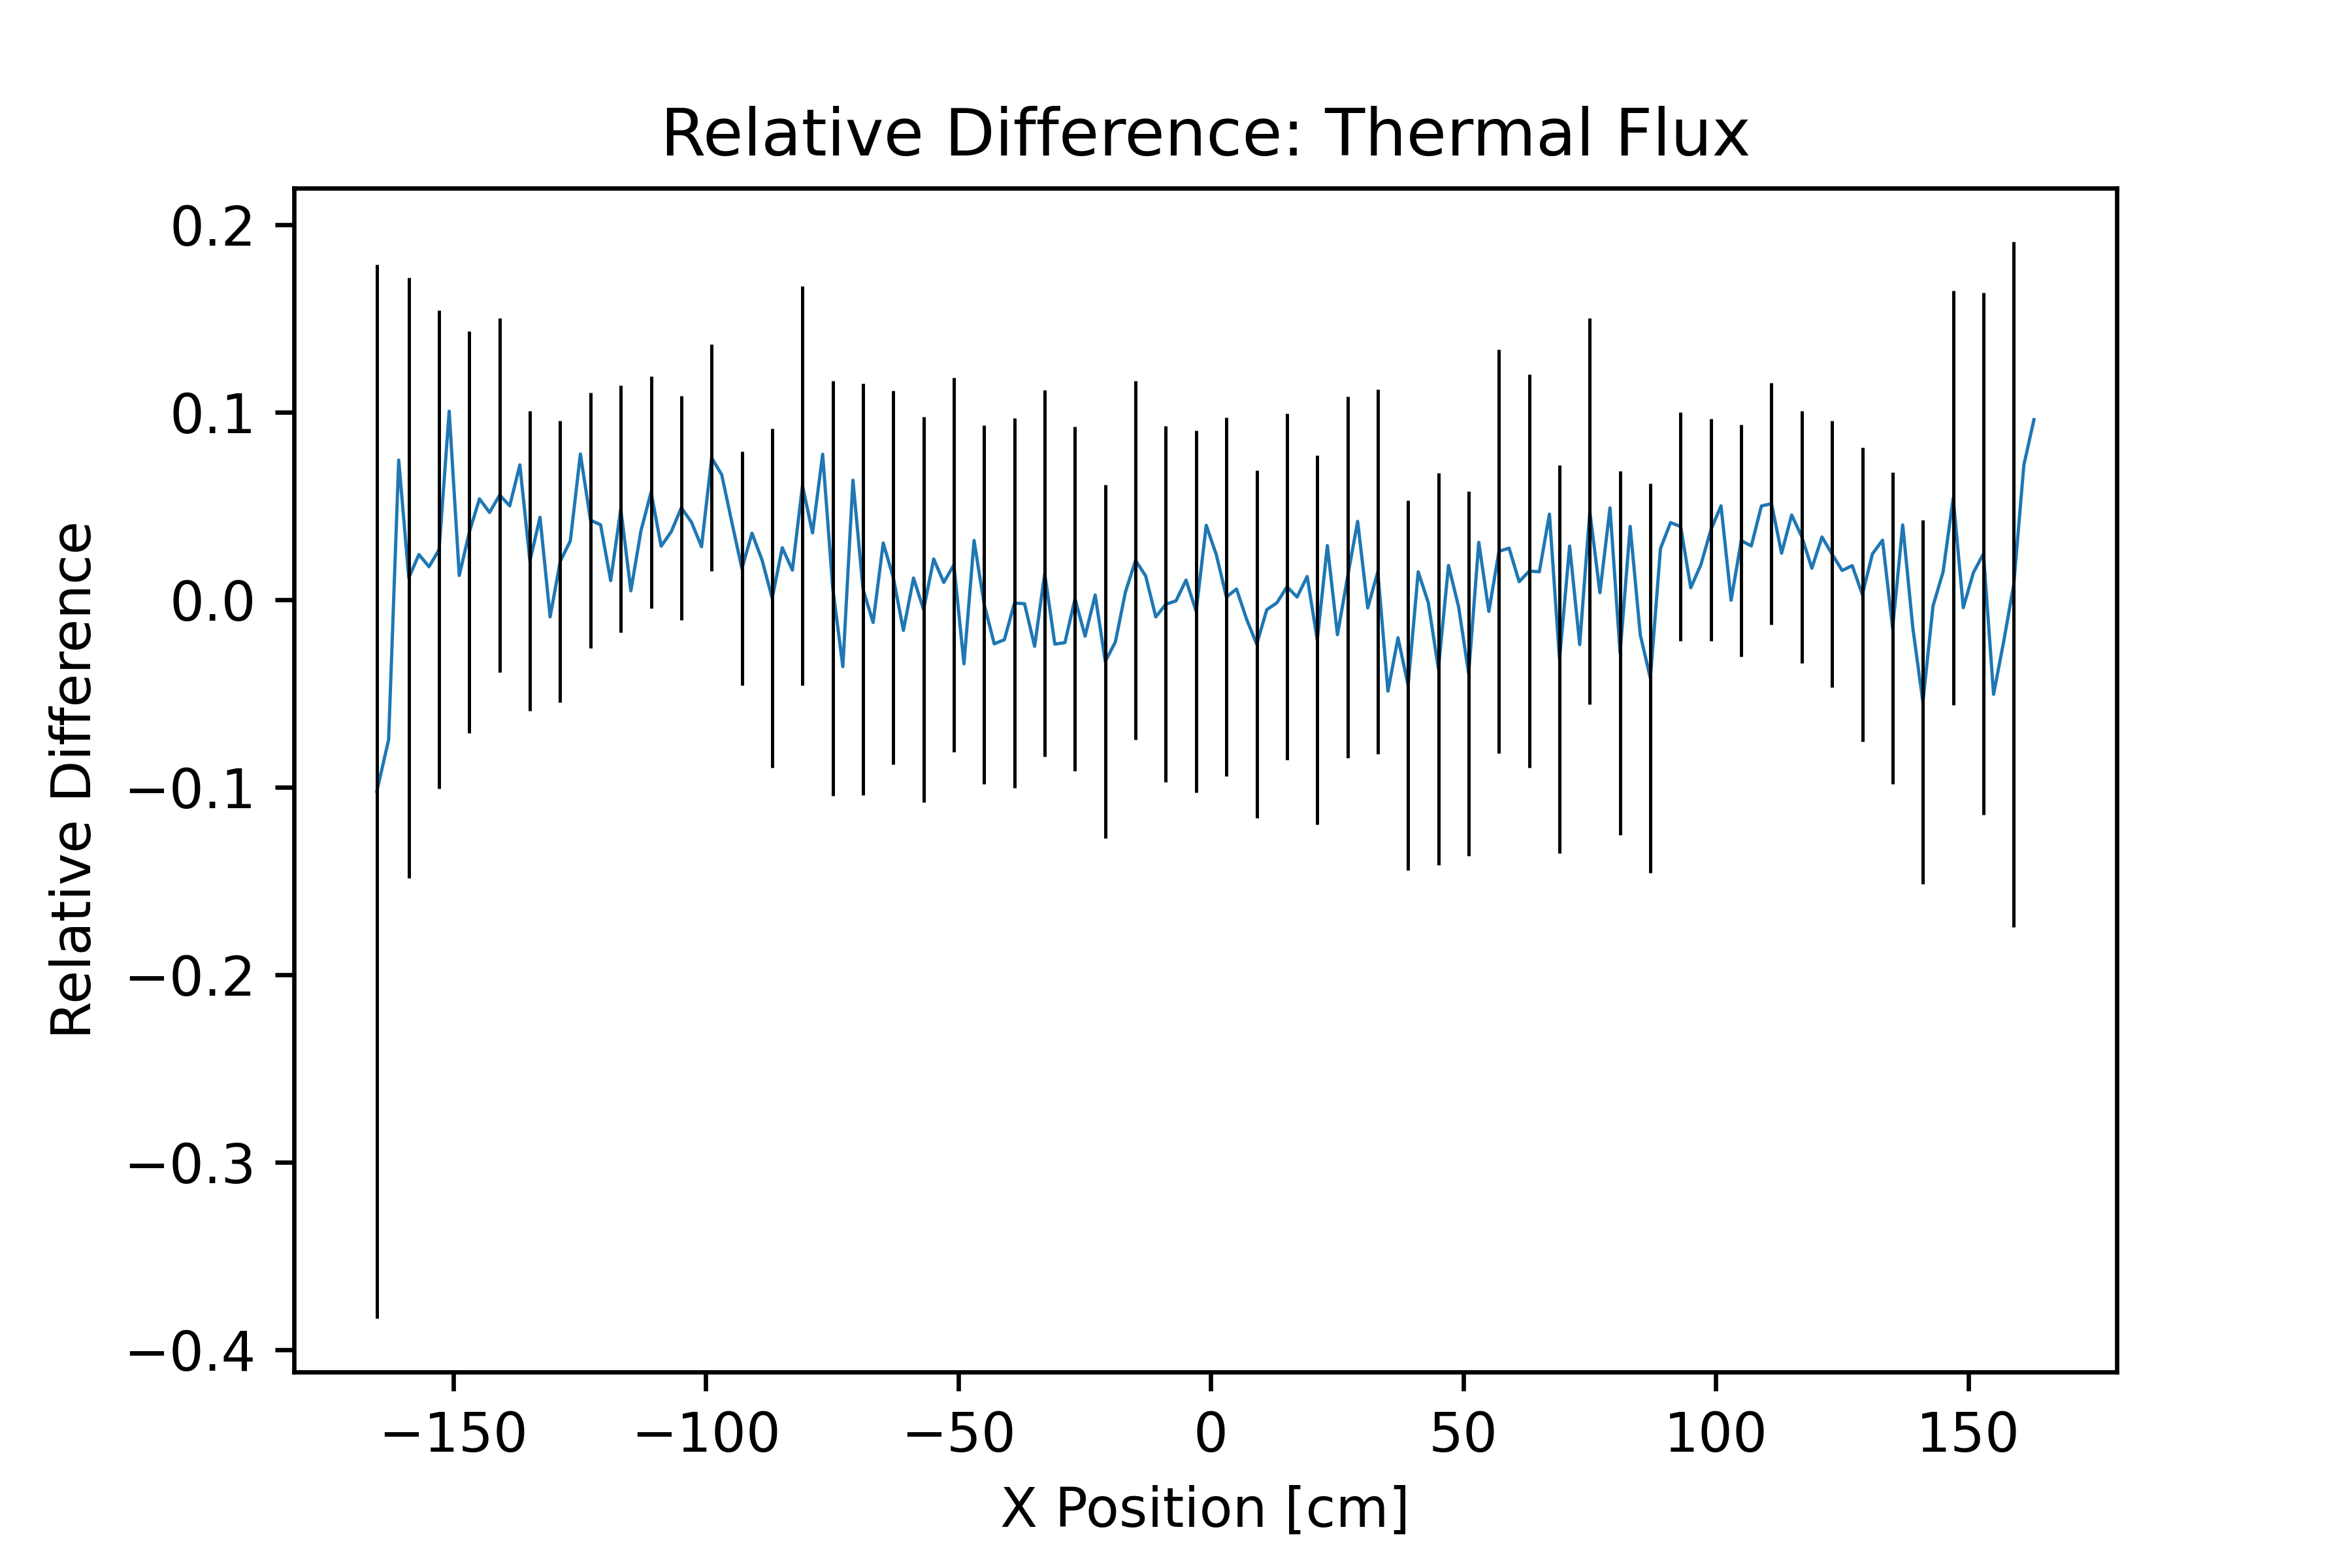
\includegraphics[width=0.9\linewidth]{figures/reldiff_therm_flux.png}
  \caption{Thermal Flux}
  \label{fig:diff-therm}
\end{subfigure}%

\caption{Relative Difference in Radial Thermal and Fast Flux Profiles Between Cores Using Homogenized and Heterogenized Pebbles}
\end{figure}

\begin{figure}[H]\ContinuedFloat
\centering

\begin{subfigure}{0.9\textwidth}
  \includegraphics[width=0.9\linewidth]{figures/reldiff_fast_flux.png}
  \caption{Fast Flux}
  \label{fig:diff-fast}
\end{subfigure}

%
\caption[]{(cont.)}
\label{fig:diff-flux}
\end{figure}

The relative difference in the thermal flux is generally between $\pm 10\%$ for the entire span of the reactor.  However, once one accounts for error, it is entirely possible that these differences are wholly accounted for with error alone.  The magnitude of the error is fairly constant --- except at the edges, where it is much larger.  For the fast flux spectrum, the active core region containing the fuel pebbles has a similarly low range of $\pm 10-20\%$ relative difference, which is once again accounted for by error.  The error on the outer edges in the fast flux plot is much greater than that in the thermal flux, but this is to be expected --- as said before, the reflector causes significant thermalization of neutrons entering it, and this means that there are fewer fast neutrons in the reflector to contribute to tallies.

For both the thermal and fast flux profiles, error only worsens on the outermost edges.  Overall, Figures \ref{fig:diff-therm} and \ref{fig:diff-fast} suggest that the homogenized simulation is slightly over-predicting the magnitude of the flux; however, given the size of the error, these differences do not exist with certainty.


\begin{figure}[H]
\centering
%
\begin{subfigure}{0.95\textwidth}
  \includegraphics[width=0.95\linewidth]{figures/reldiff_core_spec_er}
  \caption{Core}
  \label{fig:diff-core}
\end{subfigure}%


\begin{subfigure}{0.95\textwidth}
  \includegraphics[width=0.95\linewidth]{figures/reldiff_fresh_spec_er}
  \caption{Fresh Pebble}
  \label{fig:diff-fresh}
\end{subfigure}%

\caption{Relative Difference in Lethargy Adjusted Neutron Flux Energy Spectra Between Cores using Homogenized and Heterogenized Pebbles}
\end{figure}

\begin{figure}[H]\ContinuedFloat
\centering

\begin{subfigure}{0.95\textwidth}
  \includegraphics[width=0.95\linewidth]{figures/reldiff_six_spec_er}
  \caption{Six-Pass Pebble}
  \label{fig:diff-six}
\end{subfigure}%


\begin{subfigure}{0.95\textwidth}
  \includegraphics[width=0.95\linewidth]{figures/reldiff_cool_spec_er}
  \caption{Coolant}
  \label{fig:diff-cool}
\end{subfigure}%

\caption[]{(cont.)}
\end{figure}

\begin{figure}[H]\ContinuedFloat
\centering

\begin{subfigure}{0.95\textwidth}
  \includegraphics[width=0.95\linewidth]{figures/reldiff_reflec_spec_er}
  \caption{Reflector}
  \label{fig:diff-reflec}
\end{subfigure}%

\caption[]{(cont.)}
\label{fig:diff-spec}
\end{figure}

Overall, the homogenized model is over-predicting the thermal peak compared with heterogenized in the core spectra by 5\%.  Around $10\times10^{-06}$ MeV, just after the thermal peak, the two spectra agree before diverging again, this time with a slightly greater disagreement.  Unlike Figure \ref{fig:diff-flux}, error alone leaves the relative differences seen in Figure \ref{fig:diff-spec} unaccounted for (with the exception of the highest neutron energy ranges).

The coolant spectra differed after the thermal peak in a magnitude and shape matching the differences in core spectra.  Unlike the core, however, the coolant has much closer agreement at lower energy levels, including at the thermal peak.  The reflector shows a slight over estimation for the homogeneous spectra, which is consistent for all but the highest energy levels.

It is in the pebble spectra that we see the most dramatic disagreement.  Around the thermal peak, in both Figures \ref{fig:diff-fresh} and \ref{fig:diff-six} (note the change in y-axis scale compared to others in Figures \ref{fig:het-core}, \ref{fig:het-reflec}, and \ref{fig:het-cool}) , the relative difference spikes; though the error is still substantial in this region compared with the peaks in the relative difference.  Between $10\times10^{-07}$ and $5\times10^{-02}$, the differences are minimal and likely accounted for by noise or error.  Between $10\times10^{-02}$ and $10\times10^{-01}$, the difference has a slight blip, which may be indicative of a fission product with a resonance around this region.

The most dramatic peaks occur in the sixth-pass pebble at 0.2995 MeV, at which point the homogenized reactor is over-predicting the lethargy-adjusted neutron flux by a factor of 2.69.  Both the fresh and sixth-pass spectra have another peak at higher energy levels - fresh peaks at 6.3763 MeV, while the sixth-pass spectra has its second peak at 5.2205 MeV.  One possibility is that the $^{235}U$ in the pebble is more likely to undergo fission in a homogenized pebble, which disperses the $^{235}U$ atoms in what is almost pure graphite.



\section{Shuffling and Symmetry Tests}
Two additional studies look at the effects of assuming a one-sixth core symmetry, and the effects of changing the fuel composition in each pebble, effectively shuffling the pebbles without re-generating their location.  All tests use the homogenized pebble assumption as a base.

\subsection{Effects of Symmetry Assumption}
\label{res-sym}

Overall, the effects of using a one-sixth core symmetry were minimal.  For both Table \ref{table:slicesens} and Table \ref{table:shufsens}, the relative difference between $k_{eff}$ and $J^+$ are calculated between the value provided in the table, and the same parameter in the Sangamon20 control model (see \autoref{res-control}).



\begin{table}[H]
\centering
\caption{Symmetry Run Results Summary}
 \begin{tabularx}{0.7\textwidth}{c  c  c  c  c}
 	\hline
 	Run & $k_{eff}$ & $k_{eff}$ $\% \Delta$ & $J^+$  $[\frac{n}{cm^2s}]$ & $J^+$ $\% \Delta$  \\
 	\hline
 	Run 1 & 1.03990 $\pm$ 0.00055 & 0.0836$\%$ & $5.921\times10^{11}$ $\pm$ $8.704\times10^{08}$ & 0.626$\%$ \\
 	Run 2 & 1.03979 $\pm$ 0.00050 & 0.0942$\%$ & $5.884\times10^{11}$ $\pm$ $8.296\times10^{08}$ & 0.010$\%$ \\
 	Run 3 & 1.04150 $\pm$ 0.00054 & 0.0701$\%$ & $5.908\times10^{11}$ $\pm$ $7.444\times10^{08}$ & 0.392$\%$ \\
 	Run 4 & 1.03927 $\pm$ 0.00057 & 0.144$\%$ & $5.910\times10^{11}$ $\pm$ $8.687\times10^{08}$ & 0.425$\%$ \\
 	Run 5 & 1.04154 $\pm$ 0.00054 & 0.0740$\%$ & $5.884\times10^{11}$ $\pm$ $8.885\times10^{08}$ & 0.010$\%$ \\
 	Run 6 & 1.04047 $\pm$ 0.00050 & 0.0288$\%$ & $5.888\times10^{11}$ $\pm$ $8.478\times10^{08}$ & 0.057$\%$ \\
 	\hline

 \end{tabularx}
\label{table:slicesens}
\end{table}

Figure \ref{fig:0-60} provides cross-sections of the geometry, and fission rate/thermal flux meshes for the one-sixth core symmetry test.  The fission rate mesh naturally exhibits a six-part repeating pattern, and still shows the banding patterns on the outer edges. 


\begin{figure}[h!]
\centering

\begin{subfigure}{0.45\textwidth}
  \includegraphics[width=0.95\linewidth]{figures/0-60/0-60-r}
  \caption{Radial Cross Section at y=0}
  \label{fig:0-60-r}
\end{subfigure}%
%
\begin{subfigure}{0.45\textwidth}
  \includegraphics[width=0.95\linewidth]{figures/0-60/0-60-rm}
  \caption{Radial Mesh}
  \label{fig:0-60-rm}
\end{subfigure}

\begin{subfigure}{0.45\textwidth}
  \includegraphics[width=0.95\linewidth]{figures/0-60/0-60-v}
  \caption{Axial Cross Section at z=0 }
  \label{fig:0-60-v}
\end{subfigure}
%
\begin{subfigure}{0.45\textwidth}
  \includegraphics[width=0.95\linewidth]{figures/0-60/0-60-vm}
  \caption{Axial Mesh}
  \label{fig:0-60-vm}
\end{subfigure}
%
\caption{Sensitivity Analysis: $0^{\circ}$ - $60^{\circ}$}
\label{fig:0-60}
\end{figure}
One point of interest is the degree to which the region from 0 to 60 degrees matches the same region in the control fission rate mesh.  An image subtraction program generated Figure \ref{fig:htgr-diff} by subtracting the radial meshes for the control (Figure \ref{fig:controlb}) and first symmetry test (Figure \ref{fig:0-60-rm}).

\begin{figure}[h!]
\centering
\includegraphics[width=0.6\linewidth]{figures/htgr-diff}
\caption{An Image Generated by Subtracting \ref{fig:0-60-rm} from \ref{fig:htgr-diff}.}
\label{fig:htgr-diff}
\end{figure}

Within the region between 0 and 60 degrees, the two meshes are almost identical, pixel for pixel.  While this might be unsurprising in the center of this region, the perfect match towards the edges of it are less so.  As a reminder, the symmetry tests all use a one-sixth symmetry, and a periodic boundary condition, i.e., if a neutron leaves the slice on one side, it re-enters the slice on the other.  In effect, the edges of the 0 to 60 degree slice in the symmetry test are seeing entirely different materials, compared with the control.  The edges in \ref{fig:htgr-diff} are not a gradient, but rather a hard line, which may suggest that with proper mixing nearest-neighbor pebbles have a relatively lesser impact on core parameters.  However, note that Sangamon20 uses only fuel pebbles, and this observation may be false in a reactor design using, for example, absorber pebbles containing something such as boron, or inert pebbles at the edge to protect the reflector.  For the full results of all symmetry tests, see \autoref{app-sym}.


\subsection{Effects of Pebble Shuffling}
\label{res-shuff}

The final test on the effects of changes to core modeling is another test of consistency between similar HTGR designs with a different pebble configurations.  Rather than re-generate the pebble locations several times, the 'shuffling' test simply reassigns each pebble with a different fuel composition (creating a new input file).  For example, the pebbles that were once fresh are now first-pass, the first pass pebbles are now second-pass, and so on.  The manual shuffling followed the process outlined in \autoref{meth-sens}, Table \ref{table:shuffle}, and the results of this test are in Table \ref{table:shufsens}.



\begin{table}[H]
\centering
 \begin{tabularx}{0.7\textwidth}{c  c  c  c  c}
 	\hline
 	Run & $k_{eff}$ & $k_{eff}$ $\% \Delta$ & $J^+$  $[\frac{n}{cm^2s}]$ & $J^+$ $\% \Delta$ \\
 	\hline
 	Run 1 & 1.03994 $\pm$ 0.00054 & 0.0797$\%$ & $5.897\times10^{11}$ $\pm$ $8.668\times10^{08}$ & 0.211$\%$ \\
 	Run 2 & 1.03999 $\pm$ 0.00055 & 0.0749$\%$ & $5.902\times10^{11}$ $\pm$ $8.086\times10^{08}$  & 0.295$\%$ \\
 	Run 3 & 1.04002 $\pm$ 0.00053 & 0.0721$\%$ & $5.896\times10^{11}$ $\pm$ $8.490\times10^{08}$ & 0.192$\%$  \\
 	Run 4 & 1.04103 $\pm$ 0.00057 & 0.0249$\%$ & $5.884\times10^{11}$ $\pm$ $9.355\times10^{08}$ & 0.013$\%$ \\
 	Run 5 & 1.03960 $\pm$ 0.00053 & 0.112$\%$ & $5.904\times10^{11}$ $\pm$ $8.443\times10^{08}$ & 0.329$\%$  \\
 	Run 6 & 1.04014 $\pm$ 0.00057 & 0.0605$\%$ & $5.898\times10^{11}$ $\pm$ $7.726\times10^{08}$ & 0.227$\%$ \\
 	\hline

 \end{tabularx}
\caption{Shuffling Run Summary}
\label{table:shufsens}
\end{table}

Overall, much like the symmetry test, re-mixing the pebbles had little effect on overall results.  Likely, provided the pebbles are sufficiently mixed, and no 'pockets' of like pebbles exist, designs that are otherwise identical should provide similar results.  For all geometry cross-sections and thermal flux/fission rate mesh images, and the results of image difference for each run, see \autoref{app-shuf}.

\chapter{Conclusion}
\section{Summary and Discussion}

Previous work in HTGR pebble-bed modeling noticed that the specific lattice arrangement used, by-and-large, did not significantly affect results.  The pebble-shuffling test combined with the symmetry test support this observation in regards to a completely random arrangement of pebbles.

The symmetry test showed that for minimal banding - areas of same pebbles creating streaks and rings once reflected - the difference between a full core model and one using symmetry to simplify is minimal.  Additionally, for models which assume a well-mixed core, the differences between otherwise-identical models with a different dispersal of pebbles are minimal.  For other models, this suggests that one does not need to re-create the same reactor over and over with slightly different pebble arrangements in order to accurately characterize a core.

The heterogenized tests highlight the need for an accurate representation of TRISO particles.  While the overall differences between the flux profiles are minimal, the homogenized pebbles will under-predict k-eff by more than 4.0\%, while over-predicting the magnitude of the neutron energy lethargy-adjusted flux spectra by as much as 5.0\%.  The most significant change is in the spectra within the pebbles themselves, where high-energy neutron peaks are over-estimated in the fresh and six-pass pebbles by a factor of 2-4.  Additionally, the outer current, which was used to gauge the effectiveness of the reflector, did not significantly change between the two models, likely because the reflector is unchanged between the two versions, and the reflector is thick enough to thermalize the fast neutrons entering from the core before they reach the outer edge, so changes in the fast neutron population in the active core don't have a noticeable effect on the outermost reaches.

For isotopic inventories, most isotopes either increased or decreased at a uniform rate with each pass through the core.  However, some isotopes, such as Pu-239, reach a peak concentration in MOL, and subsequently decline.  The isotopes that increase over pebble lifetime versus decrease is a point of consideration when choosing between multipass and OTTO fuel cycles.


\section{Future Work}

The symmetry test showed that, with random mixing, simplifying the model by approximating the whole-core with only a slice of it had minimal effects for a $\frac{1}{6}$ and greater symmetry.  However, the 'banding' and petal-like pebble patterns this symmetry created highlights a potential issue, however unlikely.  What if the random pebble dispersal happens to lump a large number of same or similar burnup pebbles together?  How would this affect a whole core model?  What of a model using symmetry?  Future work could explore the effects of pebble 'lumping', such as the size of pebble-lump needed before an effect is seen in the core model.

Additionally, this reactor model used an infinite lattice of like pebbles in the depletion model to arrive at an equilibrium composition.  While this is a fine first-guess, it is possible to improve the accuracy of the equilibrium composition.  For example, one could track compositions over time in the actual core, as opposed to an infinite lattice, or split the core into axial layers, and track the pebble isotopic inventory not simply as a function of the number of passes, but passes and current height in the core.

The current model is not thermodynamically optimal, and future work could adjust the height-diameter ratio, provided it follows \ref{fig-rh-vol.tex}.  Given that there is a slight excess reactivity, there should be room to shift to a slightly less critical shape that is more thermally beneficial.  If there is still a slight excess reactivity at this point, one could explore adding in an additional "half-pass" - i.e., half of the six-pass pebbles go for a seventh pass, and the other half are removed and replaced with fresh pebbles.  Alternatively, one could explore the addition of absorber pebbles to handle excess reactivity.

Finally, the pebble dispersal method used here does not account for gravity, which would make the pebbles settle a bit closer together.  Without shaking the core (not recommended, it would almost certainly make the issue of pebble dust worse, if not crack pebbles entirely) or using a core that has a diameter which is an integer multiple of the pebble diameter, it is not possible to get a perfect close-pack arrangement.  One could simulate the effects of gravity by dispersing the pebbles not over the whole volume, but rather a volume with a slightly shorter height.  However, it is important to note that at a packing fraction of around 0.58, the model is already approaching the theoretical maximum packing fraction, so the difference this would make may be minimal.

\backmatter
\nocite{*}
\bibliographystyle{apa}
\bibliography{bibliography}

\mainmatterWithoutReset
\appendix
\chapter{}
Appendix.

\section{Appendix A: Symmetry Test}

\begin{figure}[h!]
\centering

\begin{subfigure}{0.45\textwidth}
  \includegraphics[width=0.95\linewidth]{figures/60-120/60-120-r}
  \caption{Radial Cross Section at y=0}
  \label{fig:bstep0}
\end{subfigure}%
%
\begin{subfigure}{0.45\textwidth}
  \includegraphics[width=0.95\linewidth]{figures/60-120/60-120-rm}
  \caption{Radial Mesh}
  \label{fig:bstep1}
\end{subfigure}

\begin{subfigure}{0.45\textwidth}
  \includegraphics[width=0.95\linewidth]{figures/60-120/60-120-v}
  \caption{Axial Cross Section at z=0 }
  \label{fig:bstep1}
\end{subfigure}
%
\begin{subfigure}{0.45\textwidth}
  \includegraphics[width=0.95\linewidth]{figures/60-120/60-120-vm}
  \caption{Axial Mesh}
  \label{fig:bstep1}
\end{subfigure}
%
\caption{Sensitivity Analysis: $60^{\circ}$ - $120^{\circ}$}
\label{fig:60-120}
\end{figure}
\begin{figure}[H]
\centering
\includegraphics[width=0.6\linewidth]{figures/60-120/diff-60-120}
\caption{An Image Generated by Subtracting Figure \ref{fig:60-120-rm} from Figure \ref{fig:controlb}.}
\label{fig:60-120-diff}
\end{figure}

\begin{figure}[H]
\centering

\begin{subfigure}{0.45\textwidth}
  \includegraphics[width=0.95\linewidth]{figures/120-180/120-180-r}
  \caption{Radial Cross Section at y=0}
  \label{fig:120-180-r}
\end{subfigure}%
%
\begin{subfigure}{0.45\textwidth}
  \includegraphics[width=0.95\linewidth]{figures/120-180/120-180-rm}
  \caption{Radial Mesh}
  \label{fig:120-180-rm}
\end{subfigure}

\begin{subfigure}{0.45\textwidth}
  \includegraphics[width=0.95\linewidth]{figures/120-180/120-180-v}
  \caption{Axial Cross Section at z=0 }
  \label{fig:120-180-v}
\end{subfigure}
%
\begin{subfigure}{0.45\textwidth}
  \includegraphics[width=0.95\linewidth]{figures/120-180/120-180-vm}
  \caption{Axial Mesh}
  \label{fig:120-180-vm}
\end{subfigure}
%
\caption{Sensitivity Analysis: $120^{\circ}$ - $180^{\circ}$}
\label{fig:120-180}
\end{figure}
\begin{figure}[H]
\centering
\includegraphics[width=0.6\linewidth]{figures/120-180/diff-120-180}
\caption{An Image Generated by Subtracting \ref{fig:120-180-rm} from \ref{fig:controlb}.}
\label{fig:120-180-diff}
\end{figure}


\begin{figure}
\centering

\begin{subfigure}{0.45\textwidth}
  \includegraphics[width=0.95\linewidth]{figures/180-240/180-240-r}
  \caption{Radial Cross Section at y=0}
  \label{fig:bstep0}
\end{subfigure}%
%
\begin{subfigure}{0.45\textwidth}
  \includegraphics[width=0.95\linewidth]{figures/180-240/180-240-rm}
  \caption{Radial Mesh}
  \label{fig:bstep1}
\end{subfigure}

\begin{subfigure}{0.45\textwidth}
  \includegraphics[width=0.95\linewidth]{figures/180-240/180-240-v}
  \caption{Axial Cross Section at z=0 }
  \label{fig:bstep1}
\end{subfigure}
%
\begin{subfigure}{0.45\textwidth}
  \includegraphics[width=0.95\linewidth]{figures/180-240/180-240-vm}
  \caption{Axial Mesh}
  \label{fig:bstep1}
\end{subfigure}
%
\caption{Sensitivity Analysis: $180^{\circ}$ - $240^{\circ}$}
\label{fig:180-240}
\end{figure}
\begin{figure}[H]
\centering
\includegraphics[width=0.6\linewidth]{figures/180-240/diff-180-240}
\caption{An Image Generated by Subtracting Figure \ref{fig:180-240-rm} from Figure \ref{fig:controlb}.}
\label{fig:180-240-diff}
\end{figure}


\begin{figure}
\centering

\begin{subfigure}{0.45\textwidth}
  \includegraphics[width=0.95\linewidth]{figures/240-300/240-300-r}
  \caption{Radial Cross Section at y=0}
  \label{fig:bstep0}
\end{subfigure}%
%
\begin{subfigure}{0.45\textwidth}
  \includegraphics[width=0.95\linewidth]{figures/240-300/240-300-rm}
  \caption{Radial Mesh}
  \label{fig:bstep1}
\end{subfigure}

\begin{subfigure}{0.45\textwidth}
  \includegraphics[width=0.95\linewidth]{figures/240-300/240-300-v}
  \caption{Axial Cross Section at z=0 }
  \label{fig:bstep1}
\end{subfigure}
%
\begin{subfigure}{0.45\textwidth}
  \includegraphics[width=0.95\linewidth]{figures/240-300/240-300-vm}
  \caption{Axial Mesh}
  \label{fig:bstep1}
\end{subfigure}
%
\caption{Sensitivity Analysis: $240^{\circ}$ - $300^{\circ}$}
\label{fig:240-300}
\end{figure}
\begin{figure}[H]
\centering
\includegraphics[width=0.6\linewidth]{figures/240-300/diff-240-300}
\caption{An Image Generated by Subtracting Figure \ref{fig:240-300-rm} from Figure \ref{fig:controlb}.}
\label{fig:240-300-diff}
\end{figure}


\begin{figure}[H]
\centering

\begin{subfigure}{0.45\textwidth}
  \includegraphics[width=0.95\linewidth]{figures/300-360/300-360-r}
  \caption{Radial Cross Section at y=0}
  \label{fig:bstep0}
\end{subfigure}%
%
\begin{subfigure}{0.45\textwidth}
  \includegraphics[width=0.95\linewidth]{figures/300-360/300-360-rm}
  \caption{Radial Mesh}
  \label{fig:bstep1}
\end{subfigure}

\begin{subfigure}{0.45\textwidth}
  \includegraphics[width=0.95\linewidth]{figures/300-360/300-360-v}
  \caption{Axial Cross Section at z=0 }
  \label{fig:bstep1}
\end{subfigure}
%
\begin{subfigure}{0.45\textwidth}
  \includegraphics[width=0.95\linewidth]{figures/300-360/300-360-vm}
  \caption{Axial Mesh}
  \label{fig:bstep1}
\end{subfigure}
%
\caption{Sensitivity Analysis: $300^{\circ}$ - $360^{\circ}$}
\label{fig:300-360}
\end{figure}
\begin{figure}[H]
\centering
\includegraphics[width=0.6\linewidth]{figures/300-360/diff-300-360}
\caption{An Image Generated by Subtracting \ref{fig:300-360-rm} from \ref{fig:controlb}.}
\label{fig:300-360-diff}
\end{figure}

\section{Appendix B: Shuffle Test}

\begin{figure}[H]
\centering

\begin{subfigure}{0.45\textwidth}
  \includegraphics[width=0.95\linewidth]{figures/1234560/1234560-r}
  \caption{Radial Cross Section at y=0}
  \label{fig:1234560-r}
\end{subfigure}%
%
\begin{subfigure}{0.45\textwidth}
  \includegraphics[width=0.95\linewidth]{figures/1234560/1234560-rm}
  \caption{Radial Mesh}
  \label{fig:1234560-rm}
\end{subfigure}

\begin{subfigure}{0.45\textwidth}
  \includegraphics[width=0.95\linewidth]{figures/1234560/1234560-v}
  \caption{Axial Cross Section at z=0 }
  \label{fig:1234560-v}
\end{subfigure}
%
\begin{subfigure}{0.45\textwidth}
  \includegraphics[width=0.95\linewidth]{figures/1234560/1234560-vm}
  \caption{Axial Mesh}
  \label{fig:1234560-vm}
\end{subfigure}
%
\caption{Shuffle Analysis: Run 1}
\label{fig:1234560}
\end{figure}
\begin{figure}[H]
\centering
\includegraphics[width=0.6\linewidth]{figures/shuffle/diff-1234560}
\caption{An Image Generated by Subtracting \ref{fig:diff-1234560-rm} from \ref{fig:controlb}.}
\label{fig:diff-1234560}
\end{figure}

\begin{figure}[H]
\centering

\begin{subfigure}{0.45\textwidth}
  \includegraphics[width=0.95\linewidth]{figures/2345601/2345601-r}
  \caption{Radial Cross Section at y=0}
  \label{fig:2345601-r}
\end{subfigure}%
%
\begin{subfigure}{0.45\textwidth}
  \includegraphics[width=0.95\linewidth]{figures/2345601/2345601-rm}
  \caption{Radial Mesh}
  \label{fig:2345601-rm}
\end{subfigure}

\begin{subfigure}{0.45\textwidth}
  \includegraphics[width=0.95\linewidth]{figures/2345601/2345601-v}
  \caption{Axial Cross Section at z=0 }
  \label{fig:2345601-v}
\end{subfigure}
%
\begin{subfigure}{0.45\textwidth}
  \includegraphics[width=0.95\linewidth]{figures/2345601/2345601-vm}
  \caption{Axial Mesh}
  \label{fig:2345601-vm}
\end{subfigure}
%
\caption{Shuffle Analysis: Run 2}
\label{fig:0-60}
\end{figure}
\begin{figure}[H]
\centering
\includegraphics[width=0.6\linewidth]{figures/shuffle/diff-2345601}
\caption{An Image Generated by Subtracting \ref{fig:2345601-rm} from \ref{fig:controlb}.}
\label{fig:diff-2345601}
\end{figure}

\begin{figure}[H]
\centering

\begin{subfigure}{0.45\textwidth}
  \includegraphics[width=0.95\linewidth]{figures/3456012/3456012-r}
  \caption{Radial Cross Section at y=0}
  \label{fig:3456012-r}
\end{subfigure}%
%
\begin{subfigure}{0.45\textwidth}
  \includegraphics[width=0.95\linewidth]{figures/3456012/3456012-rm}
  \caption{Radial Mesh}
  \label{fig:3456012-rm}
\end{subfigure}

\begin{subfigure}{0.45\textwidth}
  \includegraphics[width=0.95\linewidth]{figures/3456012/3456012-v}
  \caption{Axial Cross Section at z=0 }
  \label{fig:3456012-v}
\end{subfigure}
%
\begin{subfigure}{0.45\textwidth}
  \includegraphics[width=0.95\linewidth]{figures/3456012/3456012-vm}
  \caption{Axial Mesh}
  \label{fig:3456012-vm}
\end{subfigure}
%
\caption{Shuffle Analysis: Run 3}
\label{fig:3456012}
\end{figure}
\begin{figure}[H]
\centering
\includegraphics[width=0.6\linewidth]{figures/shuffle/diff-3456012}
\caption{An Image Generated by Subtracting Figure \ref{fig:3456012-rm} from Figure \ref{fig:controlb}.}
\label{fig:diff-3456012}
\end{figure}

\begin{figure}[H]
\centering

\begin{subfigure}{0.45\textwidth}
  \includegraphics[width=0.95\linewidth]{figures/4560123/4560123-r}
  \caption{Radial Cross Section at y=0}
  \label{fig:4560123-r}
\end{subfigure}%
%
\begin{subfigure}{0.45\textwidth}
  \includegraphics[width=0.95\linewidth]{figures/4560123/4560123-rm}
  \caption{Radial Mesh}
  \label{fig:4560123-rm}
\end{subfigure}

\begin{subfigure}{0.45\textwidth}
  \includegraphics[width=0.95\linewidth]{figures/4560123/4560123-v}
  \caption{Axial Cross Section at z=0 }
  \label{fig:4560123-v}
\end{subfigure}
%
\begin{subfigure}{0.45\textwidth}
  \includegraphics[width=0.95\linewidth]{figures/4560123/4560123-vm}
  \caption{Axial Mesh}
  \label{fig:4560123-vm}
\end{subfigure}
%
\caption{Shuffle Analysis: Run 4}
\label{fig:4560123}
\end{figure}
\begin{figure}[H]
\centering
\includegraphics[width=0.6\linewidth]{figures/shuffle/diff-4560123}
\caption{An Image Generated by Subtracting \ref{fig:4560123-rm} from \ref{fig:controlb}.}
\label{fig:diff-4560123}
\end{figure}

\begin{figure}[H]
\centering

\begin{subfigure}{0.45\textwidth}
  \includegraphics[width=0.95\linewidth]{figures/5601234/5601234-r}
  \caption{Radial Cross Section at y=0}
  \label{fig:5601234-r}
\end{subfigure}%
%
\begin{subfigure}{0.45\textwidth}
  \includegraphics[width=0.95\linewidth]{figures/5601234/5601234-rm}
  \caption{Radial Mesh}
  \label{fig:5601234-rm}
\end{subfigure}

\begin{subfigure}{0.45\textwidth}
  \includegraphics[width=0.95\linewidth]{figures/5601234/5601234-v}
  \caption{Axial Cross Section at z=0 }
  \label{fig:5601234-v}
\end{subfigure}
%
\begin{subfigure}{0.45\textwidth}
  \includegraphics[width=0.95\linewidth]{figures/5601234/5601234-vm}
  \caption{Axial Mesh}
  \label{fig:5601234-vm}
\end{subfigure}
%
\caption{Shuffle Analysis: Run 5}
\label{fig:5601234}
\end{figure}
\begin{figure}[H]
\centering
\includegraphics[width=0.6\linewidth]{figures/shuffle/diff-5601234}
\caption{An Image Generated by Subtracting \ref{fig:diff-5601234-rm} from \ref{fig:controlb}.}
\label{fig:diff-5601234}
\end{figure}

\begin{figure}[H]
\centering

\begin{subfigure}{0.45\textwidth}
  \includegraphics[width=0.95\linewidth]{figures/6012345/6012345-r}
  \caption{Radial Cross Section at y=0}
  \label{fig:6012345-r}
\end{subfigure}%
%
\begin{subfigure}{0.45\textwidth}
  \includegraphics[width=0.95\linewidth]{figures/6012345/6012345-rm}
  \caption{Radial Mesh}
  \label{fig:6012345-rm}
\end{subfigure}

\begin{subfigure}{0.45\textwidth}
  \includegraphics[width=0.95\linewidth]{figures/6012345/6012345-v}
  \caption{Axial Cross Section at z=0 }
  \label{fig:6012345-v}
\end{subfigure}
%
\begin{subfigure}{0.45\textwidth}
  \includegraphics[width=0.95\linewidth]{figures/6012345/6012345-vm}
  \caption{Axial Mesh}
  \label{fig:6012345-vm}
\end{subfigure}
%
\caption{Shuffle Analysis: Run 6}
\label{fig:6012345}
\end{figure}
\begin{figure}[H]
\centering
\includegraphics[width=0.6\linewidth]{figures/shuffle/diff-6012345}
\caption{An Image Generated by Subtracting Figure \ref{fig:6012345-rm} from Figure \ref{fig:controlb}.}
\label{fig:diff-6012345}
\end{figure}

\chapter{}
\section{Shuffle Test}
\label{app-shuf}
Appendix B contains the geometry cross sections, fission rate/thermal flux meshes, and image difference results from the shuffling tests (see \autoref{meth-sens}, Table \ref{table:shuffle}), which were omitted from the main report for brevity.


\begin{figure}[H]
\centering

\begin{subfigure}{0.45\textwidth}
  \includegraphics[width=0.95\linewidth]{figures/1234560/1234560-r}
  \caption{Radial Cross Section at y=0}
  \label{fig:1234560-r}
\end{subfigure}%
%
\begin{subfigure}{0.45\textwidth}
  \includegraphics[width=0.95\linewidth]{figures/1234560/1234560-rm}
  \caption{Radial Mesh}
  \label{fig:1234560-rm}
\end{subfigure}

\begin{subfigure}{0.45\textwidth}
  \includegraphics[width=0.95\linewidth]{figures/1234560/1234560-v}
  \caption{Axial Cross Section at z=0 }
  \label{fig:1234560-v}
\end{subfigure}
%
\begin{subfigure}{0.45\textwidth}
  \includegraphics[width=0.95\linewidth]{figures/1234560/1234560-vm}
  \caption{Axial Mesh}
  \label{fig:1234560-vm}
\end{subfigure}
%
\caption{Shuffle Analysis: Run 1}
\label{fig:1234560}
\end{figure}
\begin{figure}[H]
\centering
\includegraphics[width=0.6\linewidth]{figures/shuffle/diff-1234560}
\caption{An Image Generated by Subtracting \ref{fig:diff-1234560-rm} from \ref{fig:controlb}.}
\label{fig:diff-1234560}
\end{figure}

Figure \ref{fig:1234560} provides the thermal flux and fission rate meshes and geometric cross sections axially and radially.  Figure \ref{fig:diff-1234560} is the result of the image difference between the full core control mesh and Figure \ref{fig:1234560-rm}.

\begin{figure}[H]
\centering

\begin{subfigure}{0.45\textwidth}
  \includegraphics[width=0.95\linewidth]{figures/2345601/2345601-r}
  \caption{Radial Cross Section at y=0}
  \label{fig:2345601-r}
\end{subfigure}%
%
\begin{subfigure}{0.45\textwidth}
  \includegraphics[width=0.95\linewidth]{figures/2345601/2345601-rm}
  \caption{Radial Mesh}
  \label{fig:2345601-rm}
\end{subfigure}

\begin{subfigure}{0.45\textwidth}
  \includegraphics[width=0.95\linewidth]{figures/2345601/2345601-v}
  \caption{Axial Cross Section at z=0 }
  \label{fig:2345601-v}
\end{subfigure}
%
\begin{subfigure}{0.45\textwidth}
  \includegraphics[width=0.95\linewidth]{figures/2345601/2345601-vm}
  \caption{Axial Mesh}
  \label{fig:2345601-vm}
\end{subfigure}
%
\caption{Shuffle Analysis: Run 2}
\label{fig:0-60}
\end{figure}
\begin{figure}[H]
\centering
\includegraphics[width=0.6\linewidth]{figures/shuffle/diff-2345601}
\caption{An Image Generated by Subtracting \ref{fig:2345601-rm} from \ref{fig:controlb}.}
\label{fig:diff-2345601}
\end{figure}

Figure \ref{fig:2345601} provides the thermal flux and fission rate meshes and geometric cross sections axially and radially.  Figure \ref{fig:diff-2345601} is the result of the image difference between the full core control mesh and Figure \ref{fig:2345601-rm}.

\begin{figure}[H]
\centering

\begin{subfigure}{0.45\textwidth}
  \includegraphics[width=0.95\linewidth]{figures/3456012/3456012-r}
  \caption{Radial Cross Section at y=0}
  \label{fig:3456012-r}
\end{subfigure}%
%
\begin{subfigure}{0.45\textwidth}
  \includegraphics[width=0.95\linewidth]{figures/3456012/3456012-rm}
  \caption{Radial Mesh}
  \label{fig:3456012-rm}
\end{subfigure}

\begin{subfigure}{0.45\textwidth}
  \includegraphics[width=0.95\linewidth]{figures/3456012/3456012-v}
  \caption{Axial Cross Section at z=0 }
  \label{fig:3456012-v}
\end{subfigure}
%
\begin{subfigure}{0.45\textwidth}
  \includegraphics[width=0.95\linewidth]{figures/3456012/3456012-vm}
  \caption{Axial Mesh}
  \label{fig:3456012-vm}
\end{subfigure}
%
\caption{Shuffle Analysis: Run 3}
\label{fig:3456012}
\end{figure}
\begin{figure}[H]
\centering
\includegraphics[width=0.6\linewidth]{figures/shuffle/diff-3456012}
\caption{An Image Generated by Subtracting Figure \ref{fig:3456012-rm} from Figure \ref{fig:controlb}.}
\label{fig:diff-3456012}
\end{figure}

Figure \ref{fig:3456012} provides the thermal flux and fission rate meshes and geometric cross sections axially and radially.  Figure \ref{fig:diff-3456012} is the result of the image difference between the full core control mesh and Figure \ref{fig:3456012-rm}.

\begin{figure}[H]
\centering

\begin{subfigure}{0.45\textwidth}
  \includegraphics[width=0.95\linewidth]{figures/4560123/4560123-r}
  \caption{Radial Cross Section at y=0}
  \label{fig:4560123-r}
\end{subfigure}%
%
\begin{subfigure}{0.45\textwidth}
  \includegraphics[width=0.95\linewidth]{figures/4560123/4560123-rm}
  \caption{Radial Mesh}
  \label{fig:4560123-rm}
\end{subfigure}

\begin{subfigure}{0.45\textwidth}
  \includegraphics[width=0.95\linewidth]{figures/4560123/4560123-v}
  \caption{Axial Cross Section at z=0 }
  \label{fig:4560123-v}
\end{subfigure}
%
\begin{subfigure}{0.45\textwidth}
  \includegraphics[width=0.95\linewidth]{figures/4560123/4560123-vm}
  \caption{Axial Mesh}
  \label{fig:4560123-vm}
\end{subfigure}
%
\caption{Shuffle Analysis: Run 4}
\label{fig:4560123}
\end{figure}
\begin{figure}[H]
\centering
\includegraphics[width=0.6\linewidth]{figures/shuffle/diff-4560123}
\caption{An Image Generated by Subtracting \ref{fig:4560123-rm} from \ref{fig:controlb}.}
\label{fig:diff-4560123}
\end{figure}

Figure \ref{fig:4560123} provides the thermal flux and fission rate meshes and geometric cross sections axially and radially.  Figure \ref{fig:diff-4560123} is the result of the image difference between the full core control mesh and Figure \ref{fig:4560123-rm}.

\begin{figure}[H]
\centering

\begin{subfigure}{0.45\textwidth}
  \includegraphics[width=0.95\linewidth]{figures/5601234/5601234-r}
  \caption{Radial Cross Section at y=0}
  \label{fig:5601234-r}
\end{subfigure}%
%
\begin{subfigure}{0.45\textwidth}
  \includegraphics[width=0.95\linewidth]{figures/5601234/5601234-rm}
  \caption{Radial Mesh}
  \label{fig:5601234-rm}
\end{subfigure}

\begin{subfigure}{0.45\textwidth}
  \includegraphics[width=0.95\linewidth]{figures/5601234/5601234-v}
  \caption{Axial Cross Section at z=0 }
  \label{fig:5601234-v}
\end{subfigure}
%
\begin{subfigure}{0.45\textwidth}
  \includegraphics[width=0.95\linewidth]{figures/5601234/5601234-vm}
  \caption{Axial Mesh}
  \label{fig:5601234-vm}
\end{subfigure}
%
\caption{Shuffle Analysis: Run 5}
\label{fig:5601234}
\end{figure}
\begin{figure}[H]
\centering
\includegraphics[width=0.6\linewidth]{figures/shuffle/diff-5601234}
\caption{An Image Generated by Subtracting \ref{fig:diff-5601234-rm} from \ref{fig:controlb}.}
\label{fig:diff-5601234}
\end{figure}

Figure \ref{fig:5601234} provides the thermal flux and fission rate meshes and geometric cross sections axially and radially.  Figure \ref{fig:diff-5601234} is the result of the image difference between the full core control mesh and Figure \ref{fig:5601234-rm}.

\begin{figure}[H]
\centering

\begin{subfigure}{0.45\textwidth}
  \includegraphics[width=0.95\linewidth]{figures/6012345/6012345-r}
  \caption{Radial Cross Section at y=0}
  \label{fig:6012345-r}
\end{subfigure}%
%
\begin{subfigure}{0.45\textwidth}
  \includegraphics[width=0.95\linewidth]{figures/6012345/6012345-rm}
  \caption{Radial Mesh}
  \label{fig:6012345-rm}
\end{subfigure}

\begin{subfigure}{0.45\textwidth}
  \includegraphics[width=0.95\linewidth]{figures/6012345/6012345-v}
  \caption{Axial Cross Section at z=0 }
  \label{fig:6012345-v}
\end{subfigure}
%
\begin{subfigure}{0.45\textwidth}
  \includegraphics[width=0.95\linewidth]{figures/6012345/6012345-vm}
  \caption{Axial Mesh}
  \label{fig:6012345-vm}
\end{subfigure}
%
\caption{Shuffle Analysis: Run 6}
\label{fig:6012345}
\end{figure}
\begin{figure}[H]
\centering
\includegraphics[width=0.6\linewidth]{figures/shuffle/diff-6012345}
\caption{An Image Generated by Subtracting Figure \ref{fig:6012345-rm} from Figure \ref{fig:controlb}.}
\label{fig:diff-6012345}
\end{figure}

Figure \ref{fig:6012345} provides the thermal flux and fission rate meshes and geometric cross sections axially and radially.  Figure \ref{fig:diff-6012345} is the result of the image difference between the full core control mesh and Figure \ref{fig:6012345-rm}.

Comparing the image difference results of Appendix B, the shuffling test, to Appendix A, the symmetry test, shows that the shuffling tests have a weaker effect on the fission rate and thermal flux than the symmetry tests.  The small differences in this particular test would most likely indicate that the core is generally well-mixed, i.e., that each bin in the vertical direction, along the z axis, has each of the 7 fuel compositions represented equally.

There are however, a few hotspots, where small regions show a brighter patch of green.  The best example of this is in the fourth quadrant of Figure \ref{fig:diff-6012345}, near the $270^{\circ}$ line.  Hotspots such as this could be caused by poor mixing, which would make some pebbles occur in higher concentrations (and then cause a larger difference in the shuffle test, when the same region is now dominated by a different burnup) or by the shuffling putting a different pebble burnup in a region of lower or higher flux.  To investigate the source of this, the pebbles in a ~10 cm square column (10 cm in x and y, the height of the reactor in z) around the hotspot were found.  Table \ref{table:10cmpebb} shows the count of each pebble burnup.


\begin{table}[H]
\centering
\caption{Representation of Pebbles by Number of Passes in a 10 cm Square Rectangular Prism Surrounding an Image Difference Hotspot at Approximately x = 11 cm, y = -56 cm}
 \begin{tabularx}{0.35\textwidth}{c  c}
 	\hline
 	Pebble Pass & Number of Pebbles \\
 	\hline
 	Fresh & 20 \\
 	First Pass & 12 \\
 	Second Pass & 13 \\
 	Third Pass & 12 \\
 	Fourth Pass & 10 \\
 	Fifth Pass & 14 \\
 	Sixth Pass & 11 \\
 	\hline
 \end{tabularx}
\label{table:10cmpebb}
\end{table}

When this region was narrowed further, to a ~5 cm region, the poor mixing was more dramatic, as seen in Table \ref{table:5cmpebb}.


\begin{table}[H]
\centering
\caption{Representation of Pebbles by Number of Passes in a 5 cm Square Rectangular Prism Surrounding an Image Difference Hotspot at Approximately x = 11 cm, y = -56 cm}
 \begin{tabularx}{0.35\textwidth}{c  c}
 	\hline
 	Pebble Pass & Number of Pebbles \\
 	\hline
 	Fresh & 10\\
 	First Pass & 3 \\
 	Second Pass & 4 \\
 	Third Pass & 1 \\
 	Fourth Pass & 2 \\
 	Fifth Pass & 2 \\
 	Sixth Pass & 2 \\
 	\hline

 \end{tabularx}
\label{table:5cmpebb}
\end{table}

In the 10 cm square column, fresh pebbles originally make up 21.7\% of all pebbles in the region.  In the 5cm square column that is tighter around the hotspot, fresh pebbles make up 41.7\% of all pebbles.  The hotspot pointed out in Figure \ref{fig:diff-6012345} exists in some degree in Figures \ref{fig:diff-1234560}, \ref{fig:diff-2345601}, \ref{fig:diff-3456012}, \ref{fig:diff-4560123}, and \ref{fig:diff-5601234} --- it is simply brightest in Figure \ref{fig:diff-6012345} because the shuffle scheme corresponding to this Figure \ref{fig:diff-6012345} replaces fresh pebbles with 6-pass pebbles, which have the greatest disparity in burnup.


\end{document}
\endinput
%%
%% End of file `thesis-ex.tex'.
